\documentclass[]{article}
\usepackage{lmodern}
\usepackage{amssymb,amsmath}
\usepackage{ifxetex,ifluatex}
\usepackage{fixltx2e} % provides \textsubscript
\ifnum 0\ifxetex 1\fi\ifluatex 1\fi=0 % if pdftex
  \usepackage[T1]{fontenc}
  \usepackage[utf8]{inputenc}
\else % if luatex or xelatex
  \ifxetex
    \usepackage{mathspec}
  \else
    \usepackage{fontspec}
  \fi
  \defaultfontfeatures{Ligatures=TeX,Scale=MatchLowercase}
\fi
% use upquote if available, for straight quotes in verbatim environments
\IfFileExists{upquote.sty}{\usepackage{upquote}}{}
% use microtype if available
\IfFileExists{microtype.sty}{%
\usepackage{microtype}
\UseMicrotypeSet[protrusion]{basicmath} % disable protrusion for tt fonts
}{}
\usepackage[margin=1in]{geometry}
\usepackage{hyperref}
\hypersetup{unicode=true,
            pdftitle={Travaux Pratiques de Biométrie 2},
            pdfauthor={Benoît Simon-Bouhet},
            pdfborder={0 0 0},
            breaklinks=true}
\urlstyle{same}  % don't use monospace font for urls
\usepackage{color}
\usepackage{fancyvrb}
\newcommand{\VerbBar}{|}
\newcommand{\VERB}{\Verb[commandchars=\\\{\}]}
\DefineVerbatimEnvironment{Highlighting}{Verbatim}{commandchars=\\\{\}}
% Add ',fontsize=\small' for more characters per line
\usepackage{framed}
\definecolor{shadecolor}{RGB}{248,248,248}
\newenvironment{Shaded}{\begin{snugshade}}{\end{snugshade}}
\newcommand{\AlertTok}[1]{\textcolor[rgb]{0.94,0.16,0.16}{#1}}
\newcommand{\AnnotationTok}[1]{\textcolor[rgb]{0.56,0.35,0.01}{\textbf{\textit{#1}}}}
\newcommand{\AttributeTok}[1]{\textcolor[rgb]{0.77,0.63,0.00}{#1}}
\newcommand{\BaseNTok}[1]{\textcolor[rgb]{0.00,0.00,0.81}{#1}}
\newcommand{\BuiltInTok}[1]{#1}
\newcommand{\CharTok}[1]{\textcolor[rgb]{0.31,0.60,0.02}{#1}}
\newcommand{\CommentTok}[1]{\textcolor[rgb]{0.56,0.35,0.01}{\textit{#1}}}
\newcommand{\CommentVarTok}[1]{\textcolor[rgb]{0.56,0.35,0.01}{\textbf{\textit{#1}}}}
\newcommand{\ConstantTok}[1]{\textcolor[rgb]{0.00,0.00,0.00}{#1}}
\newcommand{\ControlFlowTok}[1]{\textcolor[rgb]{0.13,0.29,0.53}{\textbf{#1}}}
\newcommand{\DataTypeTok}[1]{\textcolor[rgb]{0.13,0.29,0.53}{#1}}
\newcommand{\DecValTok}[1]{\textcolor[rgb]{0.00,0.00,0.81}{#1}}
\newcommand{\DocumentationTok}[1]{\textcolor[rgb]{0.56,0.35,0.01}{\textbf{\textit{#1}}}}
\newcommand{\ErrorTok}[1]{\textcolor[rgb]{0.64,0.00,0.00}{\textbf{#1}}}
\newcommand{\ExtensionTok}[1]{#1}
\newcommand{\FloatTok}[1]{\textcolor[rgb]{0.00,0.00,0.81}{#1}}
\newcommand{\FunctionTok}[1]{\textcolor[rgb]{0.00,0.00,0.00}{#1}}
\newcommand{\ImportTok}[1]{#1}
\newcommand{\InformationTok}[1]{\textcolor[rgb]{0.56,0.35,0.01}{\textbf{\textit{#1}}}}
\newcommand{\KeywordTok}[1]{\textcolor[rgb]{0.13,0.29,0.53}{\textbf{#1}}}
\newcommand{\NormalTok}[1]{#1}
\newcommand{\OperatorTok}[1]{\textcolor[rgb]{0.81,0.36,0.00}{\textbf{#1}}}
\newcommand{\OtherTok}[1]{\textcolor[rgb]{0.56,0.35,0.01}{#1}}
\newcommand{\PreprocessorTok}[1]{\textcolor[rgb]{0.56,0.35,0.01}{\textit{#1}}}
\newcommand{\RegionMarkerTok}[1]{#1}
\newcommand{\SpecialCharTok}[1]{\textcolor[rgb]{0.00,0.00,0.00}{#1}}
\newcommand{\SpecialStringTok}[1]{\textcolor[rgb]{0.31,0.60,0.02}{#1}}
\newcommand{\StringTok}[1]{\textcolor[rgb]{0.31,0.60,0.02}{#1}}
\newcommand{\VariableTok}[1]{\textcolor[rgb]{0.00,0.00,0.00}{#1}}
\newcommand{\VerbatimStringTok}[1]{\textcolor[rgb]{0.31,0.60,0.02}{#1}}
\newcommand{\WarningTok}[1]{\textcolor[rgb]{0.56,0.35,0.01}{\textbf{\textit{#1}}}}
\usepackage{longtable,booktabs}
\usepackage{graphicx,grffile}
\makeatletter
\def\maxwidth{\ifdim\Gin@nat@width>\linewidth\linewidth\else\Gin@nat@width\fi}
\def\maxheight{\ifdim\Gin@nat@height>\textheight\textheight\else\Gin@nat@height\fi}
\makeatother
% Scale images if necessary, so that they will not overflow the page
% margins by default, and it is still possible to overwrite the defaults
% using explicit options in \includegraphics[width, height, ...]{}
\setkeys{Gin}{width=\maxwidth,height=\maxheight,keepaspectratio}
\IfFileExists{parskip.sty}{%
\usepackage{parskip}
}{% else
\setlength{\parindent}{0pt}
\setlength{\parskip}{6pt plus 2pt minus 1pt}
}
\setlength{\emergencystretch}{3em}  % prevent overfull lines
\providecommand{\tightlist}{%
  \setlength{\itemsep}{0pt}\setlength{\parskip}{0pt}}
\setcounter{secnumdepth}{5}
% Redefines (sub)paragraphs to behave more like sections
\ifx\paragraph\undefined\else
\let\oldparagraph\paragraph
\renewcommand{\paragraph}[1]{\oldparagraph{#1}\mbox{}}
\fi
\ifx\subparagraph\undefined\else
\let\oldsubparagraph\subparagraph
\renewcommand{\subparagraph}[1]{\oldsubparagraph{#1}\mbox{}}
\fi

%%% Use protect on footnotes to avoid problems with footnotes in titles
\let\rmarkdownfootnote\footnote%
\def\footnote{\protect\rmarkdownfootnote}

%%% Change title format to be more compact
\usepackage{titling}

% Create subtitle command for use in maketitle
\newcommand{\subtitle}[1]{
  \posttitle{
    \begin{center}\large#1\end{center}
    }
}

\setlength{\droptitle}{-2em}

  \title{Travaux Pratiques de Biométrie 2}
    \pretitle{\vspace{\droptitle}\centering\huge}
  \posttitle{\par}
    \author{Benoît Simon-Bouhet}
    \preauthor{\centering\large\emph}
  \postauthor{\par}
      \predate{\centering\large\emph}
  \postdate{\par}
    \date{2018-10-06}


\usepackage{amsthm}
\newtheorem{theorem}{Theorem}[section]
\newtheorem{lemma}{Lemma}[section]
\theoremstyle{definition}
\newtheorem{definition}{Definition}[section]
\newtheorem{corollary}{Corollary}[section]
\newtheorem{proposition}{Proposition}[section]
\theoremstyle{definition}
\newtheorem{example}{Example}[section]
\theoremstyle{definition}
\newtheorem{exercise}{Exercise}[section]
\theoremstyle{remark}
\newtheorem*{remark}{Remark}
\newtheorem*{solution}{Solution}
\begin{document}
\maketitle

{
\setcounter{tocdepth}{2}
\tableofcontents
}
\hypertarget{introduction}{%
\section{Introduction}\label{introduction}}

\hypertarget{objectifs}{%
\subsection{Objectifs}\label{objectifs}}

Ce livre contient l'ensemble du matériel (contenus, exemples,
exercices\ldots{}) nécessaire à la réalisation des travaux pratiques de
biométrie 2.

Ces travaux pratiques ont essentiellement 3 objectifs :

\begin{enumerate}
\def\labelenumi{\arabic{enumi}.}
\tightlist
\item
  Vous faire (re)découvrir les logiciels
  \href{https://cran.r-project.org}{R} et
  \href{https://www.rstudio.com}{Rstudio} dans lesquels vous allez
  passer beaucoup de temps en L3 puis en master. Si vous choisissez une
  spécialité de master qui implique de traiter des données (c'est-à-dire
  à peu près toutes les spécialités !) et /ou de communiquer des
  résultats d'analyses statistiques, alors R et RStudio devraient être
  les logiciels vers lesquels vous vous tournerez naturellement.
\item
  Vous faire prendre conscience de l'importance des visualisations
  graphiques :
\end{enumerate}

\begin{itemize}
\tightlist
\item
  d'une part, pour comprendre à quoi ressemblent les données en votre
  possession,
\item
  d'autre part, pour vous permettre de formuler des hypothèses
  pertinentes et intéressantes concernant les systèmes que vous étudiez,
\item
  et enfin, pour communiquer efficacement vos trouvailles à un public
  qui ne connait pas vos données aussi bien que vous (cela inclut
  évidemment vos enseignants à l'issue de vos stages).\\
  Les données que vous serez amenés à traiter lors de vos stages, ou
  plus tard, lorsque vous serez en poste, ont souvent été acquises à
  grands frais, et au prix d'efforts importants. Il est donc de votre
  responsabilité d'en tirer le maximum. Et ça commence toujours (ou
  presque), par la réalisation de visualisations graphiques parlantes.
\end{itemize}

\begin{enumerate}
\def\labelenumi{\arabic{enumi}.}
\setcounter{enumi}{2}
\tightlist
\item
  Vous apprendre comment calculer des statistiques descriptives simples,
  sur plusieurs types de variables, afin de vous mettre dans les
  meilleures conditions possible pour aborder d'une part les cours de
  biométrie 3 du second semestre, et d'autre part les comptes-rendus de
  TP que vous aurez à produire dans d'autres EC. Vos enseigants
  attendent de vous la plus grande rigueur lorsque vous analysez et
  présentez des résultats d'analyses statistiques. Ces TP ont pour
  objectifs de vous fournir les bases nécessaires pour satisfaire ce
  niveau d'exigence.
\end{enumerate}

\begin{center}\rule{0.5\linewidth}{\linethickness}\end{center}

\hypertarget{organisation}{%
\subsection{Organisation}\label{organisation}}

Les séances de travaux pratiques de biométrie 2 durent 1h30 et ont lieu
en salle informatique du Pôle Communication Multimédia Réseaux (PCM).
Seules 6 heures de TP sont prévues dans la maquette, soit 4 séances de
TP. C'est \emph{très peu} ! En fait, c'est très insuffisant pour couvrir
correctement la totalité du contenu de cet enseignement. C'est la raison
pour laquelle chacune des 3 premières séances de TP est suivie
d'\textbf{une séance de TEA de 90 minutes}.

Au début de chaque séance de TP, j'indiquerai un objectif que vous
devriez être en mesure d'atteindre en l'espace de 3 heures. Certains
iront probablement plus vite et d'autres plus lentement. Lors des
séances de TP, je serai disponible pour répondre à chacune de vos
questions. À l'issue des 90 minutes de TP, vous changerez de salle
(toujours au PCM) et les 90 minutes de TEA commenceront.

Pendant le TEA, vous devrez continuer la lecture de ce livre et terminer
les exercices demandés. Les exercices devront être déposés sur l'ENT à
l'issue de chaque séance de TEA, qu'ils soient terminés ou non. S'ils ne
sont pas terminés à l'issue des TEA, vous êtes vivement encourragés à
les terminer en dehors des heures de cours. En effet, une correction
rapide sera faite lors de la séance de travaux pratiques suivante et
nous n'auront que très peu de temps à consacrer à ces corrections. Si
vous n'y avez pas sérieusement réfléchi en amont, cela ne vous servira
absolument à rien. Pour apprendre à utiliser un logiciel comme R, il
faut en effet faire les choses soi-même, ``mettre les mains dans le
cambouis'', se confronter à la difficulté, ne pas avoir peur des
messages d'erreurs (il faut d'ailleurs apprendre à les déchiffrer pour
comprendre d'où viennent les problèmes), essayer maintes fois, se
tromper beaucoup, recommencer, et surtout, ne pas se décourager. Même si
ce livre est conçu pour vous faciliter la tâche, l'apprentissage de R
est souvent perçu comme une lutte. Mais quand ça fonctionne enfin, c'est
extrêmement gratifiant et il n'existe pas à l'heure actuelle de meilleur
logiciel pour analyser des données et produire des graphiques de
qualité. Vous pouvez me croire sur parôle : j'utilise ce logiciel
presque quotidiennement depuis près de 15 ans.

Je m'efforcerai de passer 1 ou 2 fois auprès de vous lors des séances de
TEA afin de vous débloquer en cas de problème majeur. Vous pouvez aussi
\href{mailto:bsimonbo@univ-lr.fr}{me contacter par email}. Toutefois, ce
document est fait pour vous permettre d'avancer en autonomie.
L'expérience montre que la plupart du temps, il suffit de lire
correctement pour obtenir la réponse à ses questions. Je vous encourage
également à vous \textbf{entraider} : c'est très formateur pour celui
qui explique, et celui qui rencontre une difficulté a plus de chance de
comprendre si c'est quelqu'un d'autre qui lui explique plutôt que la
personne qui a rédigé les instructions mal comprises.

Enfin, les exercices demandés ne seront pas notés, mais tout ce que nous
voyons en TP devra être acquis le jour de l'examen. Utilisez donc le
temps du TEA pour vous préparer au mieux. L'apprentissage prend du
temps, donc autant s'y mettre sérieusement dès maintenant.

\hypertarget{bases}{%
\section{R et RStudio : les bases}\label{bases}}

Avant de commencer à explorer des données dans R, il y a plusieurs
concepts de clé qu'il faut comprendre premier lieu :

\begin{enumerate}
\def\labelenumi{\arabic{enumi}.}
\tightlist
\item
  Que sont R et RStudio ?
\item
  Comment s'y prend-on pour coder dans R ?
\item
  Que sont les ``packages'' ?
\end{enumerate}

Si vous pensez être déjà à l'aise avec ces concepts, lisez attentivement
ce chapitre et faites les exercices demandés. Cela vous rafraîchira
probablement la mémoire, et il n'est pas impossible que vous appreniez
une chose ou deux au passage. Une bonne maîtrise des éléments présentés
dans ce chapitre est un effet nécessaire pour aborder sereinement la
section \ref{dataset} ci-dessous, qui présente quelques jeux de données
que nous explorerons en détail au cours de ces séances de TP qui
viennent.

Ce chapitre est en grande partie basé sur les 3 ressources suivantes que
je vous encourage à consulter si vous souhaitez obtenir plus de détails
:

\begin{enumerate}
\def\labelenumi{\arabic{enumi}.}
\tightlist
\item
  L'ouvrage intitulé
  \href{https://moderndive.com/index.html}{ModernDive}, de Chester Ismay
  et Albert Y. Kim. Une bonne partie de cet ouvrage est très largement
  inspirée de cet ouvrage. C'est en anglais, mais c'est un très bon
  texte d'introduction aux statistiques sous R et RStudio.
\item
  L'ouvrage intitulé
  \href{https://ismayc.github.io/rbasics-book/}{Getting used to R,
  RStudio, and R Markdown} de Chester Ismay, comprend des podcasts (en
  anglais toujours) que vous pouvez suivre en apprenant.
\item
  Les tutoriels en ligne de DataCamp. DataCamp est une plateforme de
  e-learning accessible depuis n'importe quel navigateur internet dont
  la priorité est l'enseignement des ``data sciences''. Leurs tutoriels
  vous aideront à apprendre certains des concepts de développés dans ce
  livre. Avant d'aller plus loin, rendez-vous sur
  \href{https://www.datacamp.com/}{le site de DataCamp} et créez vous un
  compte gratuit.
\end{enumerate}

\begin{center}\rule{0.5\linewidth}{\linethickness}\end{center}

\hypertarget{que-sont-r-et-rstudio}{%
\subsection{Que sont R et RStudio}\label{que-sont-r-et-rstudio}}

Pour l'ensemble des TP de biométrie 2, j'attends de vous que vous
utilisez R \emph{via} RStudio. Les utilisateurs novices confondent
souvent les deux. Pour tenter une analogie simple :

\begin{itemize}
\tightlist
\item
  R est le moteur d'une voiture
\item
  RStudio est l'habitacle, le tableau de bord, les pédales
\end{itemize}

Si vous n'avez pas de moteur, vous n'irez nulle part. En revanche, un
moteur sans tableau de bord est difficile à manœuvrer. Il est en effet
beaucoup plus simple de faire avancer une voiture depuis l'habitacle,
plutôt qu'en actionnant à la main les cables et leviers du moteur.

En l'occurence, R est un langage de programmation capable de produire
des graphiques et de réaliser des analyses statistiques, des plus
simples au plus complexes. RStudio est un ``emballage'' qui rend
l'utilisation de R plus aisée. RStudio est ce qu'on appelle un IDE :
Itegrated Development Environment. On peut utiliser R sans RStudio, mais
c'est nettement plus compliqué, nettement moins pratique.

\hypertarget{installation-de-r-et-rstudio}{%
\subsubsection{Installation de R et
RStudio}\label{installation-de-r-et-rstudio}}

\emph{Si vous travaillez exclusivement sur les ordinateurs de
l'Université, vous pouvez passer cette section. Si vous souhaitez
utiliser R et RStudio sur votre ordinateur personnel, alors suivez le
guide !}

Avant tout, vous devez télécharger et installer R et RStudio, dans cet
ordre :

\begin{enumerate}
\def\labelenumi{\arabic{enumi}.}
\tightlist
\item
  \href{https://cran.r-project.org}{Téléchargez et installez R}
\end{enumerate}

\begin{itemize}
\tightlist
\item
  Note : vous devez installer ce logiciel en premier
\item
  Cliquez sur le lien de telechargement qui correspond à votre système
  d'exploitation, puis, sur ``base'', et suivez les instructions
\end{itemize}

\begin{enumerate}
\def\labelenumi{\arabic{enumi}.}
\setcounter{enumi}{1}
\tightlist
\item
  \href{https://www.rstudio.com/products/RStudio/\#Desktop}{Téléchargez
  et installez R}
\end{enumerate}

\begin{itemize}
\tightlist
\item
  Cliquez sur ``Download RStudio Desktop''
\item
  Choisissez la version gratuite et cliquez sur le lien de
  télechargement qui correspond à votre système d'exploitation.
\end{itemize}

Pour plus de détails sur la façon de procéder, vous pouvez consulter
\href{https://campus.datacamp.com/courses/working-with-the-rstudio-ide-part-1/orientation?ex=3}{cette
vidéo} sur le site de DataCamp. Il est possible que vous deviez créer un
compte (gratuit) pour accéder à la vidéo.

\hypertarget{utiliser-r-depuis-rstudio}{%
\subsubsection{Utiliser R depuis
RStudio}\label{utiliser-r-depuis-rstudio}}

Puisqu'il est beaucoup plus facile d'utiliser Rstudio pour interagir
avec R, nous utiliserons exclusivement l'interface de RStudio. Après
l'installation des 2 logiciels, vous disposez de 2 nouveaux logiciels
sur votre ordinateur. RStudio ne peut fonctionner sans R, mais nous
travaillerons exclusivement dans RStudio :

\begin{longtable}[]{@{}cc@{}}
\toprule
R: Ne pas ouvrir ceci & RStudio: ouvrir ça !\tabularnewline
\midrule
\endhead
&\tabularnewline
\bottomrule
\end{longtable}

À l'université, vous trouverez RStudio dans le menu Windows. Quand vous
ouvrez RStudio pour la première fois, vous devriez obtenir une fenêtre
qui ressemble à ceci :

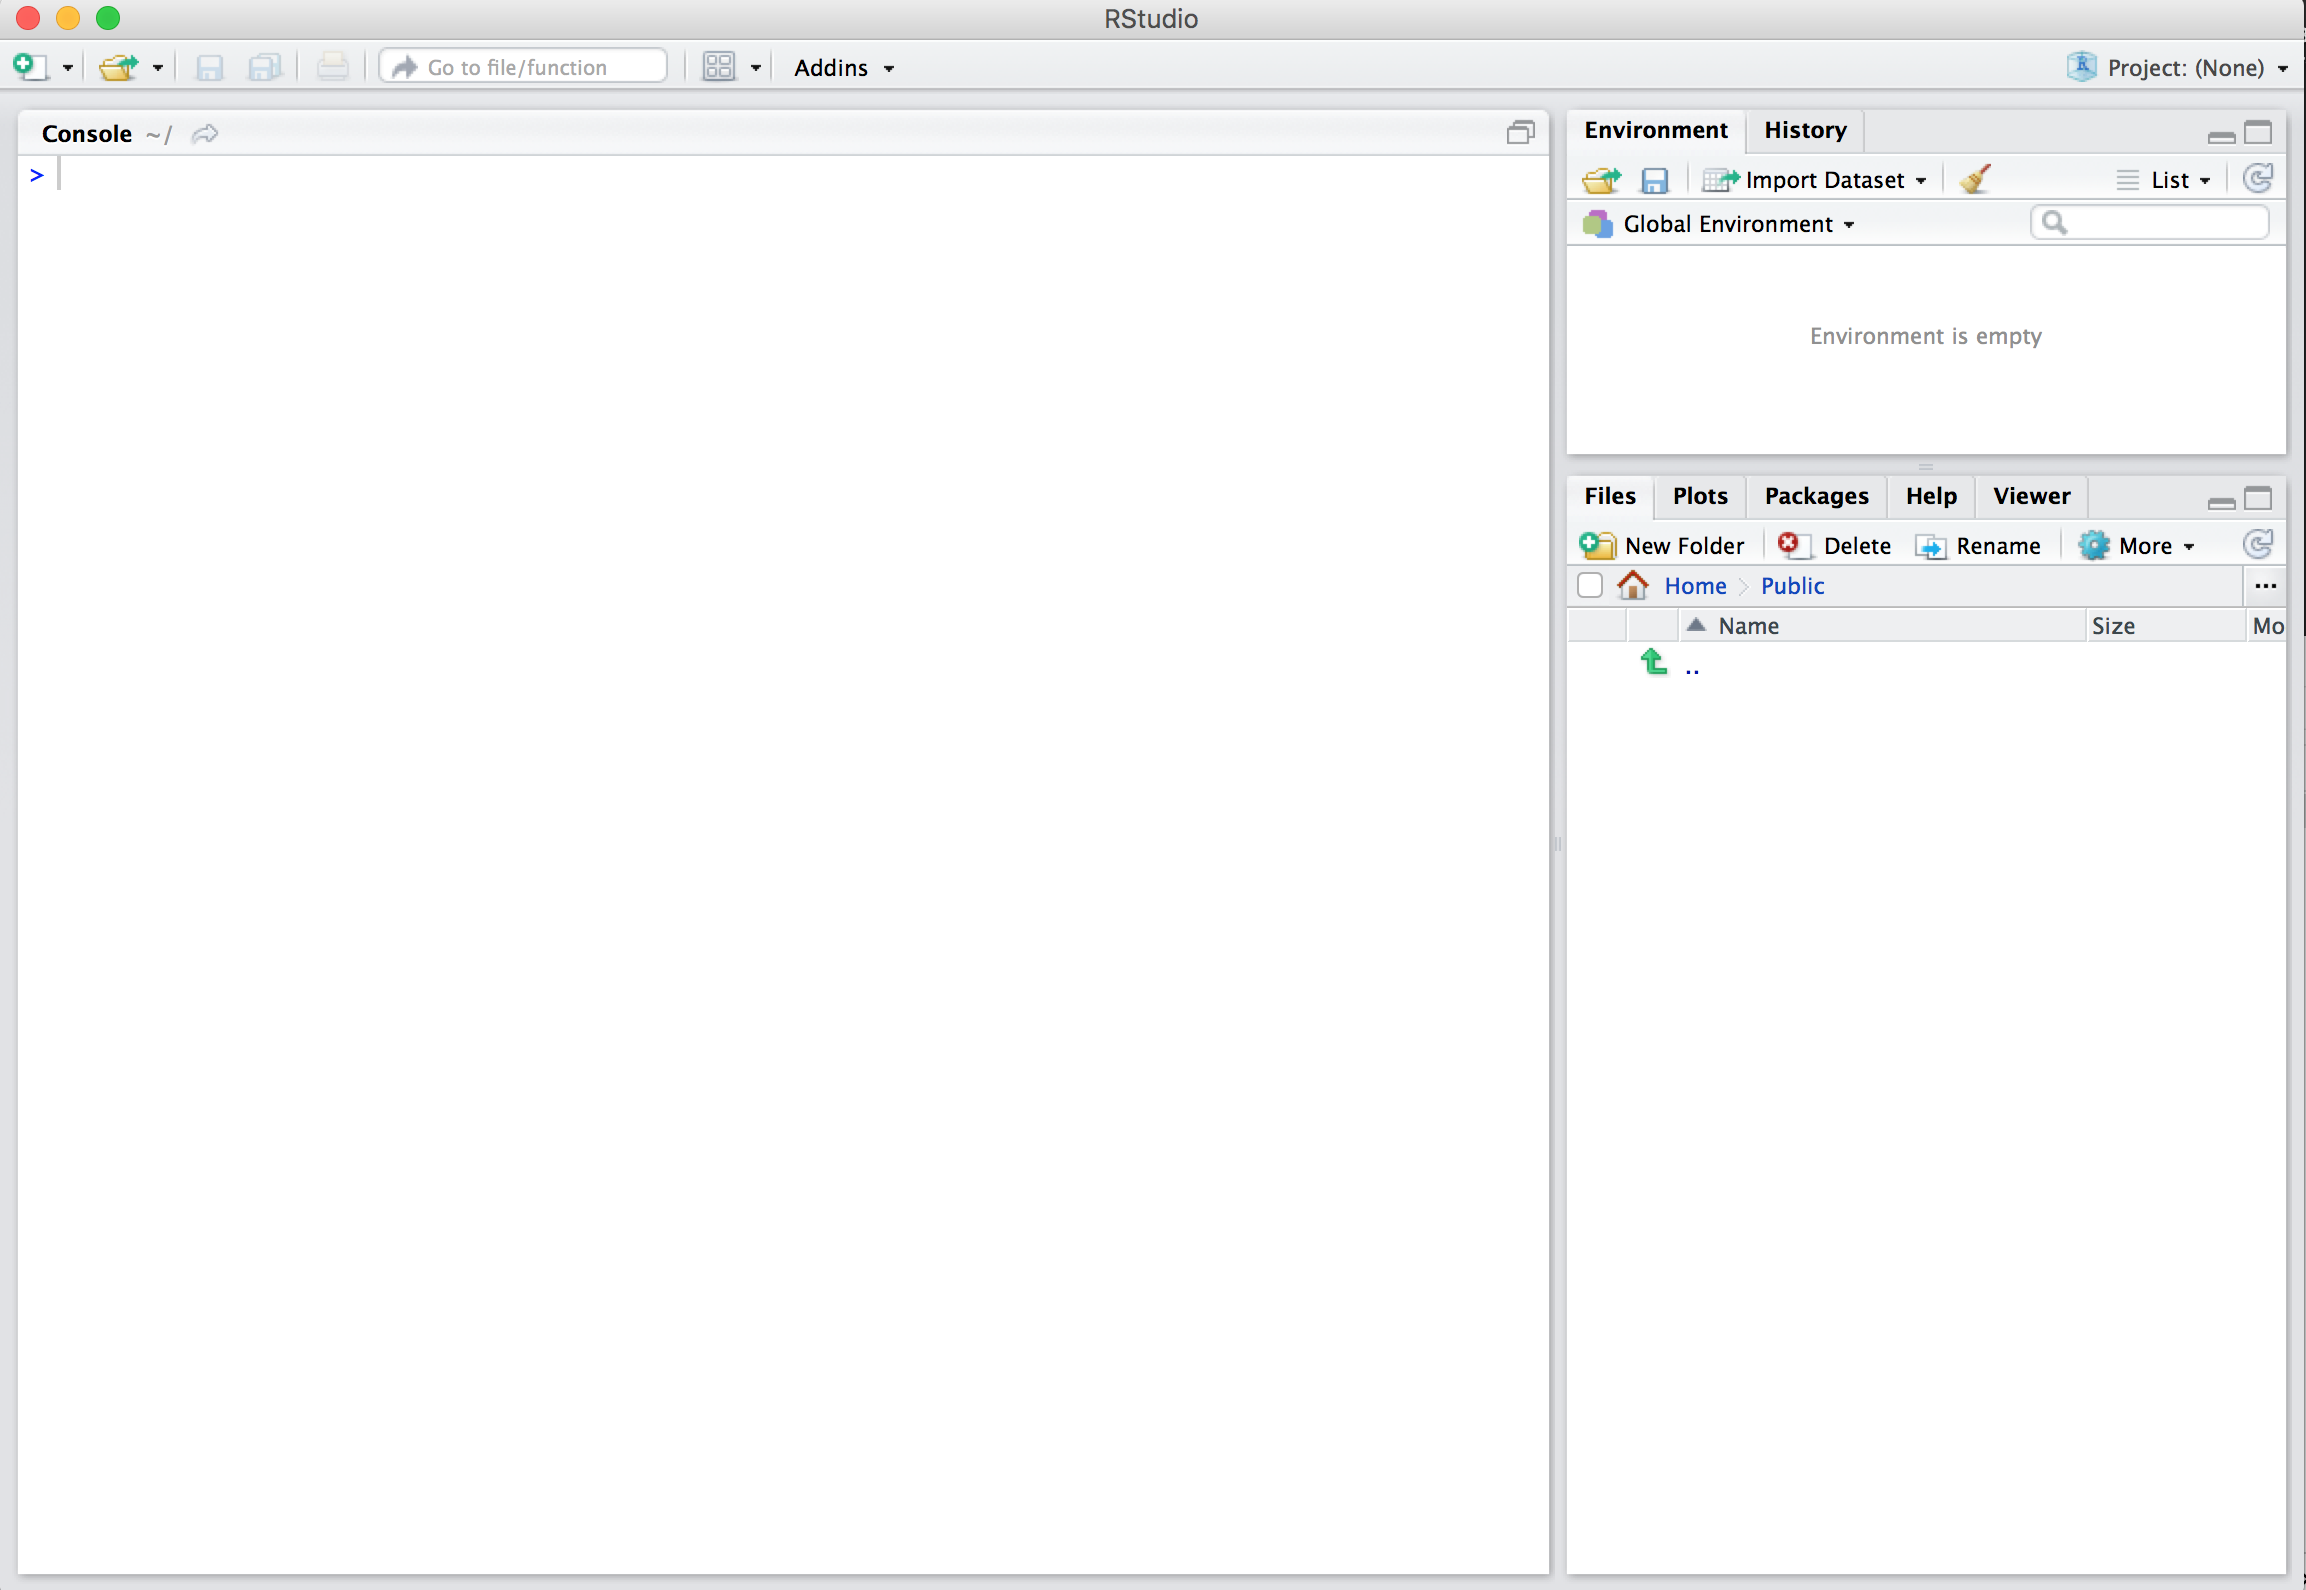
\includegraphics{images/rstudio.png}

Regardez
\href{https://campus.datacamp.com/courses/working-with-the-rstudio-ide-part-1/orientation?ex=5}{cette
vidéo DataCamp} pour découvrir les différents panneaux de l'application,
en particulier la Console dans laquelle nous executerons très bientôt du
code R

\begin{center}\rule{0.5\linewidth}{\linethickness}\end{center}

\hypertarget{code}{%
\subsection{Comment exécuter du code R ?}\label{code}}

Maintenant que vous avez configuré R et RStudio, vous vous demandez
probablement ``OK. Maintenant, comment utiliser R ?'' La première chose
à noter est que, contrairement à d'autres logiciels comme Excel, STATA
ou SAS qui fournissent des interfaces où tout se fait en cliquant avec
sa souris, R est un langage interprété, ce qui signifie que vous devez
entrer des commandes R écrites en code R. C'est-à-dire que vous devez
\textbf{programmer} en R (j'utilise les termes ``coder'' et
``programmer'' de manière interchangeable dans ce livre).

Il n'est pas nécessaire d'être un programmeur pour utiliser R. Néamnoins
il existe un ensemble de concepts de programmation de base que les
utilisateurs R doivent comprendre. Par conséquent, bien que ce livre ne
soit pas un livre sur la programmation, vous en apprendrez juste assez
sur ces concepts de programmation de base nécessaires pour explorer et
analyser efficacement des données.

\hypertarget{la-console}{%
\subsubsection{La console}\label{la-console}}

La façon la plus simle d'interagir avec RStudio (mais pas du tout la
meilleure !) consiste à taper directement des commandes que R pourra
comprendre dans la Console.

Cliquez dans la console (après le symbole \texttt{\textgreater{}}) et
tapez ceci, sans oublier de valider en tapant sur la touche
\texttt{Entrée} :

\begin{Shaded}
\begin{Highlighting}[]
\DecValTok{3} \OperatorTok{+}\StringTok{ }\DecValTok{8}
\end{Highlighting}
\end{Shaded}

\begin{verbatim}
[1] 11
\end{verbatim}

Félicitations, vous venez de taper votre première instruction R : vous
savez maintenant faire une addition !

\hypertarget{le-repertoire-de-travail}{%
\subsubsection{Le répertoire de
travail}\label{le-repertoire-de-travail}}

La première commande que vous devriez connaître quand vous travaillez
dans R ou RStudio est la suivante :

\begin{Shaded}
\begin{Highlighting}[]
\KeywordTok{getwd}\NormalTok{()}
\end{Highlighting}
\end{Shaded}

Si vous tapez cette commande dans la console, RStudio doit vous afficher
un emplacement sur votre ordinateur. Cet emplacement est appelé
``Répertoire de travail'', ou ``Working Directory'' en anglais
(\texttt{getwd()} est l'abbréviation de ``Get Working Directory'').

Ce répertoire de travail est important : c'est là que seront stockés les
tableaux et graphiques que vous déciderez de sauvegarder. C'est là aussi
que vous sauvegarderez vos scripts (voir plus bas) qui vous permettront
de garder la trace de votre travail et de le reprendre là où vous
l'aviez laissé la dernière fois. Enfin, lorsque vous souhaiterez
importer des tableaux de données contenus dans des fichiers externes
(par exemple, des fichiers Excel), c'est également dans ce répertoire
que R tentera de trouver vos données.

Avant d'aller plus loin je vous conseille donc vivement de :

\begin{enumerate}
\def\labelenumi{\arabic{enumi}.}
\tightlist
\item
  Créer un nouveau dossier intitulé ``Biometrie'' sur votre espace
  personnel (généralement, sur le disque ``W:'' des ordinateurs de
  l'Université)
\item
  Indiquez à RStudio que vous souhaitez travailler dans ce nouveau
  répertoire de travail. Pour cela vous avez 3 solutions au choix :

  \begin{enumerate}
  \def\labelenumii{\arabic{enumii}.}
  \tightlist
  \item
    Dans RStudio, cliquez dans le menu ``Session \textgreater{} Set
    Working Directory \textgreater{} Choose Directory\ldots{}'' puis
    naviguez jusqu'au dossier que vous venez de créer
  \item
    Dans le panneau ``Files'', naviguez jusqu'au dossier ``Biometrie''
    que vous venez de créer, puis cliquez sur le bouton ``More
    \textgreater{} Set As Working Directory''
  \item
    En ligne de commande, dans la console, utilisez la fonction
    \texttt{setwd()} pour spécifier le chemin de votre nouveau dossier,
    par exemple :
  \end{enumerate}
\end{enumerate}

\begin{Shaded}
\begin{Highlighting}[]
\CommentTok{# Attention à bien respecter les majuscules et à utiliser les guillemets.}
\KeywordTok{setwd}\NormalTok{(}\StringTok{"W:/Biometrie"}\NormalTok{)}
\end{Highlighting}
\end{Shaded}

Il ne vous reste plus qu'à vérifier que le changement a bien été pris en
compte en tapant à nouveau \texttt{getwd()} dans la console. Attention,
vous devez vous assurer d'être dans le bon répertoire de travil
\textbf{à chaque nouvelle session} !

\hypertarget{les-scripts}{%
\subsubsection{Les scripts}\label{les-scripts}}

Taper du code directement dans la console est probablement la pire façon
de travailler dans RStudio. Cela est parfois utile pour faire un rapide
calcul, ou pour vérifier qu'une commande fonctionne correctement. Mais
la plupart du temps, vous devriez taper vos commandes dans un script.

Un script est un fichier au format ``texte brut'' (cela signifie qu'il
n'y a pas de mise en forme et que ce fichier peut-être ouvert par
n'importe quel éditeur de texte, y compris les plus simples comme le
bloc notes de Windows), dans lequel vous pouvez taper :

\begin{enumerate}
\def\labelenumi{\arabic{enumi}.}
\tightlist
\item
  des instructions qui seront comprises par R comme si vous les tapiez
  directement dans la console
\item
  des lignes de commentaires, qui doivent obligatoirement commencer par
  le symbole \texttt{\#}.
\end{enumerate}

Les avantages de travailler dans un script sont nombreux :

\begin{enumerate}
\def\labelenumi{\arabic{enumi}.}
\tightlist
\item
  Vous pouvez sauvegarder votre script à tout moment (vous devriez
  prendre l'habitude de le sauvegarder très régulièrement). Vous gardez
  ainsi la trace de toutes les commandes que vous avez tapées.
\item
  Vous pouvez aisément partager votre script pour collaborer avec vos
  collègues de promo et enseignants.
\item
  Vous pouvez documenter votre démarche et les différentes étapes de vos
  analyses. Vous devez ajouter autant de commentaires que possible. Cela
  permettra à vos collaborateurs de comprendre ce que vous avez fait. Et
  cela vous permettra de comprendre ce que vous avez fait il y a 6 mois
  quand vous vous re-plongerez dans vos analyses dans quelques temps. Si
  votre démarche vous paraît cohérente maintenant, il n'est en effet pas
  garanti que vous rappellerez de chaque détail dans 6 mois ou 6 ans.
\item
  Un script bien structuré et clair permet de rendre vos analyses
  répétables. Si vous passer 15 heures à analyser un tableau de données
  précis, il vous suffira de quelques secondes pour analyser un nouveau
  jeu de données similaires : vous n'aurez que quelques lignes à
  modifier dans votre script original pour l'appliquer à de nouvelles
  données.
\end{enumerate}

Vous pouvez créer un script en cliquant dans le menu ``File
\textgreater{} New File \textgreater{} R Script''. Un nouveau panneau
s'ouvre dans l'application. Pensez à sauvegarder immédiatement votre
nouveau script. Il faut pour cela lui donner un nom. Vous noterez que
par défaut, RStudio propose d'enregistrer votre script dans votre
répertoire de travail.

À partir de maintenant, vous ne devriez plus taper de commande
directement dans la console. Tapez systématiquement vos commandes dans
un script et sauvegardez-le régulièrement.

Pour exécuter les commandes du script dans la console, il suffit de
placer le curseur sur la ligne contenant la commande et de presser les
touches \texttt{ctrl\ +\ enter} (ou \texttt{command\ +\ enter} sous
macOS). Si un message d'erreur s'affiche dans la console, c'est que
votre instruction était erronée. Modifiez la directement dans votre
script et pressez à nouveau les touches \texttt{ctrl\ +\ enter} (ou
\texttt{command\ +\ enter} sous macOS) pour tenter à nouveau votre
chance. Idéalement, votre script ne devrait contenir que des commandes
qui fonctionnent et des commentaires expliquant à quoi servent ces
commandes.

À la fin de chaque séance de TEA, vous devrez déposer sur l'ENT le
script que vous avez créé durant la séance. Ce script devra porter votre
nom de famille et se terminer par l'extension \texttt{.R}. Ainsi, si
Jean-Claude Van Damme faisait des statistiques, il devrait déposer sur
l'ENT un fichier intitulé \texttt{VanDamme.R} à la fin de chaque séance
de TEA.

Ci-dessous, un exemple de script

\begin{Shaded}
\begin{Highlighting}[]
\CommentTok{# Penser à installer le package ggplot2 si besoin install.packages('ggplot2')}

\CommentTok{# Chargement du package}
\KeywordTok{library}\NormalTok{(ggplot2)}

\CommentTok{# Mise en méoire des données de qualité de l'air à New-York de mai à septembre}
\CommentTok{# 1973}
\KeywordTok{data}\NormalTok{(airquality)}

\CommentTok{# Affichage des premières lignes du tableau de données}
\KeywordTok{head}\NormalTok{(airquality)}

\CommentTok{# Quelle est la structure de ce tableau ?}
\KeywordTok{str}\NormalTok{(airquality)}

\CommentTok{# Réalisation d'un graphique présentant la relation entre la concentration en}
\CommentTok{# ozone atmosphérique en ppb et la température en degrés Farenheit}
\KeywordTok{ggplot}\NormalTok{(}\DataTypeTok{data =}\NormalTok{ airquality, }\DataTypeTok{mapping =} \KeywordTok{aes}\NormalTok{(}\DataTypeTok{x =}\NormalTok{ Temp, }\DataTypeTok{y =}\NormalTok{ Ozone)) }\OperatorTok{+}\StringTok{ }\KeywordTok{geom_point}\NormalTok{() }\OperatorTok{+}\StringTok{ }\KeywordTok{geom_smooth}\NormalTok{(}\DataTypeTok{method =} \StringTok{"loess"}\NormalTok{)}

\CommentTok{# On constate une augmentation importante de la concentration d'ozone pour des}
\CommentTok{# températures supérieures à 75ºF}
\end{Highlighting}
\end{Shaded}

Même si vous ne comprenez pas encore les commandes qui figurent dans ce
script (ça viendra !), voici ce que vous devez en retenir :

\begin{enumerate}
\def\labelenumi{\arabic{enumi}.}
\tightlist
\item
  Le script contient plus de lignes de commentaires que de commandes R
\item
  Chaque étape de l'analyse est décrite en détail
\item
  On peut ajouter des commentaires afin de décrire les résultats
\item
  Seules les commandes pertinentes et qui fonctionnent ont été
  conservées dans ce script
\item
  Chaque ligne de commentaire commence par \texttt{\#}. Il est ainsi
  possible de conserver certaines commandes R dans le script, ``pour
  mémoire'', sans pour autant qu'elle ne soient exécutées. C'est le cas
  pour la ligne \texttt{\#\ install.packages("ggplot2")}.
\end{enumerate}

Si j'éxécute ce script dans la console de RStudio (en sélectionnant
toutes les lignes et en pressant les touches \texttt{ctrl+enter} ou
\texttt{command+enter} sous macOS), voilà ce qui est produit :

\begin{verbatim}
  Ozone Solar.R Wind Temp Month Day
1    41     190  7.4   67     5   1
2    36     118  8.0   72     5   2
3    12     149 12.6   74     5   3
4    18     313 11.5   62     5   4
5    NA      NA 14.3   56     5   5
6    28      NA 14.9   66     5   6
\end{verbatim}

\begin{verbatim}
'data.frame':   153 obs. of  6 variables:
 $ Ozone  : int  41 36 12 18 NA 28 23 19 8 NA ...
 $ Solar.R: int  190 118 149 313 NA NA 299 99 19 194 ...
 $ Wind   : num  7.4 8 12.6 11.5 14.3 14.9 8.6 13.8 20.1 8.6 ...
 $ Temp   : int  67 72 74 62 56 66 65 59 61 69 ...
 $ Month  : int  5 5 5 5 5 5 5 5 5 5 ...
 $ Day    : int  1 2 3 4 5 6 7 8 9 10 ...
\end{verbatim}

\begin{center}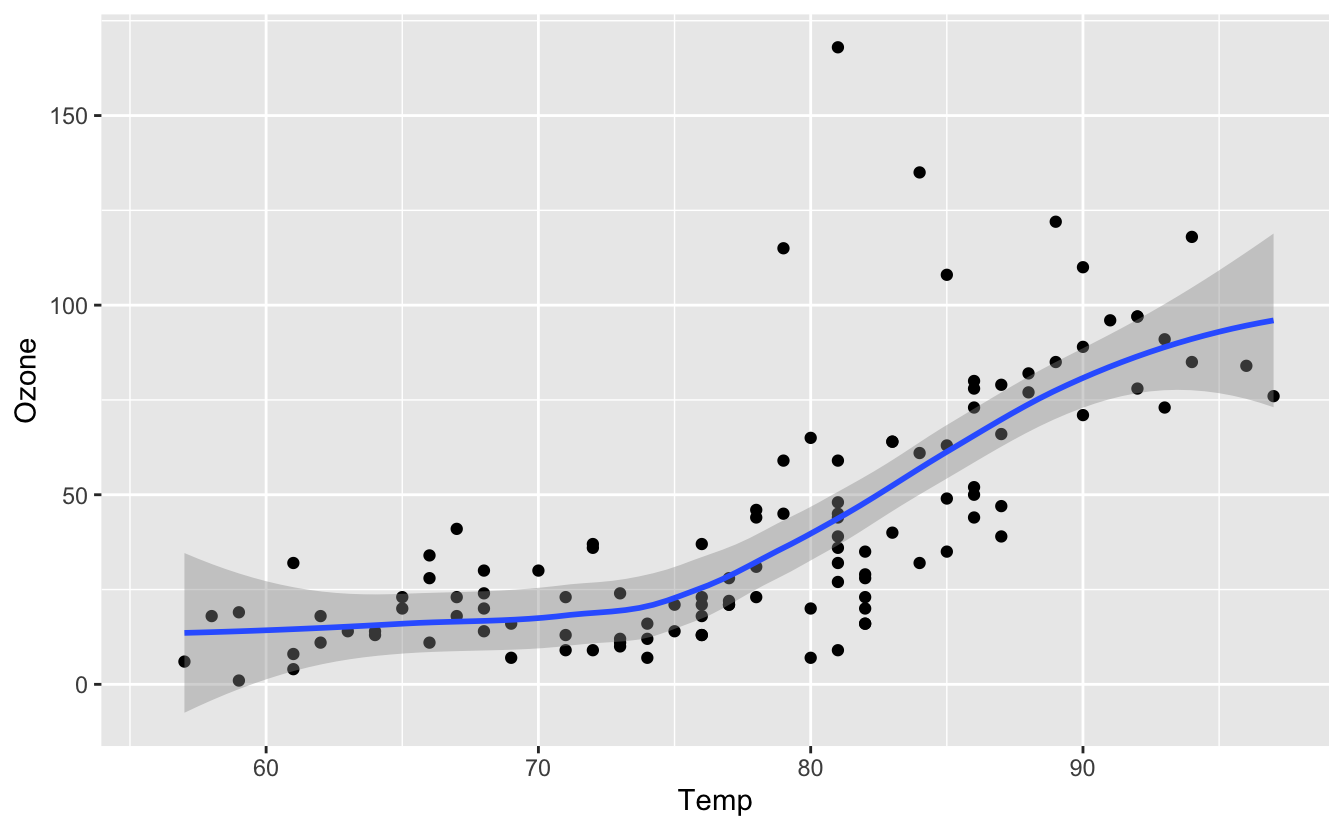
\includegraphics[width=0.9\linewidth]{figure/unnamed-chunk-5-1} \end{center}

\hypertarget{concepts-de-base-en-programmation-et-terminologie}{%
\subsubsection{Concepts de base en programmation et
terminologie}\label{concepts-de-base-en-programmation-et-terminologie}}

Pour vous présenter les concepts de base et la terminologie de la
programmation dont nous aurons besoin dans R, vous allez suivre les
tutoriels en ligne suivants, sur le site de DataCamp. Pour chacun des
tutoriels, j'indique une liste des concepts de programmation couverts.
Notez que dans ce livre, nous utiliserons une police différente pour
distinguer le texte normal et les \texttt{commandes-informatiques}.

Il est important de noter que, bien que ces tutoriels sont d'excellentes
introductions, une seule lecture est insuffisante pour un apprentissage
en profondeur et une rétention à long terme. Les outils ultimes pour
l'apprentissage et la rétention à long terme sont ``l'apprentissage par
la pratique'' et ``la répétition''. Outre les exercices demandés dans
DataCamp, que vous devez effectuer directement dans votre navigateur, je
vous encourage donc à multiplier les essais, directement dans la console
de RStudio, ou, de préférence, dans un script que vous annoterez, pour
vous assurer que vous avez bien compris chaque partie.

\hypertarget{objects}{%
\paragraph{Objets, types, vecteurs, facteurs et tableaux de
données}\label{objects}}

Dans
\href{https://www.datacamp.com/community/open-courses/introduction-a-r}{le
cours d'introduction à R} sur DataCamp, suivez les chapitres suivants.
Au fur et à mesure de votre travail, notez les termes importants et ce à
quoi ils font référence.

\begin{itemize}
\tightlist
\item
  \href{https://campus.datacamp.com/courses/introduction-a-r/chapitre-1-introduction?ex=1}{Chapitre
  1 : introduction}

  \begin{itemize}
  \tightlist
  \item
    La console : l'endroit où vous tapez des commandes
  \item
    Les objets : où les valeurs sont stockées, comment assigner des
    valeurs à des objets
  \item
    Les types de données : entiers, doubles/numériques, charactères et
    logiques
  \end{itemize}
\item
  \href{https://campus.datacamp.com/courses/introduction-a-r/chapitre-2-les-vecteurs?ex=1}{Chapitre
  2 : vecteurs}

  \begin{itemize}
  \tightlist
  \item
    Les vecteurs : des collections de valeurs du même type.
  \end{itemize}
\item
  \href{https://campus.datacamp.com/courses/introduction-a-r/chapitre-4-facteurs?ex=1}{Chapitre
  4 : les facteurs}

  \begin{itemize}
  \tightlist
  \item
    Des données catégorielles (et non pas \emph{numériques}) représentés
    dans R sous forme de \texttt{factor}s.
  \end{itemize}
\item
  \href{https://campus.datacamp.com/courses/introduction-a-r/chapitre-5-les-jeux-de-donnees?ex=1}{Chapitre
  5 : les jeux de données ou \texttt{data.frame}}

  \begin{itemize}
  \tightlist
  \item
    Les \texttt{data.frame}s sont similaires aux feuilles de calcul
    rectangulaires que l'on peut produire dans un tableur. Dans R, ce
    sont des objets rectangulaires (des tableaux !) contenant des jeux
    de jeux de données : les lignes correspondent aux observations et
    les colonnes aux variables décrivant les observations. La plupart du
    temps, c'es le format de données que nous utiliserons. Plus de
    détails dans la partie \ref{dataset}.
  \end{itemize}
\end{itemize}

Avant de passer à la suite, il nous reste 2 grandes notions à découvrir
dans le domaine du code et de la syntaxe afin de pouvoir travailler
efficacement dans R : les opérateurs de comparaison d'une part, et les
fonctions d'autre part.

\hypertarget{comparaison}{%
\paragraph{Opérateurs de comparaison}\label{comparaison}}

Comme leur nom l'indique, ils permettent de comparer des valeurs ou des
objets. Les principaux opérateurs de comparaison sont :

\begin{itemize}
\tightlist
\item
  \texttt{==} : égale à
\item
  \texttt{!=} : différent de
\item
  \texttt{\textgreater{}} : supérieur à
\item
  \texttt{\textless{}} : inférieur à
\item
  \texttt{\textgreater{}=} : supérieur ou égal à
\item
  \texttt{\textless{}=} : inférieur ou égal à
\end{itemize}

Ainsi, on peut tester si 3 est égal à 5 :

\begin{Shaded}
\begin{Highlighting}[]
\DecValTok{3} \OperatorTok{==}\StringTok{ }\DecValTok{5}
\end{Highlighting}
\end{Shaded}

\begin{verbatim}
[1] FALSE
\end{verbatim}

La réponse est bien entendu \texttt{FALSE}. Est-ce que 3 est inférieur à
5 ?

\begin{Shaded}
\begin{Highlighting}[]
\DecValTok{3} \OperatorTok{<}\StringTok{ }\DecValTok{5}
\end{Highlighting}
\end{Shaded}

\begin{verbatim}
[1] TRUE
\end{verbatim}

La réponse est maintenant \texttt{TRUE}. Lorsque l'on utilise un
opérateur de comparaison, la réponse est toujours soit vrai
(\texttt{TRUE}), soit faux (\texttt{FALSE}).

Il est aussi possible de comparer des chaînes de charactères :

\begin{Shaded}
\begin{Highlighting}[]
\StringTok{"Bonjour"} \OperatorTok{==}\StringTok{ "Au revoir"}
\end{Highlighting}
\end{Shaded}

\begin{verbatim}
[1] FALSE
\end{verbatim}

\begin{Shaded}
\begin{Highlighting}[]
\StringTok{"Bonjour"} \OperatorTok{>=}\StringTok{ "Au revoir"}
\end{Highlighting}
\end{Shaded}

\begin{verbatim}
[1] TRUE
\end{verbatim}

Manifestement, ``Bonjour'' est supérieur ou égal à ``Au revoir''. En
fait, R utilise l'ordre alphabétique pour comparer les chaînes de
caractères. Puisque dans l'alphabet, le ``B'' de ``Bonjour'' arrive
après le ``A'' de ``Au revoir'', pour R, ``Bonjour'' est bien supérieur
à ``Au revoir''.

Il est également possible d'utiliser ces opérateurs pour comparer un
chiffre et un vecteur :

\begin{Shaded}
\begin{Highlighting}[]
\NormalTok{tailles_pop1 <-}\StringTok{ }\KeywordTok{c}\NormalTok{(}\DecValTok{112}\NormalTok{, }\DecValTok{28}\NormalTok{, }\DecValTok{86}\NormalTok{, }\DecValTok{14}\NormalTok{, }\DecValTok{154}\NormalTok{, }\DecValTok{73}\NormalTok{, }\DecValTok{63}\NormalTok{, }\DecValTok{48}\NormalTok{)}
\NormalTok{tailles_pop1 }\OperatorTok{>}\StringTok{ }\DecValTok{80}
\end{Highlighting}
\end{Shaded}

\begin{verbatim}
[1]  TRUE FALSE  TRUE FALSE  TRUE FALSE FALSE FALSE
\end{verbatim}

Ici, l'opérateur nous permet d'identifier quels éléments du vecteur
\texttt{taille\_pop1} sont supérieurs à 80. Il s'agit des éléments
placés en première, troisième et cinquième position.

Il est aussi possible de comparer 2 vecteurs qui contiennent le même
nombre d'éléments :

\begin{Shaded}
\begin{Highlighting}[]
\NormalTok{tailles_pop2 <-}\StringTok{ }\KeywordTok{c}\NormalTok{(}\DecValTok{114}\NormalTok{, }\DecValTok{27}\NormalTok{, }\DecValTok{38}\NormalTok{, }\DecValTok{91}\NormalTok{, }\DecValTok{54}\NormalTok{, }\DecValTok{83}\NormalTok{, }\DecValTok{33}\NormalTok{, }\DecValTok{68}\NormalTok{)}
\NormalTok{tailles_pop1 }\OperatorTok{>}\StringTok{ }\NormalTok{tailles_pop2}
\end{Highlighting}
\end{Shaded}

\begin{verbatim}
[1] FALSE  TRUE  TRUE FALSE  TRUE FALSE  TRUE FALSE
\end{verbatim}

Les comparaisons sont ici faites élément par élément. Ainsi, les
observations 2, 3, 5 et 7 du vecteur \texttt{tailles\_pop1} sont
supérieures aux observations 2, 3, 5 et 7 du vecteur
\texttt{tailles\_pop2} respectivement.

Ces vecteurs de vrais/faux sont très utiles car ils peuvent permettre de
compter le nombre d'éléments répondant à une certains condition :

\begin{Shaded}
\begin{Highlighting}[]
\KeywordTok{sum}\NormalTok{(tailles_pop1 }\OperatorTok{>}\StringTok{ }\NormalTok{tailles_pop2)}
\end{Highlighting}
\end{Shaded}

\begin{verbatim}
[1] 4
\end{verbatim}

Lorsque l'on effectue une opération arithmétique (comme le calcul d'une
somme ou d'une moyenne) sur un vecteur de vrais/faux, les \texttt{TRUE}
sont remplacés par \texttt{1} et les \texttt{FALSE} par \texttt{0}. La
somme nous indique donc le nombre de vrais dans un vecteur de
vrais/faux, et la moyenne nous indique la proportion de vrais :

\begin{Shaded}
\begin{Highlighting}[]
\KeywordTok{mean}\NormalTok{(tailles_pop1 }\OperatorTok{>}\StringTok{ }\NormalTok{tailles_pop2)}
\end{Highlighting}
\end{Shaded}

\begin{verbatim}
[1] 0.5
\end{verbatim}

\textbf{Note} : Attention, si les vecteurs comparés n'ont pas la même
taille, un message d'avertissement est affiché :

\begin{Shaded}
\begin{Highlighting}[]
\NormalTok{tailles_pop3 <-}\StringTok{ }\KeywordTok{c}\NormalTok{(}\DecValTok{43}\NormalTok{, }\DecValTok{56}\NormalTok{, }\DecValTok{92}\NormalTok{)}
\NormalTok{tailles_pop1}
\end{Highlighting}
\end{Shaded}

\begin{verbatim}
[1] 112  28  86  14 154  73  63  48
\end{verbatim}

\begin{Shaded}
\begin{Highlighting}[]
\NormalTok{tailles_pop3}
\end{Highlighting}
\end{Shaded}

\begin{verbatim}
[1] 43 56 92
\end{verbatim}

\begin{Shaded}
\begin{Highlighting}[]
\NormalTok{tailles_pop3 }\OperatorTok{>}\StringTok{ }\NormalTok{tailles_pop1}
\end{Highlighting}
\end{Shaded}

\begin{verbatim}
Warning in tailles_pop3 > tailles_pop1: la taille d'un objet plus long n'est pas
multiple de la taille d'un objet plus court
\end{verbatim}

\begin{verbatim}
[1] FALSE  TRUE  TRUE  TRUE FALSE  TRUE FALSE  TRUE
\end{verbatim}

Dans un cas comme celui là, R va \emph{recycler} l'objet le plus court,
ici \texttt{tailles\_pop3} pour qu'une comparaison puisse être faite
avec chaque élément de l'objet le plus long (ici,
\texttt{tailles\_pop1}). Ainsi, 43 est comparé à 112, 56 est comparé à
28 et 92 est comparé à 86. Puisque \texttt{tailles\_pop3} ne contient
plus d'éléments, ils sont recyclés, dans le même ordre : 43 est comparé
à 14, 56 est comparé à 154, et ainsi de suite jusqu'à ce que tous les
éléments de \texttt{tailles\_pop1} aient été passés en revue.

Ce type de recyclage est très risqué car il est difficile de savoir ce
qui a été comparé avec quoi. En travaillant avec des tableaux plutôt
qu'avec des vecteurs, le problème est généralement évité puisque toutes
les colonnes d'un \texttt{data.frame} contiennent le même nombre
d'éléments.

Dernière chose concernant les opérateurs de comparaison : la question
des données manquantes. Dans R les données manquantes sont symbolisées
par cette notation : \texttt{NA}, abréviation de ``Not Available''. Le
symbole \texttt{NaN} est parfois aussi observé lorsque des opérations
ont conduit à des indéterminations. Mais c'est plus rare et la plupart
du temps, les \texttt{NaN}s peuvent être traités comme les \texttt{NA}s.
L'un des problèmes des données manquantes, est qu'il est nécessaire de
prendre des précautions pour réaliser des comparaison les impliquants :

\begin{Shaded}
\begin{Highlighting}[]
\DecValTok{3} \OperatorTok{==}\StringTok{ }\OtherTok{NA}
\end{Highlighting}
\end{Shaded}

\begin{verbatim}
[1] NA
\end{verbatim}

On s'attend logiquement à ce que 3 ne soit pas considéré comme égal à
\texttt{NA}, et donc, on s'attend à obtenir \texttt{FALSE}. Pourtant, le
résultat est \texttt{NA}. La comparaison d'un élément quelconque à une
donnée manquante fournit toujours une donnée manquante : la comparaison
ne peut pas se faire, R n'a donc rien à retourner. C'est également le
cas aussi lorsque l'on compare deux valeurs manquantes :

\begin{Shaded}
\begin{Highlighting}[]
\OtherTok{NA} \OperatorTok{==}\StringTok{ }\OtherTok{NA}
\end{Highlighting}
\end{Shaded}

\begin{verbatim}
[1] NA
\end{verbatim}

C'est pourtant assez logique. Imaginons que j'ignore l'âge de Pierre et
l'âge de Marie. Il n'y a aucune raison pour que leur âge soit le même,
mais il est tout à fait possible qu'il le soit. C'est impossible à
déterminer :

\begin{Shaded}
\begin{Highlighting}[]
\NormalTok{age_Pierre <-}\StringTok{ }\OtherTok{NA}
\NormalTok{age_Marie <-}\StringTok{ }\OtherTok{NA}
\NormalTok{age_Pierre }\OperatorTok{==}\StringTok{ }\NormalTok{age_Marie}
\end{Highlighting}
\end{Shaded}

\begin{verbatim}
[1] NA
\end{verbatim}

Mais alors comment faire pour savoir si une valeur est manquante
puisqu'on ne peut pas utiliser les opérateurs de comparaison ? On
utilise la fonction \texttt{is.na()} :

\begin{Shaded}
\begin{Highlighting}[]
\KeywordTok{is.na}\NormalTok{(age_Pierre)}
\end{Highlighting}
\end{Shaded}

\begin{verbatim}
[1] TRUE
\end{verbatim}

\begin{Shaded}
\begin{Highlighting}[]
\KeywordTok{is.na}\NormalTok{(tailles_pop3)}
\end{Highlighting}
\end{Shaded}

\begin{verbatim}
[1] FALSE FALSE FALSE
\end{verbatim}

D'une façon générale, le point d'exclamation permet de signifier à R que
nous souhaitons obtenir le contraire d'une expression :

\begin{Shaded}
\begin{Highlighting}[]
\OperatorTok{!}\KeywordTok{is.na}\NormalTok{(age_Pierre)}
\end{Highlighting}
\end{Shaded}

\begin{verbatim}
[1] FALSE
\end{verbatim}

\begin{Shaded}
\begin{Highlighting}[]
\OperatorTok{!}\KeywordTok{is.na}\NormalTok{(tailles_pop3)}
\end{Highlighting}
\end{Shaded}

\begin{verbatim}
[1] TRUE TRUE TRUE
\end{verbatim}

Cette fonction nous sera très utile plus tard pour éliminer toutes les
lignes d'un tableau contenant des valeurs manquantes.

\hypertarget{functions}{%
\paragraph{L'utilisation des fonctions}\label{functions}}

Dans R, les fonctions sont des objets particuliers qui permettent
d'effectuer des tâches très variées. Du calcul d'une moyenne à la
création d'un graphique, en passant par la réalisation d'analyses
statistiques complexes ou simplement l'affichage du chemin du répertoire
de travail, tout, dans R, repose sur l'utilisation de fonctions. Vous en
avez déjà vu un certain nombre :

\begin{longtable}[]{@{}rl@{}}
\toprule
Fonction & Pour quoi faire ?\tabularnewline
\midrule
\endhead
\texttt{c()} & Créer des vecteurs\tabularnewline
\texttt{class()} & Afficher ou modifier la classe d'un
objet\tabularnewline
\texttt{factor()} & Créer des facteurs\tabularnewline
\texttt{getwd()} & Afficher le chemin du répertoire de
travail\tabularnewline
\texttt{head()} & Afficher les premiers éléments d'un
objet\tabularnewline
\texttt{is.na()} & Tester si un objet contient des valeurs
manquantes\tabularnewline
\texttt{mean()} & Calculer une moyenne\tabularnewline
\texttt{names()} & Afficher ou modifier le nom des éléments d'un
vecteur\tabularnewline
\texttt{order()} & Ordonner les éléments d'un objet\tabularnewline
\texttt{setwd()} & Modifier le chemin du répertoire de
travail\tabularnewline
\texttt{subset()} & Extraire une partie des éléments d'un
objet\tabularnewline
\texttt{sum()} & Calculer une somme\tabularnewline
\texttt{tail()} & Afficher les derniers éléments d'un
objet\tabularnewline
\bottomrule
\end{longtable}

Cette liste va très rapidement s'allonger au fil des séances. Je vous
conseille donc vivement de tenir à jour une liste des fonctions
décrites, avec une explication de leur fonctionnement et éventuellement
un exemple de syntaxe.

Certaines fonction ont besoin d'arguments (par exemple, la fonction
\texttt{factor()}), d'autres peuvent s'en passer (par exemple, la
fonction \texttt{getwd()}). Pour apprendre comment utiliser une fonction
particulière, pour découvrir quels sont ses arguments possibles, quelle
est leur rôle et leur intérêt, la meilleure solution est de consulter
l'aide de cette fonction. Il suffit pour cela de taper un \texttt{?}
suivi du nom de la fonction :

\begin{Shaded}
\begin{Highlighting}[]
\NormalTok{?}\KeywordTok{factor}\NormalTok{()}
\end{Highlighting}
\end{Shaded}

Toutes les fonctions et jeux de données disponibles dans R disposent
d'un fichier d'aide similaire. Cela peut faire un peu peur au premier
abord (tout est en anglais !), mais ces fichiers d'aide ont l'avantage
d'être très complets, de fournir des exemples d'utilisation, et ils sont
tous construits sur le même modèle. Vous avez donc tout intérêt à vous
familiariser avec eux. vous devriez d'ailleurs prendre l'habitude de
consulter l'aide de chaque fonction qui vous pose un problème. Par
exemple, le logarithme (en base 10) de 100 devrait faire 2, car 100 est
égal à 10\^{}2. Pourtant :

\begin{Shaded}
\begin{Highlighting}[]
\KeywordTok{log}\NormalTok{(}\DecValTok{100}\NormalTok{)}
\end{Highlighting}
\end{Shaded}

\begin{verbatim}
[1] 4.60517
\end{verbatim}

Que se passe-t'il ? Pour le savoir, il faut consulter l'aide de la
fonction log :

\begin{Shaded}
\begin{Highlighting}[]
\NormalTok{?}\KeywordTok{log}\NormalTok{()}
\end{Highlighting}
\end{Shaded}

Ce fichier d'aide nous apprend que par défaut, la syntaxe de la fonction
\texttt{log()} est la suivante :

\begin{Shaded}
\begin{Highlighting}[]
\KeywordTok{log}\NormalTok{(x, }\DataTypeTok{base =} \KeywordTok{exp}\NormalTok{(}\DecValTok{1}\NormalTok{))}
\end{Highlighting}
\end{Shaded}

Par défaut, la base du logarithme est fixée à \texttt{exp(1)}. Nous
avons donc calculé un logarithme népérien (en base \emph{e}). Cette
fonction prend donc 2 arguments : 1. \texttt{x} ne possède pas de valeur
par défaut : il nous faut obligatoirement fournir quelque chose (la
rubrique ``Argument'' du fichier d'aide nous indique que \texttt{x} doit
être un vecteur numérique ou complexe) afin que la fonction puisse
calculer un logarithme 2. \texttt{base} possède un argument par défaut.
Si nous ne spécifions pas nous même la valeur de \texttt{base}, elle
sera fixée à sa valeur par défaut, c'est à dire \texttt{exp(1)}.

Pour calculer le logarithme en base 10 de 100, il faut donc taper, au
choix, l'une de ces 3 expressions :

\begin{Shaded}
\begin{Highlighting}[]
\KeywordTok{log}\NormalTok{(}\DataTypeTok{x =} \DecValTok{100}\NormalTok{, }\DataTypeTok{base =} \DecValTok{10}\NormalTok{)}
\end{Highlighting}
\end{Shaded}

\begin{verbatim}
[1] 2
\end{verbatim}

\begin{Shaded}
\begin{Highlighting}[]
\KeywordTok{log}\NormalTok{(}\DecValTok{100}\NormalTok{, }\DataTypeTok{base =} \DecValTok{10}\NormalTok{)}
\end{Highlighting}
\end{Shaded}

\begin{verbatim}
[1] 2
\end{verbatim}

\begin{Shaded}
\begin{Highlighting}[]
\KeywordTok{log}\NormalTok{(}\DecValTok{100}\NormalTok{, }\DecValTok{10}\NormalTok{)}
\end{Highlighting}
\end{Shaded}

\begin{verbatim}
[1] 2
\end{verbatim}

Le nom des arguments d'une fonction peut être omis tant que ces
arguments sont indiqués dans l'ordre attendu par la fonction (cet ordre
est celui qui est précisé à la rubrique ``Usage'' du fichier d'aide de
la fonction). Il est possible de modifier l'ordre des arguments d'une
fonction, mais il faut alors être parfaitement explicite et utiliser les
noms des arguments tels que définis dans le fichier d'aide.

Ainsi, pour calculer le logarithme en base 10 de 100, on ne peut pas
taper :

\begin{Shaded}
\begin{Highlighting}[]
\KeywordTok{log}\NormalTok{(}\DecValTok{10}\NormalTok{, }\DecValTok{100}\NormalTok{)}
\end{Highlighting}
\end{Shaded}

\begin{verbatim}
[1] 0.5
\end{verbatim}

car cela revient à calculer le logarithme en base 100 de 10. On peut en
revanche taper :

\begin{Shaded}
\begin{Highlighting}[]
\KeywordTok{log}\NormalTok{(}\DataTypeTok{base =} \DecValTok{10}\NormalTok{, }\DataTypeTok{x =} \DecValTok{100}\NormalTok{)}
\end{Highlighting}
\end{Shaded}

\begin{verbatim}
[1] 2
\end{verbatim}

\begin{center}\rule{0.5\linewidth}{\linethickness}\end{center}

\hypertarget{packages}{%
\subsection{Les packages additionels}\label{packages}}

Une source de confusion importante pour les nouveaux utilisateurs de R
est la notion de package. Les packages étendent les fonctionnalités de R
en fournissant des fonctions, des données et de la documentation
supplémentaires et peuvent être téléchargés gratuitement sur Internet.
Ils sont écrits par une communauté mondiale d'utilisateurs R. Par
exemple, parmi plus de 13000 packages disponibles à l'heure actuelle,
nous utiliseront fréquemment :

\begin{itemize}
\tightlist
\item
  Le package \texttt{ggplot2} pour la visualisation des données dans le
  chapitre \ref{viz}
\item
  Le package \texttt{dplyr} pour les manipuler des tableaux données dans
  le chapitre \ref{wrangling}
\end{itemize}

Il y a deux choses importantes à retenir à propos des packages R :

\begin{enumerate}
\def\labelenumi{\arabic{enumi}.}
\tightlist
\item
  \emph{Installation} : la plupart des packages ne sont pas installés
  par défaut lorsque vous installez R et RStudio. Vous devez installer
  un package avant de pouvoir l'utiliser. Une fois que vous l'avez
  installé, vous n'avez probablement pas besoin de l'installer à
  nouveau, sauf si vous souhaitez le mettre à jour vers une version plus
  récente du package.
\item
  \emph{Chargement} : les packages ne sont pas chargés automatiquement
  lorsque vous ouvrez RStudio. Vous devez les charger chaque fois que
  vous ouvrez RStudio en utilisant la commande \texttt{library\ ()}.
\end{enumerate}

Une bonne analogie pour les packages R : ils sont comme les apps que
vous téléchargez sur un téléphone portable :

\begin{longtable}[]{@{}cc@{}}
\toprule
R : Un nouveau téléphone & Packages: Apps qu'on peut
telécharger\tabularnewline
\midrule
\endhead
&\tabularnewline
\bottomrule
\end{longtable}

\begin{enumerate}
\def\labelenumi{\arabic{enumi}.}
\tightlist
\item
  R est comme un nouveau téléphone mobile. Il est capable de faire
  certaines choses lorsque vous l'utilisez pour la première fois, mais
  il ne sait pas tout faire.
\item
  Les packages R sont comme les apps que vous pouvez télécharger dans
  l'App Store et Google Play.
\item
  Pour utiliser un package, comme pour utiliser Instagram, vous devez :
  ~~~~ 1. Le télécharger et l'installer. Vous ne le faites qu'une fois.
  ~~~~ 1. Le charger (en d'autres termes, l'ouvrir) en utilisant la
  commande \texttt{library\ ()}.
\end{enumerate}

Donc, tout comme vous ne pouvez commencer à partager des photos avec vos
amis sur Instagram que si vous installez d'abord l'application et que
vous l'ouvrez, vous ne pouvez accéder aux données et fonctions d'un
package R que si vous installez d'abord le package et le chargez avec la
fonction \texttt{library()}. Passons en revue ces 2 étapes.

\hypertarget{installation-dun-package}{%
\subsubsection{Installation d'un
package}\label{installation-dun-package}}

Il y a deux façons d'installer un package. Par example, pour installer
le package \texttt{ggplot2} :

\begin{enumerate}
\def\labelenumi{\arabic{enumi}.}
\tightlist
\item
  \textbf{Le plus simple} : Dans le panneau ``File'' de Rstudio :

  \begin{enumerate}
  \def\labelenumii{\alph{enumii})}
  \tightlist
  \item
    Cliquez sur l'onglet ``Packages''
  \item
    Cliquez sur ``Install''
  \item
    Tapez le nom du package dans le champ ``Packages (separate multiple
    with space or comma):'' Pour notre exemple, tapez \texttt{ggplot2}
  \item
    Cliquez ``Install''
  \end{enumerate}
\item
  \textbf{Métode alternative} : Dans la console, tapez
  \texttt{install.packages("ggplot2")} (vous devez inclure les
  guillemets).
\end{enumerate}

En procédant de l'une ou l'autre façon, installez également les packages
suivants : \texttt{tidyverse} et \texttt{nycflights13}.

\textbf{Note} : un package doit être installé une fois seulement, sauf
si une version plus récente est disponible et que vous souhaitez mettre
à jour ce package.

\hypertarget{charger-un-package-en-memoire}{%
\subsubsection{Charger un package en
mémoire}\label{charger-un-package-en-memoire}}

Après avoir installé un package, vous pouvez le charger en utilisant la
fonction \texttt{library()}. Par exemple, pour charger \texttt{ggplot2}
et \texttt{dplyr} tapez ceci dans la console :

\begin{Shaded}
\begin{Highlighting}[]
\KeywordTok{library}\NormalTok{(ggplot2)}
\KeywordTok{library}\NormalTok{(dplyr)}
\end{Highlighting}
\end{Shaded}

\textbf{Note} : Vous devez charger à nouveau chaque package que vous
souhaitez utiliser à chaque fois que vous ouvrez une nouvelle session de
travail dans RStudio. Ça peut être un peu pénible et c'est une source
d'erreur fréquente pour les débutants. Quand vous vouyez un message
d'erreur commençant par :

\begin{verbatim}
Error: could not find function...
\end{verbatim}

rappelez-vous que c'est probablement parce que vous tentez d'utiliser
une fonction qui fait partie d'un package que vous n'avez pas chargé.
Pour corriger l'erreur, il suffit donc de charger le package approprié
avec la commande \texttt{library()}.

\begin{center}\rule{0.5\linewidth}{\linethickness}\end{center}

\hypertarget{exercices}{%
\subsection{Exercices}\label{exercices}}

Créez un nouveau script que vous nommerez \texttt{VotreNomDeFamille.R}.
Vous prendrez soin d'ajouter autant de commentaires que nécessaire dans
votre script afin de le structurer correctement.

\begin{enumerate}
\def\labelenumi{\arabic{enumi}.}
\tightlist
\item
  Téléchargez (si besoin) et chagez le package \texttt{ggplot2}
\item
  Chargez le jeu de données \texttt{diamonds} grâce à la commande
  \texttt{data(diamonds)}
\item
  Déterminer le nombre de lignes et de colonnes de ce tableau nommé
  \texttt{diamonds}
\item
  Créez un nouveau tableau que vous nommerez \texttt{diamants\_chers}
  qui contiendra uniquement les informations des diamants dont le prix
  est supérieur ou égal à \$15000
\item
  Combien de diamants coûtent \$15000 ou plus ?
\item
  Cela représente quelle proportion du jeu de données de départ ?
\item
  Triez ce tableau par ordre de prix décroissant et affichez les
  informations des 20 diamants les plus chers.
\end{enumerate}

Déposez votre script sur l'ENT au moins une heure avant votre prochaine
séance de travaux pratiques.

\hypertarget{dataset}{%
\section{Explorez votre premier jeu de données}\label{dataset}}

Mettons en pratique tout ce que nous avons appris pour commencer à
explorer un jeu de données réelles. Les données nous parviennent sous
différents formats, des images au texte en passant par les chiffres.
Tout au long de ce document, nous nous concentrerons sur les ensembles
de données qui peuvent être stockés dans une feuille de calcul, car il
s'agit de la manière la plus courante de collecter des données dans de
nombreux domaines. N'oubliez pas ce que nous avons appris dans la
section \ref{objects} : ces ensembles de données de type ``tableurs''
sont appelés \texttt{data.frame} dans R, et nous nous concentrerons sur
l'utilisation de ces objets tout au long de ce livre.

Commençons par charger les packages nécessaires pour ce chapitre (cela
suppose que vous les ayez déjà installés. Relisez la Section
\ref{packages} pour plus d'informations sur l'installation et le
chargement des packages R si vous ne l'avez pas déjà fait). Au début de
chaque chapitre, nous aurons systématiquement besoin de charger quelques
packages. Donc n'oubliez pas de les installer au préalable si besoin.

\begin{Shaded}
\begin{Highlighting}[]
\CommentTok{# Pensez à installer ces packages avant de les charger si besoin}
\KeywordTok{library}\NormalTok{(dplyr)}
\KeywordTok{library}\NormalTok{(nycflights13)}
\end{Highlighting}
\end{Shaded}

\begin{center}\rule{0.5\linewidth}{\linethickness}\end{center}

\hypertarget{le-package-nycflights13}{%
\subsection{\texorpdfstring{Le package
\texttt{nycflights13}}{Le package nycflights13}}\label{le-package-nycflights13}}

Nous avons probablement déjà presque tous pris l'avion. Les grands
aéroports contiennent de nombreuses portes d'embarquement, et pour
chacune d'elles, des informations sur les vols en partance sont
affichées. Par exemple, le numéro du vol, les heures de décollage et
d'aterrissage prévues, les retards etc. Dans la mesure du possible, on
aime arriver à destination à l'heure. Dans la suite de ce document, on
examinera ce jeu de données, notamment afin d'en apprendre plus sur les
causes de retard les plus fréquentes.

Ce package contient 5 ``tableaux'' contenant des informations sur chaque
vol intérieur qui ayant quitté New York en 2013, soit depuis l'aéroport
de Newark Liberty International (EWR), soit depuis l'aéroport Jonh F.
Kennedy Intenational (JFK), soit depuis l'aéroport LaGuardia (LGA) :

\begin{enumerate}
\def\labelenumi{\arabic{enumi}.}
\tightlist
\item
  \texttt{flights} : informations sur chacun des 336776 vols
\item
  \texttt{airlines} : traduction entre les codes IATA à 2 lettres des
  compagnies aériennes et leur nom complet (il y en a 16 au total)
\item
  \texttt{planes} : informations constructeurs pour chacun des 3322
  avions utilisés en 2013
\item
  \texttt{weather} : données météorologiques heure par heure (environ
  8705 observations) pour chacun des 3 aéroports de New York
\item
  \texttt{airports} : noms et localisation géographiques des aéroports
  desservis (1458 aéroports)
\end{enumerate}

\begin{center}\rule{0.5\linewidth}{\linethickness}\end{center}

\hypertarget{le-data-frame-flights}{%
\subsection{\texorpdfstring{Le data frame
\texttt{flights}}{Le data frame flights}}\label{le-data-frame-flights}}

Nous allons commencer par explorer le jeu de données \texttt{flights}
qui est inclus avec le package \texttt{nycflights13} afin de nous faire
une idée de sa structure. Dans votre script, tapez la commande suivante
et exécutez là dans la console (selon les réglages de RStudio et
\emph{la largeur de votre console}, l'affichage peut varier légèrement)
:

\begin{Shaded}
\begin{Highlighting}[]
\NormalTok{flights}
\end{Highlighting}
\end{Shaded}

\begin{verbatim}
# A tibble: 336,776 x 19
    year month   day dep_time sched_dep_time dep_delay arr_time sched_arr_time
   <int> <int> <int>    <int>          <int>     <dbl>    <int>          <int>
 1  2013     1     1      517            515         2      830            819
 2  2013     1     1      533            529         4      850            830
 3  2013     1     1      542            540         2      923            850
 4  2013     1     1      544            545        -1     1004           1022
 5  2013     1     1      554            600        -6      812            837
 6  2013     1     1      554            558        -4      740            728
 7  2013     1     1      555            600        -5      913            854
 8  2013     1     1      557            600        -3      709            723
 9  2013     1     1      557            600        -3      838            846
10  2013     1     1      558            600        -2      753            745
# ... with 336,766 more rows, and 11 more variables: arr_delay <dbl>,
#   carrier <chr>, flight <int>, tailnum <chr>, origin <chr>, dest <chr>,
#   air_time <dbl>, distance <dbl>, hour <dbl>, minute <dbl>, time_hour <dttm>
\end{verbatim}

Essayons de décrypter cet affichage :

\begin{itemize}
\tightlist
\item
  \texttt{A\ tibble:\ 336,776\ x\ 19} : un tibble est un
  \texttt{data.frame} amélioré. Il a toutes les caractéristiques d'un
  \texttt{data.frame}, (tapez \texttt{class(flights)} pour vous en
  convaincre), mais en plus, il a quelques propriétés intéressantes sur
  lesquelles nous reviendrons plus tard. Ce \texttt{tibble} possède donc
  :

  \begin{itemize}
  \tightlist
  \item
    336776 lignes
  \item
    19 colonnes, qui correspondent aux variables Dans un
    \texttt{tibble}, les observations sont toujours en ligne et les
    variables en colonnes.
  \end{itemize}
\item
  \texttt{year}, \texttt{month}, \texttt{day}, \texttt{dep\_time},
  \texttt{sched\_dep\_time}\ldots{} Sont les noms des colonnes, c'est à
  dire les variables de ce jeu de données.
\item
  Nous avons ensuite les 10 premières lignes du tableau qui
  correspondent à 10 vols.
\item
  \texttt{...\ with\ 336,766\ rows,\ and\ 11\ more\ variables} : nous
  indique que 336766 lignes et 11 variables ne logent pas à l'écran. Ces
  données font toutefois partie intégrante du tableau \texttt{flights}.
\item
  le nom et le type de chaque variable qui n'a pas pu être affichée à
  l'écran
\end{itemize}

Cette façon d'afficher les tableaux est spécifique des \texttt{tibble}s.
Vous noterez que le type de chaque variable est indiqué entre
\texttt{\textless{}...\textgreater{}}. Les types que vous pourrez
rencontrer sont les suivants :

\begin{itemize}
\tightlist
\item
  \texttt{\textless{}int\textgreater{}} : nombres entiers (``integers'')
\item
  \texttt{\textless{}dbl\textgreater{}} : nombres réels (``doubles'')
\item
  \texttt{\textless{}chr\textgreater{}} : charactères
\item
  \texttt{\textless{}fct\textgreater{}} : facteurs
\item
  \texttt{\textless{}ord\textgreater{}} : facteurs ordonnés
\item
  \texttt{\textless{}lgl\textgreater{}} : logiques (colonne de
  vrais/faux : ``logical'')
\item
  \texttt{\textless{}date\textgreater{}} : dates
\item
  \texttt{\textless{}time\textgreater{}} : heures
\item
  \texttt{\textless{}dttm\textgreater{}} : combinaison de date et
  d'heure (``date time'')
\end{itemize}

Cette façon d'afficher le contenu d'un tableau permet d'y voir
(beaucoup) plus clair que l'affichage classique d'un
\texttt{data.frame}. Malheureusement, ce n'est pas toujours suffisant.
Voyons quelles sont les autres méthodes permettant d'explorer un
\texttt{data.frame}.

\begin{center}\rule{0.5\linewidth}{\linethickness}\end{center}

\hypertarget{explorer-un-data.frame}{%
\subsection{\texorpdfstring{Explorer un
\texttt{data.frame}}{Explorer un data.frame}}\label{explorer-un-data.frame}}

Parmi les nombreuses façons d'avoir une idée des données contenues dans
un \texttt{data.frame} tel que \texttt{flights}, on présente ici 2
fonctions qui prennent le nom du \texttt{data.frame} en guise d'argument
et un opérateur :

\begin{itemize}
\tightlist
\item
  la fonction \texttt{View()} intégrée à RStudio. C'est celle que vous
  utiliserez le plus souvent. Attention, elle s'écrit avec un ``V''
  majuscule.
\item
  la fonction \texttt{glimpse()} chargée avec le package \texttt{dplyr}.
  Elle est très similaire à la fonction \texttt{str()} découverte dans
  les tutoriels de DataCamp.
\item
  l'opérateur \texttt{\$} permet d'accéder à une unique variable d'un
  \texttt{data.frame}.
\end{itemize}

\hypertarget{View}{%
\subsubsection{\texorpdfstring{\texttt{View()}}{View()}}\label{View}}

Tapez \texttt{View(flights)} dans votre script et exécutez la commande.
Un nouvel onglet contenant ce qui ressemble à un tableaur doit s'ouvrir.

\begin{center}\rule{0.5\linewidth}{\linethickness}\end{center}

\textbf{Question } : à quoi correspond chacune des lignes de ce tableau
?

\begin{itemize}
\tightlist
\item
  A. aux données d'une compagnie aérienne
\item
  B. aux données d'un vol
\item
  C. aux données d'un aéroport
\item
  D. aux données de plusieurs vols
\end{itemize}

\begin{center}\rule{0.5\linewidth}{\linethickness}\end{center}

Ici, vous pouvez donc explorer la totalité du tableau, passer chaque
variable en revue, et même appliquer des filtres pour ne visualiser
qu'une partie des données. Par exemple, essayez de déterminer combien de
vols ont décollé de l'aéroport JFK le 12 février.

Ce tableau n'est pas facile à manipuler. Il est impossible de corriger
des valeurs, et lorsque l'on applique des filtres, il est impossible de
récuppérer uniquement les données filtrées. Nous verrons plus tard
comment les obtenir en tapant des commandes simples dans un script. La
seule utilité de ce tableau est donc l'exploration visuelle des données.

\hypertarget{glimpse}{%
\subsubsection{\texorpdfstring{\texttt{glimpse()}}{glimpse()}}\label{glimpse}}

La seconde façon d'explorer les données contenues dans un tableau est
d'utiliser la fonction \texttt{glimpse()} après avoir chargé le package
\texttt{dplyr} :

\begin{Shaded}
\begin{Highlighting}[]
\KeywordTok{glimpse}\NormalTok{(flights)}
\end{Highlighting}
\end{Shaded}

\begin{verbatim}
Observations: 336,776
Variables: 19
$ year           <int> 2013, 2013, 2013, 2013, 2013, 2013, 2013, 2013, 2013...
$ month          <int> 1, 1, 1, 1, 1, 1, 1, 1, 1, 1, 1, 1, 1, 1, 1, 1, 1, 1...
$ day            <int> 1, 1, 1, 1, 1, 1, 1, 1, 1, 1, 1, 1, 1, 1, 1, 1, 1, 1...
$ dep_time       <int> 517, 533, 542, 544, 554, 554, 555, 557, 557, 558, 55...
$ sched_dep_time <int> 515, 529, 540, 545, 600, 558, 600, 600, 600, 600, 60...
$ dep_delay      <dbl> 2, 4, 2, -1, -6, -4, -5, -3, -3, -2, -2, -2, -2, -2,...
$ arr_time       <int> 830, 850, 923, 1004, 812, 740, 913, 709, 838, 753, 8...
$ sched_arr_time <int> 819, 830, 850, 1022, 837, 728, 854, 723, 846, 745, 8...
$ arr_delay      <dbl> 11, 20, 33, -18, -25, 12, 19, -14, -8, 8, -2, -3, 7,...
$ carrier        <chr> "UA", "UA", "AA", "B6", "DL", "UA", "B6", "EV", "B6"...
$ flight         <int> 1545, 1714, 1141, 725, 461, 1696, 507, 5708, 79, 301...
$ tailnum        <chr> "N14228", "N24211", "N619AA", "N804JB", "N668DN", "N...
$ origin         <chr> "EWR", "LGA", "JFK", "JFK", "LGA", "EWR", "EWR", "LG...
$ dest           <chr> "IAH", "IAH", "MIA", "BQN", "ATL", "ORD", "FLL", "IA...
$ air_time       <dbl> 227, 227, 160, 183, 116, 150, 158, 53, 140, 138, 149...
$ distance       <dbl> 1400, 1416, 1089, 1576, 762, 719, 1065, 229, 944, 73...
$ hour           <dbl> 5, 5, 5, 5, 6, 5, 6, 6, 6, 6, 6, 6, 6, 6, 6, 5, 6, 6...
$ minute         <dbl> 15, 29, 40, 45, 0, 58, 0, 0, 0, 0, 0, 0, 0, 0, 0, 59...
$ time_hour      <dttm> 2013-01-01 05:00:00, 2013-01-01 05:00:00, 2013-01-0...
\end{verbatim}

Ici, les premières observations sont présentées en lignes pour chaque
variable du jeu de données. Là encore, le type de chaque variable est
précisé. Essayez d'identifier 3 variables catégorielles. À quoi
correspondent-elles ? En quoi sont-elles différentes des variables
numériques ?

\hypertarget{loperateur}{%
\subsubsection{\texorpdfstring{L'opérateur
\texttt{\$}}{L'opérateur \$}}\label{loperateur}}

Enfin, l'opérateur \texttt{\$} permet d'accéder à une unique variable
grâce à son nom. Par exemple le tableau \texttt{airlines} contient
seulement 2 variables :

\begin{Shaded}
\begin{Highlighting}[]
\NormalTok{airlines}
\end{Highlighting}
\end{Shaded}

\begin{verbatim}
# A tibble: 16 x 2
   carrier name                       
   <chr>   <chr>                      
 1 9E      Endeavor Air Inc.          
 2 AA      American Airlines Inc.     
 3 AS      Alaska Airlines Inc.       
 4 B6      JetBlue Airways            
 5 DL      Delta Air Lines Inc.       
 6 EV      ExpressJet Airlines Inc.   
 7 F9      Frontier Airlines Inc.     
 8 FL      AirTran Airways Corporation
 9 HA      Hawaiian Airlines Inc.     
10 MQ      Envoy Air                  
11 OO      SkyWest Airlines Inc.      
12 UA      United Air Lines Inc.      
13 US      US Airways Inc.            
14 VX      Virgin America             
15 WN      Southwest Airlines Co.     
16 YV      Mesa Airlines Inc.         
\end{verbatim}

Nous pouvons accéder à ces variables grâce à leur nom :

\begin{Shaded}
\begin{Highlighting}[]
\NormalTok{airlines}\OperatorTok{$}\NormalTok{name}
\end{Highlighting}
\end{Shaded}

\begin{verbatim}
 [1] "Endeavor Air Inc."           "American Airlines Inc."     
 [3] "Alaska Airlines Inc."        "JetBlue Airways"            
 [5] "Delta Air Lines Inc."        "ExpressJet Airlines Inc."   
 [7] "Frontier Airlines Inc."      "AirTran Airways Corporation"
 [9] "Hawaiian Airlines Inc."      "Envoy Air"                  
[11] "SkyWest Airlines Inc."       "United Air Lines Inc."      
[13] "US Airways Inc."             "Virgin America"             
[15] "Southwest Airlines Co."      "Mesa Airlines Inc."         
\end{verbatim}

Cela nous permet de récupérer les données sous la forme d'un vecteur.
Attention toutefois, le tableau \texttt{flights} contient tellement de
lignes, que récuppérer une variable grâce à cet opérateur peut
rapidement saturer la console. Si, par exemple, vous souhaitez extraire
les données relatives aux compagnies aériennes (colonne
\texttt{carrier}) du tableau \texttt{flights}, vous pouvez taper ceci :

\begin{Shaded}
\begin{Highlighting}[]
\NormalTok{flights}\OperatorTok{$}\NormalTok{carrier}
\end{Highlighting}
\end{Shaded}

Le résultat est pour le moins indigeste ! Lorsqu'un tableau contient de
nombreuses lignes, c'est rarement une bonne idée de transformer l'une de
ses colonnes en vecteur. Dans la mesure du possible, les données d'un
tableau doivent rester dans le tableau.

\hypertarget{les-fichiers-daide}{%
\subsubsection{Les fichiers d'aide}\label{les-fichiers-daide}}

Une fonctionalité particulièrement utile de R est son système d'aide. On
peut obtenir de l'aide au sujet de n'importe quelle fonction et de
n'importe quel jeu de données en tapant un \texttt{?} immédiatement
suivi du nom de la fonction ou de l'objet.

Par exemple, examinez l'aide du jeu de données \texttt{flights} :

\begin{Shaded}
\begin{Highlighting}[]
\NormalTok{?flights}
\end{Highlighting}
\end{Shaded}

Vous devriez absolument prendre l'habitude d'examiner les fichiers
d'aide des fonctions ou jeux de données pour lesquels vous avez des
questions. Ces fichiers sont très complets, et même s'il peuvent
paraître impressionants au premier abord, ils sont tous structurés sur
le même modèle et vous aideront à comprendre comment utiliser les
fonctions, quels sont les arguments possibles, à quoi ils servent et
comment les utiliser.

Prenez le temps d'examiner le fichier d'aide du jeu de données
\texttt{flights}. Avant de passer à la suite, assurez-vous d'avoir
compris à quoi correspondent chacune des 19 variables de ce tableau.

\begin{center}\rule{0.5\linewidth}{\linethickness}\end{center}

\hypertarget{exercices-1}{%
\subsection{Exercices}\label{exercices-1}}

Consultez l'aide du jeu de données \texttt{diamonds} du package
\texttt{ggplot2}.

\begin{itemize}
\tightlist
\item
  Quel est le code de la couleur la plus prisée ?
\item
  Quel est le code de la moins bonne clarté ?
\item
  À quoi correspond la variable \texttt{z} ?
\item
  En quoi la variable \texttt{depth} est-elle différente de la variable
  \texttt{z} ?
\end{itemize}

Consultez l'aide du package \texttt{nycflights13} en tapant
\texttt{help(package="nycflights13")}. Consultez l'aide des 5 jeux de
données de ce package. À quoi correspond la variable \texttt{visib} ?
Dans quel tableau se trouve-t'elle ? Combien de lignes possède ce
tableau ?

\hypertarget{viz}{%
\section{\texorpdfstring{Visualiser des données avec
\texttt{ggplot2}}{Visualiser des données avec ggplot2}}\label{viz}}

Dans les chapitres \ref{bases} et \ref{dataset}, nous avons vu ce qui me
semble être les concepts essentiels avant de commencer à explorer en
détail des données dans R. Les éléments de syntaxe abordés dans la
section \ref{code} sont nombreux et vous n'avez probablement pas tout
retenu. C'est pourquoi je vous conseille de garder les tutoriels de
DataCamp à portée de main afin de pouvoir refaire les parties que vous
maîtrisez le moins. Ce n'est qu'en répétant plusieurs fois ces tutoriels
que les choses seront vraiment comprises et que vous les retiendrez.
Ainsi, si des éléments de code présentés ci-dessous vous semblent
obscurs, revenez en arrière : toutes les réponses à vos questions se
trouvent probablement dans les chapitres précédents.

Après la découverte des bases du langage R, nous abordons maintenant les
parties de ce livre qui concernent la ``science des données'' (ou ``Data
Science'' pour nos amis anglo-saxons). Nous allons voir dans ce chapitre
qu'outre les fonctions \texttt{View()} et \texttt{glimpse()},
l'exploration visuelle \emph{via} la représentation graphique des
données est un moyen indispensable et très puissant pour comprendre ce
qui se passe dans un jeu de données. \textbf{La visualisation de vos
données devrait toujours être un préambule à toute analyse statistique.}

La visualisation des données est en outre un excellent point de départ
quand on découvre la programmation sous R, car ses bénéfices sont clairs
et immédiats : vous pouvez créer des graphiques élégants et informatifs
qui vous aident à comprendre les données. Dans ce chapitre, vous allez
donc plonger dans l'art de la visualisation des données, en apprenant la
structure de base des graphiques réalisés avec \texttt{ggplot2} qui
permettent de transformer des données numériques et catégorielles en
graphiques.

Toutefois, la visualisation seule ne suffit généralement pas. Il est en
effet souvent nécessaire de transformer les données pour produire des
représentations plus parlantes. Ainsi, dans les chapitres \ref{tidyr} et
\ref{wrangling}, vous découvrirez les verbes clés qui vous permettront
de sélectionner des variables importantes, de filtrer les observations
clés, de créer de nouvelles variables, de calculer des résumés,
d'associer des tableaux ou de les remettre en forme.

Ce n'est qu'en combinant les transformations de données et
représentations graphiques d'une part, avec votre curiosité et votre
esprit critique d'autre part, que vous serez véritablement en mesure de
réaliser une analyse exploratoire utile de vos données. C'est la seule
façon d'identifier des questions intéressantes et pertinentes sur vos
données, afin de tenter d'y répondre par les analyses statistiques et la
modélisation par la suite.

\begin{center}\rule{0.5\linewidth}{\linethickness}\end{center}

\hypertarget{prerequis}{%
\subsection{Prérequis}\label{prerequis}}

Dans ce chapitre, nous aurons besoin des packages suivants :

\begin{Shaded}
\begin{Highlighting}[]
\KeywordTok{library}\NormalTok{(ggplot2)}
\KeywordTok{library}\NormalTok{(nycflights13)}
\KeywordTok{library}\NormalTok{(dplyr)}
\end{Highlighting}
\end{Shaded}

Si ce n'est pas déjà fait, pensez à les installer avant de les charger
en mémoire.

Au niveau le plus élémentaire, les graphiques permettent de comprendre
comment les variables se comparent en termes de tendance centrale (à
quel endroit les valeurs ont tendance à être localisées, regroupées) et
leur dispersion (comment les données varient autour du centre). La chose
la plus importante à savoir sur les graphiques est qu'ils doivent être
créés pour que votre public (le professeur qui vous évalue, le collègue
avec qui vous collaborez, votre futur employeur, etc.) comprenne bien
les résultats et les informations que vous souhaitez transmettre. Il
s'agit d'un exercice d'équilibriste : d'une part, vous voulez mettre en
évidence autant de relations significatives et de résultats intéressants
que possible, mais de l'autre, vous ne voulez pas trop en inclure, afin
d'éviter de rendre votre graphique illisible ou de submerger votre
public. Tout comme n'importe quel paragraphe de document écrit, un
graphique doit permettre de \textbf{communiquer un message} (une idée
forte, un résultat marquant, une hypothèse nouvelle, etc).

Comme nous le verrons, les graphiques nous aident également à repérer
les tendances extrêmes et les valeurs aberrantes dans nos données. Nous
verrons aussi qu'une façon de faire, assez classique, consiste à
comparer la distribution d'une variable quantitative pour les différents
niveaux d'une variable catégorielle.

\begin{center}\rule{0.5\linewidth}{\linethickness}\end{center}

\hypertarget{gggraph}{%
\subsection{La grammaire des graphiques}\label{gggraph}}

Les lettres \texttt{gg} du package \texttt{ggplot} sont l'abbréviation
de ``grammar of graphics'' : la grammaire des graphiques. De la même
manière que nous construisons des phrases en respectant des règles
grammaticales précises (usage des noms, des verbes, des sujets et
adjectifs\ldots{}), la grammaire des graphiques établit un certain
nombre de règles permettant de construire des graphiques : elle précise
les composants d'un graphique en suivant le cadre théorique défini par
Wilkinson (\protect\hyperlink{ref-wilkinson2005}{2005}).

\hypertarget{elements-de-la-grammaire}{%
\subsubsection{Éléments de la
grammaire}\label{elements-de-la-grammaire}}

En bref, la grammaire des graphiques nous dit que :

\begin{quote}
Un graphique est l'association (\texttt{mapping}) de données/variables
(\texttt{data}) à des attributs esthétiques (\texttt{aes}thetics)
d'objets géométriques (\texttt{geom}etric objects).
\end{quote}

Pour clarifier, on peut disséquer un graphique en 3 éléments essentiels
:

\begin{enumerate}
\def\labelenumi{\arabic{enumi}.}
\tightlist
\item
  \texttt{data} : le jeu de données contenant les variables que l'on va
  associer à des objets géométriques
\item
  \texttt{geom} : les objets géométriques en question. Cela fait
  référence aux types d'objets que l'on peut observer sur le graphiques
  (des points, des lignes, des barres, etc)
\item
  \texttt{aes} : les attributs esthétiques des objets géométriques
  présents sur le graphique. Par exemple, la position sur les axes
  \texttt{x} et \texttt{y}, la couleur, la taille, la transparence, la
  forme, etc. Chacun de ces attributs esthétiques peut-être associé à
  une variable de notre jeu de données.
\end{enumerate}

Examinons un exemple pour bien comprendre.

\hypertarget{gapminder}{%
\subsubsection{Gapminder}\label{gapminder}}

En février 2006, un statisticien du nom de Hans Rosling a donné un TED
Talk intitulé
``\href{https://www.ted.com/talks/hans_rosling_shows_the_best_stats_you_ve_ever_seen}{The
best stats you'we ever seen}''. Au cours de cette conférence, Hans
Rosling présente des données sur l'économie mondiale, la santé et le
développement des pays du monde. Les données sont disponibles
\href{https://www.gapminder.org/tools/\#$chart-type=bubbles}{sur ce
site} et dans
\href{https://cran.r-project.org/web/packages/gapminder/index.html}{le
package \texttt{gapminder}}.

Pour l'année 2007, le jeu de données contient des informations pour 142
pays. Examinons les premières lignes de ce jeu de données :

\begin{table}

\caption{\label{tab:unnamed-chunk-35}Les 6 premières lignes du jeu de données `gapminder` pour l'année 2007}
\centering
\begin{tabular}[t]{l|l|r|r|r}
\hline
Country & Continent & Life Expectancy & Population & GDP per Capita\\
\hline
Afghanistan & Asia & 43.828 & 31889923 & 974.5803\\
\hline
Albania & Europe & 76.423 & 3600523 & 5937.0295\\
\hline
Algeria & Africa & 72.301 & 33333216 & 6223.3675\\
\hline
Angola & Africa & 42.731 & 12420476 & 4797.2313\\
\hline
Argentina & Americas & 75.320 & 40301927 & 12779.3796\\
\hline
Australia & Oceania & 81.235 & 20434176 & 34435.3674\\
\hline
\end{tabular}
\end{table}

Pour chaque ligne, les variables suivantes sont décrites :

\begin{itemize}
\tightlist
\item
  \texttt{Country} : le pays
\item
  \texttt{Continent} : le continent
\item
  \texttt{Life\ Expectancy} : espérance de vie à la naissance
\item
  \texttt{Population} : nombre de personnes vivant dans le pays
\item
  \texttt{GDP\ per\ Capita} : produit intérieur brut (PIB) par habitant
  en dollars américains. GDP est l'abréviation de ``Growth Domestic
  Product''. C'est un indicateur de l'activité économique d'un pays,
  parfois utilisé comme une approximation du revenu moyen par habitant.
\end{itemize}

Examinons maintenant la figure \ref{fig:gapmind} qui représente ces
variables pour chacun des 142 pays de ce jeu de données (notez
l'utilisation de la notation scientifique dans la légende).

\begin{figure}[htpb]

{\centering 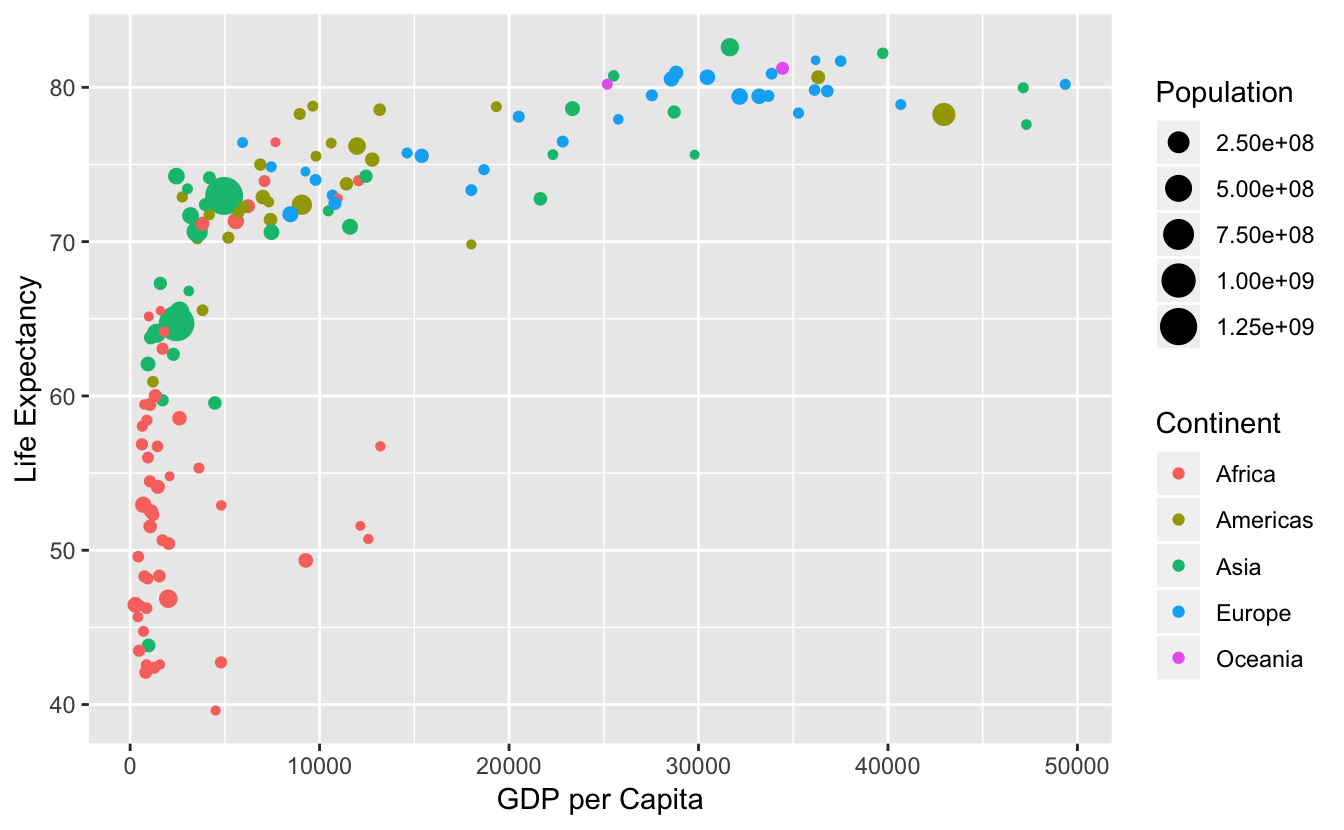
\includegraphics[width=0.9\linewidth]{figure/gapmind-1} 

}

\caption{Espérance de vie en fonction du PIB par habitant en 2007}\label{fig:gapmind}
\end{figure}

Si on décrypte ce graphique du point de vue de la grammaire des
graphiques, on voit que :

\begin{itemize}
\tightlist
\item
  la variable \texttt{GDP\ per\ Capita} est associée à
  l'\texttt{aes}thetic \texttt{x} de la position des points
\item
  la variable \texttt{Life\ Expectancy} est associée à
  l'\texttt{aes}thetic \texttt{y} de la position des points
\item
  la variable \texttt{Population} est associée à l'\texttt{aes}thetic
  \texttt{size} (taille) des points
\item
  la variable \texttt{Continent} est associée à l'\texttt{aes}thetic
  \texttt{color} (couleur) des points
\end{itemize}

Ici, l'objet géométrique (ou \texttt{geom}) qui représente les données
est le point. Les données (ou \texttt{data}) sont contenues dans le
tableau \texttt{gapminder} et chacune de ces variables est associée
(\texttt{mapping}) aux caractéristiques esthétiques des points.

\hypertarget{autres-elements-de-la-grammaire-des-graphiques}{%
\subsubsection{Autres éléments de la grammaire des
graphiques}\label{autres-elements-de-la-grammaire-des-graphiques}}

Outre les éléments indispensables évoqués ici (\texttt{data},
\texttt{mapping}, \texttt{aes}, et \texttt{geom}), il existe d'autres
aspects de la grammaire des graphiques qui permettent de contrôler
l'aspect des graphiques. Ils ne sont pas toujours indispensables. Nous
en verrons néanmoins quelque-uns particulièrement utiles :

\begin{itemize}
\tightlist
\item
  \texttt{facet} : c'est un moyen très pratique de scinder le jeu de
  données en plusieurs sous-groupes et de produire automatiquement un
  graphique pour chacun d'entre eux.
\item
  \texttt{position} : permet notamment de modifier la position des
  barres d'un barplot.
\item
  \texttt{labs} : permet de définir les titres, sous-titres et légendes
  des axes d'un graphique
\item
  \texttt{theme} : permet de modifier l'apect général des graphiques en
  appliquant des thèmes prédéfinis ou en modifiant certains aspects de
  thèmes existants
\end{itemize}

\hypertarget{le-package-ggplot2}{%
\subsubsection{\texorpdfstring{Le package
\texttt{ggplot2}}{Le package ggplot2}}\label{le-package-ggplot2}}

Comme indiqué plus haut, le package \texttt{ggplot2} (Wickham et al.
\protect\hyperlink{ref-R-ggplot2}{2018}) permet de réaliser des
graphiques dans R en respectant les principes de la grammaire des
graphiques. Vous avez probablement remarqué que depuis le début de la
section \ref{gggraph}, beaucoup de termes sont écrits dans la police
réservée au \texttt{code} informatique. C'est parce que les éléments de
la grammaire des graphiques sont tous précisés dans la fonction
\texttt{ggplot()} qui demande, au grand minimum, que les éléments
suivants soient spécifiés :

\begin{itemize}
\tightlist
\item
  le nom du \texttt{data.frame} contenant les variables qui seront
  utilisées pour le graphique. Ce nom correspond à l'argument
  \texttt{data} de la fonction \texttt{ggplot()}.
\item
  l'association des variables à des attributs esthétiques. Cela se fait
  grâce à l'argument \texttt{mapping} et la fonction \texttt{aes()}
\end{itemize}

Après avoir spécifié ces éléments, on ajoute des couches supplémentaires
au graphique grâce au signe \texttt{+}. La couche la plus essentielle à
ajouter à un graphique, est une couche contenant un élément géométrique,
ou \texttt{geom} (par exemple des points, des lignes ou des barres).
D'autres couches peuvent s'ajouter pour spécifier des titres, des
\texttt{facet}s ou des modifications des axes et des thèmes du
graphique.

Dans le cadre de ce cours, nous nous limiterons aux 5 types de
graphiques suivants :

\begin{enumerate}
\def\labelenumi{\arabic{enumi}.}
\tightlist
\item
  les nuages de points
\item
  les graphiques en lignes
\item
  les boîtes à moustaches ou boxplots
\item
  les histogrammes
\item
  les diagrammes bâtons
\end{enumerate}

\begin{center}\rule{0.5\linewidth}{\linethickness}\end{center}

\hypertarget{clouds}{%
\subsection{Les nuages de points}\label{clouds}}

C'est probablement le plus simple des 5 types de graphiques cités plus
haut. Il s'agit de graphiques bi-variés pour lesquels une variable est
associée à l'axe des abscisses, et une autre est associée à l'axe des
ordonnées. Comme pour le graphique présenté à la figure
\ref{fig:gapmind} ci-dessus, d'autres variables peuvent être associées à
des caractéristiques esthétiques des points (transparence, taille,
couleur, forme\ldots{}).

Nous allons ici nous intéresser à la relation qui existe entre :

\begin{enumerate}
\def\labelenumi{\arabic{enumi}.}
\tightlist
\item
  \texttt{dep\_delay} : le retard des vols au décollage, que nous
  placerons sur l'axe des ``x''
\item
  \texttt{arr\_delay} : le retard des mêmes vols à l'aterrissage, que
  nous placerons sur l'axe des ``y''
\end{enumerate}

Afin d'avoir un jeu de données plus facile à utiliser, nous nous
contenterons de visualiser les vols d'Alaska Airlines, donc le code de
compagnie aérienne est \texttt{"AS"}.

\begin{Shaded}
\begin{Highlighting}[]
\NormalTok{alaska_flights <-}\StringTok{ }\NormalTok{flights }\OperatorTok
\StringTok{  }\KeywordTok{filter}\NormalTok{(carrier }\OperatorTok{==}\StringTok{ "AS"}\NormalTok{)}
\end{Highlighting}
\end{Shaded}

Il est normal que vous ne compreniez pas encore les commandes ci-dessus
: elles seront décrites dans le chapitre \ref{wrangling}. Retenez juste
que nous avons créé un nouveau tableau, nommé \texttt{alaska\_flights},
qui contient toutes les informations des vols d'Alaska Airlines.
Commencez par examiner ce tableau avec la fonction \texttt{View()}. En
quoi est-il différent du tableau \texttt{flights} ?

\hypertarget{la-couche-de-base-la-fonction-ggplot}{%
\subsubsection{\texorpdfstring{La couche de base : la fonction
\texttt{ggplot()}}{La couche de base : la fonction ggplot()}}\label{la-couche-de-base-la-fonction-ggplot}}

La fonction \texttt{ggplot()} permet d'établir la première base du
graphique. C'est grâce à cette fonction que l'on précise quel jeu de
données utiliser et quelle variables placer sur les axes :

\begin{Shaded}
\begin{Highlighting}[]
\KeywordTok{ggplot}\NormalTok{(}\DataTypeTok{data =}\NormalTok{ alaska_flights, }\DataTypeTok{mapping =} \KeywordTok{aes}\NormalTok{(}\DataTypeTok{x =}\NormalTok{ dep_delay, }\DataTypeTok{y =}\NormalTok{ arr_delay))}
\end{Highlighting}
\end{Shaded}

\begin{figure}[htpb]

{\centering 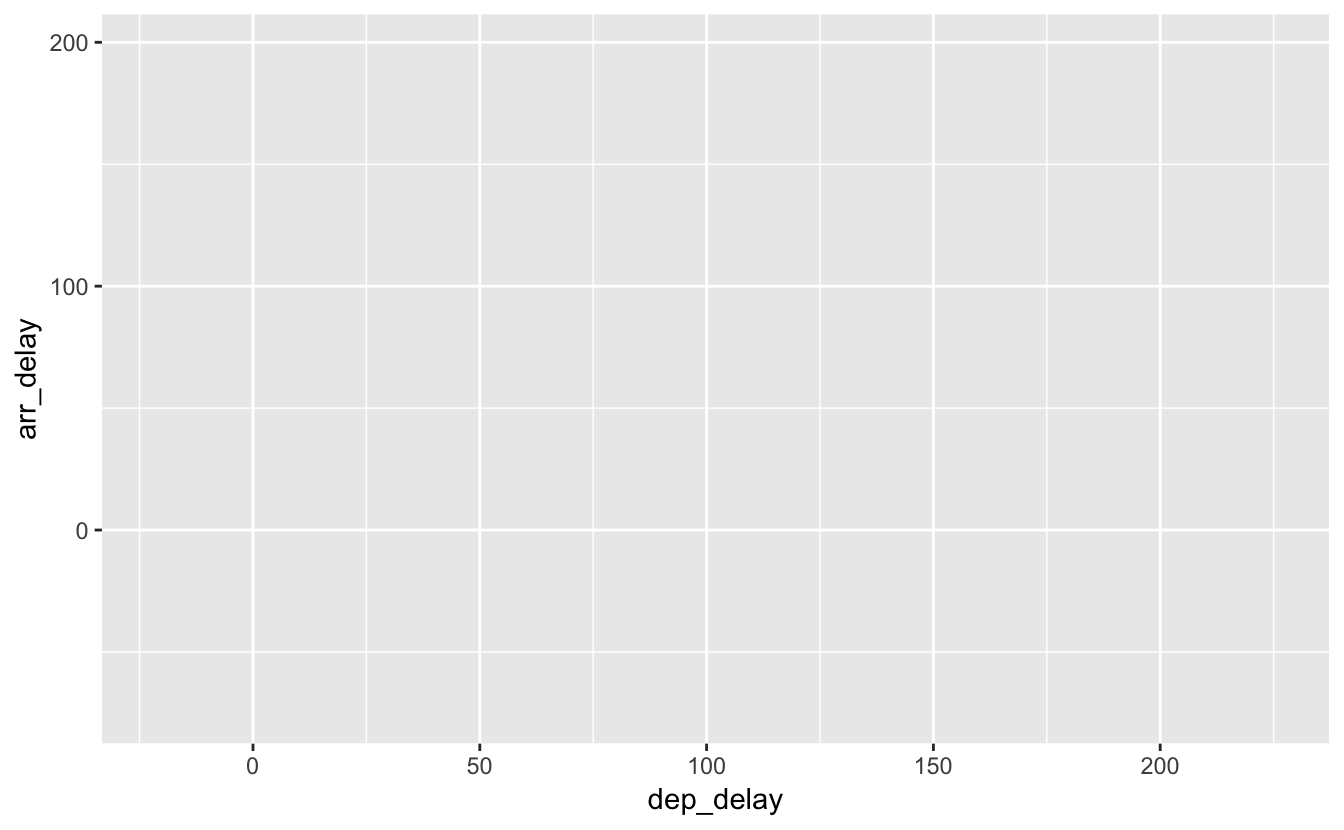
\includegraphics[width=0.9\linewidth]{figure/unnamed-chunk-37-1} 

}

\caption{Un graphique sans `geom`}\label{fig:unnamed-chunk-37}
\end{figure}

Ce graphique est pour le moins vide : c'est normal, nous n'avons pas
encore spécifié la couche contenant l'objet géométrique que nous
souhaitons utiliser.

\hypertarget{ajout-dune-couche-supplementaire-lobjet-geometrique}{%
\subsubsection{Ajout d'une couche supplémentaire : l'objet
géométrique}\label{ajout-dune-couche-supplementaire-lobjet-geometrique}}

Les nuages de points sont créés par la fonction \texttt{geom\_point()} :

\begin{Shaded}
\begin{Highlighting}[]
\KeywordTok{ggplot}\NormalTok{(}\DataTypeTok{data =}\NormalTok{ alaska_flights, }\DataTypeTok{mapping =} \KeywordTok{aes}\NormalTok{(}\DataTypeTok{x =}\NormalTok{ dep_delay, }\DataTypeTok{y =}\NormalTok{ arr_delay)) }\OperatorTok{+}\StringTok{ }
\StringTok{  }\KeywordTok{geom_point}\NormalTok{()}
\end{Highlighting}
\end{Shaded}

\begin{verbatim}
Warning: Removed 5 rows containing missing values (geom_point).
\end{verbatim}

\begin{figure}[htpb]

{\centering 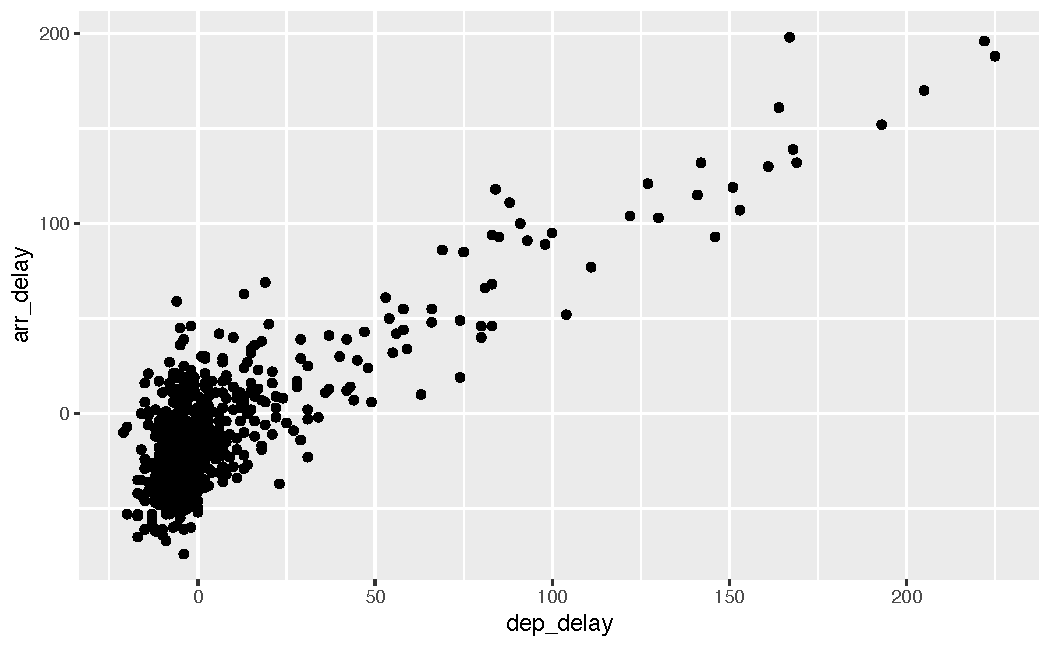
\includegraphics[width=0.9\linewidth]{figure/unnamed-chunk-38-1} 

}

\caption{Retards à l'arrivée en fonction des retard au décollage pour les vols d'Alaska Airline au départ de New York City en 2013}\label{fig:unnamed-chunk-38}
\end{figure}

Plusieurs choses importantes sont à remarquer ici :

\begin{enumerate}
\def\labelenumi{\arabic{enumi}.}
\tightlist
\item
  le graphique présente maintenant une couche supplémentaire constituée
  de points.
\item
  la fonction \texttt{geom\_point()} nous prévient que 5 lignes
  contenant des données manquantes n'ont pas été intégrées au graphique.
  Les données manquent soit pour une variable, soit pour l'autre, soit
  pour les 2. Il est donc impossible de les faire apparaître sur le
  graphique.
\item
  il existe une relation positive entre \texttt{dep\_delay} et
  \texttt{arr\_delay} : quand le retard d'un vol au décollage augmente,
  le retard de ce vol augmente aussi à l'arrivée.
\item
  Enfin, il y a une grande majorité de points centrés près de l'origine
  (0,0).
\end{enumerate}

Si je résume cette syntaxe :

\begin{itemize}
\tightlist
\item
  Au sein de la fonction \texttt{ggplot()}, on spécifie 2 composants de
  la grammaire des graphiques :

  \begin{enumerate}
  \def\labelenumi{\arabic{enumi}.}
  \tightlist
  \item
    le nom du tableau contenant les données grâce à l'argument
    \texttt{data\ =\ alaska\_flights}
  \item
    l'association (\texttt{mapping}) des variables à des
    caractéristiques esthétiques (\texttt{aes()}) en précisant
    \texttt{aes(x\ =\ dep\_delay,\ y\ =\ arr\_delay)} :

    \begin{itemize}
    \tightlist
    \item
      la variable \texttt{dep\_delay} est associée à l'esthétique de
      position \texttt{x}
    \item
      la variable \texttt{arr\_delay} est associée à l'esthétique de
      position \texttt{y}
    \end{itemize}
  \end{enumerate}
\item
  On ajoute une couche au graphique \texttt{ggplot()} grâce au symbole
  \texttt{+}. La couche en question précise le troisème élément
  indispensable de la grammaire des graphiques : l'objet
  \texttt{geom}étrique. Ici, les objets sont des \texttt{point}s. On le
  spécifie grâce à la fonction \texttt{geom\_point()}.
\end{itemize}

Quelques remarques concernant les couches :

\begin{itemize}
\tightlist
\item
  Notez que le signe \texttt{+} est placé \emph{à la fin de la ligne}.
  Vous recevrez un message d'erreur si vous le placez au début.
\item
  Quand vous ajoutez une couche à un graphique, je vous encourage
  vivement à presser la touche \texttt{enter} de votre clavier juste
  après le symbole \texttt{+}. Ainsi, le code correspondant à chaque
  couche sera sur une ligne distincte, ce qui augmente considérablement
  la lisibilité de votre code.
\item
  Comme indiqué dans la section \ref{functions}, tant que les arguments
  d'une fonction sont spécifiés dans l'ordre, on peut se passer d'écrire
  leur nom. Ainsi, les deux blocs de commande suivants produisent
  exactement le même résultat :
\end{itemize}

\begin{Shaded}
\begin{Highlighting}[]
\CommentTok{# Le nom des arguments est précisé}
\KeywordTok{ggplot}\NormalTok{(}\DataTypeTok{data =}\NormalTok{ alaska_flights, }\DataTypeTok{mapping =} \KeywordTok{aes}\NormalTok{(}\DataTypeTok{x =}\NormalTok{ dep_delay, }\DataTypeTok{y =}\NormalTok{ arr_delay)) }\OperatorTok{+}\StringTok{ }
\StringTok{  }\KeywordTok{geom_point}\NormalTok{()}

\CommentTok{# Le nom des arguments est omis}
\KeywordTok{ggplot}\NormalTok{(alaska_flights, }\KeywordTok{aes}\NormalTok{(}\DataTypeTok{x =}\NormalTok{ dep_delay, }\DataTypeTok{y =}\NormalTok{ arr_delay)) }\OperatorTok{+}\StringTok{ }
\StringTok{  }\KeywordTok{geom_point}\NormalTok{()}
\end{Highlighting}
\end{Shaded}

\hypertarget{exercices-2}{%
\subsubsection{Exercices}\label{exercices-2}}

\begin{enumerate}
\def\labelenumi{\arabic{enumi}.}
\tightlist
\item
  Donnez une raison pratique expliquant pourquoi les variables
  \texttt{dep\_delay} et \texttt{arr\_delay} ont une relation positive
\item
  Quelles variables (pas nécessairement dans le tableau
  \texttt{alaska\_flights}) pourraient avoir une corrélation négative
  (relation négative) avec \texttt{dep\_delay} ? Pourquoi ?
  Rappelez-vous que nous étudions ici des variables numériques.
\item
  Selon vous, pourquoi tant de points sont-il regroupés près de (0, 0) ?
  À quoi le point (0,0) correspond-il pour les vols d'Alaska Airline ?
\item
  Citez les éléments de ce graphique/de ces données qui vous sautent le
  plus aux yeux ?
\item
  Créez un nouveau nuage de points en utilisant d'autres variables du
  jeu de données \texttt{alaska\_flights}
\end{enumerate}

\hypertarget{over-plotting}{%
\subsubsection{Over-plotting}\label{over-plotting}}

L'over-plotting est la superposition importante d'une grande quantité
d'information sur une zone restreinte d'un graphique. Dans notre cas,
nous observons un over-plotting important autour de (0,0). Cet effet est
gênant car il est difficile de se faire une idée précise du nombre de
points accumulés dans cette zone. La façon la plus simple de régler le
problème est de modifier la transparence grâce à l'argument
\texttt{alpha} de la fonction \texttt{geom\_point()}. Par défaut, cette
valeur est fixée à 1, pour une opacité totale. Une valeur de 0 rend les
points totalement transparents, et donc invisibles. Trouver la bonne
valeur peut demander de tâtonner une peu :

\begin{Shaded}
\begin{Highlighting}[]
\KeywordTok{ggplot}\NormalTok{(}\DataTypeTok{data =}\NormalTok{ alaska_flights, }\DataTypeTok{mapping =} \KeywordTok{aes}\NormalTok{(}\DataTypeTok{x =}\NormalTok{ dep_delay, }\DataTypeTok{y =}\NormalTok{ arr_delay)) }\OperatorTok{+}\StringTok{ }
\StringTok{  }\KeywordTok{geom_point}\NormalTok{(}\DataTypeTok{alpha =} \FloatTok{0.2}\NormalTok{)}
\end{Highlighting}
\end{Shaded}

\begin{figure}[htpb]

{\centering 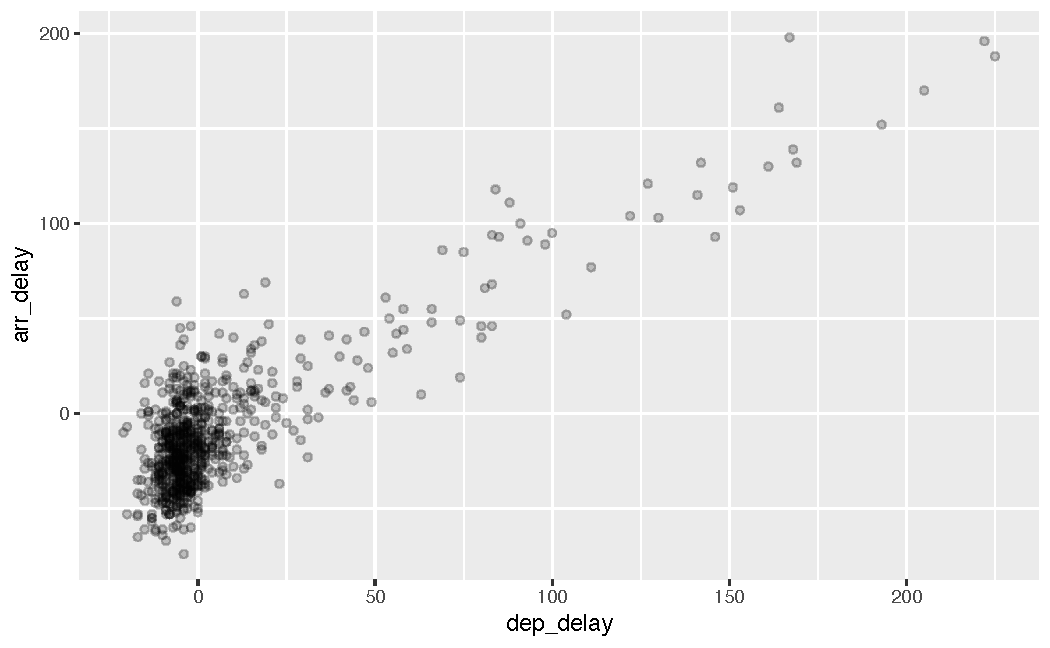
\includegraphics[width=0.9\linewidth]{figure/unnamed-chunk-40-1} 

}

\caption{La même figure, avec des points semi-transparents}\label{fig:unnamed-chunk-40}
\end{figure}

Notez que :

\begin{itemize}
\tightlist
\item
  la transparence est additive : plus il y a de points, plus la zone est
  foncée car les points se superposent et rendent la zone plus opaque.
\item
  l'argument \texttt{alpha\ =\ 0.2} n'est pas intégré à l'intérieur
  d'une fonction \texttt{aes()} car il n'est pas associé à une variable
  : c'est un simple paramètre.
\end{itemize}

L'over-plotting est souvent rencontré lorsque l'on représente plusieurs
nuages de points pour les différentes valeurs d'une variable
catégorielle. par exemple, si on transforme les mois de l'année en
facteur (\texttt{factor(month)}), ont peut regarder s'il existe une
relation entre les retards à l'aterrissage et le mois de l'année :

\begin{Shaded}
\begin{Highlighting}[]
\KeywordTok{ggplot}\NormalTok{(}\DataTypeTok{data =}\NormalTok{ alaska_flights, }\DataTypeTok{mapping =} \KeywordTok{aes}\NormalTok{(}\DataTypeTok{x =} \KeywordTok{factor}\NormalTok{(month), }\DataTypeTok{y =}\NormalTok{ arr_delay)) }\OperatorTok{+}
\StringTok{  }\KeywordTok{geom_point}\NormalTok{()}
\end{Highlighting}
\end{Shaded}

\begin{figure}[htpb]

{\centering 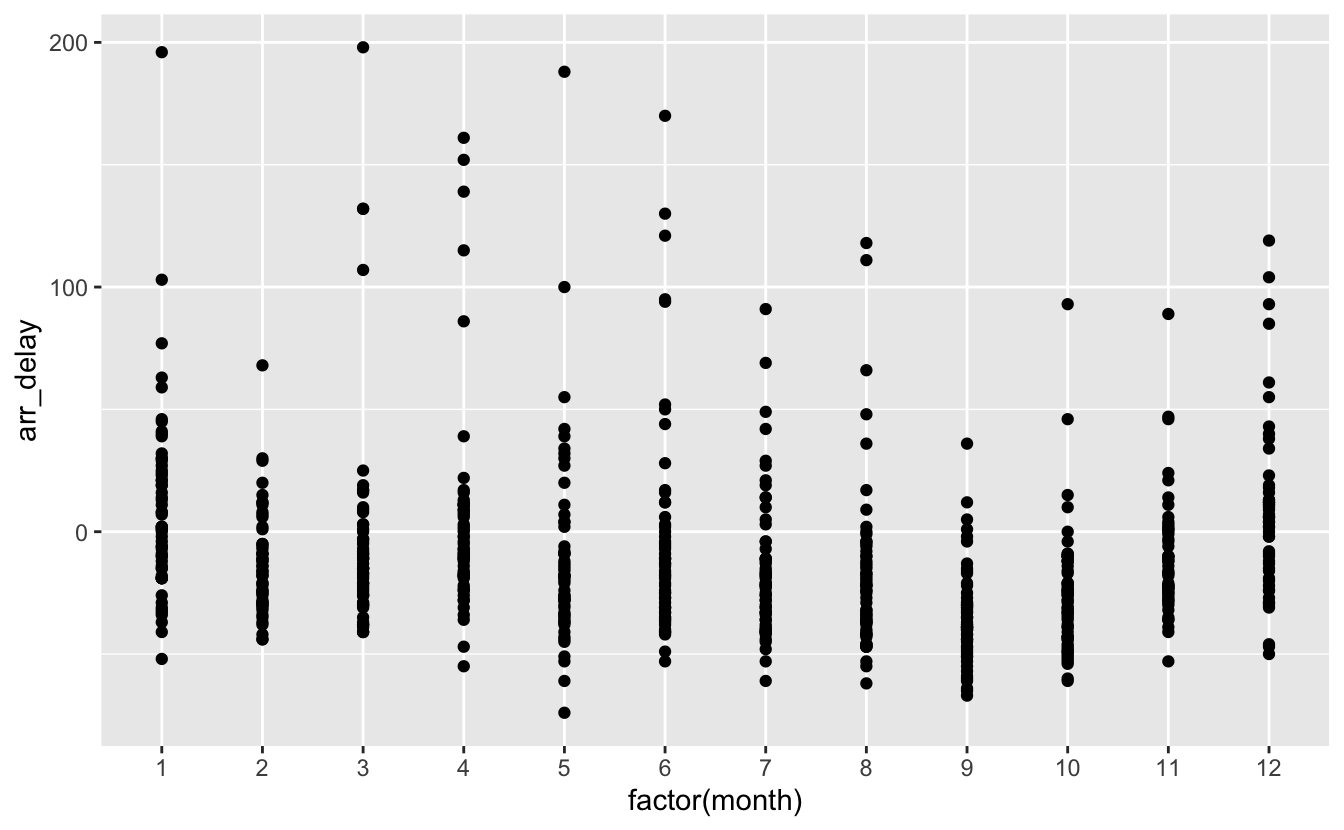
\includegraphics[width=0.9\linewidth]{figure/unnamed-chunk-41-1} 

}

\caption{Retards à l'arrivée pour les 12 mois de l'année 2013}\label{fig:unnamed-chunk-41}
\end{figure}

Ici, l'ajout de transparence ne serait pas suffisant. Une autre solution
est d'appliquer la mothode dîte de ``jittering'', ou tremblement. Elle
consiste à ajouter un bruit aléatoire horizontal et/ou vertical aux
points d'un graphique. Ici, on peut ajouter un léger bruit horizontal
afin de disperser un peu les points pour chaque mois de l'année. On
n'ajoute pas de bruit vertical car on ne souhaite pas que les valeurs de
retard (sur l'axe des \texttt{y}) soient altérées :

\begin{Shaded}
\begin{Highlighting}[]
\KeywordTok{ggplot}\NormalTok{(}\DataTypeTok{data =}\NormalTok{ alaska_flights, }\DataTypeTok{mapping =} \KeywordTok{aes}\NormalTok{(}\DataTypeTok{x =} \KeywordTok{factor}\NormalTok{(month), }\DataTypeTok{y =}\NormalTok{ arr_delay)) }\OperatorTok{+}
\StringTok{  }\KeywordTok{geom_jitter}\NormalTok{(}\DataTypeTok{width =} \FloatTok{0.25}\NormalTok{)}
\end{Highlighting}
\end{Shaded}

\begin{figure}[htpb]

{\centering 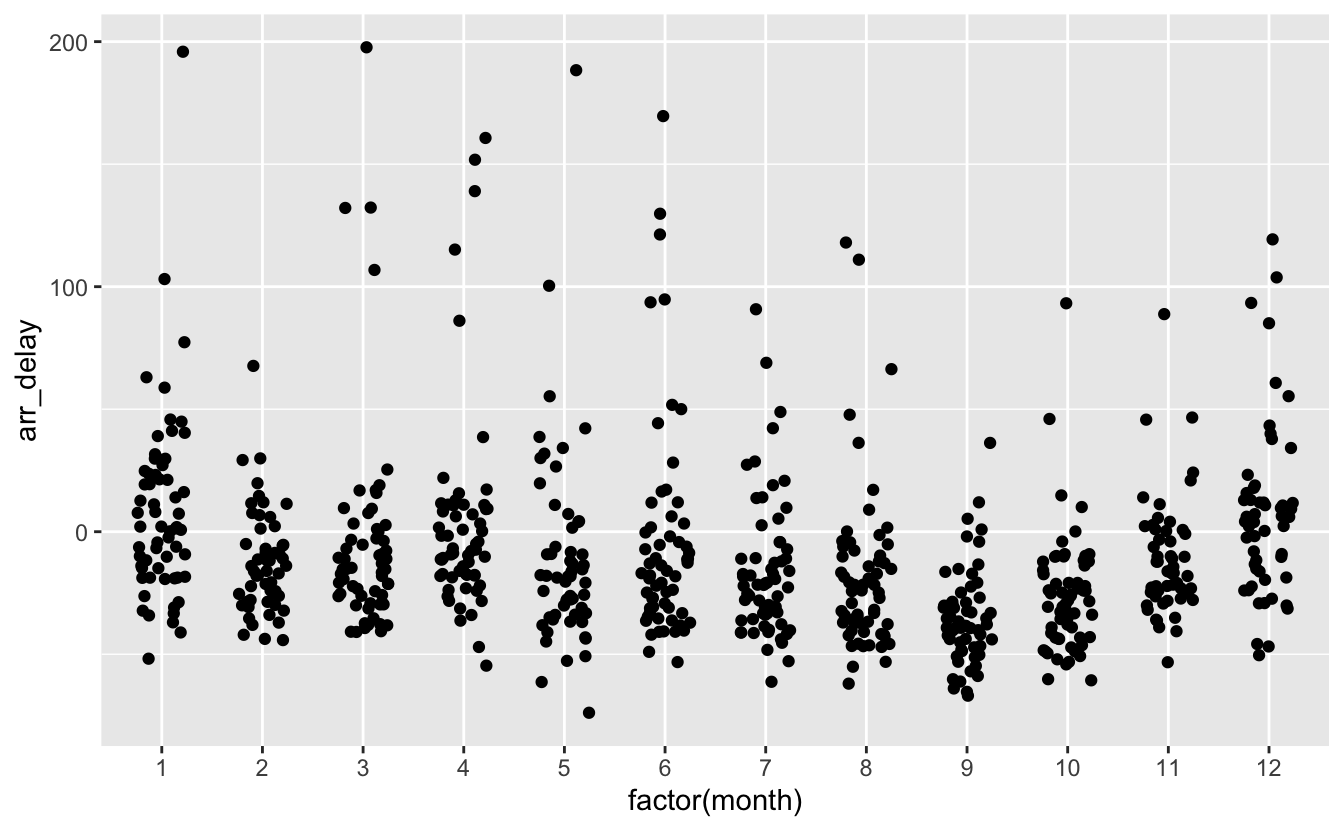
\includegraphics[width=0.9\linewidth]{figure/jittering-1} 

}

\caption{Retards à l'arrivée pour les 12 mois de l'année 2013}\label{fig:jittering}
\end{figure}

On y voit déjà plus clair. L'argument \texttt{width} permet de spécifier
l'intensité de la dispersion horizontale. Pour ajouter du bruit vertical
(ce qui n'est pas souhaitable ici !), on peut ajouter l'argument
\texttt{height}. le graphique de la figure \ref{fig:jittering} est
parfois appelé un ``stripchart''. C'est un graphique du type ``nuage de
points'', mais pour lequel l'une des 2 variables et numérique, et
l'autre est catégorielle.

Il est évidemment possible d'ajouter de la transparence :

\begin{Shaded}
\begin{Highlighting}[]
\KeywordTok{ggplot}\NormalTok{(}\DataTypeTok{data =}\NormalTok{ alaska_flights, }\DataTypeTok{mapping =} \KeywordTok{aes}\NormalTok{(}\DataTypeTok{x =} \KeywordTok{factor}\NormalTok{(month), }\DataTypeTok{y =}\NormalTok{ arr_delay)) }\OperatorTok{+}
\StringTok{  }\KeywordTok{geom_jitter}\NormalTok{(}\DataTypeTok{width =} \FloatTok{0.25}\NormalTok{, }\DataTypeTok{alpha =} \FloatTok{0.5}\NormalTok{)}
\end{Highlighting}
\end{Shaded}

\begin{figure}[htpb]

{\centering 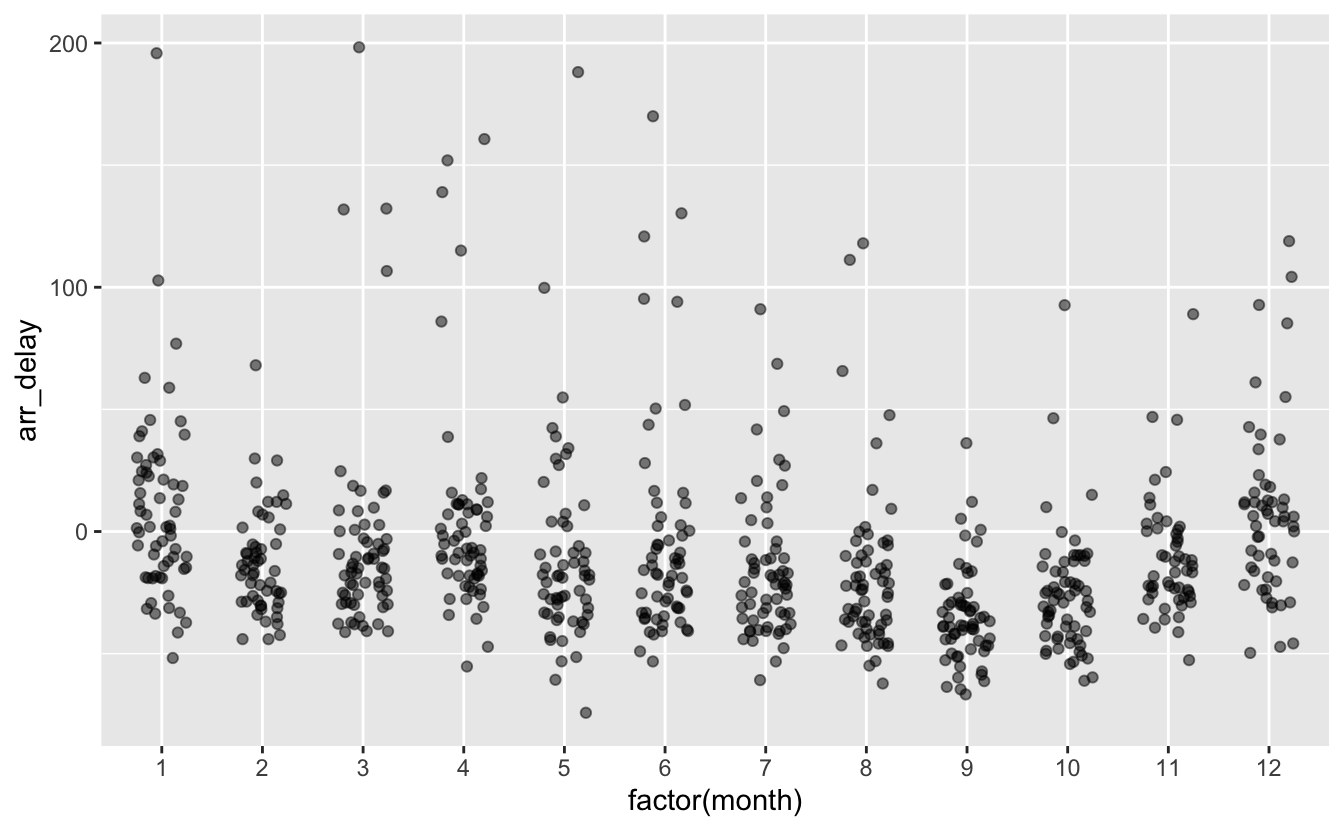
\includegraphics[width=0.9\linewidth]{figure/unnamed-chunk-42-1} 

}

\caption{Retards à l'arrivée pour les 12 mois de l'année 2013}\label{fig:unnamed-chunk-42}
\end{figure}

\hypertarget{couleur-taille-et-forme}{%
\subsubsection{Couleur, taille et forme}\label{couleur-taille-et-forme}}

L'argument \texttt{color} (ou \texttt{colour}, les deux orthographes
fonctionnent) permet de spécifier la couleur des points. L'argument
\texttt{size} permet de spécifier la taille des points. L'argument
\texttt{shape} permet de spécifier la forme utilisée en guise de
symbole. Ces 3 arguments peuvent être utilisés comme des paramètres,
pour modifier l'ensemble des points d'un graphique. Mais ils peuvent
aussi être associés à une variable, pour apporter une information
supplémentaire.

Comparez les deux graphiques suivants :

\begin{Shaded}
\begin{Highlighting}[]
\KeywordTok{ggplot}\NormalTok{(}\DataTypeTok{data =}\NormalTok{ alaska_flights, }\DataTypeTok{mapping =} \KeywordTok{aes}\NormalTok{(}\DataTypeTok{x =}\NormalTok{ dep_delay, }\DataTypeTok{y =}\NormalTok{ arr_delay)) }\OperatorTok{+}
\StringTok{  }\KeywordTok{geom_point}\NormalTok{(}\DataTypeTok{color =} \StringTok{"blue"}\NormalTok{)}
\end{Highlighting}
\end{Shaded}

\begin{figure}[htpb]

{\centering 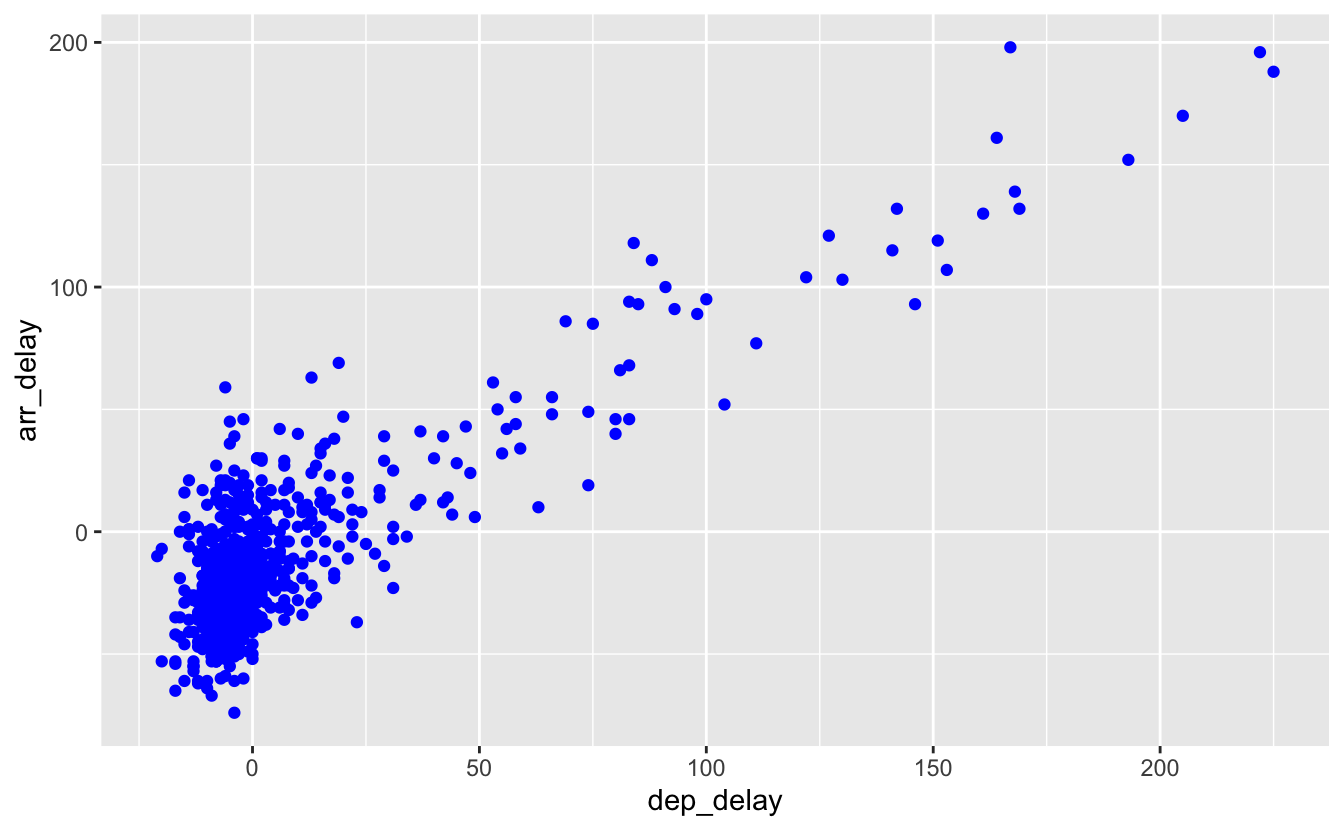
\includegraphics[width=0.9\linewidth]{figure/rightcolor-1} 

}

\caption{Utilisation correcte de `color`}\label{fig:rightcolor}
\end{figure}

\begin{Shaded}
\begin{Highlighting}[]
\KeywordTok{ggplot}\NormalTok{(}\DataTypeTok{data =}\NormalTok{ alaska_flights, }\DataTypeTok{mapping =} \KeywordTok{aes}\NormalTok{(}\DataTypeTok{x =}\NormalTok{ dep_delay, }\DataTypeTok{y =}\NormalTok{ arr_delay)) }\OperatorTok{+}
\StringTok{  }\KeywordTok{geom_point}\NormalTok{(}\KeywordTok{aes}\NormalTok{(}\DataTypeTok{color =} \StringTok{"blue"}\NormalTok{))}
\end{Highlighting}
\end{Shaded}

\begin{figure}[htpb]

{\centering 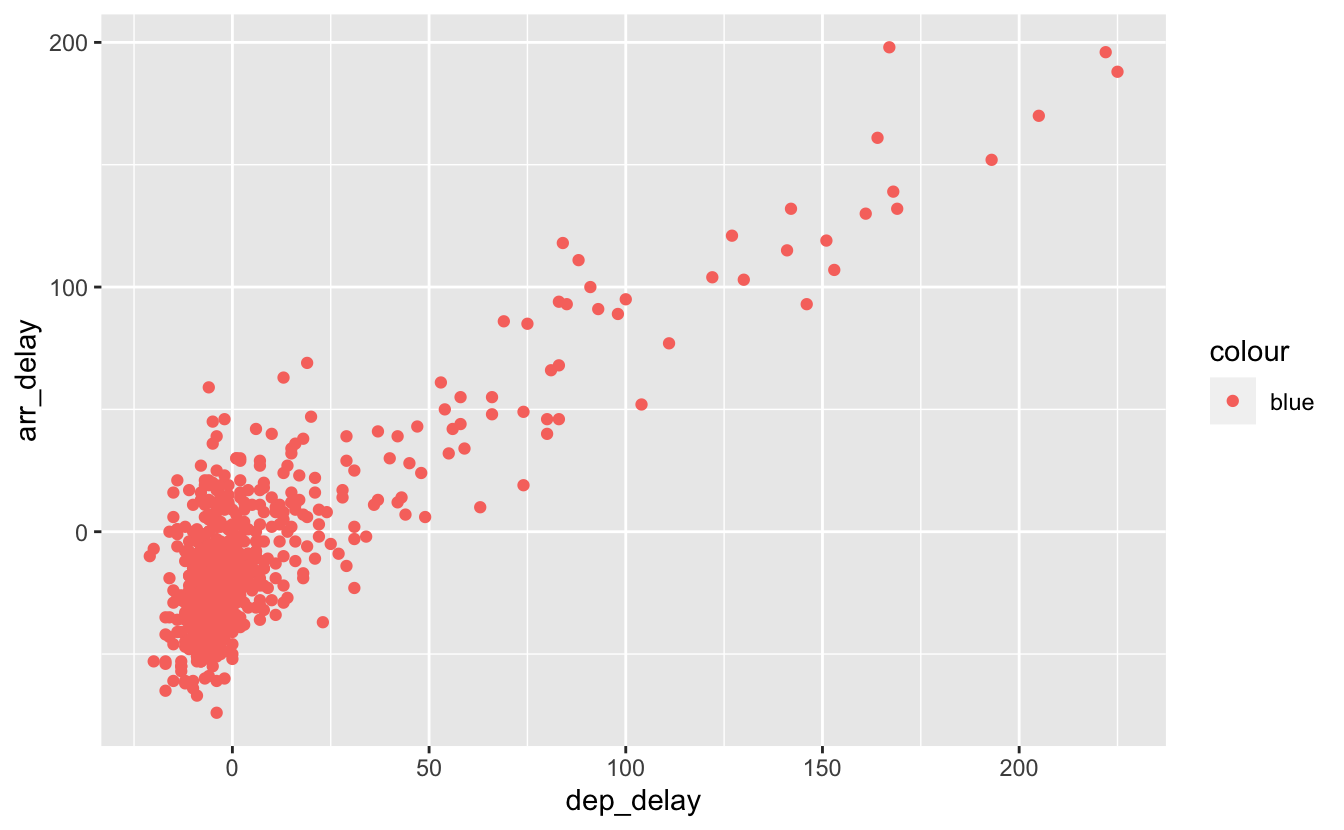
\includegraphics[width=0.9\linewidth]{figure/wrongcolor-1} 

}

\caption{Utilisation incorrecte de `color`}\label{fig:wrongcolor}
\end{figure}

Le code qui permet de produire la figure \ref{fig:rightcolor} fait un
usage correct de l'argument \texttt{color}. On demande des points de
couleur bleue, les points apparaîssent bleus. La figure
\ref{fig:wrongcolor} en revanche ne produit pas le résultat attendu.
Puisque nous avons mis l'argument \texttt{color} à l'intérieur de la
fonction \texttt{aes()}, R s'attend à ce que la couleur soit associée à
une variable. Puisqu'aucune variable ne s'appelle ``blue'', R utilise la
couleur par défaut. Pour associer la couleur des points à une variable,
nous devons fournir un nom de variable valide :

\begin{Shaded}
\begin{Highlighting}[]
\KeywordTok{ggplot}\NormalTok{(}\DataTypeTok{data =}\NormalTok{ alaska_flights, }\DataTypeTok{mapping =} \KeywordTok{aes}\NormalTok{(}\DataTypeTok{x =}\NormalTok{ dep_delay, }\DataTypeTok{y =}\NormalTok{ arr_delay)) }\OperatorTok{+}
\StringTok{  }\KeywordTok{geom_point}\NormalTok{(}\KeywordTok{aes}\NormalTok{(}\DataTypeTok{color =} \KeywordTok{factor}\NormalTok{(month)))}
\end{Highlighting}
\end{Shaded}

\begin{figure}[htpb]

{\centering 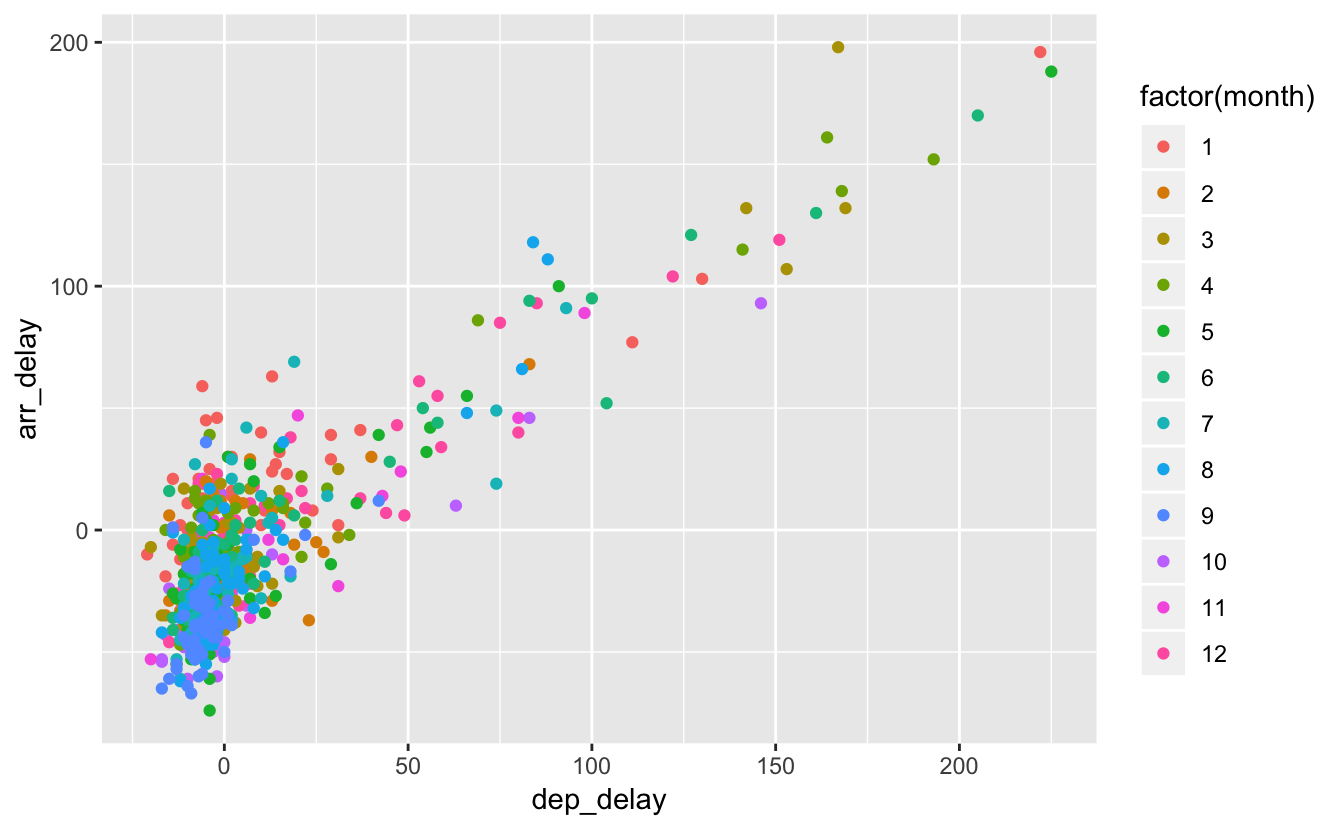
\includegraphics[width=0.9\linewidth]{figure/varcolor-1} 

}

\caption{Association de `color` à une variable catégorielle}\label{fig:varcolor}
\end{figure}

Ici, l'utilisation de la couleur est correcte. Elle est associée à une
variable catégorielle, et chaque valeur possible du vecteur
\texttt{month} se voit donc attribuer une couleur différente.

\begin{Shaded}
\begin{Highlighting}[]
\KeywordTok{ggplot}\NormalTok{(}\DataTypeTok{data =}\NormalTok{ alaska_flights, }\DataTypeTok{mapping =} \KeywordTok{aes}\NormalTok{(}\DataTypeTok{x =}\NormalTok{ dep_delay, }\DataTypeTok{y =}\NormalTok{ arr_delay)) }\OperatorTok{+}
\StringTok{  }\KeywordTok{geom_point}\NormalTok{(}\KeywordTok{aes}\NormalTok{(}\DataTypeTok{color =}\NormalTok{ arr_time))}
\end{Highlighting}
\end{Shaded}

\begin{figure}[htpb]

{\centering 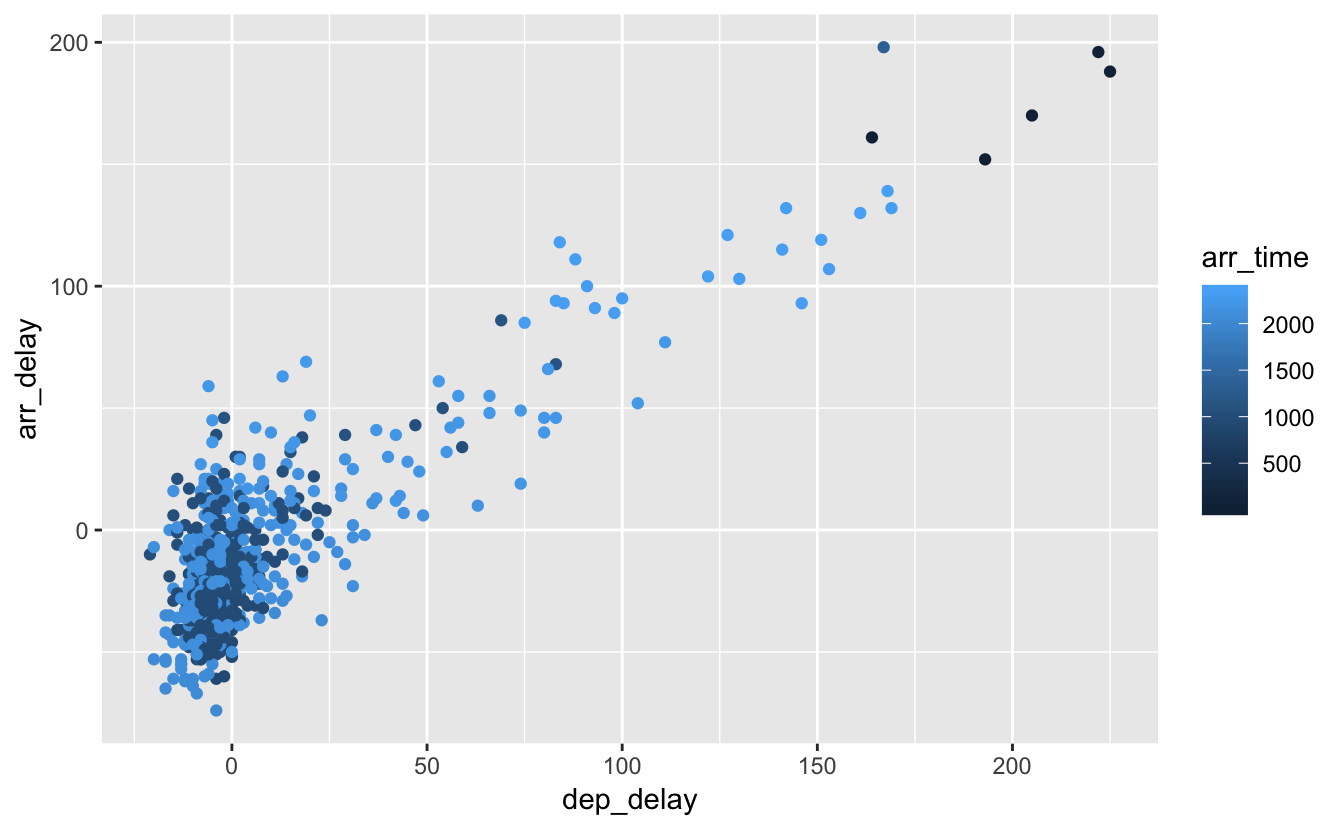
\includegraphics[width=0.9\linewidth]{figure/varcolor2-1} 

}

\caption{Association de `color` à une variable numérique}\label{fig:varcolor2}
\end{figure}

De la même façon, la couleur des points est ici associée à une variable
continue (l'heure d'arrivée des vols). Les points se voient donc
attribuer une couleur choisie le long d'un gradient.

La même approche peut être utilisée pour spécifier la forme des symboles
avec l'argument \texttt{shape}. Attention toutefois : une variable
continue ne peut pas être associée à \texttt{shape}

\begin{Shaded}
\begin{Highlighting}[]
\KeywordTok{ggplot}\NormalTok{(}\DataTypeTok{data =}\NormalTok{ alaska_flights, }\DataTypeTok{mapping =} \KeywordTok{aes}\NormalTok{(}\DataTypeTok{x =}\NormalTok{ dep_delay, }\DataTypeTok{y =}\NormalTok{ arr_delay)) }\OperatorTok{+}
\StringTok{  }\KeywordTok{geom_point}\NormalTok{(}\KeywordTok{aes}\NormalTok{(}\DataTypeTok{shape =} \KeywordTok{factor}\NormalTok{(month)))}
\end{Highlighting}
\end{Shaded}

\begin{figure}[htpb]

{\centering 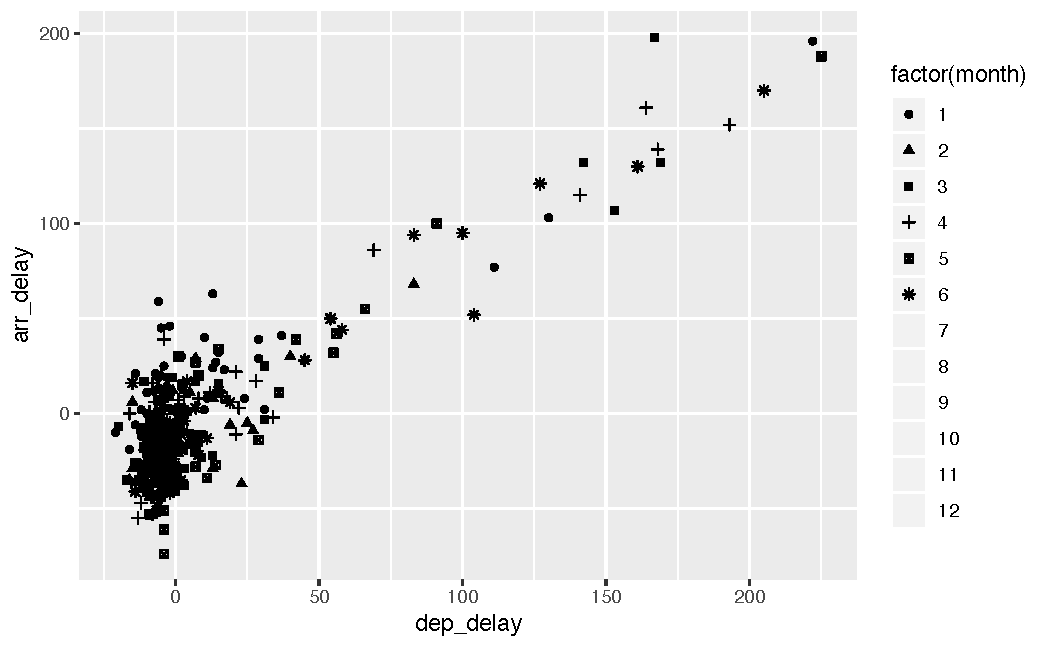
\includegraphics[width=0.9\linewidth]{figure/shapeplot-1} 

}

\caption{Association de `shape` à un facteur}\label{fig:shapeplot}
\end{figure}

Vous noterez que seuls les 6 premiers niveaux d'un facteur se voient
attribuer une forme automatiquement. Au delà de 6 symboles différents
sur un même graphique, le résultat est souvent illisible. Il est
possible d'ajouter plus de 6 symboles, mais cela demande de modifier la
légende manuellement et concrètement nous n'en aurons jamais besoin.
Lorsque plus de 6 séries doivent être distinguées, d'autres solutions
bien plus pertinentes (par exemple les \texttt{factet}s) devraient être
utilisées.

Comme pour la couleur, il est possible d'e spécifier'utiliser l'argument
\texttt{shape} en tant que paramètre du graphique sans l'associer à une
variable. Il faut alors fournir un code compris entre 0 et 24 :

\begin{Shaded}
\begin{Highlighting}[]
\KeywordTok{ggplot}\NormalTok{(}\DataTypeTok{data =}\NormalTok{ alaska_flights, }\DataTypeTok{mapping =} \KeywordTok{aes}\NormalTok{(}\DataTypeTok{x =}\NormalTok{ dep_delay, }\DataTypeTok{y =}\NormalTok{ arr_delay)) }\OperatorTok{+}
\StringTok{  }\KeywordTok{geom_point}\NormalTok{(}\DataTypeTok{shape =} \DecValTok{4}\NormalTok{)}
\end{Highlighting}
\end{Shaded}

\begin{figure}[htpb]

{\centering 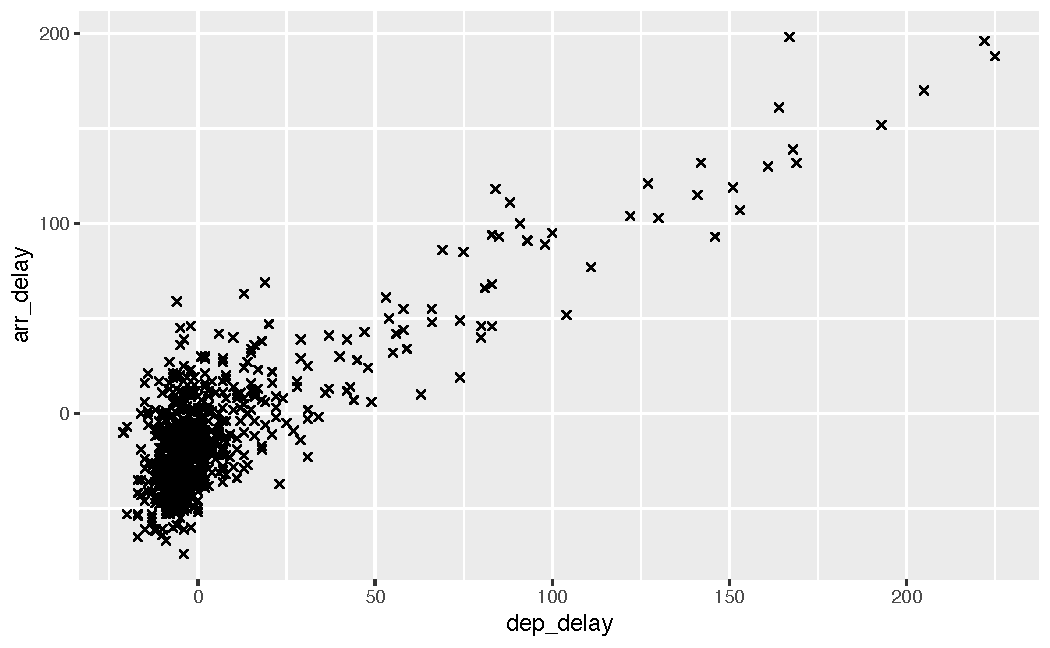
\includegraphics[width=0.9\linewidth]{figure/shapeplot2-1} 

}

\caption{Utilisation de `shape` en tant que paramètre}\label{fig:shapeplot2}
\end{figure}

Notez qu'ici, \texttt{ggplot()} ne crée pas de légende : tous les points
ont le même symbole, ce symbole n'est pas associé à une variable, une
légende est donc inutile.

Parmis les valeur possibles pour \texttt{shape}, les symboles 21 à 24
sont des symboles dont on peut spécifier séparément la couleur du
contour, avec \texttt{color} et la couleur du fond avec \texttt{fill} :

\begin{Shaded}
\begin{Highlighting}[]
\KeywordTok{ggplot}\NormalTok{(}\DataTypeTok{data =}\NormalTok{ alaska_flights, }\DataTypeTok{mapping =} \KeywordTok{aes}\NormalTok{(}\DataTypeTok{x =}\NormalTok{ dep_delay, }\DataTypeTok{y =}\NormalTok{ arr_delay)) }\OperatorTok{+}
\StringTok{  }\KeywordTok{geom_point}\NormalTok{(}\DataTypeTok{shape =} \DecValTok{21}\NormalTok{, }\DataTypeTok{fill =} \StringTok{"steelblue"}\NormalTok{, }\DataTypeTok{color =} \StringTok{"orange"}\NormalTok{, }\DataTypeTok{alpha =} \FloatTok{0.5}\NormalTok{)}
\end{Highlighting}
\end{Shaded}

\begin{figure}[htpb]

{\centering 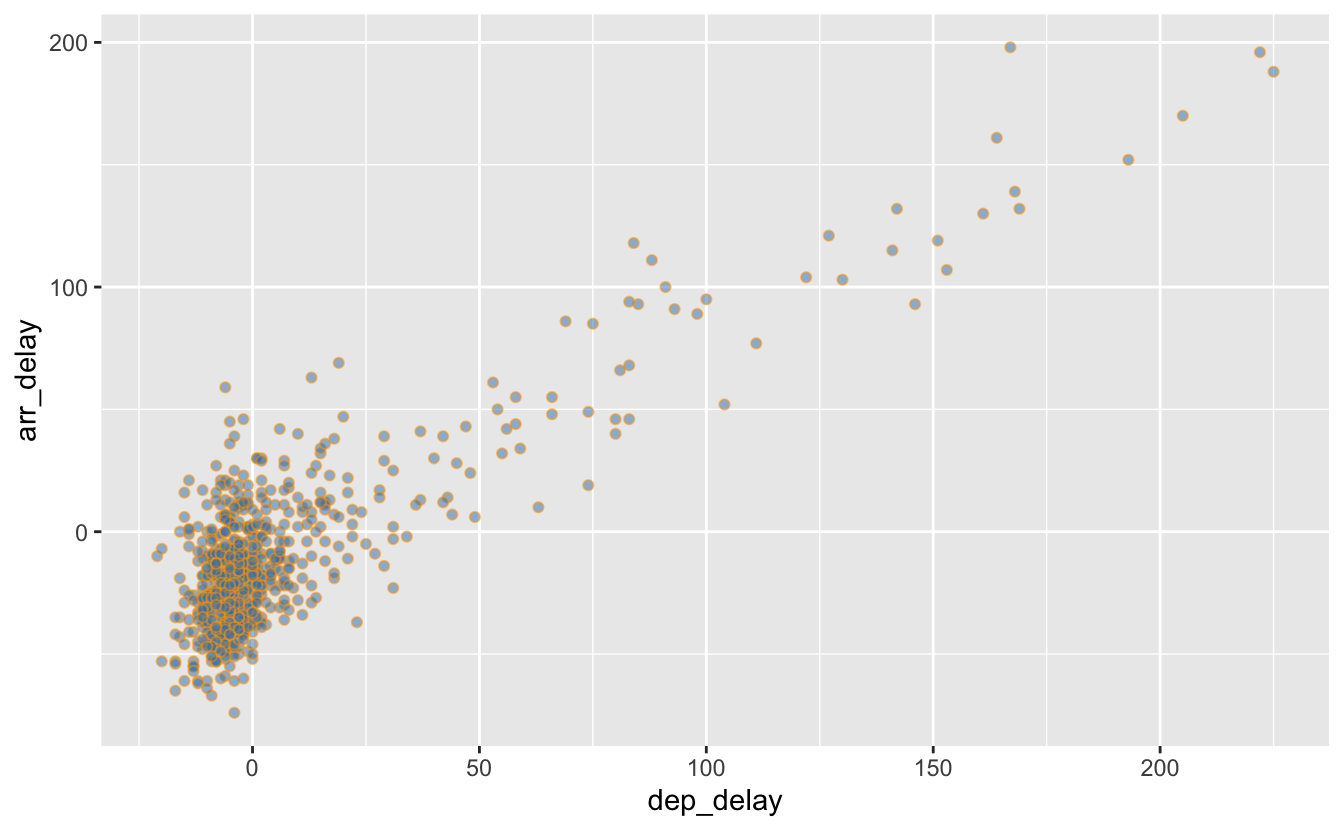
\includegraphics[width=0.9\linewidth]{figure/shapecolorplot-1} 

}

\caption{Utilisation de `shape`, `color` et `fill`}\label{fig:shapecolorplot}
\end{figure}

N'hésitez pas à zoomer pour bien observer les points et comprendre ce
qui se passe. Un conseil, faites des choix raisonnables ! Trop de
couleurs n'est pas forcément souhaitable.

Enfin, on peut ajuster la taille des symboles avec l'argument
\texttt{size}. Tout comme il n'est pas possible d'associer une variable
continue à \texttt{shape}, et il n'est pas conseillé d'associer une
variable catégorielle nominale (c'est à dire un facteur non ordonné) à
\texttt{size}. Associer une variable continue est en ravanche parfois
utile :

\begin{Shaded}
\begin{Highlighting}[]
\KeywordTok{ggplot}\NormalTok{(}\DataTypeTok{data =}\NormalTok{ alaska_flights, }\DataTypeTok{mapping =} \KeywordTok{aes}\NormalTok{(}\DataTypeTok{x =}\NormalTok{ dep_delay, }\DataTypeTok{y =}\NormalTok{ arr_delay)) }\OperatorTok{+}
\StringTok{  }\KeywordTok{geom_point}\NormalTok{(}\KeywordTok{aes}\NormalTok{(}\DataTypeTok{size =}\NormalTok{ arr_time), }\DataTypeTok{alpha =} \FloatTok{0.1}\NormalTok{)}
\end{Highlighting}
\end{Shaded}

\begin{figure}[htpb]

{\centering 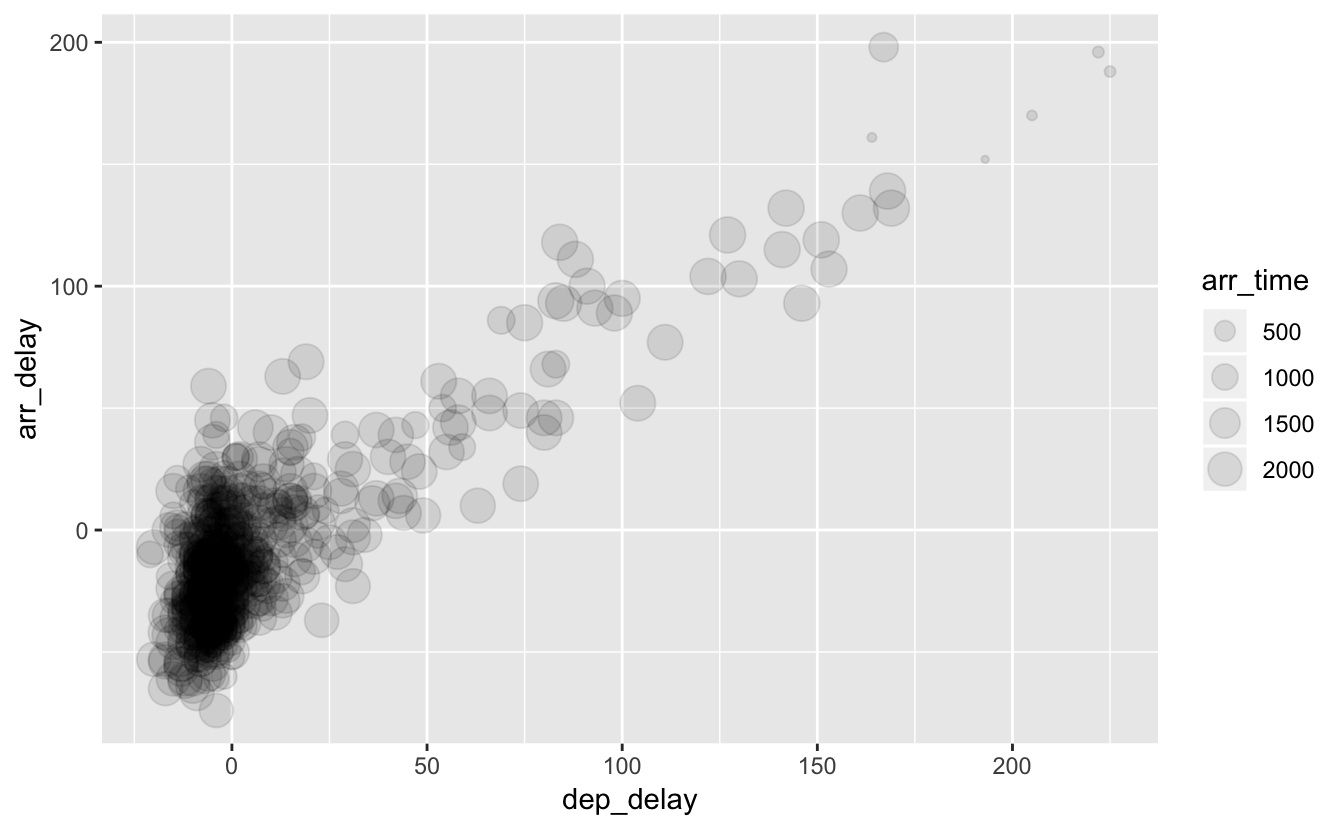
\includegraphics[width=0.9\linewidth]{figure/sizeplot-1} 

}

\caption{Association d'une variable continue à la taille des symboles avec l'argument `size`}\label{fig:sizeplot}
\end{figure}

Si l'over-plotting est ici très important (c'est pourquoi j'ai utilisé
\texttt{alpha}), on constate néanmoins que les vols avec les retards les
plus importants sont presque tous arrivés très tôt dans la journée
(``500'' signifie 5h00 du matin). Il s'agit probablement de vols qui
devaient arriver dans la nuit, avant minuit, et qui sont finalement
arrivés en tout début de journée, etnre 00h01 et 5h00 du matin. Comme
pour les autres arguments, il est possible d'utiliser \texttt{size} avec
une valeur fixe, la même pour tous les symboles, lorsque cet argument
n'est pas associé à une variable.

Enfin un conseil : évitez de trop surcharger vos graphiques. En
combinant l'ensemble de ces arguments, il est malheureusement très
facile d'obtenir des graphiques peu lisibles, ou contenant tellement
d'information qu'ils en deviennent difficiles à déchiffrer. Faites
preuve de modération :

\begin{Shaded}
\begin{Highlighting}[]
\KeywordTok{ggplot}\NormalTok{(}\DataTypeTok{data =}\NormalTok{ alaska_flights, }\DataTypeTok{mapping =} \KeywordTok{aes}\NormalTok{(}\DataTypeTok{x =}\NormalTok{ dep_delay, }\DataTypeTok{y =}\NormalTok{ arr_delay, }\DataTypeTok{size =}\NormalTok{ arr_time)) }\OperatorTok{+}
\StringTok{  }\KeywordTok{geom_point}\NormalTok{(}\DataTypeTok{alpha =} \FloatTok{0.6}\NormalTok{, }
             \DataTypeTok{shape =} \DecValTok{22}\NormalTok{,}
             \DataTypeTok{color =} \StringTok{"orange"}\NormalTok{,}
             \DataTypeTok{fill =} \StringTok{"steelblue"}\NormalTok{,}
             \DataTypeTok{stroke =} \DecValTok{2}\NormalTok{)}
\end{Highlighting}
\end{Shaded}

\begin{figure}[htpb]

{\centering 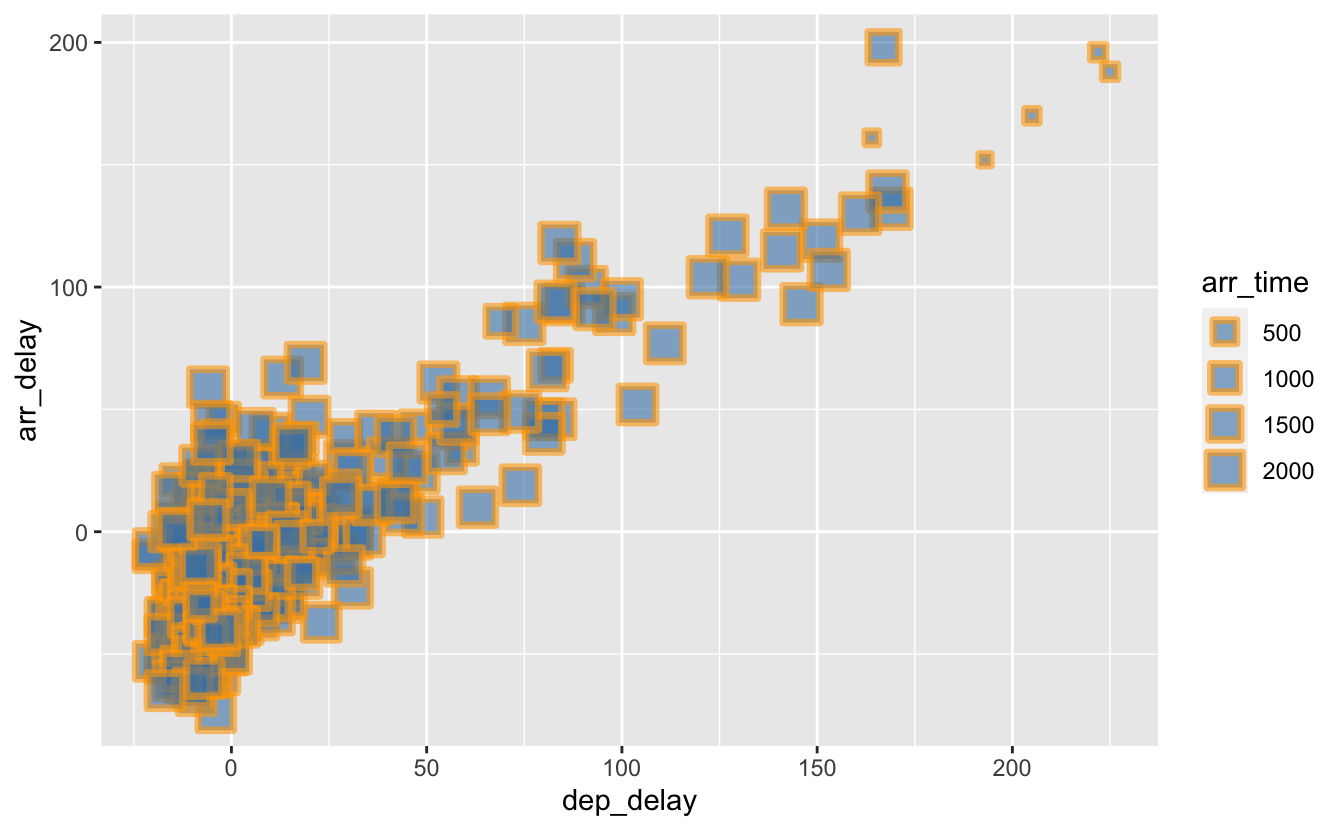
\includegraphics[width=0.9\linewidth]{figure/badplot-1} 

}

\caption{Sometimes, less is more!}\label{fig:badplot}
\end{figure}

\hypertarget{exercices-3}{%
\subsubsection{Exercices}\label{exercices-3}}

À quoi sert l'argument \texttt{stroke} ?

Avec le jeu de données \texttt{diamonds}, tapez le code permettant de
créer le graphique \ref{fig:exodiamonds} (Indice : affichez le tableau
\texttt{diamonds} dans la console afin de voir quelles sont les
variables disponibles).

\begin{figure}[htpb]

{\centering 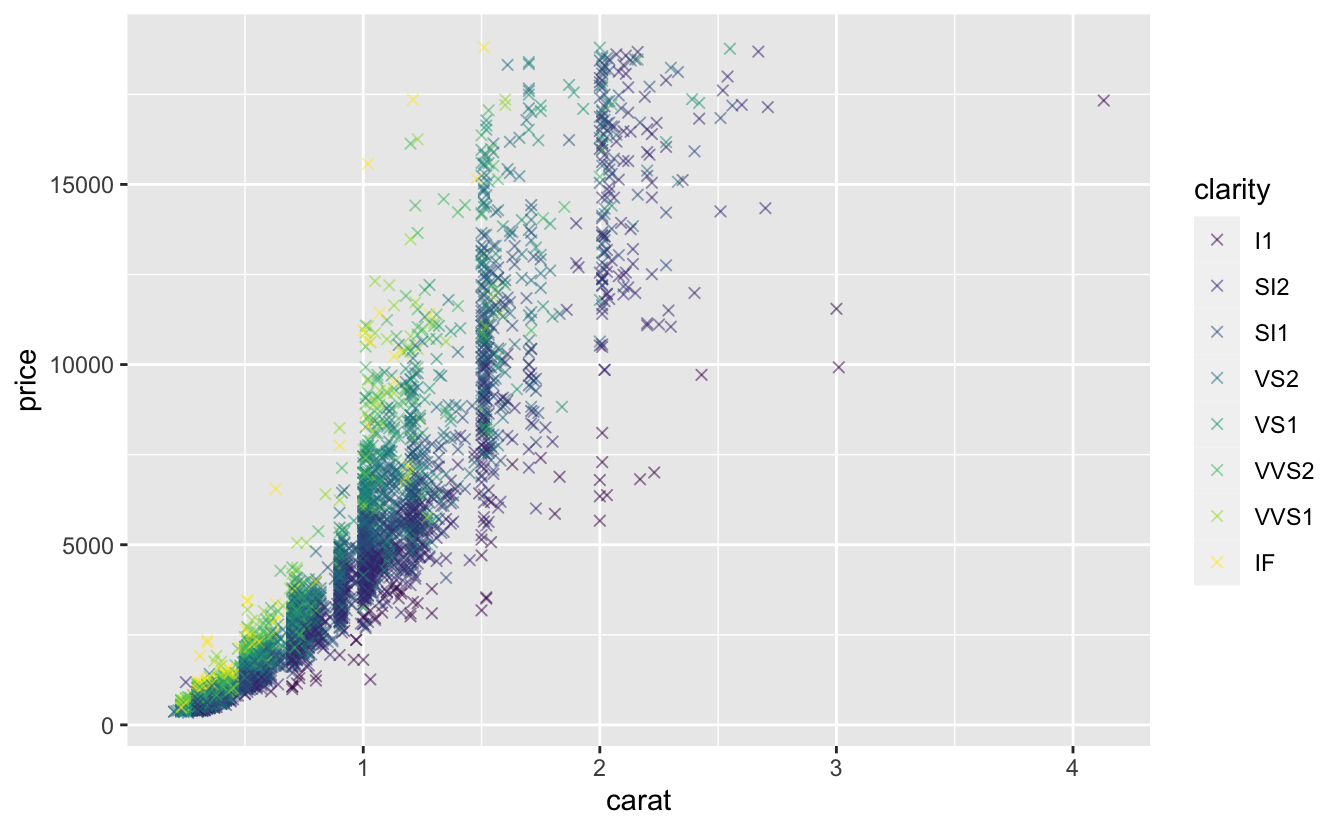
\includegraphics[width=0.9\linewidth]{figure/exodiamonds-1} 

}

\caption{Prix de 53940 diamants en fonction de leur taille en carats et de leur couleur.}\label{fig:exodiamonds}
\end{figure}

Selon vous, à quoi sont dues les bandes verticales que l'on observe sur
ce graphique ?

\begin{center}\rule{0.5\linewidth}{\linethickness}\end{center}

\hypertarget{les-graphiques-en-lignes}{%
\subsection{Les graphiques en lignes}\label{les-graphiques-en-lignes}}

\hypertarget{un-nouveau-jeu-de-donnees}{%
\subsubsection{Un nouveau jeu de
données}\label{un-nouveau-jeu-de-donnees}}

Les graphiques en ligne, ou ``linegraphs'' sont généralement utilisés
lorsque l'axe des \texttt{x} porte une information \textbf{temporelle},
et l'axe des \texttt{y} une autre variable numérique. Le temps est une
variable naturellement ordonnée : les jours, semaines, mois, années, se
suivent naturellement. Les graphiques en lignes devraient être évités
lorsqu'il n'y a pas une organisation séquentielle évidente de la
variable portée par l'axe des \texttt{x}.

Concentrons nous maintenant sur le tableau \texttt{weather} du package
\texttt{nycflights13}. Explorez ce tableau en appliquant les méthodes
vues dans le chapitre \ref{dataset}. N'oubliez pas de consultez l'aide
de ce jeu de données.

\begin{Shaded}
\begin{Highlighting}[]
\NormalTok{weather}
\end{Highlighting}
\end{Shaded}

\begin{verbatim}
# A tibble: 26,115 x 15
   origin  year month   day  hour  temp  dewp humid wind_dir wind_speed
   <chr>  <dbl> <dbl> <int> <int> <dbl> <dbl> <dbl>    <dbl>      <dbl>
 1 EWR     2013     1     1     1  39.0  26.1  59.4      270      10.4 
 2 EWR     2013     1     1     2  39.0  27.0  61.6      250       8.06
 3 EWR     2013     1     1     3  39.0  28.0  64.4      240      11.5 
 4 EWR     2013     1     1     4  39.9  28.0  62.2      250      12.7 
 5 EWR     2013     1     1     5  39.0  28.0  64.4      260      12.7 
 6 EWR     2013     1     1     6  37.9  28.0  67.2      240      11.5 
 7 EWR     2013     1     1     7  39.0  28.0  64.4      240      15.0 
 8 EWR     2013     1     1     8  39.9  28.0  62.2      250      10.4 
 9 EWR     2013     1     1     9  39.9  28.0  62.2      260      15.0 
10 EWR     2013     1     1    10  41    28.0  59.6      260      13.8 
# ... with 26,105 more rows, and 5 more variables: wind_gust <dbl>,
#   precip <dbl>, pressure <dbl>, visib <dbl>, time_hour <dttm>
\end{verbatim}

Nous allons nous intéresser à la variable \texttt{temp}, qui contient un
enregistrement de température pour chaque heure de chaque jour de 2013
pour les 3 aéroports de New York. Cela représente une grande quantité de
données, aussi, nous nous limiterons aux températures observées entre le
1er et le 15 janvier, pour l'aéroport Newark uniquement.

\begin{Shaded}
\begin{Highlighting}[]
\NormalTok{small_weather <-}\StringTok{ }\NormalTok{weather }\OperatorTok\StringTok{ }
\StringTok{  }\KeywordTok{filter}\NormalTok{(origin }\OperatorTok{==}\StringTok{ "EWR"}\NormalTok{,}
\NormalTok{         month }\OperatorTok{==}\StringTok{ }\DecValTok{1}\NormalTok{,}
\NormalTok{         day }\OperatorTok{<=}\StringTok{ }\DecValTok{15}\NormalTok{)}
\end{Highlighting}
\end{Shaded}

La fonction \texttt{filter()} fonctionne sur le même principe que la
fonction \texttt{subset()} vue lors du premier TP. Ici, nous demandons à
R de créer un nouveau tableau de données, nommé \texttt{small\_weather},
qui ne contiendra que les lignes correspondant à
\texttt{origin\ ==\ "EWR"}, et \texttt{month\ ==\ 1}, et
\texttt{day\ \textless{}=\ 15}, c'est à dire les données météorologiques
de l'aéroport de Newark pour les 15 premiers jours de janvier 2013.

\hypertarget{exercice}{%
\subsubsection{Exercice}\label{exercice}}

Avec \texttt{View()}, consultez le tableau nouvellement créé. Expliquez
pourquoi la variable \texttt{time\_hour} identifie de manière unique le
moment ou chaque mesure a été réalisée alors que ce n'est pas le cas de
la variable \texttt{hour}.

\hypertarget{la-fonction-geom_line}{%
\subsubsection{\texorpdfstring{La fonction
\texttt{geom\_line()}}{La fonction geom\_line()}}\label{la-fonction-geom_line}}

Les line graphs sont produits de la même façon que les nuages de points.
Seul l'objet géométrique permettant de visualiser les données change. Au
lieu d'utiliser \texttt{geom\_point()}, on utilisera
\texttt{geom\_line()} :

\begin{Shaded}
\begin{Highlighting}[]
\KeywordTok{ggplot}\NormalTok{(}\DataTypeTok{data =}\NormalTok{ small_weather, }\DataTypeTok{mapping =} \KeywordTok{aes}\NormalTok{(}\DataTypeTok{x =}\NormalTok{ time_hour, }\DataTypeTok{y =}\NormalTok{ temp)) }\OperatorTok{+}
\StringTok{  }\KeywordTok{geom_line}\NormalTok{()}
\end{Highlighting}
\end{Shaded}

\begin{figure}[htpb]

{\centering 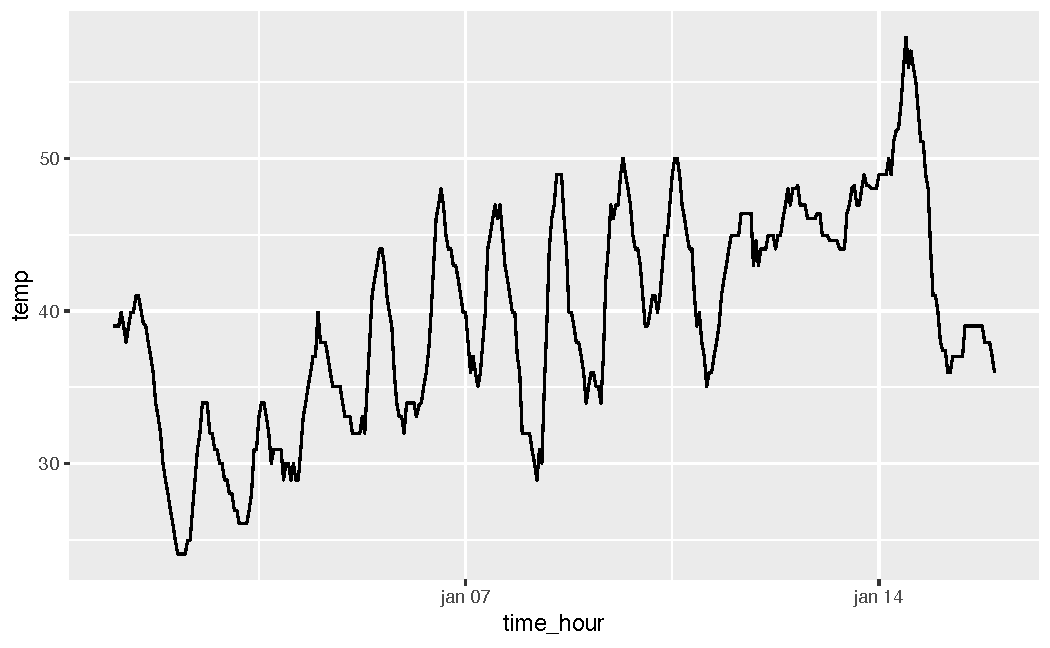
\includegraphics[width=0.9\linewidth]{figure/linegraph-1} 

}

\caption{Températures horaires à l'aéroport de Newark entre le 1er et le 15 janvier 2013}\label{fig:linegraph}
\end{figure}

Très logiquement, on observe des oscillations plus ou moins régulières
qui correspondent à l'alternance jour/nuit. Notez l'échelle de l'axe des
ordonnées : les températures sont enregistrées en degrés Farenheit.

Nous connaissons maintenant 2 types d'objets \texttt{geom}étriques : les
points les les lignes. il est tout à fait possible d'ajouter plusieurs
couches à un graphique, chacune d'elle correspondant à un objet
\texttt{geom}étrique différent :

\begin{Shaded}
\begin{Highlighting}[]
\KeywordTok{ggplot}\NormalTok{(}\DataTypeTok{data =}\NormalTok{ small_weather, }\DataTypeTok{mapping =} \KeywordTok{aes}\NormalTok{(}\DataTypeTok{x =}\NormalTok{ time_hour, }\DataTypeTok{y =}\NormalTok{ temp)) }\OperatorTok{+}
\StringTok{  }\KeywordTok{geom_line}\NormalTok{() }\OperatorTok{+}
\StringTok{  }\KeywordTok{geom_point}\NormalTok{()}
\end{Highlighting}
\end{Shaded}

\begin{figure}[htpb]

{\centering 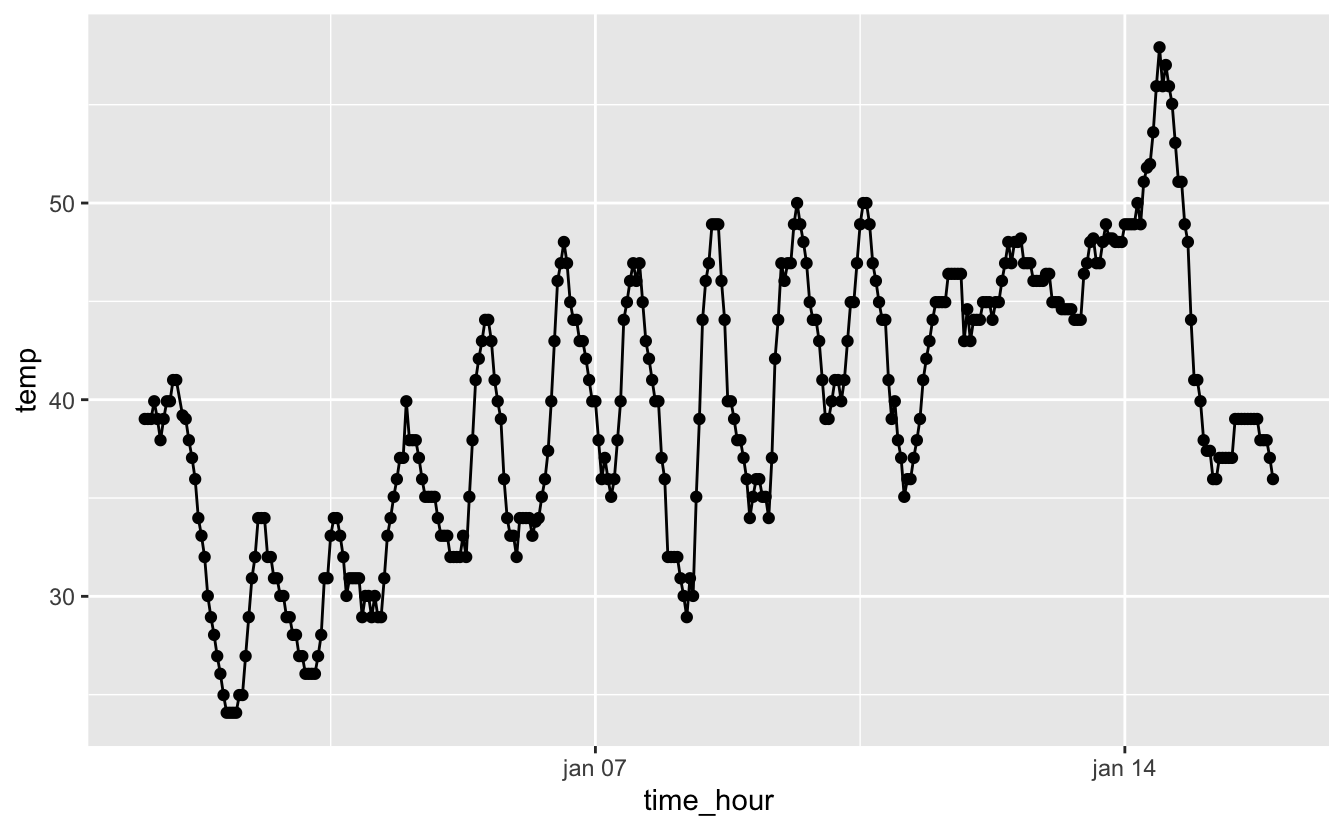
\includegraphics[width=0.9\linewidth]{figure/lineplotgraph-1} 

}

\caption{Températures horaires à l'aéroport de Newark entre le 1er et le 15 janvier 2013}\label{fig:lineplotgraph}
\end{figure}

Enfin, comme pour les points, il est possible de spécifier plusieurs
caractéristiques esthétiques des lignes, soit en les associant à des
variables, au sein de la fonction \texttt{aes()}, soit en les utilisant
en guise de paramètres pour modifier l'aspect général. Les arguments les
plus classiques sont une fois de plus \texttt{color} (ou
\texttt{colour}) pour modifier la couleur des lignes, \texttt{linetype}
pour modifier le type de lignes (continues, pointillées, tirets, etc),
et \texttt{size} pour modifier l'épaisseur des lignes.

Reprenons le jeu de données complet \texttt{weather}, et filtrons
uniquement les dates comprises entre le premier et le 15 janvier, mais
cette fois pour les 3 aéroports de New York :

\begin{Shaded}
\begin{Highlighting}[]
\NormalTok{small_weather_airports <-}\StringTok{ }\NormalTok{weather }\OperatorTok\StringTok{ }
\StringTok{  }\KeywordTok{filter}\NormalTok{(month }\OperatorTok{==}\StringTok{ }\DecValTok{1}\NormalTok{,}
\NormalTok{         day }\OperatorTok{<=}\StringTok{ }\DecValTok{15}\NormalTok{)}
\end{Highlighting}
\end{Shaded}

Nous pouvons maintenant réaliser un ``linegraph'' sur lequel une courbe
apparaîtra pour chaque aéroport. Pour cela, nous devons associer la
variable \texttt{origin} à un attribut esthétique des lignes. Par
exemple :

\begin{Shaded}
\begin{Highlighting}[]
\KeywordTok{ggplot}\NormalTok{(}\DataTypeTok{data =}\NormalTok{ small_weather_airports, }\DataTypeTok{mapping =} \KeywordTok{aes}\NormalTok{(}\DataTypeTok{x =}\NormalTok{ time_hour, }\DataTypeTok{y =}\NormalTok{ temp)) }\OperatorTok{+}
\StringTok{  }\KeywordTok{geom_line}\NormalTok{(}\KeywordTok{aes}\NormalTok{(}\DataTypeTok{color =}\NormalTok{ origin))}
\end{Highlighting}
\end{Shaded}

\begin{figure}[htpb]

{\centering 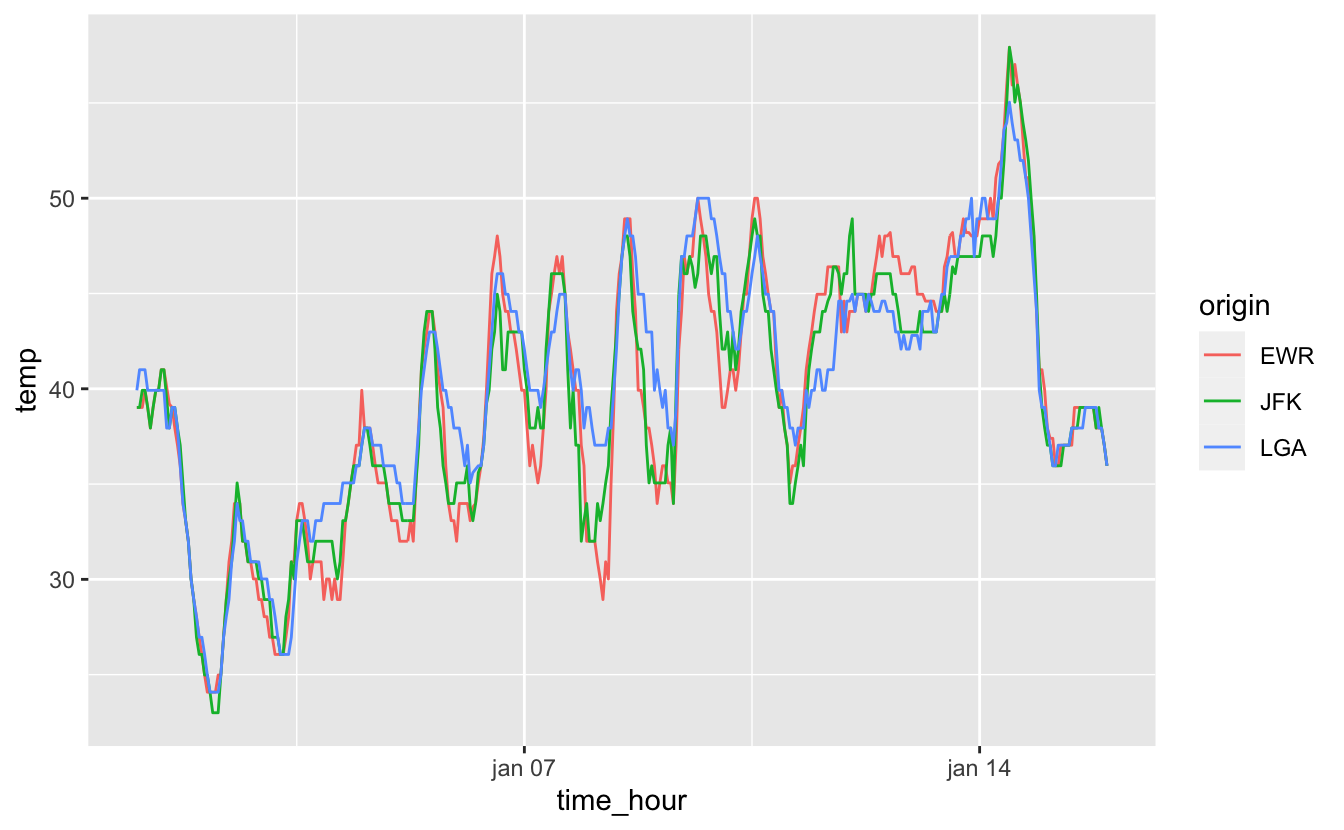
\includegraphics[width=0.9\linewidth]{figure/linecolor-1} 

}

\caption{Températures horaires des 3 aéroports de New York entre le 1er et le 15 janvier 2013}\label{fig:linecolor}
\end{figure}

Ou bien :

\begin{Shaded}
\begin{Highlighting}[]
\KeywordTok{ggplot}\NormalTok{(}\DataTypeTok{data =}\NormalTok{ small_weather_airports, }\DataTypeTok{mapping =} \KeywordTok{aes}\NormalTok{(}\DataTypeTok{x =}\NormalTok{ time_hour, }\DataTypeTok{y =}\NormalTok{ temp)) }\OperatorTok{+}
\StringTok{  }\KeywordTok{geom_line}\NormalTok{(}\KeywordTok{aes}\NormalTok{(}\DataTypeTok{linetype =}\NormalTok{ origin))}
\end{Highlighting}
\end{Shaded}

\begin{figure}[htpb]

{\centering 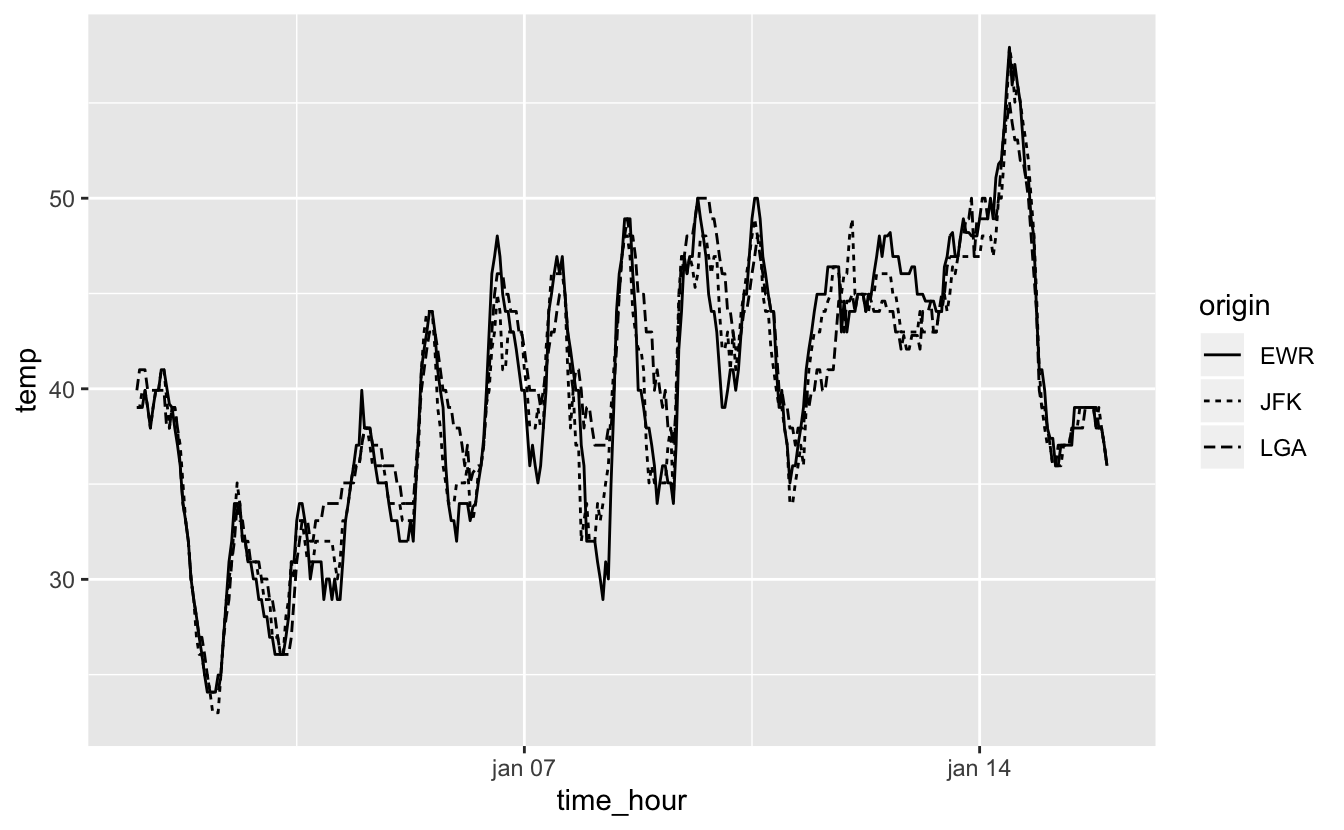
\includegraphics[width=0.9\linewidth]{figure/linetype-1} 

}

\caption{Températures horaires des 3 aéroports de New York entre le 1er et le 15 janvier 2013}\label{fig:linetype}
\end{figure}

Ou encore :

\begin{Shaded}
\begin{Highlighting}[]
\KeywordTok{ggplot}\NormalTok{(}\DataTypeTok{data =}\NormalTok{ small_weather_airports, }\DataTypeTok{mapping =} \KeywordTok{aes}\NormalTok{(}\DataTypeTok{x =}\NormalTok{ time_hour, }\DataTypeTok{y =}\NormalTok{ temp)) }\OperatorTok{+}
\StringTok{  }\KeywordTok{geom_line}\NormalTok{(}\KeywordTok{aes}\NormalTok{(}\DataTypeTok{color =}\NormalTok{ origin, }\DataTypeTok{linetype =}\NormalTok{ origin))}
\end{Highlighting}
\end{Shaded}

\begin{figure}[htpb]

{\centering 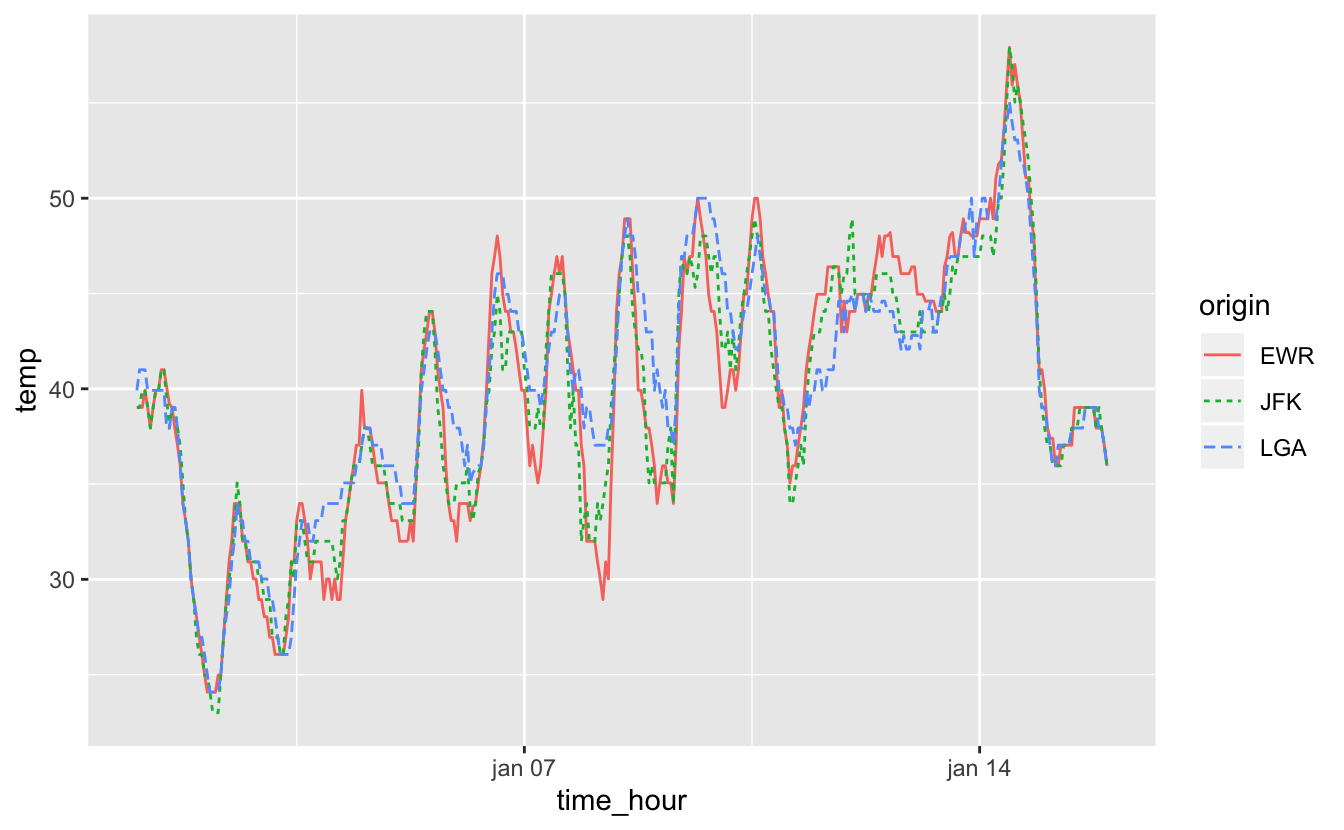
\includegraphics[width=0.9\linewidth]{figure/linetypecolor-1} 

}

\caption{Températures horaires des 3 aéroports de New York entre le 1er et le 15 janvier 2013}\label{fig:linetypecolor}
\end{figure}

\hypertarget{a-quel-endroit-placer-aes-et-les-arguments-color-size-etc.}{%
\subsubsection{\texorpdfstring{À quel endroit placer \texttt{aes()} et
les arguments \texttt{color}, \texttt{size}, etc.
?}{À quel endroit placer aes() et les arguments color, size, etc. ?}}\label{a-quel-endroit-placer-aes-et-les-arguments-color-size-etc.}}

Jusqu'à maintenant, pour spécifier les associations entre certaines
variables et les caractéristiques esthétiques d'un graphique, nous avons
été amenés à utiliser la fonction \texttt{aes()} à 2 endroits distincts
:

\begin{enumerate}
\def\labelenumi{\arabic{enumi}.}
\tightlist
\item
  au sein de la fonction \texttt{ggplot()}
\item
  au sein des fonctions \texttt{geom\_XXX()}
\end{enumerate}

Comment choisir l'endroit où renseigner \texttt{aes()} ? Pour bien
comprendre, reprenons l'exemple du graphique \ref{fig:lineplotgraph} sur
lequel nous avions ajouté 2 couches contenant chacune un objet
géométrique différent (afin de gagner de la place, j'omets
volontairement le nom des arguments \texttt{data} et \texttt{mapping}
dans la fonction \texttt{ggplot()}) :

\begin{Shaded}
\begin{Highlighting}[]
\KeywordTok{ggplot}\NormalTok{(small_weather, }\KeywordTok{aes}\NormalTok{(}\DataTypeTok{x =}\NormalTok{ time_hour, }\DataTypeTok{y =}\NormalTok{ temp)) }\OperatorTok{+}
\StringTok{  }\KeywordTok{geom_line}\NormalTok{() }\OperatorTok{+}
\StringTok{  }\KeywordTok{geom_point}\NormalTok{()}
\end{Highlighting}
\end{Shaded}

\begin{figure}[htpb]

{\centering 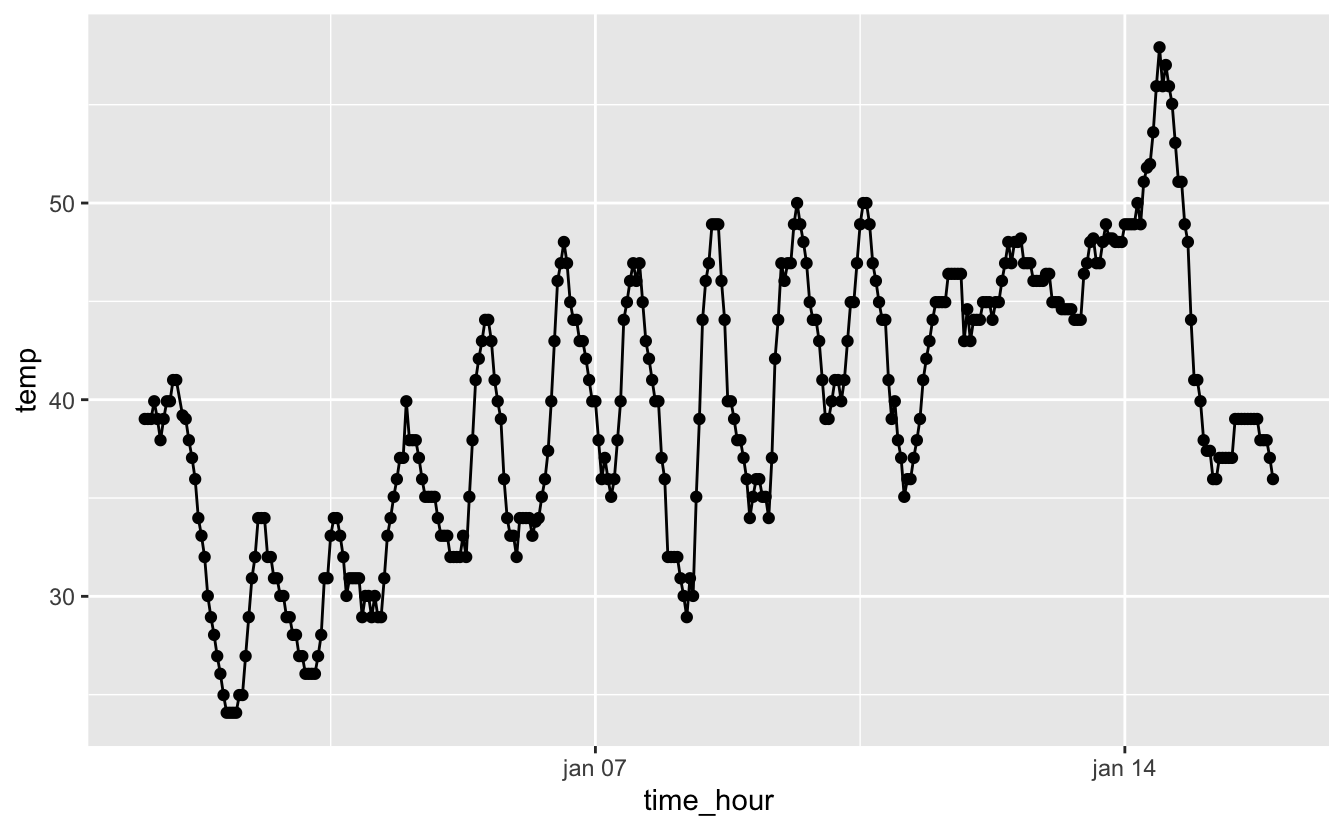
\includegraphics[width=0.9\linewidth]{figure/lineplotgraph2-1} 

}

\caption{Températures horaires à l'aéroport de Newark entre le 1er et le 15 janvier 2013}\label{fig:lineplotgraph2}
\end{figure}

Voyons ce qui se passe si on associe la variable \texttt{wind\_speed} à
l'esthétique \texttt{color}, à plusieurs endroits du code ci-dessus.
Comparez les trois syntaxes et observez les différences entre les 3
graphiques obtenus :

\begin{Shaded}
\begin{Highlighting}[]
\KeywordTok{ggplot}\NormalTok{(small_weather, }\KeywordTok{aes}\NormalTok{(}\DataTypeTok{x =}\NormalTok{ time_hour, }\DataTypeTok{y =}\NormalTok{ temp, }\DataTypeTok{color =}\NormalTok{ wind_speed)) }\OperatorTok{+}
\StringTok{  }\KeywordTok{geom_line}\NormalTok{() }\OperatorTok{+}
\StringTok{  }\KeywordTok{geom_point}\NormalTok{()}
\end{Highlighting}
\end{Shaded}

\begin{figure}[htpb]

{\centering 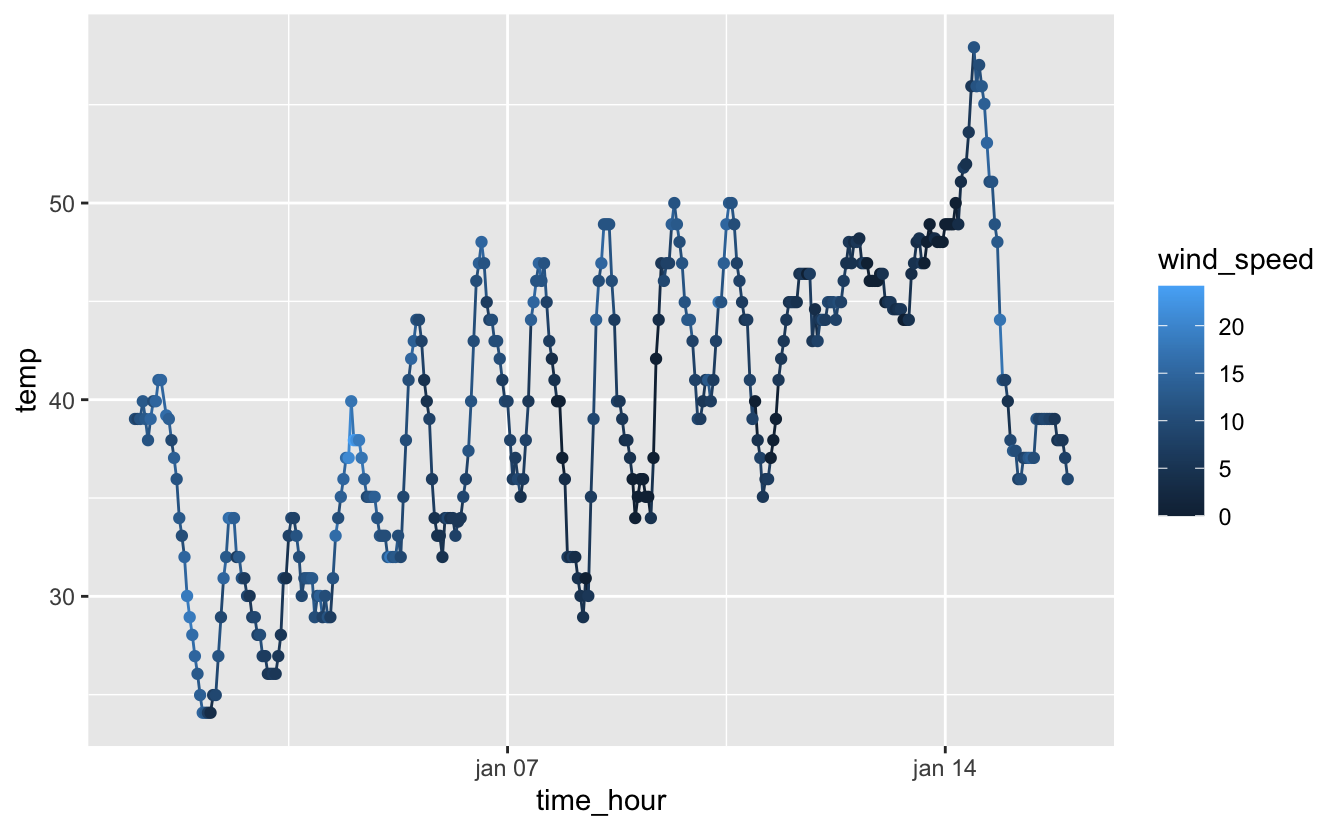
\includegraphics[width=0.9\linewidth]{figure/wind-1} 

}

\caption{Températures horaires et vitesse du vent à l'aéroport de Newark entre le 1er et le 15 janvier 2013}\label{fig:wind}
\end{figure}

\begin{Shaded}
\begin{Highlighting}[]
\KeywordTok{ggplot}\NormalTok{(small_weather, }\KeywordTok{aes}\NormalTok{(}\DataTypeTok{x =}\NormalTok{ time_hour, }\DataTypeTok{y =}\NormalTok{ temp)) }\OperatorTok{+}
\StringTok{  }\KeywordTok{geom_line}\NormalTok{(}\KeywordTok{aes}\NormalTok{(}\DataTypeTok{color =}\NormalTok{ wind_speed)) }\OperatorTok{+}
\StringTok{  }\KeywordTok{geom_point}\NormalTok{()}
\end{Highlighting}
\end{Shaded}

\begin{figure}[htpb]

{\centering 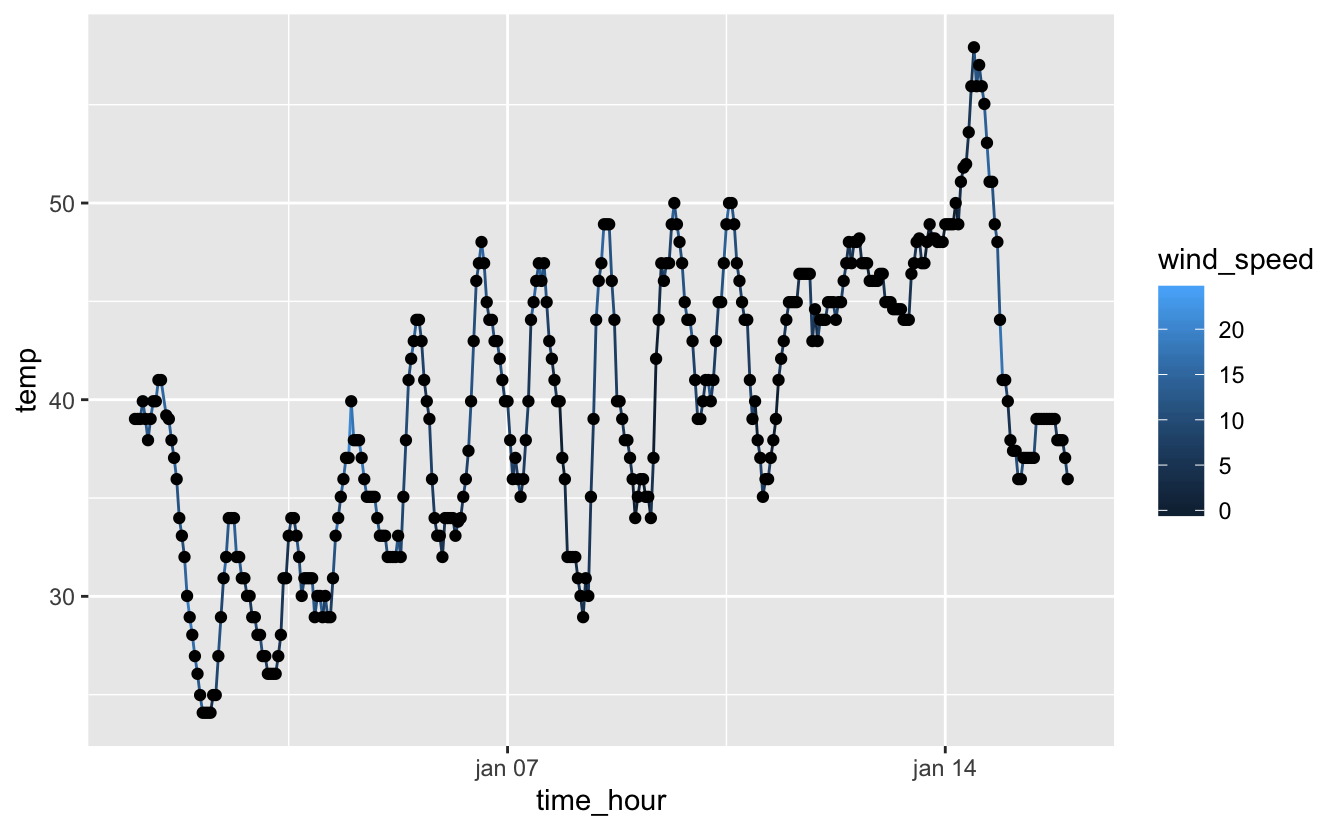
\includegraphics[width=0.9\linewidth]{figure/wind2-1} 

}

\caption{Températures horaires et vitesse du vent à l'aéroport de Newark entre le 1er et le 15 janvier 2013}\label{fig:wind2}
\end{figure}

\begin{Shaded}
\begin{Highlighting}[]
\KeywordTok{ggplot}\NormalTok{(small_weather, }\KeywordTok{aes}\NormalTok{(}\DataTypeTok{x =}\NormalTok{ time_hour, }\DataTypeTok{y =}\NormalTok{ temp)) }\OperatorTok{+}
\StringTok{  }\KeywordTok{geom_line}\NormalTok{() }\OperatorTok{+}
\StringTok{  }\KeywordTok{geom_point}\NormalTok{(}\KeywordTok{aes}\NormalTok{(}\DataTypeTok{color =}\NormalTok{ wind_speed))}
\end{Highlighting}
\end{Shaded}

\begin{figure}[htpb]

{\centering 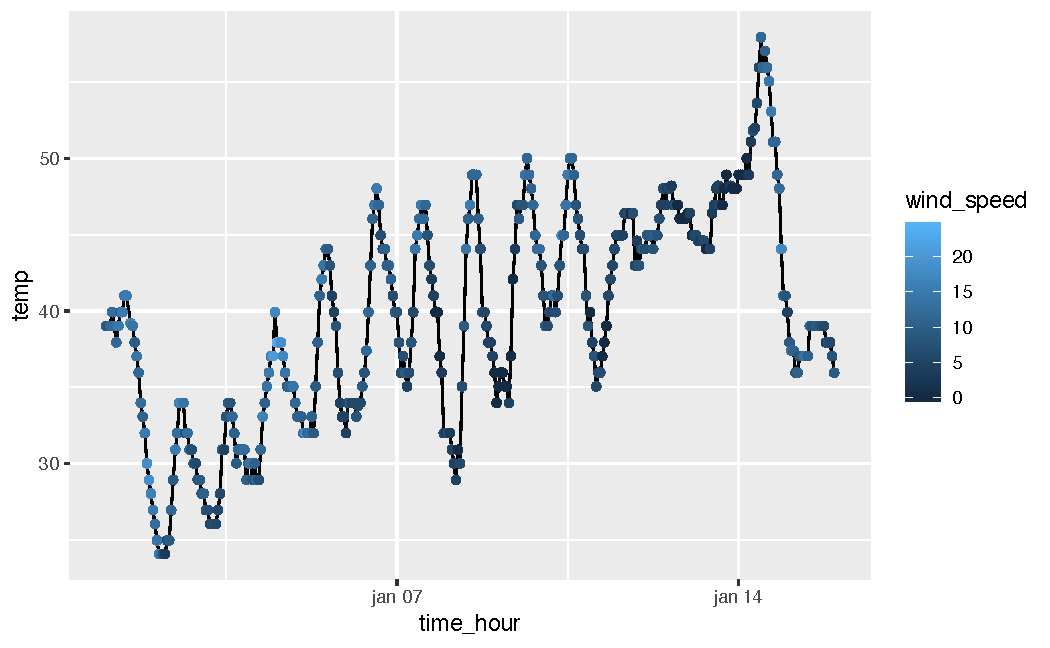
\includegraphics[width=0.9\linewidth]{figure/wind3-1} 

}

\caption{Températures horaires et vitesse du vent à l'aéroport de Newark entre le 1er et le 15 janvier 2013}\label{fig:wind3}
\end{figure}

Vous l'aurez compris, lorsque l'on spécifie \texttt{aes()} à l'intérieur
de la fonction \texttt{ggplot()}, les associations de variables et
d'esthétiques sont appliquées à tous les objets géométriques, donc à
toutes les autres couches. En revanche, quand \texttt{aes()} est
spécifié dans une couche donnée, les réglages ne s'appliquent qu'à cette
couche spécifique.

En l'occurence, si le même réglage est spécifié dans la fonction
\texttt{ggplot()} et dans une fonction \texttt{geom\_XXX()}, c'est le
réglage spécifié dans l'objet géométrique qui l'emporte :

\begin{Shaded}
\begin{Highlighting}[]
\KeywordTok{ggplot}\NormalTok{(small_weather, }\KeywordTok{aes}\NormalTok{(}\DataTypeTok{x =}\NormalTok{ time_hour, }\DataTypeTok{y =}\NormalTok{ temp, }\DataTypeTok{color =}\NormalTok{ wind_speed)) }\OperatorTok{+}
\StringTok{  }\KeywordTok{geom_line}\NormalTok{(}\DataTypeTok{color =} \StringTok{"orange"}\NormalTok{) }\OperatorTok{+}
\StringTok{  }\KeywordTok{geom_point}\NormalTok{()}
\end{Highlighting}
\end{Shaded}

\begin{figure}[htpb]

{\centering 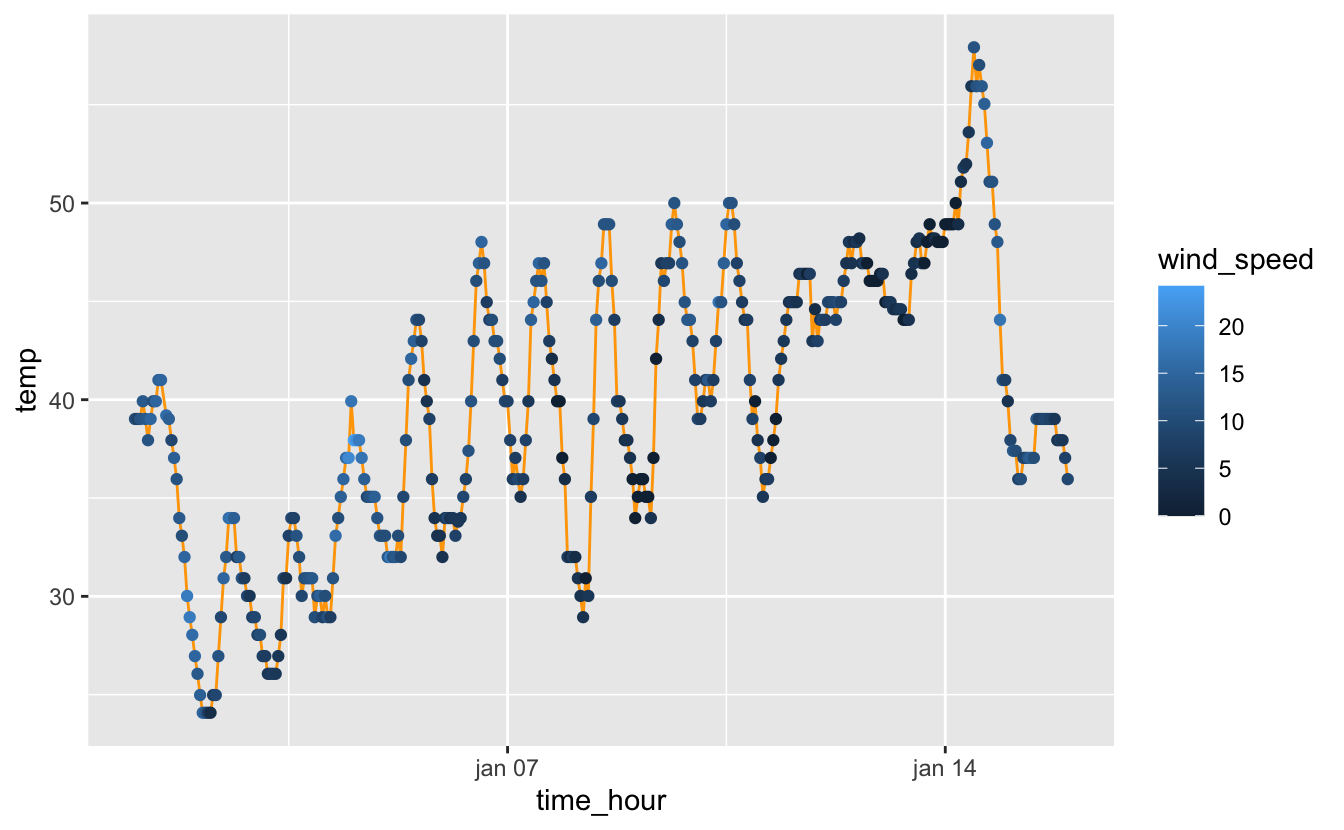
\includegraphics[width=0.9\linewidth]{figure/wind4-1} 

}

\caption{Températures horaires et vitesse du vent à l'aéroport de Newark entre le 1er et le 15 janvier 2013}\label{fig:wind4}
\end{figure}

il est ainsi possible de spécifier des éléments esthétiques qui
s'appliqueront à toutes les couches d'un graphique, et d'autres qui ne
s'appliqueront qu'à une couche spécifique, qu'à un objet géométrique
particulier.

\begin{center}\rule{0.5\linewidth}{\linethickness}\end{center}

\hypertarget{histogram}{%
\subsection{Les histogrammes}\label{histogram}}

Un histogramme permet de visualiser la distribution \textbf{d'une
variable} numérique continue. Contrairement aux deux types de graphiques
vus précédemment, il sera donc inutile de préciser la variable à
associer à l'axe des ordonnées : R la calcule automatiquement pour nous
lorsque nous faisons appel à la fonction \texttt{geom\_histogram()} pour
créer un objet géométrique ``histogramme''.

\hypertarget{lobjet-geom_histogram}{%
\subsubsection{\texorpdfstring{L'objet
\texttt{geom\_histogram()}}{L'objet geom\_histogram()}}\label{lobjet-geom_histogram}}

Si on reprend le jeu de données \texttt{weather}, on peut par exemple
s'intéresser à la distribution des températures tout au long de l'année
:

\begin{Shaded}
\begin{Highlighting}[]
\KeywordTok{ggplot}\NormalTok{(weather, }\KeywordTok{aes}\NormalTok{(}\DataTypeTok{x =}\NormalTok{ temp)) }\OperatorTok{+}
\StringTok{  }\KeywordTok{geom_histogram}\NormalTok{()}
\end{Highlighting}
\end{Shaded}

\begin{verbatim}
`stat_bin()` using `bins = 30`. Pick better value with `binwidth`.
\end{verbatim}

\begin{figure}[htpb]

{\centering 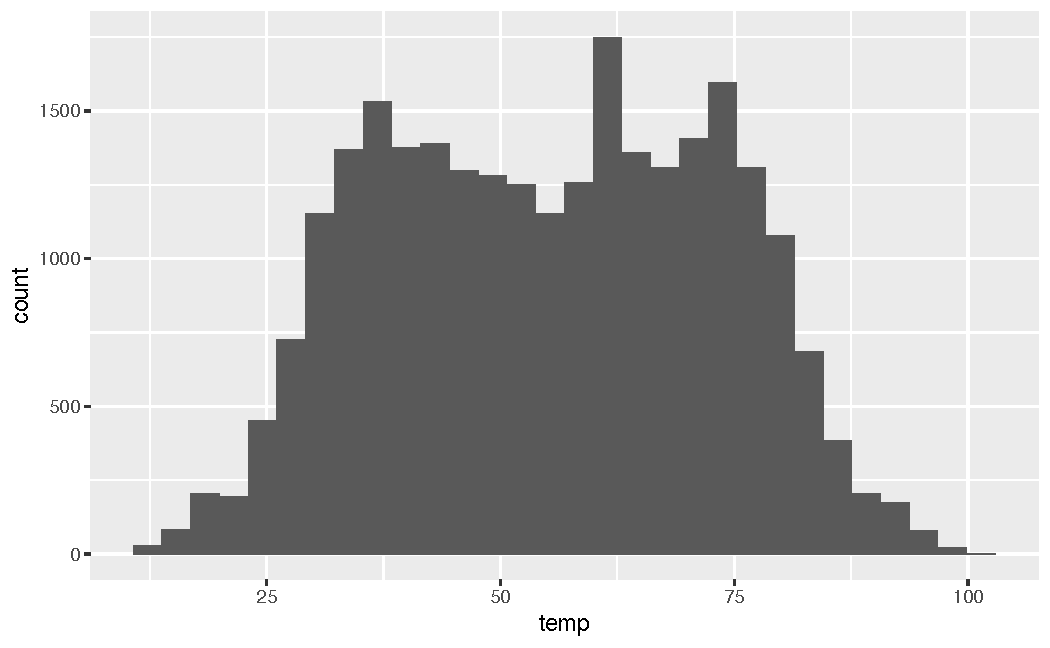
\includegraphics[width=0.9\linewidth]{figure/unnamed-chunk-46-1} 

}

\caption{Histogramme des températures enregistrées en 2013 dans les 3 aéroports de New York}\label{fig:unnamed-chunk-46}
\end{figure}

On observe plusieurs choses :

\begin{enumerate}
\def\labelenumi{\arabic{enumi}.}
\tightlist
\item
  La distribution semble globalement bimodale avec un pic autour de
  36-37 degrés farenheit (2 à 3 ºC) et un autre autour de 65-70 degrés
  farenheit (18-21 ºC).
\item
  Les températures ont varié de 12 degrés farenheit (-11ºC) à 100 degrés
  farenheit (près de 38ºC).
\item
  R nous avertit qu'une valeur non finie n'a pas pu être intégrée
\item
  R nou indique qu'il a choisi de représenter 30 classes de températures
  (\texttt{bins\ =\ 30}). C'est la valeur par défaut. R nous conseille
  de choisir une valeur plus appropriée.
\end{enumerate}

Comme pour les nuages de points utilisant les symboles 21 à 24, il est
possible de spécifier la couleur de remplissage des barres avec
l'argument \texttt{fill} et la couleur du contour des barres avec
l'argument \texttt{color} :

\begin{Shaded}
\begin{Highlighting}[]
\KeywordTok{ggplot}\NormalTok{(weather, }\KeywordTok{aes}\NormalTok{(}\DataTypeTok{x =}\NormalTok{ temp)) }\OperatorTok{+}
\StringTok{  }\KeywordTok{geom_histogram}\NormalTok{(}\DataTypeTok{fill =} \StringTok{"steelblue"}\NormalTok{, }\DataTypeTok{color =} \StringTok{"grey80"}\NormalTok{)}
\end{Highlighting}
\end{Shaded}

\begin{figure}[htpb]

{\centering 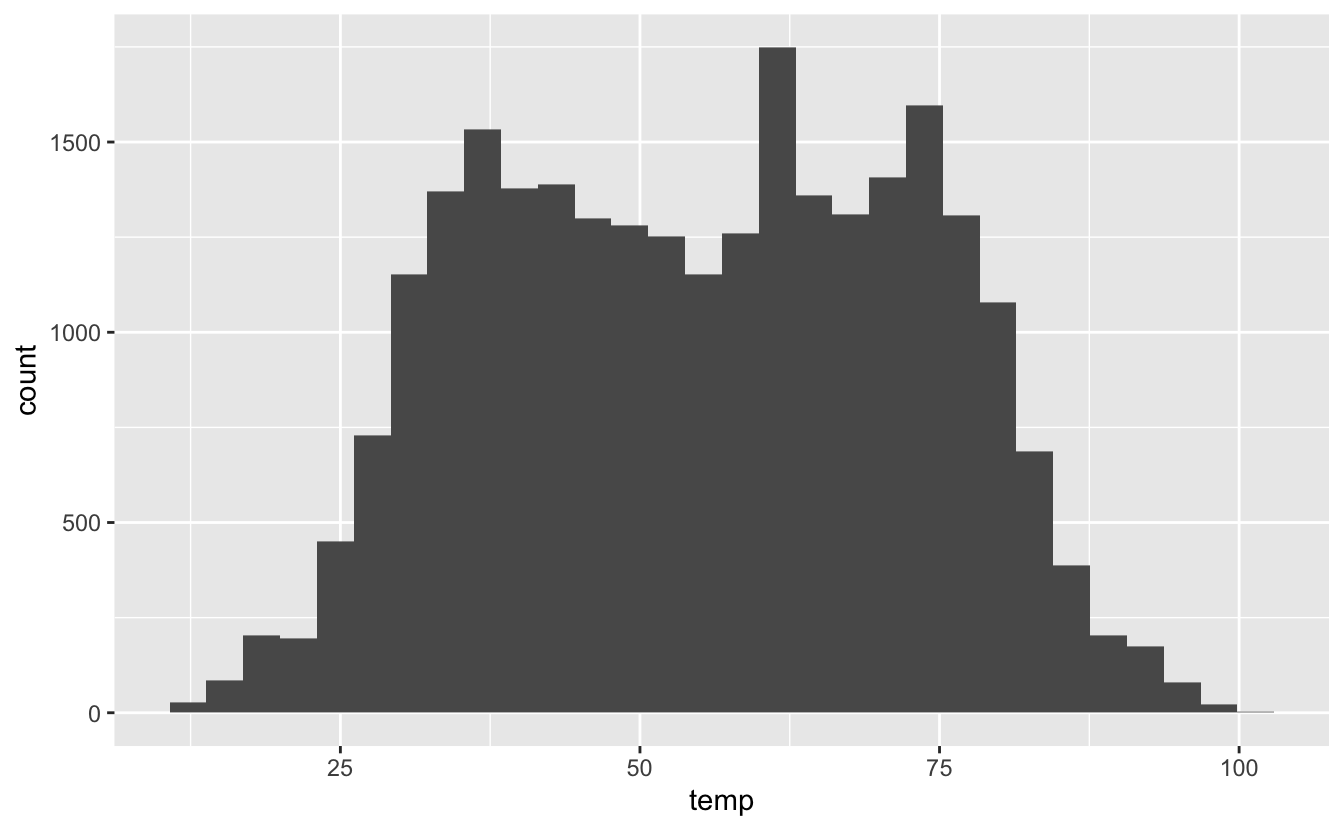
\includegraphics[width=0.9\linewidth]{figure/unnamed-chunk-47-1} 

}

\caption{Utilisation des arguments `fill` et `color` pour modifier l'aspect de l'histogramme.}\label{fig:unnamed-chunk-47}
\end{figure}

\hypertarget{la-taille-des-classes}{%
\subsubsection{La taille des classes}\label{la-taille-des-classes}}

Par défaut, R choisit arbitrairement de représenter 30 classes. Ce n'est
que rarement le bon choix, et il est souvent nécessaire de tâtonner pour
trouver le nombre de classes : celui qui permet d'avoir une idée
correcte de la distribution des données.

Il est possible d'ajuster les caractéristiques des classes de
l'histogramme de l'une des 3 façons suivantes :

\begin{enumerate}
\def\labelenumi{\arabic{enumi}.}
\tightlist
\item
  en ajustant le nombre de classes avec \texttt{bins}
\item
  en précisant la largeur des classes avec \texttt{binwidth}
\item
  en fournissant manuellement les limites des classes avec
  \texttt{breaks}
\end{enumerate}

\begin{Shaded}
\begin{Highlighting}[]
\KeywordTok{ggplot}\NormalTok{(weather, }\KeywordTok{aes}\NormalTok{(}\DataTypeTok{x =}\NormalTok{ temp)) }\OperatorTok{+}
\StringTok{  }\KeywordTok{geom_histogram}\NormalTok{(}\DataTypeTok{bins =} \DecValTok{60}\NormalTok{, }\DataTypeTok{color =} \StringTok{"white"}\NormalTok{)}
\end{Highlighting}
\end{Shaded}

\begin{figure}[htpb]

{\centering 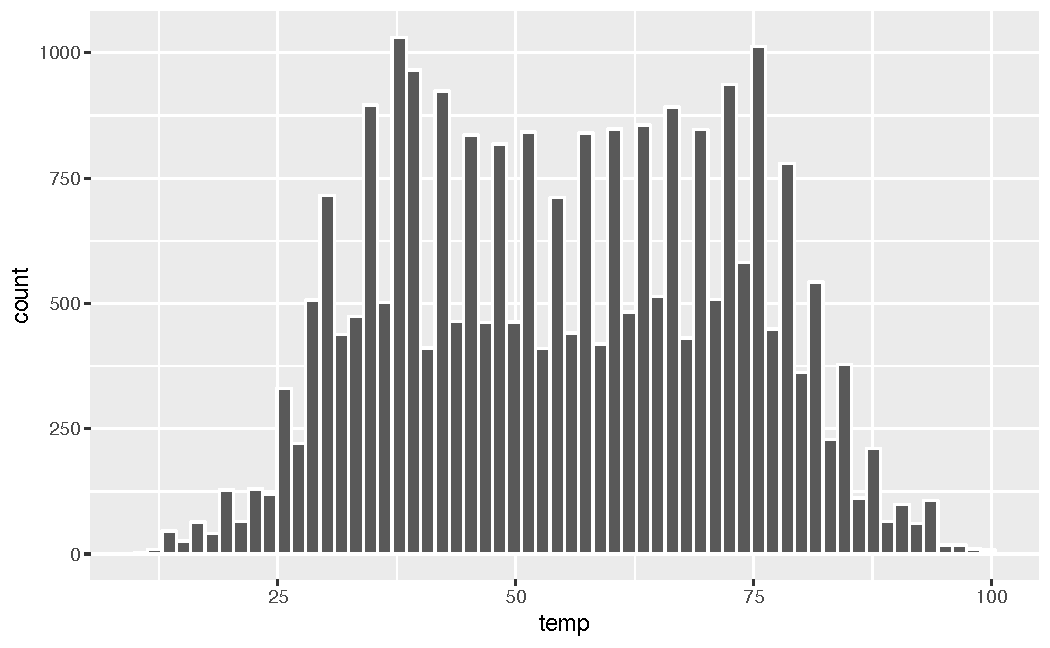
\includegraphics[width=0.9\linewidth]{figure/unnamed-chunk-48-1} 

}

\caption{Modification du nombre de classes}\label{fig:unnamed-chunk-48}
\end{figure}

Ici, augmenter le nombre de classes à 60 permet de prendre conscience
que la distribution n'est pas aussi lisse qu'elle en avait l'air.
L'ajout d'une couche supplémentaire avec la fonction
\texttt{geom\_rug()} (``a rug'' est un tapis en français) permet de
prendre conscience que les données de température ne sont pas aussi
continues qu'on pouvait le croire :

\begin{Shaded}
\begin{Highlighting}[]
\KeywordTok{ggplot}\NormalTok{(weather, }\KeywordTok{aes}\NormalTok{(}\DataTypeTok{x =}\NormalTok{ temp)) }\OperatorTok{+}
\StringTok{  }\KeywordTok{geom_histogram}\NormalTok{(}\DataTypeTok{bins =} \DecValTok{60}\NormalTok{, }\DataTypeTok{color =} \StringTok{"white"}\NormalTok{) }\OperatorTok{+}
\StringTok{  }\KeywordTok{geom_rug}\NormalTok{(}\DataTypeTok{alpha =} \FloatTok{0.1}\NormalTok{)}
\end{Highlighting}
\end{Shaded}

\begin{figure}[htpb]

{\centering 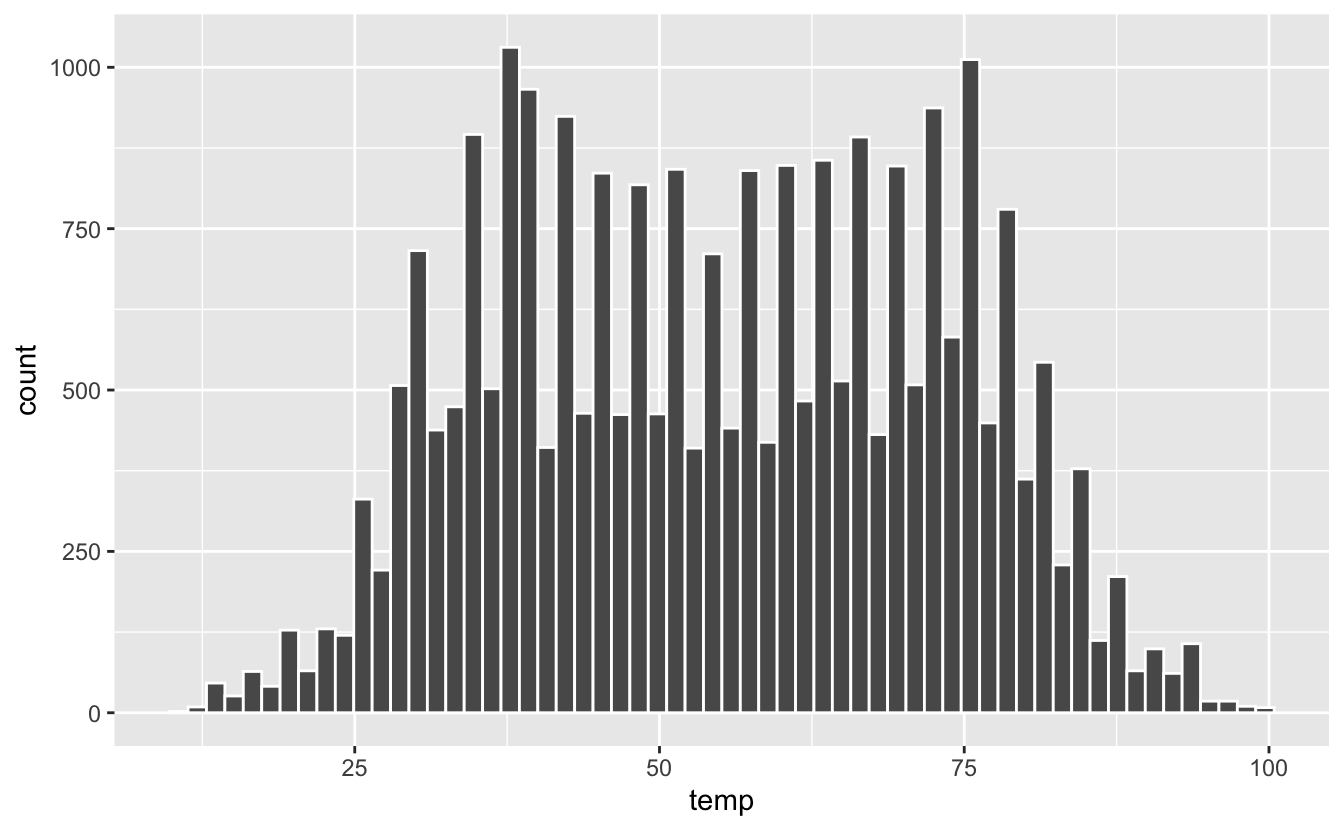
\includegraphics[width=0.9\linewidth]{figure/unnamed-chunk-49-1} 

}

\caption{Ajout des données brutes sous forme de 'tapis' (`rug`) sous l'histogramme.}\label{fig:unnamed-chunk-49}
\end{figure}

Notez la transparence importante utilisée pour \texttt{geom\_rug()}. On
constate que la précision des relevés de température n'est en fait que
de quelques dixièmes de degrés.

On peut également modifier la largeur des classes avec \texttt{binwidth}
:

\begin{Shaded}
\begin{Highlighting}[]
\KeywordTok{ggplot}\NormalTok{(weather, }\KeywordTok{aes}\NormalTok{(}\DataTypeTok{x =}\NormalTok{ temp)) }\OperatorTok{+}
\StringTok{  }\KeywordTok{geom_histogram}\NormalTok{(}\DataTypeTok{binwidth =} \DecValTok{10}\NormalTok{, }\DataTypeTok{color =} \StringTok{"white"}\NormalTok{)}
\end{Highlighting}
\end{Shaded}

\begin{figure}[htpb]

{\centering 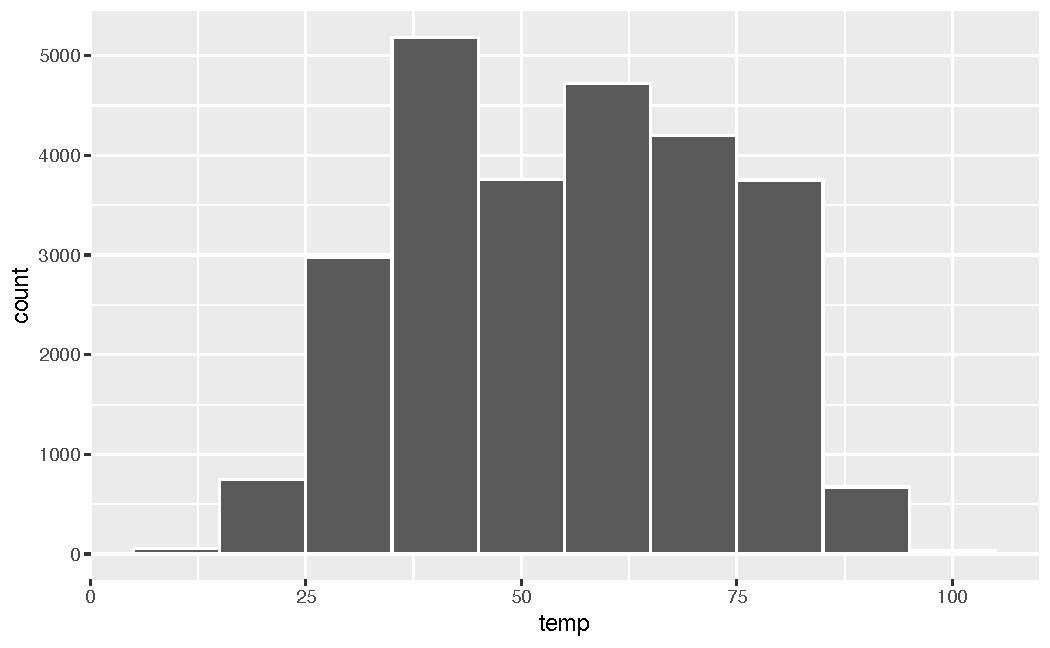
\includegraphics[width=0.9\linewidth]{figure/unnamed-chunk-50-1} 

}

\caption{Modification de la largeur des classes avec `binwidth`}\label{fig:unnamed-chunk-50}
\end{figure}

Ici chaque catégorie recouvre 10 degrés farenheit, ce qui est
probablement trop large puisque la bimodalité de la distribution est
devenue presque invisible. Enfin, il est possible de déterminer
manuellement les limites des classes souhaitées avec l'argument
\texttt{breaks} :

\begin{Shaded}
\begin{Highlighting}[]
\KeywordTok{ggplot}\NormalTok{(weather, }\KeywordTok{aes}\NormalTok{(}\DataTypeTok{x =}\NormalTok{ temp)) }\OperatorTok{+}
\StringTok{  }\KeywordTok{geom_histogram}\NormalTok{(}\DataTypeTok{breaks =} \KeywordTok{c}\NormalTok{(}\DecValTok{0}\NormalTok{, }\DecValTok{10}\NormalTok{, }\DecValTok{20}\NormalTok{, }\DecValTok{50}\NormalTok{, }\DecValTok{60}\NormalTok{, }\DecValTok{70}\NormalTok{, }\DecValTok{80}\NormalTok{, }\DecValTok{105}\NormalTok{), }\DataTypeTok{color =} \StringTok{"white"}\NormalTok{)}
\end{Highlighting}
\end{Shaded}

\begin{figure}[htpb]

{\centering 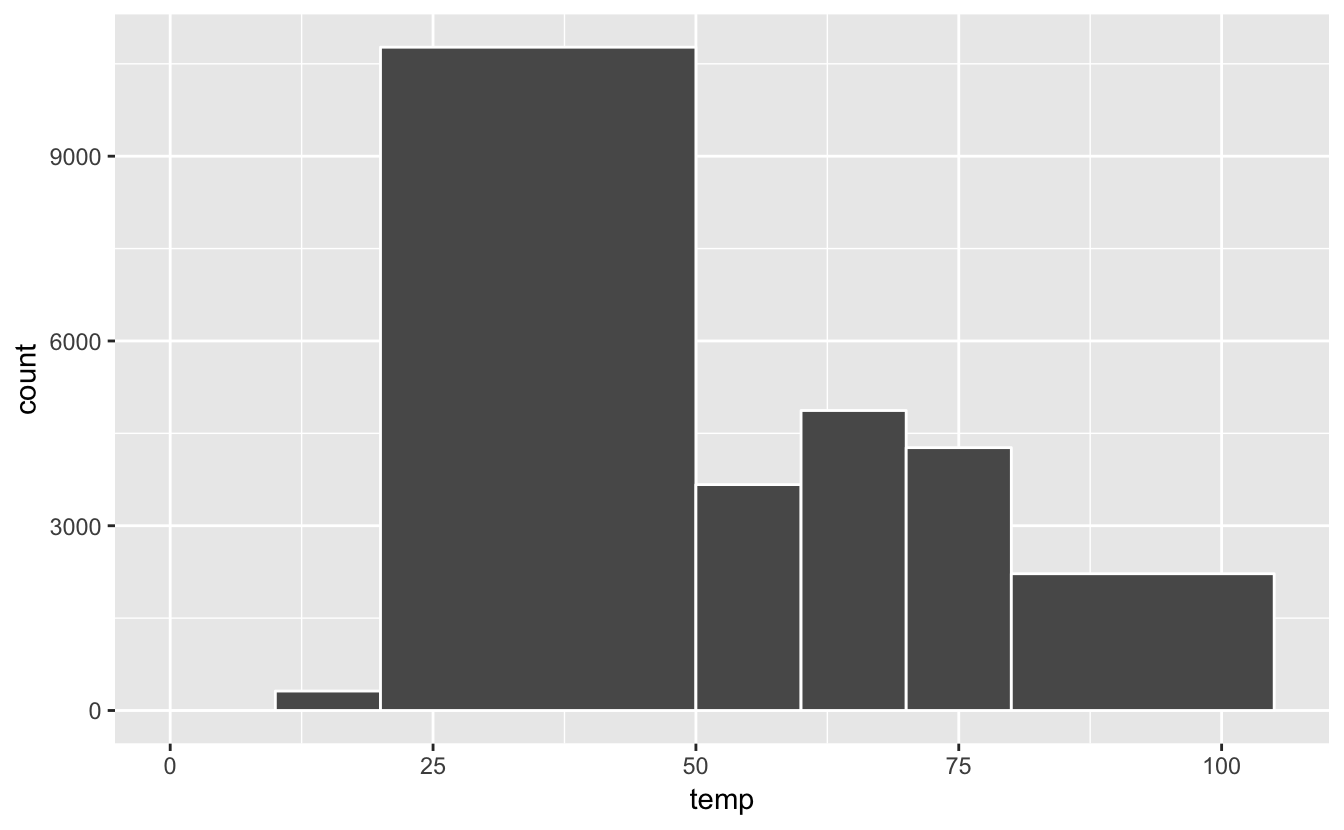
\includegraphics[width=0.9\linewidth]{figure/unnamed-chunk-51-1} 

}

\caption{Spécification manuelle des limites de classes de tailles (classes irrégulières)}\label{fig:unnamed-chunk-51}
\end{figure}

Vous constatez ici que les choix effectués ne sont pas très pertinents :
toutes les classes n'ont pas la même largeur. Cela rend l'interprétation
difficile. Il est donc vivement conseillé, pour spécifier
\texttt{breaks}, de créer des suites régulières, comme avec la fonction
\texttt{seq()} par exemple (consultez son fichier d'aide et les exemples
!) :

\begin{Shaded}
\begin{Highlighting}[]
\NormalTok{limits <-}\StringTok{ }\KeywordTok{seq}\NormalTok{(}\DataTypeTok{from =} \DecValTok{10}\NormalTok{, }\DataTypeTok{to =} \DecValTok{105}\NormalTok{, }\DataTypeTok{by =} \DecValTok{5}\NormalTok{)}
\NormalTok{limits}
\end{Highlighting}
\end{Shaded}

\begin{verbatim}
 [1]  10  15  20  25  30  35  40  45  50  55  60  65  70  75  80  85  90  95 100
[20] 105
\end{verbatim}

\begin{Shaded}
\begin{Highlighting}[]
\KeywordTok{ggplot}\NormalTok{(weather, }\KeywordTok{aes}\NormalTok{(}\DataTypeTok{x =}\NormalTok{ temp)) }\OperatorTok{+}
\StringTok{  }\KeywordTok{geom_histogram}\NormalTok{(}\DataTypeTok{breaks =}\NormalTok{ limits, }\DataTypeTok{color =} \StringTok{"white"}\NormalTok{)}
\end{Highlighting}
\end{Shaded}

\begin{figure}[htpb]

{\centering 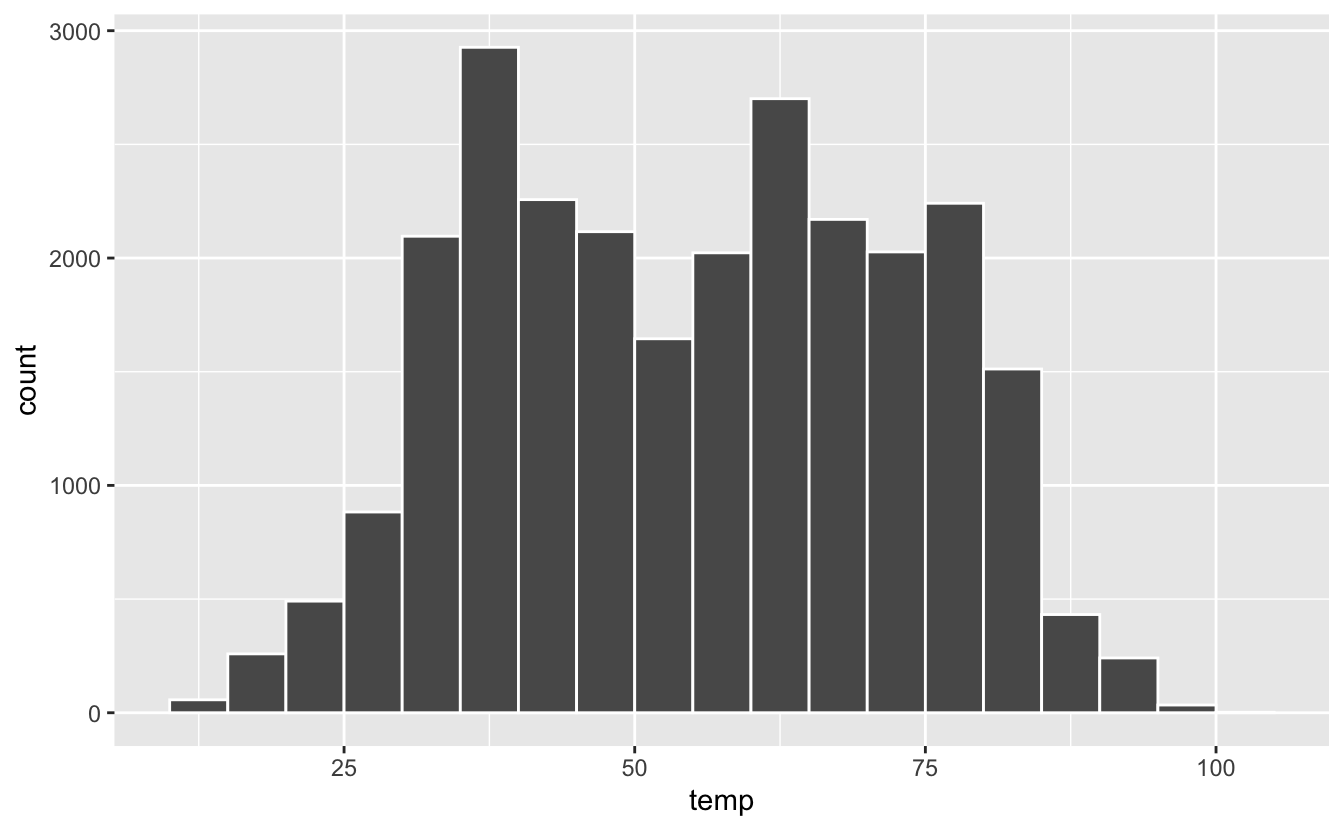
\includegraphics[width=0.9\linewidth]{figure/break-1} 

}

\caption{Un exemple d'utilisation de l'argument `break`}\label{fig:break}
\end{figure}

Il est important que toute la gamme des valeurs de \texttt{temp} soit
couverte par les limites des classes que nous avons définies, sinon,
certaines valeurs sont omises et l'histogramme est donc
incomplet/incorrect. Une façon de s'en assurer est d'afficher les résumé
des données pour la colonne \texttt{temp} du jeu de données
\texttt{weather} :

\begin{Shaded}
\begin{Highlighting}[]
\KeywordTok{summary}\NormalTok{(weather}\OperatorTok{$}\NormalTok{temp)}
\end{Highlighting}
\end{Shaded}

\begin{verbatim}
   Min. 1st Qu.  Median    Mean 3rd Qu.    Max.    NA's 
  10.94   39.92   55.40   55.26   69.98  100.04       1 
\end{verbatim}

On voit ici que les températures varien de 10.94 à 100.04 degrés
farenheit. Les classes que nous avons définies couvrent une plage de
température plus large (de 10 à 105). Toutes les données sont donc bien
intégrées à l'histogramme.

\begin{center}\rule{0.5\linewidth}{\linethickness}\end{center}

\hypertarget{facets}{%
\subsection{\texorpdfstring{Les
\texttt{facet}s}{Les facets}}\label{facets}}

\hypertarget{facet_wrap}{%
\subsubsection{\texorpdfstring{\texttt{facet\_wrap()}}{facet\_wrap()}}\label{facet_wrap}}

Nous l'avons indiqué plus haut, les \texttt{facet}s permettent de
scinder le jeux de données en plusieurs sous-groupes et de faire un
graphique pour chacun des sous-groupes.

Ainsi, si l'on souhaite connaître la distribution des températures pour
chaque mois de l'année 2013, plutôt que de faire ceci :

\begin{Shaded}
\begin{Highlighting}[]
\KeywordTok{ggplot}\NormalTok{(weather, }\KeywordTok{aes}\NormalTok{(}\DataTypeTok{x =}\NormalTok{ temp, }\DataTypeTok{fill =} \KeywordTok{factor}\NormalTok{(month))) }\OperatorTok{+}
\StringTok{  }\KeywordTok{geom_histogram}\NormalTok{(}\DataTypeTok{bins =} \DecValTok{20}\NormalTok{, }\DataTypeTok{color =} \StringTok{"grey30"}\NormalTok{)}
\end{Highlighting}
\end{Shaded}

\begin{figure}[htpb]

{\centering 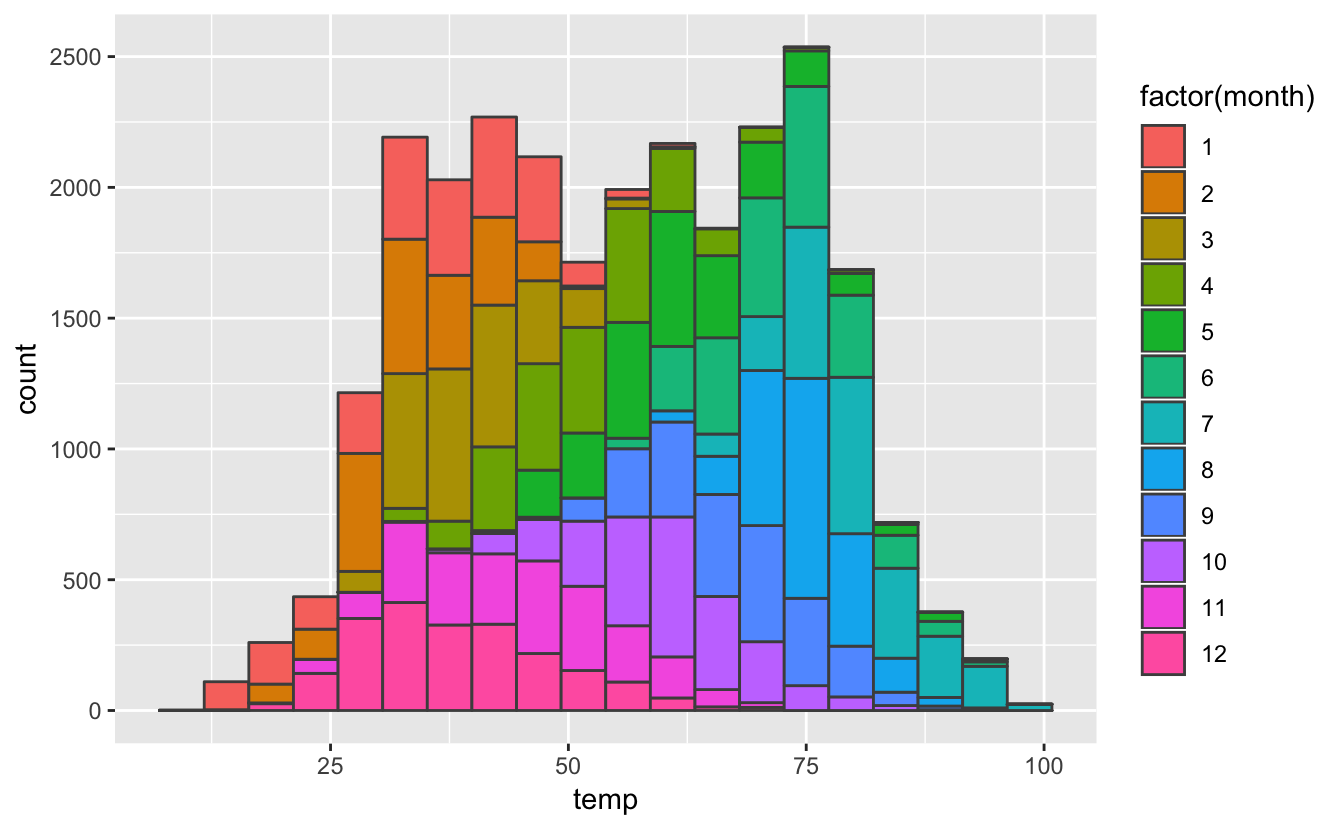
\includegraphics[width=0.9\linewidth]{figure/unnamed-chunk-53-1} 

}

\caption{Distribution des températures avec visualisation des données mensuelles.}\label{fig:unnamed-chunk-53}
\end{figure}

qui produit un graphique certes assez joli, mais difficile à
interpréter, mieux vaut faire ceci :

\begin{Shaded}
\begin{Highlighting}[]
\KeywordTok{ggplot}\NormalTok{(weather, }\KeywordTok{aes}\NormalTok{(}\DataTypeTok{x =}\NormalTok{ temp, }\DataTypeTok{fill =} \KeywordTok{factor}\NormalTok{(month))) }\OperatorTok{+}
\StringTok{  }\KeywordTok{geom_histogram}\NormalTok{(}\DataTypeTok{bins =} \DecValTok{20}\NormalTok{, }\DataTypeTok{color =} \StringTok{"grey30"}\NormalTok{) }\OperatorTok{+}
\StringTok{  }\KeywordTok{facet_wrap}\NormalTok{(}\OperatorTok{~}\KeywordTok{factor}\NormalTok{(month), }\DataTypeTok{ncol =} \DecValTok{3}\NormalTok{)}
\end{Highlighting}
\end{Shaded}

\textbackslash{}begin\{figure\}{[}htpb{]}

\{\centering 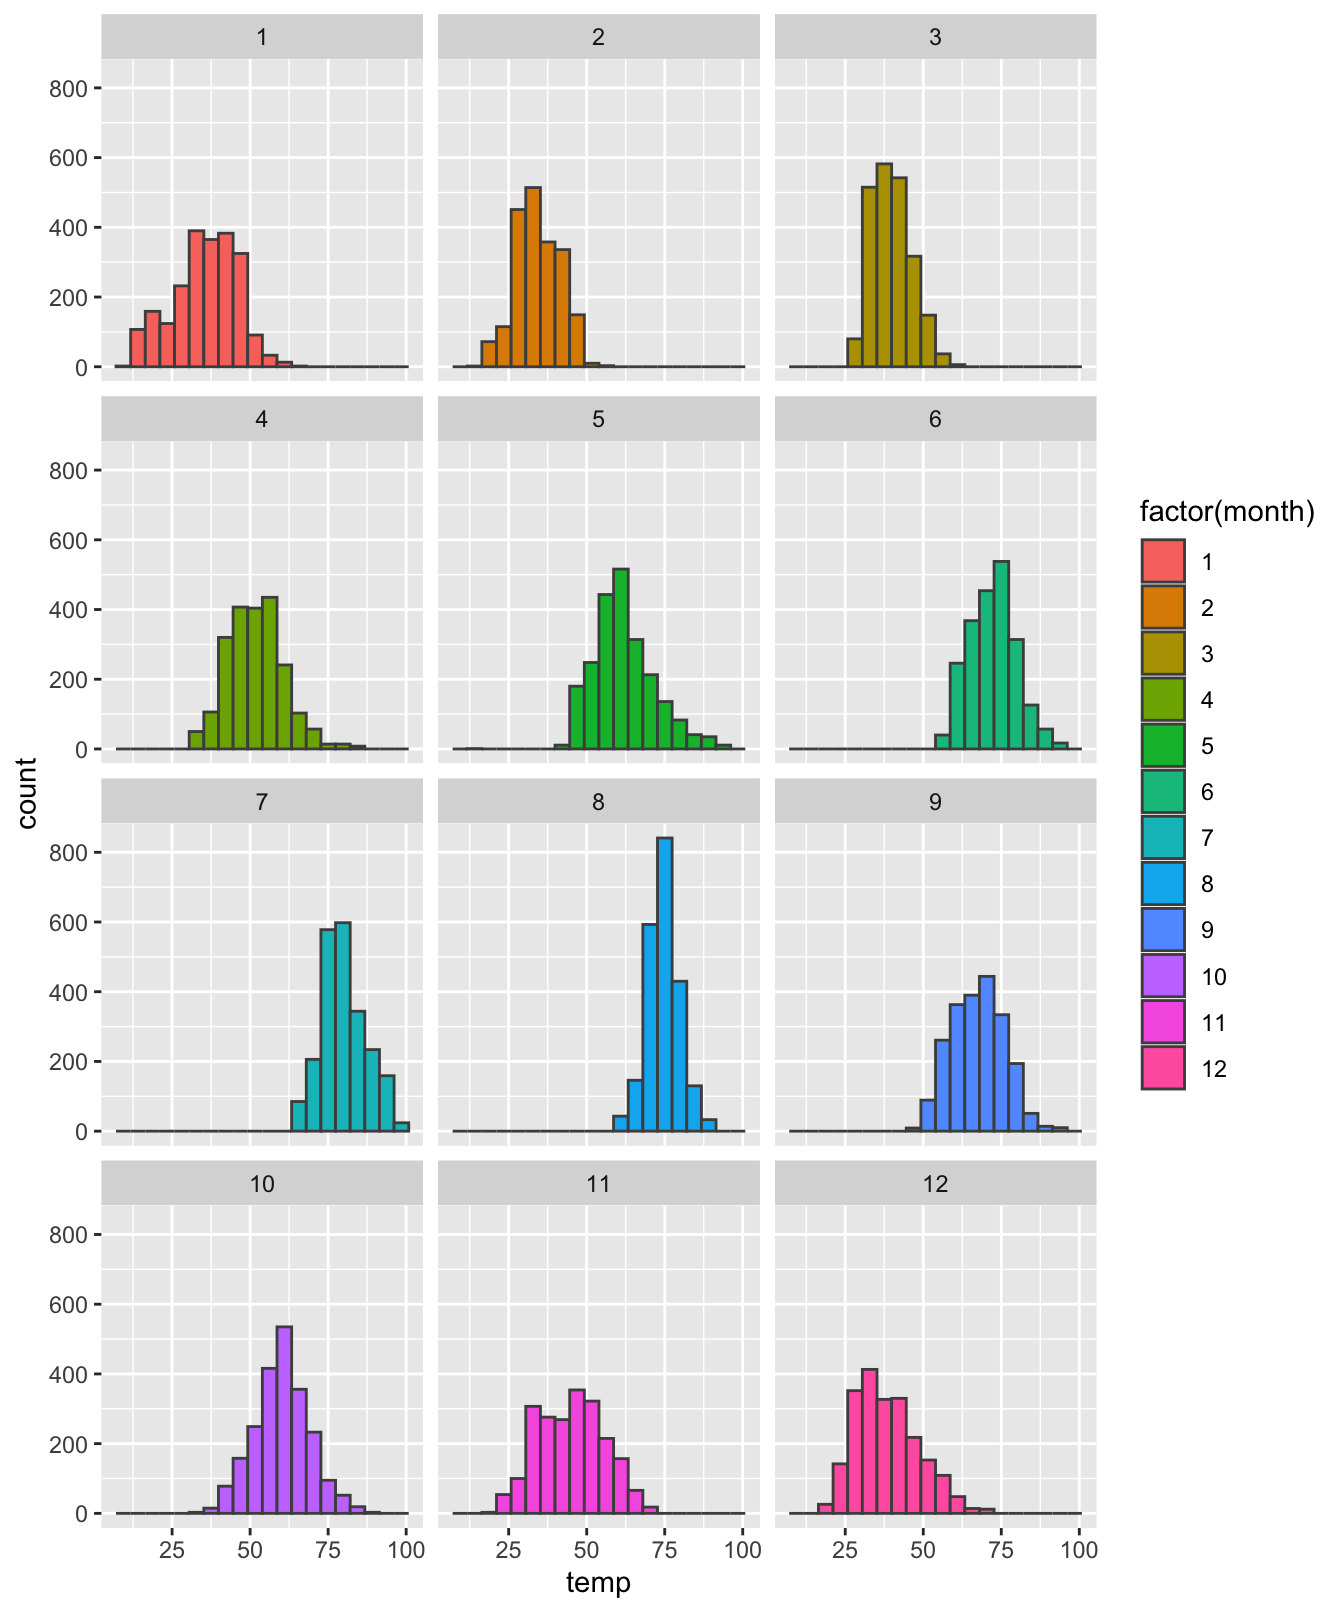
\includegraphics[width=0.9\linewidth]{figure/wrap-1}

\}

\textbackslash{}caption\{Un exemple d'utilisation de
\texttt{facet\_wrap()}\}\label{fig:wrap} \textbackslash{}end\{figure\}

La couche supplémentaire créée avec \texttt{facet\_wrap} permet donc de
scinder les données en fonction d'une variable. Attention à la syntaxe ;
il ne faut pas oublier le symbole \texttt{\textasciitilde{}} devant la
variable que l'on souhaite utiliser pour scinder les données. Il va sans
dire que la variable utilisée doit être catégorielle et non continue,
c'est la raison pour laquelle j'utilise la notation
\texttt{factor(month)} et non simplement \texttt{month}.

Avec la fonction \texttt{facet\_wrap()}, il est possible d'indiquer à R
comment les différents graphiques doivent être agencés en spécifiant
soit le nombre de colonnes souhaité avec \texttt{ncol}, soit le nombre
de lignes souhaitées avec \texttt{nrow}.

\hypertarget{facet_grid}{%
\subsubsection{\texorpdfstring{\texttt{facet\_grid()}}{facet\_grid()}}\label{facet_grid}}

Une autre fonction nommée \texttt{facet\_grid()} permet d'agencer des
sous-graphiques selon 2 variables catégorielles. Par exemple :

\begin{Shaded}
\begin{Highlighting}[]
\KeywordTok{ggplot}\NormalTok{(weather, }\KeywordTok{aes}\NormalTok{(}\DataTypeTok{x =}\NormalTok{ temp, }\DataTypeTok{fill =} \KeywordTok{factor}\NormalTok{(month))) }\OperatorTok{+}
\StringTok{  }\KeywordTok{geom_histogram}\NormalTok{(}\DataTypeTok{bins =} \DecValTok{20}\NormalTok{, }\DataTypeTok{color =} \StringTok{"grey30"}\NormalTok{) }\OperatorTok{+}
\StringTok{  }\KeywordTok{facet_grid}\NormalTok{(}\KeywordTok{factor}\NormalTok{(month) }\OperatorTok{~}\StringTok{ }\NormalTok{origin)}
\end{Highlighting}
\end{Shaded}

\textbackslash{}begin\{figure\}{[}htpb{]}

\{\centering 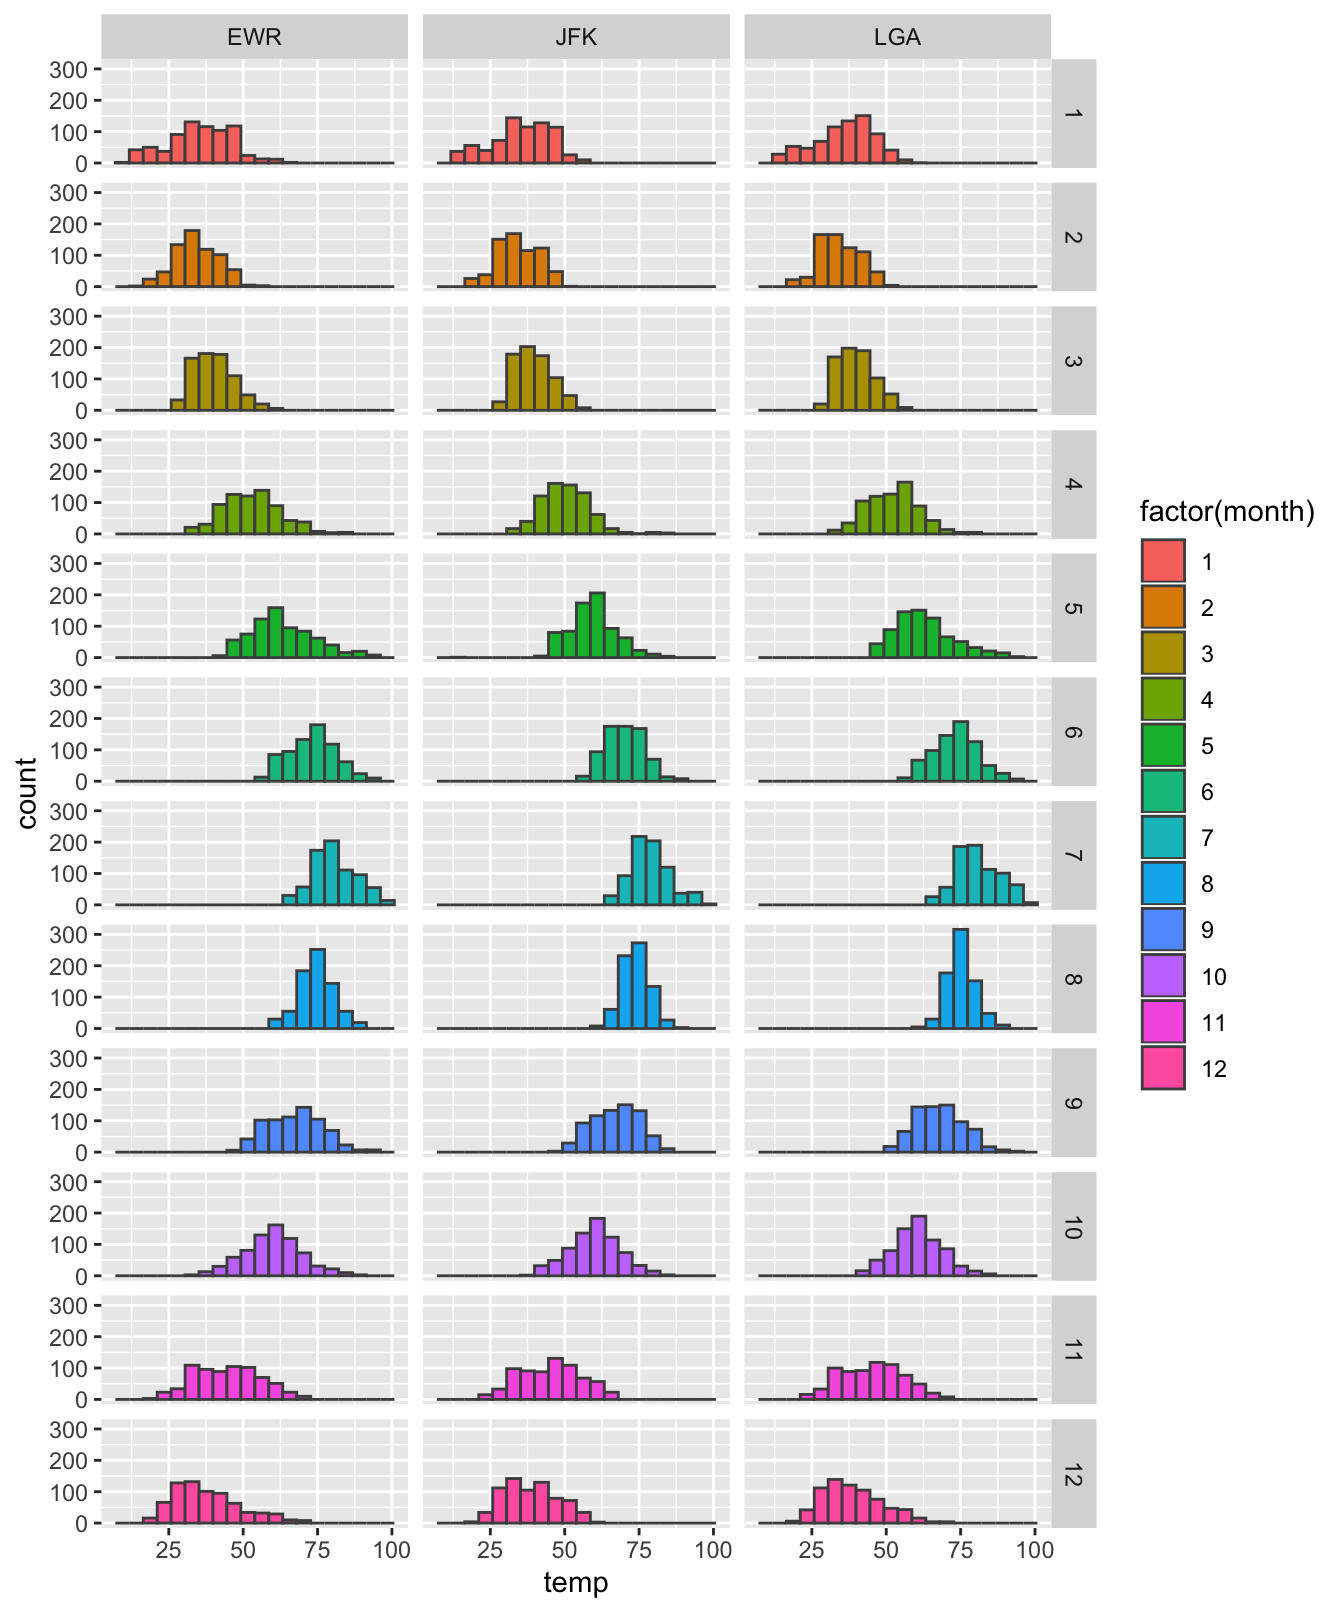
\includegraphics[width=0.9\linewidth]{figure/grid-1}

\}

\textbackslash{}caption\{Un exemple d'utilisation de
\texttt{facet\_grid()}\}\label{fig:grid} \textbackslash{}end\{figure\}

Ici, nous avons utilisé la variable \texttt{month} (transformée en
facteur) et la variable \texttt{origin} pour créer un histogramme pour
chaque combinaison des modalités de ces 2 variables. Il est donc
possible comparer facilement des températures inter-mensuelles au sein
d'un aéroport donné (en colonnes), ou de comparer des températures
enregistrées le même mois dans des aéroports distincts (en lignes).

\texttt{facet\_grid()} doit elle aussi être utilisée avec le symbole
\texttt{\textasciitilde{}}. Comme pour les indices d'un tableau, on met
à gauche du \texttt{\textasciitilde{}} la variable qui figurera en
lignes, et à droite du \texttt{\textasciitilde{}} celle qui figurera en
colonnes. Les arguments \texttt{nrow} et \texttt{ncol} ne peuvent donc
pas être utilisés : c'est le nombre de niveaux de chaque variable
catégorielle fournie à \texttt{facet\_grid()} qui détermine le nombre de
lignes et de colonnes du graphique.

Vous devriez maintenant être convaincus de la puissance de la grammaire
des graphiques. En utilisant un langage standardisé et en ajoutant des
couches une à une sur un graphique, il est posible d'obtenir rapidement
des visualisations très complexes et néanmoins très claires, qui font
apparaître des srtuctures intéressantes dans nos données (des tendances,
des groupes, des similitudes, des liaisons, des différences, etc).

\hypertarget{exercices-4}{%
\subsubsection{Exercices}\label{exercices-4}}

Examinez la figure \ref{fig:grid}.

\begin{enumerate}
\def\labelenumi{\arabic{enumi}.}
\tightlist
\item
  Quels éléments nouveaux ce graphiques nous apprend-il par rapport au
  graphique \ref{fig:break} ci-dessus ? Comment le ``\texttt{facet}ing''
  nous aide-t'il à visualiser les relations entre 2 (ou 3) variables ?
\item
  À quoi correspondent les numéros 1 à 12 ?
\item
  À quoi correspondent les chiffres 25, 50, 75, 100 ?
\item
  À quoi correspondent les chiffres 0, 100, 200, 300 ?
\item
  Observez les échelles des axes \texttt{x} et \texttt{y} pour chaque
  sous graphique. Qu'on-t'elles de particulier ? En quoi est-ce utile ?
\item
  La variabilité des températures est-elle plus importante entre les
  aéroports, entre les mois, ou au sein des mois ? Expliquez votre
  réflexion.
\end{enumerate}

\begin{center}\rule{0.5\linewidth}{\linethickness}\end{center}

\hypertarget{les-boites-a-moustaches-ou-boxplots}{%
\subsection{Les boîtes à moustaches ou
boxplots}\label{les-boites-a-moustaches-ou-boxplots}}

\hypertarget{creation-de-boxplots-et-informations-apportees}{%
\subsubsection{Création de boxplots et informations
apportées}\label{creation-de-boxplots-et-informations-apportees}}

Commençons par créer un boxplot pour comparer les températures
mensuelles comme nous l'avons fait plus haut avec des histogrammes :

\begin{Shaded}
\begin{Highlighting}[]
\KeywordTok{ggplot}\NormalTok{(weather, }\KeywordTok{aes}\NormalTok{(}\DataTypeTok{x =}\NormalTok{ month, }\DataTypeTok{y =}\NormalTok{ temp)) }\OperatorTok{+}
\StringTok{  }\KeywordTok{geom_boxplot}\NormalTok{()}
\end{Highlighting}
\end{Shaded}

\begin{verbatim}
Warning: Continuous x aesthetic -- did you forget aes(group=...)?
\end{verbatim}

\begin{verbatim}
Warning: Removed 1 rows containing non-finite values (stat_boxplot).
\end{verbatim}

\begin{figure}[htpb]

{\centering 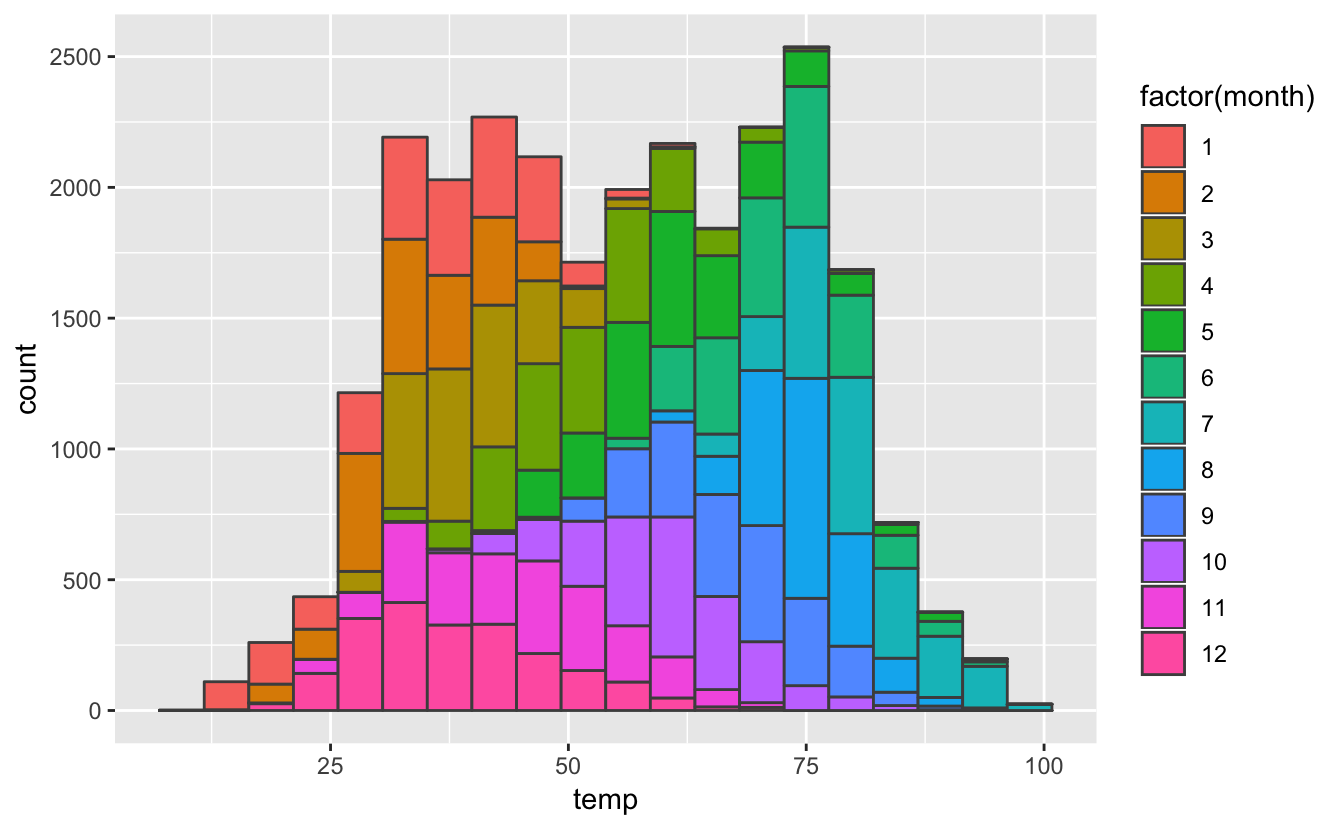
\includegraphics[width=0.9\linewidth]{figure/unnamed-chunk-54-1} 

}

\caption{Un boxplot for peu utile...}\label{fig:unnamed-chunk-54}
\end{figure}

Comme précédemment, R nous avertit qu'une observation n'a pas été
intégrée (en raison d'une donnée manquante). Mais il nous dit aussi que
\texttt{x} (pour nous, la variable \texttt{month}) est continue, et que
nous avons probablement oublié de spécifier des groupes.

En effet, les boxplots sont généralement utilisés pour examiner la
distribution d'une variable numérique pour chaque niveau d'une variable
catégorielle (un facteur). Il nous faut donc, ici encore, transformer
\texttt{month} en facteur car dans notre tableau de départ, cette
variable est considérée comme une variable numérique continue :

\begin{Shaded}
\begin{Highlighting}[]
\KeywordTok{ggplot}\NormalTok{(weather, }\KeywordTok{aes}\NormalTok{(}\DataTypeTok{x =} \KeywordTok{factor}\NormalTok{(month), }\DataTypeTok{y =}\NormalTok{ temp)) }\OperatorTok{+}
\StringTok{  }\KeywordTok{geom_boxplot}\NormalTok{()}
\end{Highlighting}
\end{Shaded}

\begin{figure}[htpb]

{\centering 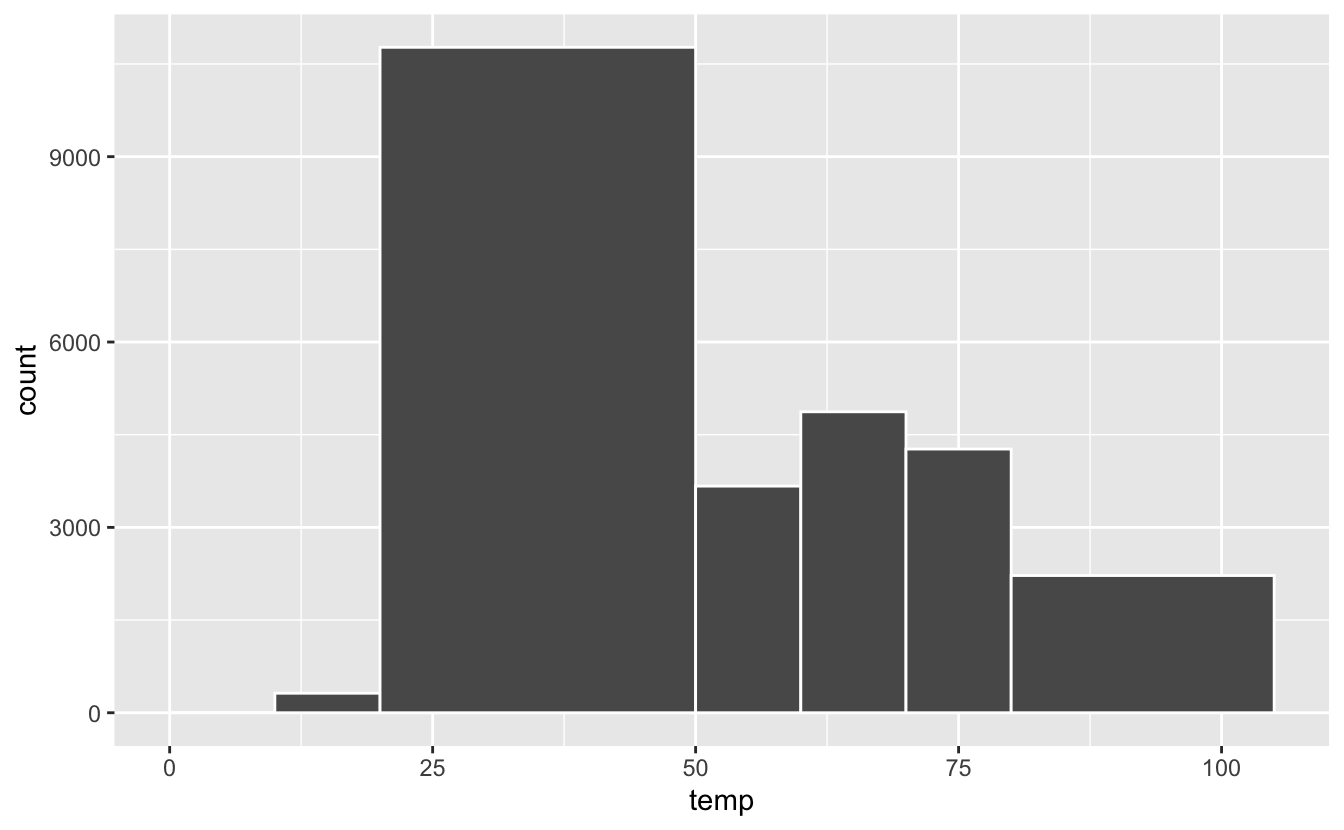
\includegraphics[width=0.9\linewidth]{figure/unnamed-chunk-55-1} 

}

\caption{Boxplot des températures mensuelles}\label{fig:unnamed-chunk-55}
\end{figure}

Les différents éléments d'un boxplot, sont les suivants :

\begin{itemize}
\tightlist
\item
  la limite inférieure de la boîte correspond au premier quartile : 25\%
  des données de l'échantillon sont situées sous cette valeur
\item
  la limite supérieure de la boîte correspond au troisième quartile :
  25\% des données de l'échantillon sont situées au-dessus de cette
  valeur
\item
  le segment épais à l'intérieur de la boîte corrspond au second
  quartile : c'est la médiane de l'échantillon. 50\% des données de
  l'échantillon sont situées au dessus de cette valeur, et 50\% au
  dessous.
\item
  la hauteur de la boîte correspond à ce que l'on appelle l'étendue
  inter-quartile ou Inter Quartile Range (IQR) en anglais. On trouve
  dans cette boîte 50\% des observations de l'échantillon. C'est une
  mesure de la dispersion des 50\% des données les plus centrales. Une
  boîte plus allongée indique donc une plus grande dispersion.
\item
  les moustaches correspondent à des valeurs qui sont en dessous du
  premier quartile (pour la moustache du bas) et au-dessus du troisième
  quartile (pour la moustache du haut). La règle utilisée dans R est que
  ces moustaches s'étendent jusqu'aux valeurs minimales et maximales de
  l'échantillon, mais elles ne peuvent en aucun cas s'étendre au-delà de
  1,5 fois la hauteur de la boîte (1,5 fois l'IQR) vers le haut et le
  bas. Si des points apparaissent au-delà des moustaches (vers le haut
  ou le bas), ces points sont appelés ``outliers''. Ce sont des points
  qui s'éloignent du centre de la distribution de façon importante
  puisqu'ils sont au-delà de 1,5 fois l'IQR de part et d'autres du
  premier ou du troisième quartile. Il peut s'agir d'anomalies de
  mesure, d'anomalies de saisie de données, ou tout simplement,
  d'enregistrement tout à fait valides mais extrêmes. J'attire votre
  attention sur le fait que la définition de ces outliers est
  relativement arbitraire. Nous pourrions faire le choix d'étendre les
  moustaches jusqu'à 1,8 fois l'IQR (ou 2, ou 2,5). Nous observerions
  alors beaucoup moins d'outliers. D'une façons générale, la longueur
  des moustaches renseigne sur la variabilité des données en dehors de
  la zone centrale. Plus elles sont longues, plus la variabilité est
  importante. Et dans tous les cas, l'examen attentif des outliers est
  utile car il nous permet d'en apprendre plus sur le comportement
  extrême de certaines observations.
\end{itemize}

\hypertarget{lintervalle-de-confiance-a-95-de-la-mediane}{%
\subsubsection{L'intervalle de confiance à 95\% de la
médiane}\label{lintervalle-de-confiance-a-95-de-la-mediane}}

On peut également aujouter une encoche autour de la valeur de médiane en
ajoutant l'argument \texttt{notch\ =\ TRUE} à la fonction
\texttt{geom\_boxplot()} :

\begin{Shaded}
\begin{Highlighting}[]
\KeywordTok{ggplot}\NormalTok{(weather, }\KeywordTok{aes}\NormalTok{(}\DataTypeTok{x =} \KeywordTok{factor}\NormalTok{(month), }\DataTypeTok{y =}\NormalTok{ temp)) }\OperatorTok{+}
\StringTok{  }\KeywordTok{geom_boxplot}\NormalTok{(}\DataTypeTok{notch =} \OtherTok{TRUE}\NormalTok{)}
\end{Highlighting}
\end{Shaded}

\textbackslash{}begin\{figure\}{[}htpb{]}

\{\centering 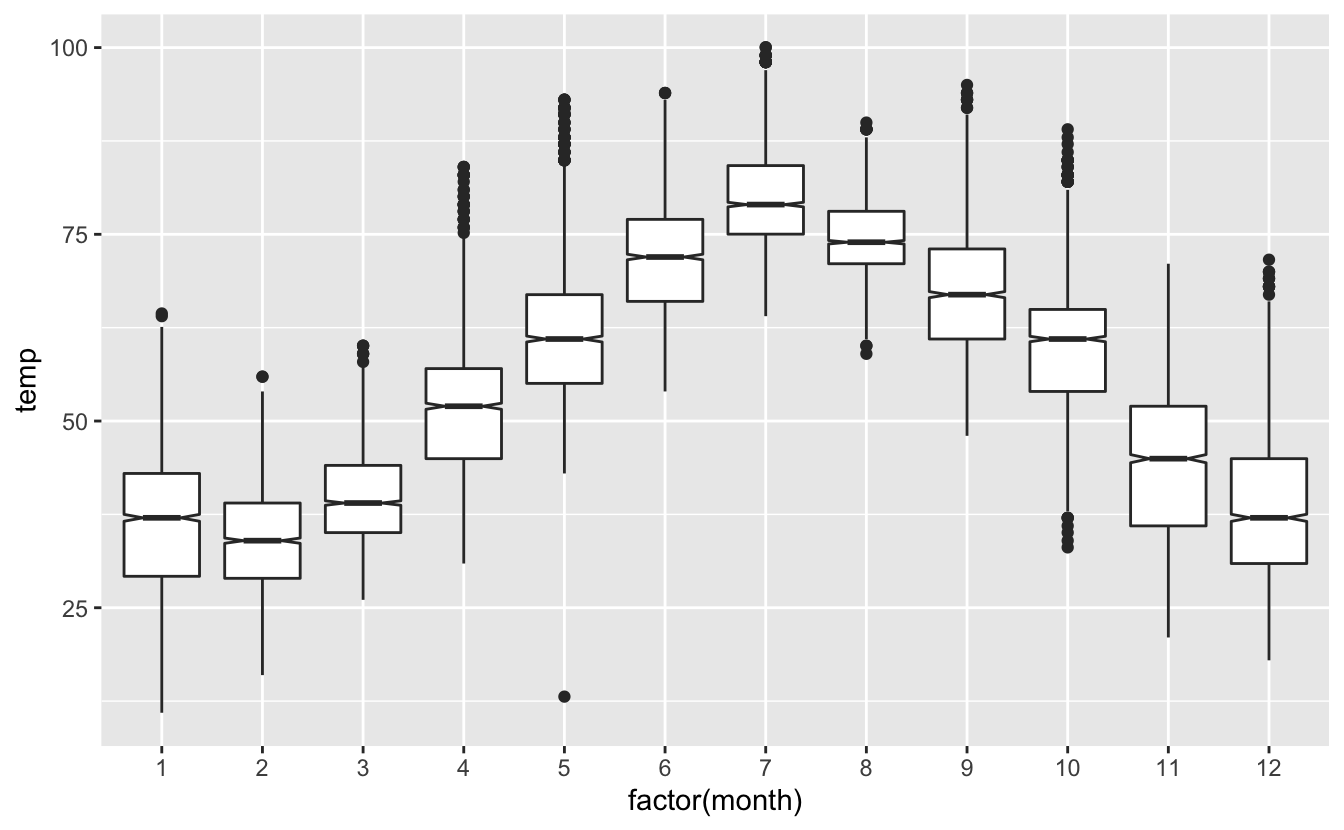
\includegraphics[width=0.9\linewidth]{figure/notchedboxplot-1}

\}

\textbackslash{}caption\{Boxplot des températures mensuelles. Les
intervalles de confiance à 95\% de la médiane sont
affichés.\}\label{fig:notchedboxplot} \textbackslash{}end\{figure\}

Comme l'indique la légende de la figure \ref{fig:notchedboxplot}, cette
encoche correspond à l'étendue de l'intervalle de confiance à 95\% de la
médiane. Pour chaque échantillon, nous espérons que la médiane calculée
soit le reflet fidèle de la vraie valeur de médiane de la population.
Mais il sera toujours impossible d'en avoir la certitude absolue. Le
mieux que l'on puisse faire, c'est quantifier l'incertitude.
L'intervalle de confiance nous indique qu'il ya de bonnes chances que la
vraie valeur de médiane de la population générale (qui restera à jamais
inconnue) a de bonnes chances de se trouver dans cet intervalle. Ici,
les encoches sont très étroites car les données sont abondantes. il y a
donc peu d'incertitude, ce qui est une bonne chose.\\
Nous reviendrons sur cette notion importante à la fin des TP de
biométrie 2 ou en biométrie 3, car ce type de graphique nous permettra
d'anticiper sur les résultats des tests de comparaison de moyennes.

\hypertarget{une-autre-facon-dexaminer-des-distributions}{%
\subsubsection{Une autre façon d'examiner des
distributions}\label{une-autre-facon-dexaminer-des-distributions}}

Dernière chose concernant les boxplots : il s'agit d'une représentation
graphique très proche de l'histogramme. Pour vous en convaincre, je
représente à la figure \ref{fig:compboxplot} ci-dessous uniquement les
temperatures du mois de novembre, avec 3 types d'objets géométriques
différents : un histogramme, un boxplot, et un nuage de points.

\begin{figure}[htpb]

{\centering 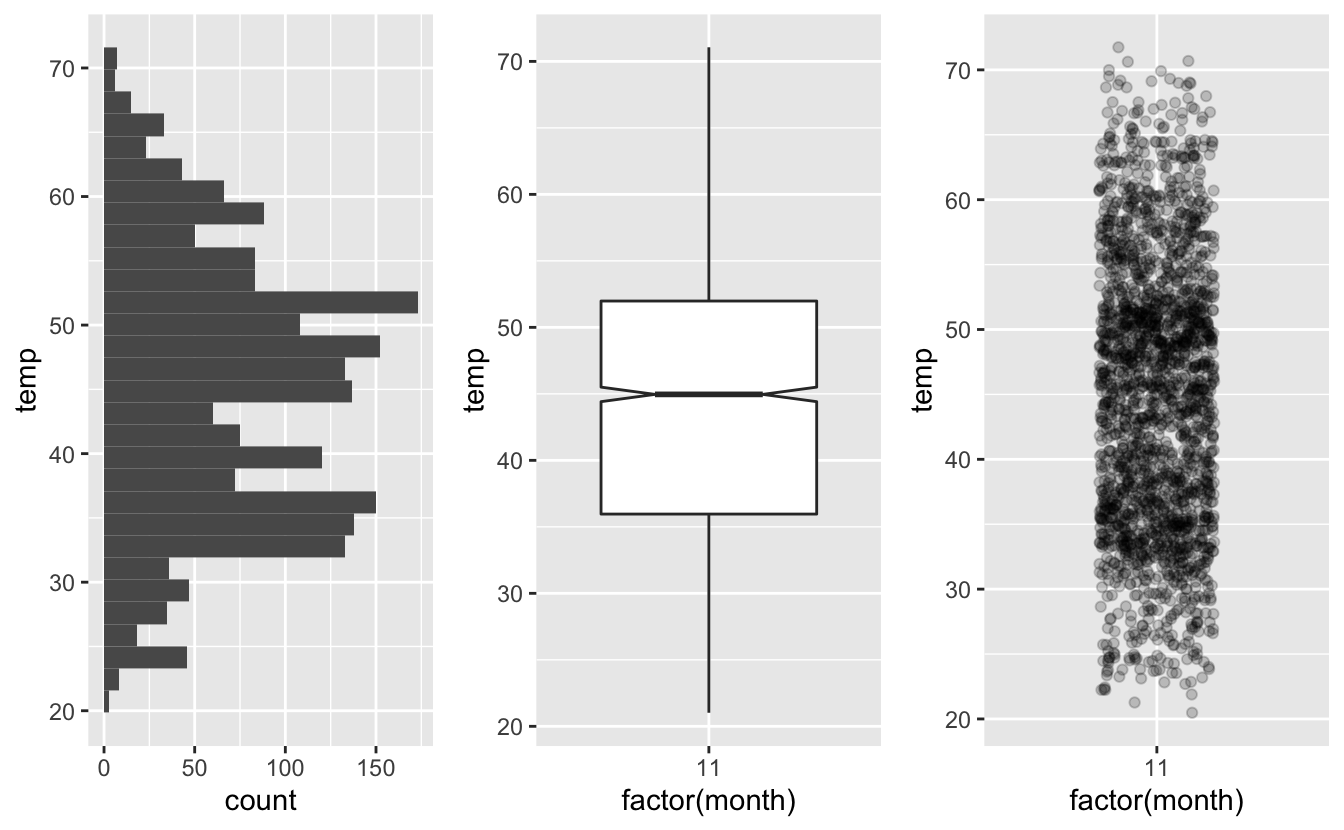
\includegraphics[width=0.9\linewidth]{figure/compboxplot-1} 

}

\caption{Distribution des températures de Novembre 2013}\label{fig:compboxplot}
\end{figure}

Nous avons donc, à gauche un histogramme pour les températures de
novembre (j'ai permuté les axes pour que \texttt{y} porte la température
pour les 3 graphiques), au centre, un boxplot pour ces mêmes données, et
à droite, les données brutes, sous la forme d'un nuage de point créé
avec \texttt{geom\_jitter()}. On voit bien que ces 3 représentations
graphiques sont similaires. Toutes rendent compte du fait que les
températures de Novembre sont majoritairement comprises entre 35 et 52
degrés farenheit. Au-delà de cette fourchette (au-dessus comme
en-dessous) les observations sont plus rares.

Le nuage de points affiche toutes les données. C'est donc lui le plus
complet mais pas forcément le plus lisible. Les points sont en effet
très nombreux et la lecture du graphique peut s'en trouver compliquée.
L'histogramme simplifie les données en les regroupant dans des classes.
C'est une sorte de résumé des données. On constate cependant toujours la
présence de 2 pics qui correspondent aux zones plus denses du nuage de
points. Le boxplot enfin synthétise encore plus ces données. Elles sont
résumées par 7 valeurs seulement : le minimum, le maximum, les 3
quartiles, et les bornes de l'intervalle de confiance à 95\% de la
médiane. C'est une représentation très synthétique qui nous permet de
comparer beaucoup de catégories côte à côte (voir la figure
\ref{fig:notchedboxplot} un peu plus haut), mais qui est forcément moins
précise qu'un histogramme. Vous noterez toutefois que la boîte du
boxplot recouvre en grande partie la zone des 2 pics de l'histogramme.
En outre, sur la figure \ref{fig:notchedboxplot}, la tendance générale
est très visible : il fait plus chaud en été qu'en hiver (étonnant non
?).

\hypertarget{pour-conclure}{%
\subsubsection{Pour conclure}\label{pour-conclure}}

Les boîtes à moustaches permettent donc de comparer et contraster la
distribution d'\textbf{une variable quantitative} pour plusieurs niveaux
d'\textbf{une variable catégorielle}. On peut voir où la médiane tombe
dans les différents groupes en observant la position de la ligne
centrale dans la boîte. Pour avoir une idée de la dispersion de la
variable au sein de chaque groupe, regardez à la fois la hauteur de la
boîte et la longueur des moustaches. Quand les moustaches s'étendent
loin de la boîte mais que la boîte est petite, cela signifie que la
variabilité des valeurs proches du centre de la distribution est
beaucoup plus faible que la variabilité des valeurs extrêmes. Enfin, les
valeurs extrêmes ou aberrantes sont encore plus faciles à détecter avec
une boîte à moustaches qu'avec un histogramme.

\begin{center}\rule{0.5\linewidth}{\linethickness}\end{center}

\hypertarget{les-diagrammes-batons}{%
\subsection{Les diagrammes bâtons}\label{les-diagrammes-batons}}

Comme nous venons de le voir, les histogrammes et les boîtes à
moustaches permettent de visualiser la distribution d'une
\textbf{variable numérique continue}. Nous aurons aussi souvent besoin
de visualiser la distribution d'une \textbf{variable catégorielle}.
C'est une tâche plus simple qui consiste à compter combien d'éléments
tombent dans chacune des catégories de la variable catégorielle. Le
meilleur moyen de visualiser de telles données de comptage (\emph{aka}
fréquences) est de réaliser un diagramme bâtons, autrement appelé
\textbf{barplot} ou \textbf{barchart}.

Une difficulté, toutefois, concerne la façon dont les données sont
présentées : est-ce que la variable d'intérêt est ``pré-comptée'' ou non
? Par exemple, le code ci-dessous crée 2 \texttt{data.frame} qui
représentent la même collection de fruits : 3 pommes et 2 oranges :

\begin{Shaded}
\begin{Highlighting}[]
\NormalTok{fruits <-}\StringTok{ }\KeywordTok{data_frame}\NormalTok{(}\DataTypeTok{fruit =} \KeywordTok{c}\NormalTok{(}\StringTok{"pomme"}\NormalTok{, }\StringTok{"pomme"}\NormalTok{, }\StringTok{"pomme"}\NormalTok{, }\StringTok{"orange"}\NormalTok{, }\StringTok{"orange"}\NormalTok{))}
\NormalTok{fruits}
\end{Highlighting}
\end{Shaded}

\begin{verbatim}
# A tibble: 5 x 1
  fruit 
  <chr> 
1 pomme 
2 pomme 
3 pomme 
4 orange
5 orange
\end{verbatim}

\begin{Shaded}
\begin{Highlighting}[]
\NormalTok{fruits_counted <-}\StringTok{ }\KeywordTok{data_frame}\NormalTok{(}\DataTypeTok{fruit =} \KeywordTok{c}\NormalTok{(}\StringTok{"pomme"}\NormalTok{, }\StringTok{"orange"}\NormalTok{), }\DataTypeTok{nombre =} \KeywordTok{c}\NormalTok{(}\DecValTok{3}\NormalTok{, }\DecValTok{2}\NormalTok{))}
\NormalTok{fruits_counted}
\end{Highlighting}
\end{Shaded}

\begin{verbatim}
# A tibble: 2 x 2
  fruit  nombre
  <chr>   <dbl>
1 pomme       3
2 orange      2
\end{verbatim}

\hypertarget{representation-graphique-avec-geom_bar-et-geom_col}{%
\subsubsection{\texorpdfstring{Représentation graphique avec
\texttt{geom\_bar} et
\texttt{geom\_col}}{Représentation graphique avec geom\_bar et geom\_col}}\label{representation-graphique-avec-geom_bar-et-geom_col}}

Pour visualiser les données non pré-comptées, on utilise
\texttt{geom\_bar()} :

\begin{Shaded}
\begin{Highlighting}[]
\KeywordTok{ggplot}\NormalTok{(}\DataTypeTok{data =}\NormalTok{ fruits, }\DataTypeTok{mapping =} \KeywordTok{aes}\NormalTok{(}\DataTypeTok{x =}\NormalTok{ fruit)) }\OperatorTok{+}
\StringTok{  }\KeywordTok{geom_bar}\NormalTok{()}
\end{Highlighting}
\end{Shaded}

\begin{figure}[htpb]

{\centering 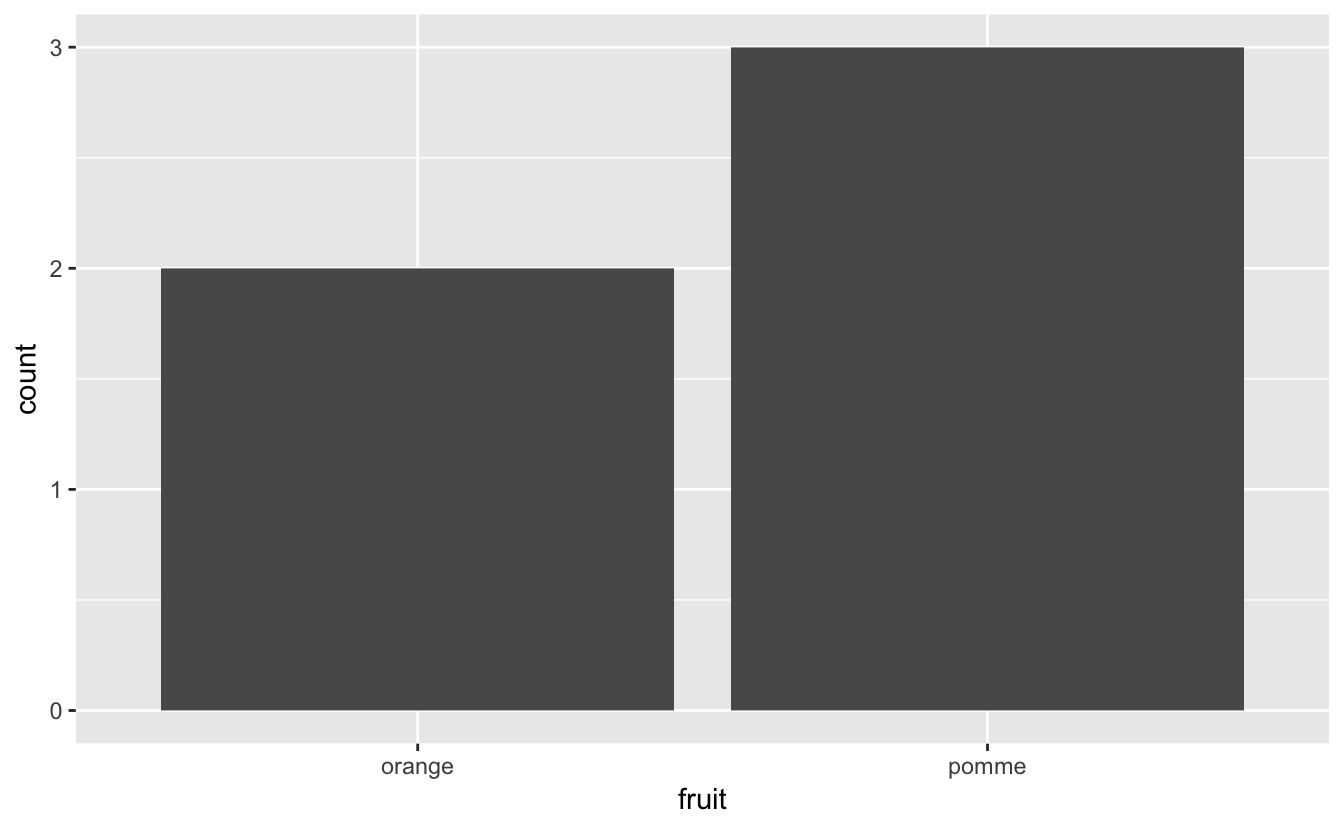
\includegraphics[width=0.9\linewidth]{figure/barplot-1} 

}

\caption{Barplot pour des données non pré-comptées.}\label{fig:barplot}
\end{figure}

Pour visualiser les données déjà pré-comptées, on utilise
\texttt{geom\_col()} :

\begin{Shaded}
\begin{Highlighting}[]
\KeywordTok{ggplot}\NormalTok{(}\DataTypeTok{data =}\NormalTok{ fruits_counted, }\DataTypeTok{mapping =} \KeywordTok{aes}\NormalTok{(}\DataTypeTok{x =}\NormalTok{ fruit, }\DataTypeTok{y =}\NormalTok{ nombre)) }\OperatorTok{+}
\StringTok{  }\KeywordTok{geom_col}\NormalTok{()}
\end{Highlighting}
\end{Shaded}

\begin{figure}[htpb]

{\centering 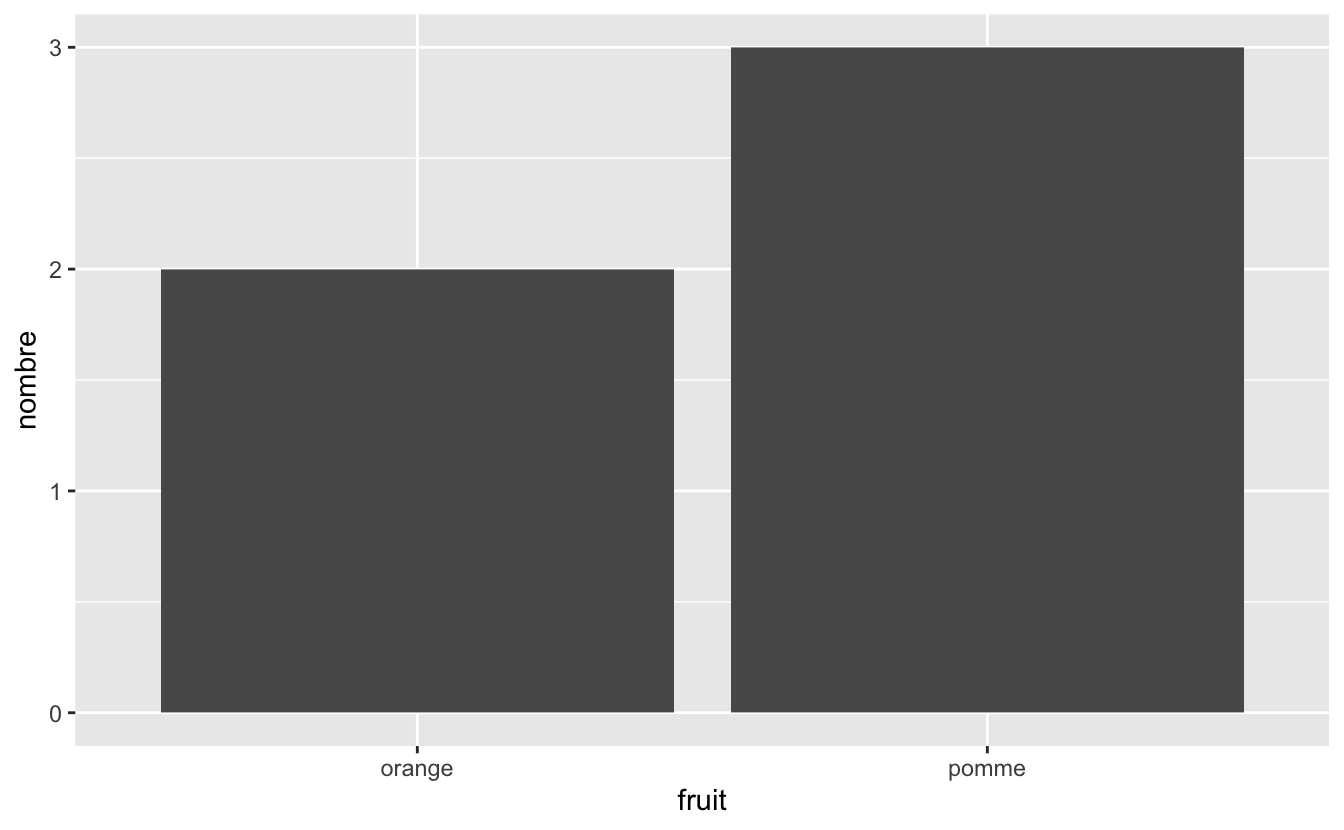
\includegraphics[width=0.9\linewidth]{figure/barplotcol-1} 

}

\caption{Barplot pour des données pré-comptées.}\label{fig:barplotcol}
\end{figure}

Notez que les figures \ref{fig:barplot} et \ref{fig:barplotcol} sont
absolument identiques (à l'exception du titre de l'axe des ordonnées),
mais qu'elles ont été créées à partir de 2 tableaux de données
différents. En particulier, notez que :

\begin{itemize}
\tightlist
\item
  le code qui génère la figure \ref{fig:barplot} utilise le jeu de
  données \texttt{fruits}, et n'associe pas de variable à l'axe des
  ordonnées : dans la fonction \texttt{aes()}, seule la variable
  associée à \texttt{x} est précisée. C'est la fonction
  \texttt{geom\_bar()} qui calcule automatiquement les abondances (ou
  fréquences) pour chaque catégorie de la variable \texttt{fruit}. La
  variable \texttt{count} est ainsi générée automatiquement et associée
  à \texttt{y}.
\item
  le code qui génère la figure \ref{fig:barplotcol} utilise le jeu de
  données \texttt{fruits\_counted}. Ici, la variable \texttt{nombre} est
  associée à l'axe des \texttt{y} grâce à la fonction \texttt{aes()}. La
  fonction \texttt{geom\_col()} a besoin de 2 variables (une variable
  catégorielle pour l'axe des \texttt{x} et une numérique pour l'axe des
  \texttt{y}) pour fonctionner.
\end{itemize}

Autrement dit, lorsque vous souhaiterez créer un diagramme bâtons, il
faudra donc au préalable vérifier de quel type de données vous disposez
pour choisir l'objet géométrique approprié :

\begin{itemize}
\tightlist
\item
  Si votre variable catégorielle n'est pas pré-comptée dans votre
  tableau de données, il faut utiliser \texttt{geom\_bar()}
\item
  Si votre variable catégorielle est pré-comptée dans votre tableau de
  données, il faut utiliser \texttt{geom\_col()} et associer
  explicitement les comptages à l'aesthétique \texttt{y} du graphique.
\end{itemize}

\hypertarget{un-example-concret}{%
\subsubsection{Un example concret}\label{un-example-concret}}

Revenons à \texttt{nycflights13}. Imaginons que nous souhaitions
connaître le nombre de vols affrétés par chaque compagnie aérienne au
départ de New York en 2013. Dans le jeu de données \texttt{flights}, la
variable \texttt{carrier} nous indique à quelle compagnie aérienne
appartiennent chacun des 336776 vols ayant quitté New York en 2013. Une
façon simple de représenter ces données est donc la suivante :

\begin{Shaded}
\begin{Highlighting}[]
\KeywordTok{ggplot}\NormalTok{(}\DataTypeTok{data =}\NormalTok{ flights, }\DataTypeTok{mapping =} \KeywordTok{aes}\NormalTok{(}\DataTypeTok{x =}\NormalTok{ carrier)) }\OperatorTok{+}
\StringTok{  }\KeywordTok{geom_bar}\NormalTok{()}
\end{Highlighting}
\end{Shaded}

\begin{figure}[htpb]

{\centering 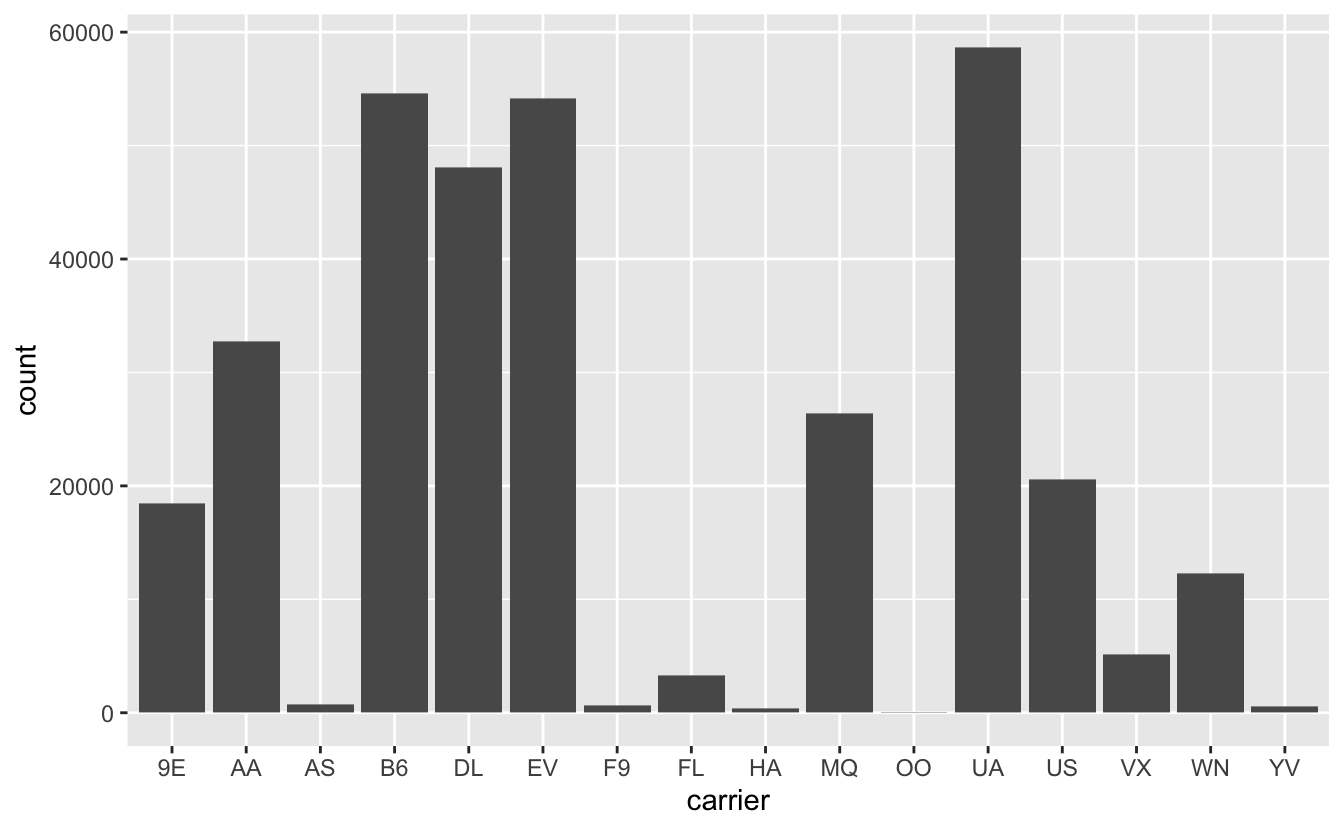
\includegraphics[width=0.9\linewidth]{figure/bpcarrier-1} 

}

\caption{Nombre de vols par compagnie aérienne au départ de New York en 2013.}\label{fig:bpcarrier}
\end{figure}

Ici, \texttt{geom\_bar()} a compté le nombre d'occurences de chaque
compagnie aérienne dans le tableau \texttt{flights} et a automatiquement
associé ce nombre à l'axe des ordonnées.

Il est généralement plus utile de trier les catégories par ordre
décroissant. Nous pouvons faire cela facilement grâce à la fonction
\texttt{fct\_infreq()} du package \texttt{forcats}. Si vous avez
installé le \texttt{tidyverse}, le package \texttt{forcast} doit être
disponible sur votre ordinateur. N'oubliez pas de le charger si besoin :

\begin{Shaded}
\begin{Highlighting}[]
\KeywordTok{library}\NormalTok{(forcats)}
\KeywordTok{ggplot}\NormalTok{(}\DataTypeTok{data =}\NormalTok{ flights, }\DataTypeTok{mapping =} \KeywordTok{aes}\NormalTok{(}\DataTypeTok{x =} \KeywordTok{fct_infreq}\NormalTok{(carrier))) }\OperatorTok{+}
\StringTok{  }\KeywordTok{geom_bar}\NormalTok{()}
\end{Highlighting}
\end{Shaded}

\begin{figure}[htpb]

{\centering 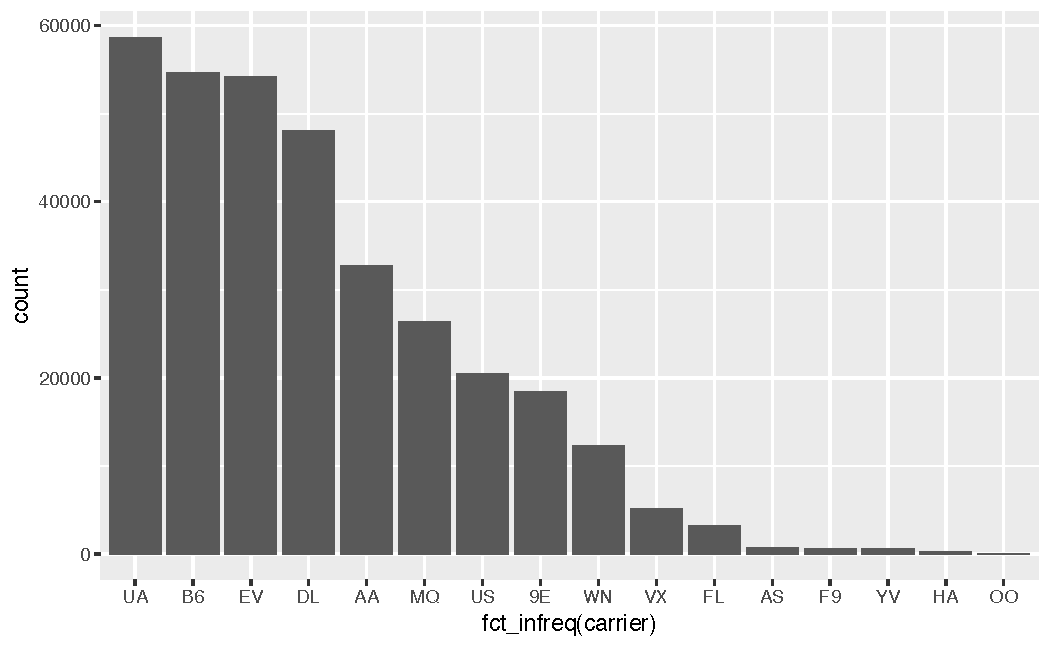
\includegraphics[width=0.9\linewidth]{figure/bpcarriersorted-1} 

}

\caption{Nombre de vols par compagnie aérienne au départ de New York en 2013.}\label{fig:bpcarriersorted}
\end{figure}

Ordonner les catégories par ordre décroissant est souvent indispensable
afin de faciliter la lecture du graphique et les comparaisons entre
catégories.

Si nous souhaitons connaître le nombre de vols précis de chaque
compagnie aérienne, il nous faut faire appel à plusieurs fonctions du
package \texttt{dplyr} que nous détaillerons dans le chapitre
\ref{wrangling}. Ci-dessous, nous créons un nouveau tableau
\texttt{carrier\_table} contenant le nombre de vols de chaque compagnie
aérienne et les compagnies sont ordonnées par nombre de vols
décroissants :

\begin{Shaded}
\begin{Highlighting}[]
\NormalTok{carrier_table <-}\StringTok{ }\NormalTok{flights }\OperatorTok\StringTok{   }\CommentTok{# Pour créer une nouvelle table, on prend flights, puis...}
\StringTok{  }\KeywordTok{group_by}\NormalTok{(carrier) }\OperatorTok\StringTok{        }\CommentTok{# On groupe les données par compagnie aérienne, puis...}
\StringTok{  }\KeywordTok{summarize}\NormalTok{(}\DataTypeTok{nombre =} \KeywordTok{n}\NormalTok{()) }\OperatorTok\StringTok{  }\CommentTok{# On calcule le nombre de vols par compagnie, puis ...}
\StringTok{  }\KeywordTok{arrange}\NormalTok{(}\KeywordTok{desc}\NormalTok{(nombre))        }\CommentTok{# On trie le tableau par nombre de vols décroissant.}
\NormalTok{carrier_table                  }\CommentTok{# Enfin, on affiche la nouvelle table}
\end{Highlighting}
\end{Shaded}

\begin{verbatim}
# A tibble: 16 x 2
   carrier nombre
   <chr>    <int>
 1 UA       58665
 2 B6       54635
 3 EV       54173
 4 DL       48110
 5 AA       32729
 6 MQ       26397
 7 US       20536
 8 9E       18460
 9 WN       12275
10 VX        5162
11 FL        3260
12 AS         714
13 F9         685
14 YV         601
15 HA         342
16 OO          32
\end{verbatim}

Ici, la table a été triée par nombre de vols décroissants. Mais
attention, \textbf{les niveaux} du facteur \texttt{carrier} n'ont pas
été modifiés :

\begin{Shaded}
\begin{Highlighting}[]
\KeywordTok{factor}\NormalTok{(carrier_table}\OperatorTok{$}\NormalTok{carrier)}
\end{Highlighting}
\end{Shaded}

\begin{verbatim}
 [1] UA B6 EV DL AA MQ US 9E WN VX FL AS F9 YV HA OO
Levels: 9E AA AS B6 DL EV F9 FL HA MQ OO UA US VX WN YV
\end{verbatim}

Le premier niveau est toujours \texttt{9E}, puis \texttt{AA}, puis
\texttt{AS}, et non l'ordre du tableau nouvellement créé (\texttt{UA},
puis \texttt{B6}, puis \texttt{EV}\ldots{}) car les niveaux sont
toujours triés par ordre alphabétique. La conséquence est que faire un
barplot avec ces données et la fonction \texttt{geom\_col()} ne permet
pas d'ordonner les catégories correctement :

\begin{Shaded}
\begin{Highlighting}[]
\KeywordTok{ggplot}\NormalTok{(carrier_table, }\KeywordTok{aes}\NormalTok{(}\DataTypeTok{x =}\NormalTok{ carrier, }\DataTypeTok{y =}\NormalTok{ nombre)) }\OperatorTok{+}
\StringTok{  }\KeywordTok{geom_col}\NormalTok{()}
\end{Highlighting}
\end{Shaded}

\begin{figure}[htpb]

{\centering 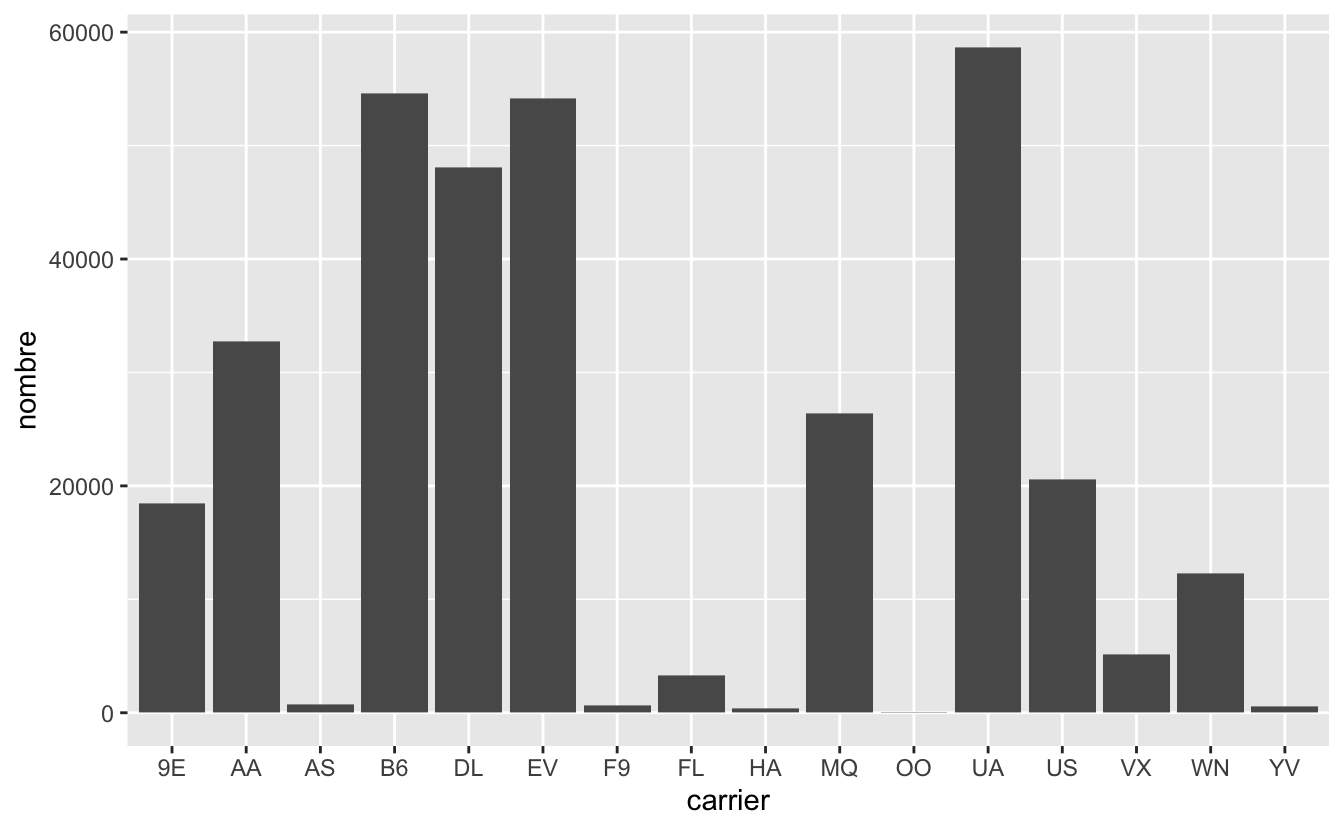
\includegraphics[width=0.9\linewidth]{figure/bpcarriercol-1} 

}

\caption{Nombre de vols par compagnie aérienne au départ de New York en 2013.}\label{fig:bpcarriercol}
\end{figure}

Pour parvenir à nos fins, il faut cette fois avoir recours à la fonction
\texttt{fct\_reorder()} pour ordonner correctement les catégories. Cette
fonction prends 3 arguments :

\begin{enumerate}
\def\labelenumi{\arabic{enumi}.}
\tightlist
\item
  la variable catégorielle dont on souhaite réordonner les niveaux (ici,
  la variable \texttt{carrier} du tableau \texttt{carrier\_table})
\item
  une variable numérique qui permet d'ordonner les catégories (ici, la
  variable \texttt{nombre} du même tableau)
\item
  l'argument optionnel \texttt{.desc} qui permet de préciser si le tri
  doit être fait en ordre croissant (c'est le cas par défaut) ou
  décroissant.
\end{enumerate}

\begin{Shaded}
\begin{Highlighting}[]
\KeywordTok{ggplot}\NormalTok{(carrier_table, }\KeywordTok{aes}\NormalTok{(}\DataTypeTok{x =} \KeywordTok{fct_reorder}\NormalTok{(carrier, nombre, }\DataTypeTok{.desc =} \OtherTok{TRUE}\NormalTok{), }\DataTypeTok{y =}\NormalTok{ nombre)) }\OperatorTok{+}
\StringTok{  }\KeywordTok{geom_col}\NormalTok{()}
\end{Highlighting}
\end{Shaded}

\begin{figure}[htpb]

{\centering 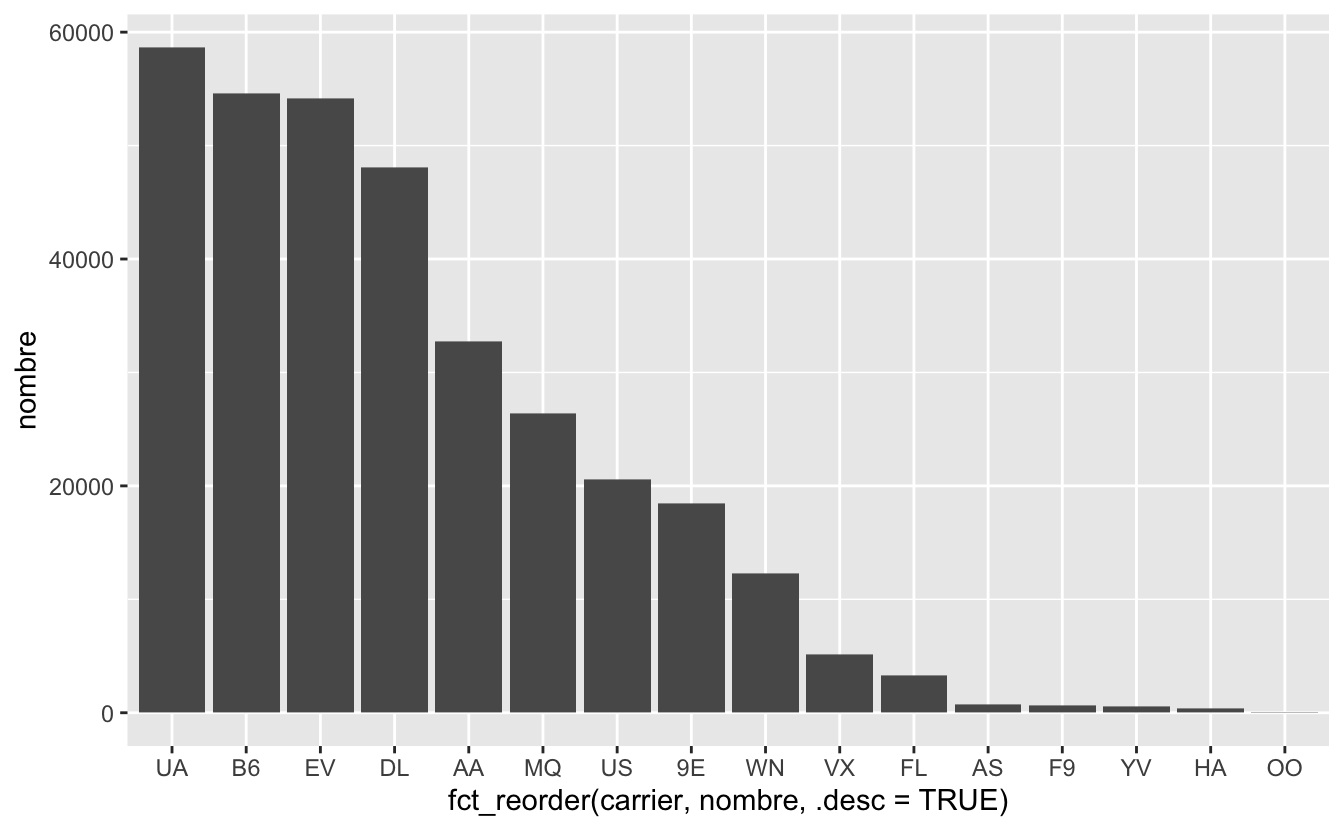
\includegraphics[width=0.9\linewidth]{figure/bpcarriersortedcol-1} 

}

\caption{Nombre de vols par compagnie aérienne au départ de New York en 2013.}\label{fig:bpcarriersortedcol}
\end{figure}

Vous voyez donc que selon le type de données dont vous disposez (soit un
tableau comme \texttt{flights}, avec toutes les observations, soit un
tableau beaucou plus compact comme \texttt{carrier\_table}), la démarche
permettant de produire un diagramme bâton, dans lequel les catégories
seront triées, sera différente.

\hypertarget{exercices-5}{%
\subsubsection{Exercices}\label{exercices-5}}

\begin{enumerate}
\def\labelenumi{\arabic{enumi}.}
\tightlist
\item
  Quelle est la différence entre un histogramme et un diagramme bâtons ?
\item
  Pourquoi les histogrammes sont-ils inadaptés pour visualiser des
  données catégorielles ?
\item
  Quel est le nom de la companie pour laquelle le plus grand nombre de
  vols ont quitté New York en 2013 (je veux connaître son nom, pas juste
  son code) ? Où se trouve cette information ?
\item
  Quel est le nom de la companie pour laquelle le plus petit nombre de
  vols ont quitté New York en 2013 (je veux connaître son nom, pas juste
  son code) ? Où se trouve cette information ?
\end{enumerate}

\hypertarget{eviter-a-tout-prix-les-diagrammes-circulaires}{%
\subsubsection{Éviter à tout prix les diagrammes
circulaires}\label{eviter-a-tout-prix-les-diagrammes-circulaires}}

À mon grand désarroi, l'un des graphiques les plus utilisé pour
représenter la distribution d'une variable catégorielle est le diagramme
circulaire (ou diagramme camembert, ou piechart en anglais). C'est
presque toujours la plus mauvaise visualisation possible. Je vous
demande de l'éviter à tout prix. Notre cerveau n'est en effet pas
correctement équipé pour comparer des angles. Ainsi, par exemple, nous
avons naturellement tendance à surestimer les angles supérieurs à 90º,
et à sous-estimer les angles inférieurs à 90º. En d'autres termes, il
est difficile pour les humains de comparer des grandeurs sur des
diagrammes circulaires.

À titre d'exemple, examinez ce diagramme, qui reprend les même chiffres
que précédemment, et tentez de répondre aux questions suivantes :

\begin{figure}[htpb]

{\centering 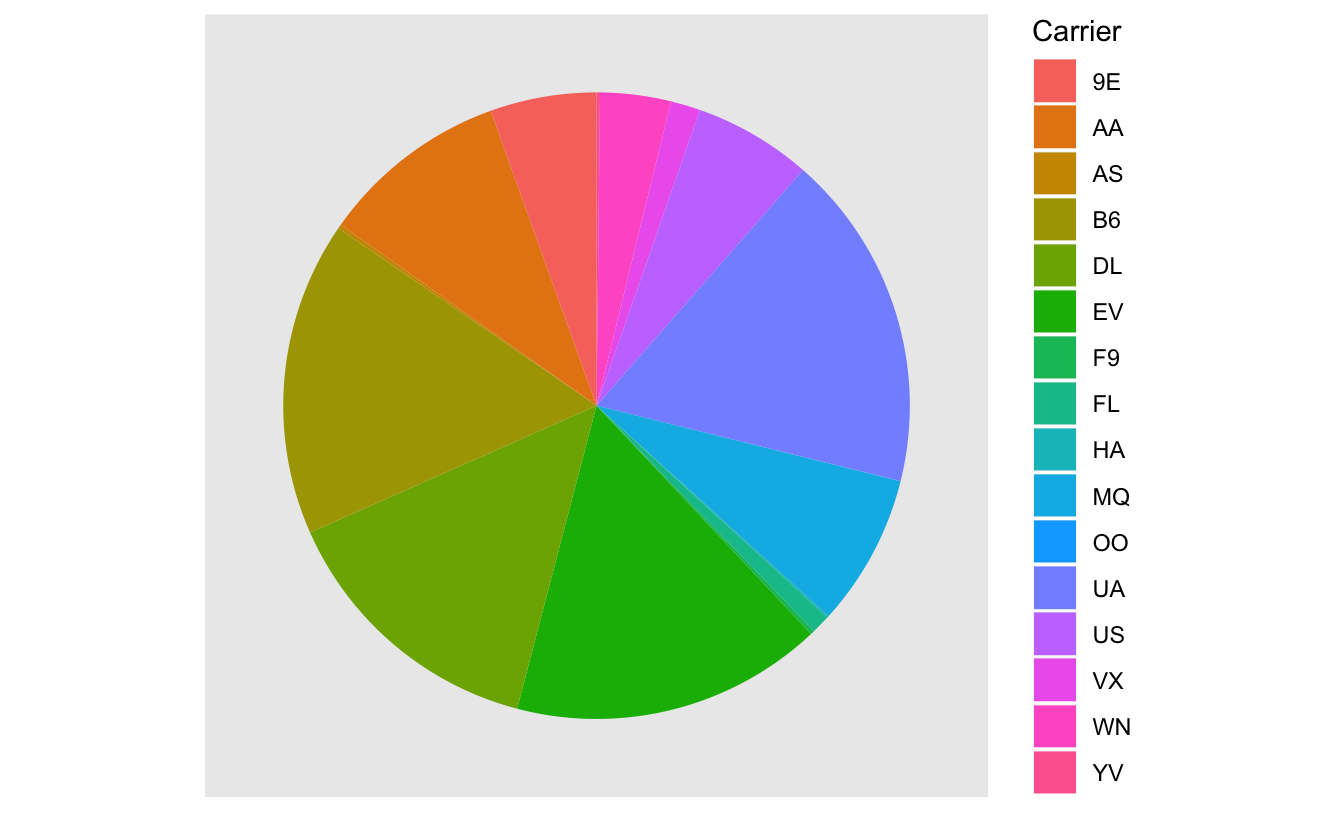
\includegraphics[width=0.9\linewidth]{figure/piechart-1} 

}

\caption{Nombre de vols par compagnie aérienne au départ de New York en 2013}\label{fig:piechart}
\end{figure}

\begin{itemize}
\tightlist
\item
  Comparez les compagnies ExpressJet Airlines (\texttt{EV}) et US
  Airways (\texttt{US}). De combien de fois la part de \texttt{EV}
  est-elle supérieure à celle d'\texttt{US} ? (2 fois, 3 fois, 1.2 fois
  ?\ldots{})
\item
  Quelle est la troisième compagnie aérienne la plus importante en terme
  de nombre de vols au départ de New York en 2013 ?
\item
  Combien de companies aériennes ont moins de vols que United Airlines
  (\texttt{UA}) ?
\end{itemize}

Il est difficile (voir impossible) de répondre précisément à ces
questions avec le diagramme circulaire de la figure \ref{fig:piechart},
alors qu'il est très simple d'obtenir des réponses précises avec un
diagramme bâtons tel que présenté à la figure
\ref{fig:bpcarriersortedcol} (vérifiez-le !).

\hypertarget{comparer-2-variables-categorielles-avec-un-diagramme-baton}{%
\subsubsection{Comparer 2 variables catégorielles avec un diagramme
bâton}\label{comparer-2-variables-categorielles-avec-un-diagramme-baton}}

Il y a généralement 3 façons de procéder pour comparer la distribution
de 2 variables catégorielles avec un diagramme bâtons :

\begin{enumerate}
\def\labelenumi{\arabic{enumi}.}
\tightlist
\item
  Faire un graphique empilé
\item
  Faire un graphique juxtaposé
\item
  Utiliser les \texttt{facet}s
\end{enumerate}

Supposons par exemple que nous devions visualiser le nombre de vol de
chaque compagnie aérienne, au départ de chacun des 3 aéroports de New
York : John F. Kennedy (\texttt{JFK}), Newark (\texttt{EWR}) et La
Guardia (LGA).

\hypertarget{graphique-empile}{%
\paragraph{Graphique empilé}\label{graphique-empile}}

La méthode la plus simple est celle du graphique empilé :

\begin{Shaded}
\begin{Highlighting}[]
\KeywordTok{ggplot}\NormalTok{(flights, }\KeywordTok{aes}\NormalTok{(}\DataTypeTok{x =} \KeywordTok{fct_infreq}\NormalTok{(carrier), }\DataTypeTok{fill =}\NormalTok{ origin)) }\OperatorTok{+}
\StringTok{  }\KeywordTok{geom_bar}\NormalTok{()}
\end{Highlighting}
\end{Shaded}

\begin{figure}[htpb]

{\centering \includegraphics[width=0.9\linewidth]{figure/stacked-1} 

}

\caption{Nombre de vols par compagnie aérienne au départ des 3 aéroports de New York en 2013.}\label{fig:stacked}
\end{figure}

Notez qu'il s'agit du même code que celui utilisé pour la figure
\ref{fig:bpcarriersorted}, à une différence près : l'ajout de
\texttt{fill\ =\ origin} dans la fonction \texttt{aes()}, qui permet
d'associer l'aéroport d'origine à la couleur de remplissage des barres.
\texttt{fill} est associé à une variable (ici, elle est catégorielle),
il est donc indispensable de faire figurer cet argument à l'intérieur de
la fonction \texttt{aes()}. Quand on associe une variable à une
caractéristique esthétique du graphique, on fait toujours figurer le
code à l'intérieur de la fonction \texttt{aes()} (comme quand on associe
une variable aux axes du graphique par exemple).

À mon sens, le graphique peut gagner en lisibilité si on ajoute une
couleur pour le contour des barres :

\begin{Shaded}
\begin{Highlighting}[]
\KeywordTok{ggplot}\NormalTok{(flights, }\KeywordTok{aes}\NormalTok{(}\DataTypeTok{x =} \KeywordTok{fct_infreq}\NormalTok{(carrier), }\DataTypeTok{fill =}\NormalTok{ origin)) }\OperatorTok{+}
\StringTok{  }\KeywordTok{geom_bar}\NormalTok{(}\DataTypeTok{color =} \StringTok{"black"}\NormalTok{)}
\end{Highlighting}
\end{Shaded}

\begin{figure}[htpb]

{\centering \includegraphics[width=0.9\linewidth]{figure/stacked2-1} 

}

\caption{Nombre de vols par compagnie aérienne au départ des 3 aéroports de New York en 2013.}\label{fig:stacked2}
\end{figure}

Notez que contrairement à \texttt{fill}, cette couleur de countour est
un paramètre fixe : elle n'est pas associée à une variable et doit donc
être placée en dehors de la fonction \texttt{aes()}.

Bien que ces graphiques empilés soient très simples à réaliser, ils sont
parfois difficiles à lire. En particulier, il n'est pas toujours aisé de
comparer les hauteurs des différentes couleurs (qui correspondent ici
aux nombres de vols issus de chaque aéroport) entre barres différentes
(qui correspondent ici aux compagnies aériennes).

\hypertarget{graphique-juxtapose}{%
\paragraph{Graphique juxtaposé}\label{graphique-juxtapose}}

Une variation sur le même thème consiste, non plus à empiler les barres
de couleur les unes sur les autres, mais à les juxtaposer :

\begin{Shaded}
\begin{Highlighting}[]
\KeywordTok{ggplot}\NormalTok{(flights, }\KeywordTok{aes}\NormalTok{(}\DataTypeTok{x =} \KeywordTok{fct_infreq}\NormalTok{(carrier), }\DataTypeTok{fill =}\NormalTok{ origin)) }\OperatorTok{+}
\StringTok{  }\KeywordTok{geom_bar}\NormalTok{(}\DataTypeTok{color =} \StringTok{"black"}\NormalTok{, }\DataTypeTok{position =} \StringTok{"dodge"}\NormalTok{)}
\end{Highlighting}
\end{Shaded}

\begin{figure}[htpb]

{\centering \includegraphics[width=0.9\linewidth]{figure/dodge-1} 

}

\caption{Nombre de vols par compagnie aérienne au départ des 3 aéroports de New York en 2013.}\label{fig:dodge}
\end{figure}

Passer d'un graphique empilé à un graphique juxtaposé est donc très
simple : il suffit d'ajouter l'argument \texttt{position\ =\ "dodge"} à
la fonction \texttt{geom\_bar()}.

Là encore, la lecture de ces graphiques est souvent difficile car la
comparaison des catégories qui figurent sur l'axe des \texttt{x} n'est
pas immédiate. Elle est en outre rendue plus difficile par le fait que
toutes les barres n'ont pas la même largeur. Par exemple, sur la figure
\ref{fig:dodge}, les 8 premières compagnies aériennes déservent les 3
aéroports de New York, mais les 2 suivantes (\texttt{WN} et \texttt{VX})
n'en déservent que 2, et les autres compagnie, qu'un seul. Puisque sur
un barplot, seule la hauteur des barres compte, il faut prendre garde à
ne pas se laisser influencer par la largeur des barres qui pourrait
fausser notre perception.

\hypertarget{utilisation-des-facets}{%
\paragraph{\texorpdfstring{Utilisation des
\texttt{facet}s}{Utilisation des facets}}\label{utilisation-des-facets}}

La meilleure alternative est probablement l'utilisation de
\texttt{facet}s que nous avons déjà décrite à la section \ref{facets} :

\begin{Shaded}
\begin{Highlighting}[]
\KeywordTok{ggplot}\NormalTok{(flights, }\KeywordTok{aes}\NormalTok{(}\DataTypeTok{x =} \KeywordTok{fct_infreq}\NormalTok{(carrier), }\DataTypeTok{fill =}\NormalTok{ origin)) }\OperatorTok{+}
\StringTok{  }\KeywordTok{geom_bar}\NormalTok{(}\DataTypeTok{color =} \StringTok{"black"}\NormalTok{) }\OperatorTok{+}
\StringTok{  }\KeywordTok{facet_wrap}\NormalTok{(}\OperatorTok{~}\NormalTok{origin, }\DataTypeTok{ncol =} \DecValTok{1}\NormalTok{)}
\end{Highlighting}
\end{Shaded}

\begin{figure}[htpb]

{\centering \includegraphics[width=0.9\linewidth]{figure/barfacet-1} 

}

\caption{Nombre de vols par compagnie aérienne au départ des 3 aéroports de New York en 2013.}\label{fig:barfacet}
\end{figure}

Ici, chaque graphique permet de comparer les compagnies aériennes au
sein de l'un des aéroports de New York, et puisque l'ordre des
compagnies aériennes est le même sur l'axe des \texttt{x} des 3
graphiques, une lecture verticale permet de comparer aisément le nombre
de vols qu'une compagnie donnée a affrété dans chacun des 3 aéroports de
New York.

\begin{center}\rule{0.5\linewidth}{\linethickness}\end{center}

\hypertarget{de-lexploration-a-lexposition}{%
\subsection{De l'exploration à
l'exposition}\label{de-lexploration-a-lexposition}}

Vous savez maintenant comment produire une grande variété de graphiques,
permettant d'explorer vos données, de visualiser le comportement d'une
ou plusieurs variables, et de mettre en évidence des tendances, des
relations entre variables numérique et/ou catégorielles. Afin de rendre
vos graphiques plus présentables dans un rapport, il ne vous reste plus
qu'à vous familiariser avec quelques fonctions permettant d'annoter
correctement vos graphiques et d'en modifier les légendes si nécessaire.

\hypertarget{les-labels}{%
\subsubsection{Les labels}\label{les-labels}}

Le point de départ le plus évident est d'ajouter des labels de qualité.
La fonction \texttt{labs()} du package \texttt{ggplot2} permet d'ajouter
plusieurs types de labels sur vos graphiques :

\begin{itemize}
\tightlist
\item
  un titre : il doit résumer les résultats les plus importants
\item
  un sous-titre : il permet de donner quelques détails supplémentaires
\item
  une légende : souvent utilisée pour présenter la source des données du
  graphique
\item
  un titre pour chaque axe : permet de préciser les variables portées
  par les axes et leurs unités
\item
  un titre pour les légendes de couleurs, de forme, de taille, etc
\end{itemize}

Reprenons par exemple le graphique de la figure \ref{fig:varcolor} :

\begin{Shaded}
\begin{Highlighting}[]
\KeywordTok{ggplot}\NormalTok{(alaska_flights, }\KeywordTok{aes}\NormalTok{(}\DataTypeTok{x =}\NormalTok{ dep_delay, }\DataTypeTok{y =}\NormalTok{ arr_delay, }\DataTypeTok{color =} \KeywordTok{factor}\NormalTok{(month))) }\OperatorTok{+}
\StringTok{  }\KeywordTok{geom_point}\NormalTok{()}
\end{Highlighting}
\end{Shaded}

\begin{figure}[htpb]

{\centering \includegraphics[width=0.9\linewidth]{figure/varcolorlabel-1} 

}

\caption{Association de `color` à une variable catégorielle}\label{fig:varcolorlabel}
\end{figure}

Nous pouvons ajouter sur ce graphique les éléments précisés plus haut en
ajoutant la fonction \texttt{labs()} sur une nouvelle couche du
graphique :

\begin{Shaded}
\begin{Highlighting}[]
\KeywordTok{ggplot}\NormalTok{(alaska_flights, }\KeywordTok{aes}\NormalTok{(}\DataTypeTok{x =}\NormalTok{ dep_delay, }\DataTypeTok{y =}\NormalTok{ arr_delay, }\DataTypeTok{color =} \KeywordTok{factor}\NormalTok{(month))) }\OperatorTok{+}
\StringTok{  }\KeywordTok{geom_point}\NormalTok{() }\OperatorTok{+}
\StringTok{  }\KeywordTok{labs}\NormalTok{(}\DataTypeTok{title =} \StringTok{"Relation linéaire positive entre le retard des vols au départ et à l'arrivée"}\NormalTok{,}
       \DataTypeTok{subtitle =} \StringTok{"L'essentiel des points est centré sur 0, mais certains retards dépassent 3 heures"}\NormalTok{,}
       \DataTypeTok{caption =} \StringTok{"Source : nycflights13"}\NormalTok{,}
       \DataTypeTok{x =} \StringTok{"Retard au départ de New York (minutes)"}\NormalTok{,}
       \DataTypeTok{y =} \StringTok{"Retard à l'arrivée à destination (minutes)"}\NormalTok{,}
       \DataTypeTok{color =} \StringTok{"Mois"}\NormalTok{)}
\end{Highlighting}
\end{Shaded}

\begin{figure}[htpb]

{\centering \includegraphics[width=0.9\linewidth]{figure/varcolorlabel2-1} 

}

\caption{Exemple d'utilisation de `labs()`}\label{fig:varcolorlabel2}
\end{figure}

À partir de maintenant, vous devriez systématiquement légender les axes
de vos graphiques en n'oubliant pas de préciser les unités, pour tous
les graphiques que vous intégrez dans vos rapports, compte-rendus,
mémoires, etc.

\hypertarget{les-echelles}{%
\subsubsection{Les échelles}\label{les-echelles}}

Tous les aspects des graphiques que vous produisez peuvent être édités.
C'est notamment le cas des échelles. Qu'il s'agisse de modifier
l'étendue des axes, la densité du quadrillage, la position des tirets
sur les axes, le nom des catégories figurant sur les axes ou dans les
légendes ou encore les couleurs utilisées pour différentes catégories
d'objets géométriques, tout est possible dans \texttt{ggplot2}.

Nous n'avons pas le temps ici d'aborder toutes ces questions en détail.
Je vous encourage donc à consulter l'ouvrage en ligne intitulé
\href{http://r4ds.had.co.nz/}{R for data science}, et en particulier
\href{http://r4ds.had.co.nz/graphics-for-communication.html\#scales}{son
chapitre dédié aux échelles}, si vous avez besoin d'apporter des
modifications à vos graphiques et que vous ne trouvez pas comment faire
dans cet ouvrage.

Je vais ici uniquement détailler la façon de procéder pour modifier les
couleurs choisies par défaut par \texttt{ggplot2}. Reprenons par exemple
la figure \ref{fig:barfacet}, en ajoutant au passage des titres corrects
pour nos axes

\begin{Shaded}
\begin{Highlighting}[]
\KeywordTok{ggplot}\NormalTok{(flights, }\KeywordTok{aes}\NormalTok{(}\DataTypeTok{x =} \KeywordTok{fct_infreq}\NormalTok{(carrier), }\DataTypeTok{fill =}\NormalTok{ origin)) }\OperatorTok{+}
\StringTok{  }\KeywordTok{geom_bar}\NormalTok{(}\DataTypeTok{color =} \StringTok{"black"}\NormalTok{) }\OperatorTok{+}
\StringTok{  }\KeywordTok{facet_wrap}\NormalTok{(}\OperatorTok{~}\NormalTok{origin, }\DataTypeTok{ncol =} \DecValTok{1}\NormalTok{) }\OperatorTok{+}
\StringTok{  }\KeywordTok{labs}\NormalTok{(}\DataTypeTok{x =} \StringTok{"Compagnie aérienne"}\NormalTok{,}
       \DataTypeTok{y =} \StringTok{"Nombre de vols"}\NormalTok{,}
       \DataTypeTok{fill =} \StringTok{"Aéroports}\CharTok{\textbackslash{}n}\StringTok{de New York"}\NormalTok{)}
\end{Highlighting}
\end{Shaded}

\begin{figure}[htpb]

{\centering \includegraphics[width=0.9\linewidth]{figure/barfacetbis-1} 

}

\caption{Nombre de vols par compagnie aérienne au départ des 3 aéroports de New York en 2013.}\label{fig:barfacetbis}
\end{figure}

Notez que le caractère spécial \texttt{\textbackslash{}n} permet de
forcer un retour à la ligne. Ici, les 3 couleurs de remplissage
(\texttt{fill}) utilisées pour différencier les 3 aéroports de New York
ont été choisies par défaut par \texttt{ggplot2}. Il est possible de
modifier ces couleurs de plusieurs façons :

\begin{itemize}
\tightlist
\item
  en utilisant d'autres palettes de couleurs prédéfinies
\item
  en utilisant des couleurs choisies manuellement
\end{itemize}

Toutes les fonctions permettant d'altérer les légendes commencent par
\texttt{scale\_}. Vient ensuite le nom de l'esthétique que l'on souhaite
modifier (ici \texttt{fill\_}) et enfin, le nom d'une fonction à
appliquer. Les possibilités sont nombreuses et vous pouvez en avoir un
aperçu en tapant le début du nom de la fonction et en parcourant la
liste proposée par RStudio sous le curseur.

Par exemple, pour utiliser des niveaux de gris plutôt que les couleurs,
il suffit d'ajouter une couche à notre graphique :

\begin{Shaded}
\begin{Highlighting}[]
\KeywordTok{ggplot}\NormalTok{(flights, }\KeywordTok{aes}\NormalTok{(}\DataTypeTok{x =} \KeywordTok{fct_infreq}\NormalTok{(carrier), }\DataTypeTok{fill =}\NormalTok{ origin)) }\OperatorTok{+}
\StringTok{  }\KeywordTok{geom_bar}\NormalTok{(}\DataTypeTok{color =} \StringTok{"black"}\NormalTok{) }\OperatorTok{+}
\StringTok{  }\KeywordTok{facet_wrap}\NormalTok{(}\OperatorTok{~}\NormalTok{origin, }\DataTypeTok{ncol =} \DecValTok{1}\NormalTok{) }\OperatorTok{+}
\StringTok{  }\KeywordTok{labs}\NormalTok{(}\DataTypeTok{x =} \StringTok{"Compagnie aérienne"}\NormalTok{,}
       \DataTypeTok{y =} \StringTok{"Nombre de vols"}\NormalTok{,}
       \DataTypeTok{fill =} \StringTok{"Aéroports}\CharTok{\textbackslash{}n}\StringTok{de New York"}\NormalTok{) }\OperatorTok{+}
\StringTok{  }\KeywordTok{scale_fill_grey}\NormalTok{()}
\end{Highlighting}
\end{Shaded}

\begin{figure}[htpb]

{\centering \includegraphics[width=0.9\linewidth]{figure/barfacetgray-1} 

}

\caption{Nombre de vols par compagnie aérienne au départ des 3 aéroports de New York en 2013.}\label{fig:barfacetgray}
\end{figure}

Le package \texttt{RColorBrewer} propose une large gamme de palettes de
couleurs :

\begin{figure}[htpb]

{\centering \includegraphics[width=0.5\linewidth]{images/brewer} 

}

\caption{Toutes les palettes de couleur du package `RColorBrewer`}\label{fig:RcolorbrewerPalettes}
\end{figure}

\texttt{ggplot2} permet d'appliquer ces palettes très simplement :

\begin{Shaded}
\begin{Highlighting}[]
\KeywordTok{ggplot}\NormalTok{(flights, }\KeywordTok{aes}\NormalTok{(}\DataTypeTok{x =} \KeywordTok{fct_infreq}\NormalTok{(carrier), }\DataTypeTok{fill =}\NormalTok{ origin)) }\OperatorTok{+}
\StringTok{  }\KeywordTok{geom_bar}\NormalTok{(}\DataTypeTok{color =} \StringTok{"black"}\NormalTok{) }\OperatorTok{+}
\StringTok{  }\KeywordTok{facet_wrap}\NormalTok{(}\OperatorTok{~}\NormalTok{origin, }\DataTypeTok{ncol =} \DecValTok{1}\NormalTok{) }\OperatorTok{+}
\StringTok{  }\KeywordTok{labs}\NormalTok{(}\DataTypeTok{x =} \StringTok{"Compagnie aérienne"}\NormalTok{,}
       \DataTypeTok{y =} \StringTok{"Nombre de vols"}\NormalTok{,}
       \DataTypeTok{fill =} \StringTok{"Aéroports}\CharTok{\textbackslash{}n}\StringTok{de New York"}\NormalTok{) }\OperatorTok{+}
\StringTok{  }\KeywordTok{scale_fill_brewer}\NormalTok{(}\DataTypeTok{palette =} \StringTok{"Accent"}\NormalTok{)}
\end{Highlighting}
\end{Shaded}

\begin{figure}[htpb]

{\centering \includegraphics[width=0.9\linewidth]{figure/barfacetbrewer-1} 

}

\caption{Nombre de vols par compagnie aérienne au départ des 3 aéroports de New York en 2013.}\label{fig:barfacetbrewer}
\end{figure}

De même, le package \texttt{viridis} propose une palette de couleur
intéressante qui maximise le contraste et facilite la disrimination des
catégories pour les daltoniens. Là encore, \texttt{ggplot2} nous donne
accès à cette palette :

\begin{Shaded}
\begin{Highlighting}[]
\KeywordTok{ggplot}\NormalTok{(flights, }\KeywordTok{aes}\NormalTok{(}\DataTypeTok{x =} \KeywordTok{fct_infreq}\NormalTok{(carrier), }\DataTypeTok{fill =}\NormalTok{ origin)) }\OperatorTok{+}
\StringTok{  }\KeywordTok{geom_bar}\NormalTok{(}\DataTypeTok{color =} \StringTok{"black"}\NormalTok{) }\OperatorTok{+}
\StringTok{  }\KeywordTok{facet_wrap}\NormalTok{(}\OperatorTok{~}\NormalTok{origin, }\DataTypeTok{ncol =} \DecValTok{1}\NormalTok{) }\OperatorTok{+}
\StringTok{  }\KeywordTok{labs}\NormalTok{(}\DataTypeTok{x =} \StringTok{"Compagnie aérienne"}\NormalTok{,}
       \DataTypeTok{y =} \StringTok{"Nombre de vols"}\NormalTok{,}
       \DataTypeTok{fill =} \StringTok{"Aéroports}\CharTok{\textbackslash{}n}\StringTok{de New York"}\NormalTok{) }\OperatorTok{+}
\StringTok{  }\KeywordTok{scale_fill_viridis_d}\NormalTok{()}
\end{Highlighting}
\end{Shaded}

\begin{figure}[htpb]

{\centering \includegraphics[width=0.9\linewidth]{figure/barfacetviridis-1} 

}

\caption{Nombre de vols par compagnie aérienne au départ des 3 aéroports de New York en 2013.}\label{fig:barfacetviridis}
\end{figure}

Enfin, si les palettes de couleur ne convienent pas, il est toujours
possible de spécifier manuellement les couleurs souhaitées. R propose un
accès rapide à 657 noms de couleurs. Pour afficher leurs noms, il suffit
de taper :

\begin{Shaded}
\begin{Highlighting}[]
\KeywordTok{colors}\NormalTok{()}
\end{Highlighting}
\end{Shaded}

\begin{verbatim}
  [1] "white"                "aliceblue"            "antiquewhite"        
  [4] "antiquewhite1"        "antiquewhite2"        "antiquewhite3"       
  [7] "antiquewhite4"        "aquamarine"           "aquamarine1"         
 [10] "aquamarine2"          "aquamarine3"          "aquamarine4"         
 [13] "azure"                "azure1"               "azure2"              
 [16] "azure3"               "azure4"               "beige"               
 [19] "bisque"               "bisque1"              "bisque2"             
 [22] "bisque3"              "bisque4"              "black"               
 [25] "blanchedalmond"       "blue"                 "blue1"               
 [28] "blue2"                "blue3"                "blue4"               
 [31] "blueviolet"           "brown"                "brown1"              
 [34] "brown2"               "brown3"               "brown4"              
 [37] "burlywood"            "burlywood1"           "burlywood2"          
 [40] "burlywood3"           "burlywood4"           "cadetblue"           
 [43] "cadetblue1"           "cadetblue2"           "cadetblue3"          
 [46] "cadetblue4"           "chartreuse"           "chartreuse1"         
 [49] "chartreuse2"          "chartreuse3"          "chartreuse4"         
 [52] "chocolate"            "chocolate1"           "chocolate2"          
 [55] "chocolate3"           "chocolate4"           "coral"               
 [58] "coral1"               "coral2"               "coral3"              
 [61] "coral4"               "cornflowerblue"       "cornsilk"            
 [64] "cornsilk1"            "cornsilk2"            "cornsilk3"           
 [67] "cornsilk4"            "cyan"                 "cyan1"               
 [70] "cyan2"                "cyan3"                "cyan4"               
 [73] "darkblue"             "darkcyan"             "darkgoldenrod"       
 [76] "darkgoldenrod1"       "darkgoldenrod2"       "darkgoldenrod3"      
 [79] "darkgoldenrod4"       "darkgray"             "darkgreen"           
 [82] "darkgrey"             "darkkhaki"            "darkmagenta"         
 [85] "darkolivegreen"       "darkolivegreen1"      "darkolivegreen2"     
 [88] "darkolivegreen3"      "darkolivegreen4"      "darkorange"          
 [91] "darkorange1"          "darkorange2"          "darkorange3"         
 [94] "darkorange4"          "darkorchid"           "darkorchid1"         
 [97] "darkorchid2"          "darkorchid3"          "darkorchid4"         
[100] "darkred"              "darksalmon"           "darkseagreen"        
[103] "darkseagreen1"        "darkseagreen2"        "darkseagreen3"       
[106] "darkseagreen4"        "darkslateblue"        "darkslategray"       
[109] "darkslategray1"       "darkslategray2"       "darkslategray3"      
[112] "darkslategray4"       "darkslategrey"        "darkturquoise"       
[115] "darkviolet"           "deeppink"             "deeppink1"           
[118] "deeppink2"            "deeppink3"            "deeppink4"           
[121] "deepskyblue"          "deepskyblue1"         "deepskyblue2"        
[124] "deepskyblue3"         "deepskyblue4"         "dimgray"             
[127] "dimgrey"              "dodgerblue"           "dodgerblue1"         
[130] "dodgerblue2"          "dodgerblue3"          "dodgerblue4"         
[133] "firebrick"            "firebrick1"           "firebrick2"          
[136] "firebrick3"           "firebrick4"           "floralwhite"         
[139] "forestgreen"          "gainsboro"            "ghostwhite"          
[142] "gold"                 "gold1"                "gold2"               
[145] "gold3"                "gold4"                "goldenrod"           
[148] "goldenrod1"           "goldenrod2"           "goldenrod3"          
[151] "goldenrod4"           "gray"                 "gray0"               
[154] "gray1"                "gray2"                "gray3"               
[157] "gray4"                "gray5"                "gray6"               
[160] "gray7"                "gray8"                "gray9"               
[163] "gray10"               "gray11"               "gray12"              
[166] "gray13"               "gray14"               "gray15"              
[169] "gray16"               "gray17"               "gray18"              
[172] "gray19"               "gray20"               "gray21"              
[175] "gray22"               "gray23"               "gray24"              
[178] "gray25"               "gray26"               "gray27"              
[181] "gray28"               "gray29"               "gray30"              
[184] "gray31"               "gray32"               "gray33"              
[187] "gray34"               "gray35"               "gray36"              
[190] "gray37"               "gray38"               "gray39"              
[193] "gray40"               "gray41"               "gray42"              
[196] "gray43"               "gray44"               "gray45"              
[199] "gray46"               "gray47"               "gray48"              
[202] "gray49"               "gray50"               "gray51"              
[205] "gray52"               "gray53"               "gray54"              
[208] "gray55"               "gray56"               "gray57"              
[211] "gray58"               "gray59"               "gray60"              
[214] "gray61"               "gray62"               "gray63"              
[217] "gray64"               "gray65"               "gray66"              
[220] "gray67"               "gray68"               "gray69"              
[223] "gray70"               "gray71"               "gray72"              
[226] "gray73"               "gray74"               "gray75"              
[229] "gray76"               "gray77"               "gray78"              
[232] "gray79"               "gray80"               "gray81"              
[235] "gray82"               "gray83"               "gray84"              
[238] "gray85"               "gray86"               "gray87"              
[241] "gray88"               "gray89"               "gray90"              
[244] "gray91"               "gray92"               "gray93"              
[247] "gray94"               "gray95"               "gray96"              
[250] "gray97"               "gray98"               "gray99"              
[253] "gray100"              "green"                "green1"              
[256] "green2"               "green3"               "green4"              
[259] "greenyellow"          "grey"                 "grey0"               
[262] "grey1"                "grey2"                "grey3"               
[265] "grey4"                "grey5"                "grey6"               
[268] "grey7"                "grey8"                "grey9"               
[271] "grey10"               "grey11"               "grey12"              
[274] "grey13"               "grey14"               "grey15"              
[277] "grey16"               "grey17"               "grey18"              
[280] "grey19"               "grey20"               "grey21"              
[283] "grey22"               "grey23"               "grey24"              
[286] "grey25"               "grey26"               "grey27"              
[289] "grey28"               "grey29"               "grey30"              
[292] "grey31"               "grey32"               "grey33"              
[295] "grey34"               "grey35"               "grey36"              
[298] "grey37"               "grey38"               "grey39"              
[301] "grey40"               "grey41"               "grey42"              
[304] "grey43"               "grey44"               "grey45"              
[307] "grey46"               "grey47"               "grey48"              
[310] "grey49"               "grey50"               "grey51"              
[313] "grey52"               "grey53"               "grey54"              
[316] "grey55"               "grey56"               "grey57"              
[319] "grey58"               "grey59"               "grey60"              
[322] "grey61"               "grey62"               "grey63"              
[325] "grey64"               "grey65"               "grey66"              
[328] "grey67"               "grey68"               "grey69"              
[331] "grey70"               "grey71"               "grey72"              
[334] "grey73"               "grey74"               "grey75"              
[337] "grey76"               "grey77"               "grey78"              
[340] "grey79"               "grey80"               "grey81"              
[343] "grey82"               "grey83"               "grey84"              
[346] "grey85"               "grey86"               "grey87"              
[349] "grey88"               "grey89"               "grey90"              
[352] "grey91"               "grey92"               "grey93"              
[355] "grey94"               "grey95"               "grey96"              
[358] "grey97"               "grey98"               "grey99"              
[361] "grey100"              "honeydew"             "honeydew1"           
[364] "honeydew2"            "honeydew3"            "honeydew4"           
[367] "hotpink"              "hotpink1"             "hotpink2"            
[370] "hotpink3"             "hotpink4"             "indianred"           
[373] "indianred1"           "indianred2"           "indianred3"          
[376] "indianred4"           "ivory"                "ivory1"              
[379] "ivory2"               "ivory3"               "ivory4"              
[382] "khaki"                "khaki1"               "khaki2"              
[385] "khaki3"               "khaki4"               "lavender"            
[388] "lavenderblush"        "lavenderblush1"       "lavenderblush2"      
[391] "lavenderblush3"       "lavenderblush4"       "lawngreen"           
[394] "lemonchiffon"         "lemonchiffon1"        "lemonchiffon2"       
[397] "lemonchiffon3"        "lemonchiffon4"        "lightblue"           
[400] "lightblue1"           "lightblue2"           "lightblue3"          
[403] "lightblue4"           "lightcoral"           "lightcyan"           
[406] "lightcyan1"           "lightcyan2"           "lightcyan3"          
[409] "lightcyan4"           "lightgoldenrod"       "lightgoldenrod1"     
[412] "lightgoldenrod2"      "lightgoldenrod3"      "lightgoldenrod4"     
[415] "lightgoldenrodyellow" "lightgray"            "lightgreen"          
[418] "lightgrey"            "lightpink"            "lightpink1"          
[421] "lightpink2"           "lightpink3"           "lightpink4"          
[424] "lightsalmon"          "lightsalmon1"         "lightsalmon2"        
[427] "lightsalmon3"         "lightsalmon4"         "lightseagreen"       
[430] "lightskyblue"         "lightskyblue1"        "lightskyblue2"       
[433] "lightskyblue3"        "lightskyblue4"        "lightslateblue"      
[436] "lightslategray"       "lightslategrey"       "lightsteelblue"      
[439] "lightsteelblue1"      "lightsteelblue2"      "lightsteelblue3"     
[442] "lightsteelblue4"      "lightyellow"          "lightyellow1"        
[445] "lightyellow2"         "lightyellow3"         "lightyellow4"        
[448] "limegreen"            "linen"                "magenta"             
[451] "magenta1"             "magenta2"             "magenta3"            
[454] "magenta4"             "maroon"               "maroon1"             
[457] "maroon2"              "maroon3"              "maroon4"             
[460] "mediumaquamarine"     "mediumblue"           "mediumorchid"        
[463] "mediumorchid1"        "mediumorchid2"        "mediumorchid3"       
[466] "mediumorchid4"        "mediumpurple"         "mediumpurple1"       
[469] "mediumpurple2"        "mediumpurple3"        "mediumpurple4"       
[472] "mediumseagreen"       "mediumslateblue"      "mediumspringgreen"   
[475] "mediumturquoise"      "mediumvioletred"      "midnightblue"        
[478] "mintcream"            "mistyrose"            "mistyrose1"          
[481] "mistyrose2"           "mistyrose3"           "mistyrose4"          
[484] "moccasin"             "navajowhite"          "navajowhite1"        
[487] "navajowhite2"         "navajowhite3"         "navajowhite4"        
[490] "navy"                 "navyblue"             "oldlace"             
[493] "olivedrab"            "olivedrab1"           "olivedrab2"          
[496] "olivedrab3"           "olivedrab4"           "orange"              
[499] "orange1"              "orange2"              "orange3"             
[502] "orange4"              "orangered"            "orangered1"          
[505] "orangered2"           "orangered3"           "orangered4"          
[508] "orchid"               "orchid1"              "orchid2"             
[511] "orchid3"              "orchid4"              "palegoldenrod"       
[514] "palegreen"            "palegreen1"           "palegreen2"          
[517] "palegreen3"           "palegreen4"           "paleturquoise"       
[520] "paleturquoise1"       "paleturquoise2"       "paleturquoise3"      
[523] "paleturquoise4"       "palevioletred"        "palevioletred1"      
[526] "palevioletred2"       "palevioletred3"       "palevioletred4"      
[529] "papayawhip"           "peachpuff"            "peachpuff1"          
[532] "peachpuff2"           "peachpuff3"           "peachpuff4"          
[535] "peru"                 "pink"                 "pink1"               
[538] "pink2"                "pink3"                "pink4"               
[541] "plum"                 "plum1"                "plum2"               
[544] "plum3"                "plum4"                "powderblue"          
[547] "purple"               "purple1"              "purple2"             
[550] "purple3"              "purple4"              "red"                 
[553] "red1"                 "red2"                 "red3"                
[556] "red4"                 "rosybrown"            "rosybrown1"          
[559] "rosybrown2"           "rosybrown3"           "rosybrown4"          
[562] "royalblue"            "royalblue1"           "royalblue2"          
[565] "royalblue3"           "royalblue4"           "saddlebrown"         
[568] "salmon"               "salmon1"              "salmon2"             
[571] "salmon3"              "salmon4"              "sandybrown"          
[574] "seagreen"             "seagreen1"            "seagreen2"           
[577] "seagreen3"            "seagreen4"            "seashell"            
[580] "seashell1"            "seashell2"            "seashell3"           
[583] "seashell4"            "sienna"               "sienna1"             
[586] "sienna2"              "sienna3"              "sienna4"             
[589] "skyblue"              "skyblue1"             "skyblue2"            
[592] "skyblue3"             "skyblue4"             "slateblue"           
[595] "slateblue1"           "slateblue2"           "slateblue3"          
[598] "slateblue4"           "slategray"            "slategray1"          
[601] "slategray2"           "slategray3"           "slategray4"          
[604] "slategrey"            "snow"                 "snow1"               
[607] "snow2"                "snow3"                "snow4"               
[610] "springgreen"          "springgreen1"         "springgreen2"        
[613] "springgreen3"         "springgreen4"         "steelblue"           
[616] "steelblue1"           "steelblue2"           "steelblue3"          
[619] "steelblue4"           "tan"                  "tan1"                
[622] "tan2"                 "tan3"                 "tan4"                
[625] "thistle"              "thistle1"             "thistle2"            
[628] "thistle3"             "thistle4"             "tomato"              
[631] "tomato1"              "tomato2"              "tomato3"             
[634] "tomato4"              "turquoise"            "turquoise1"          
[637] "turquoise2"           "turquoise3"           "turquoise4"          
[640] "violet"               "violetred"            "violetred1"          
[643] "violetred2"           "violetred3"           "violetred4"          
[646] "wheat"                "wheat1"               "wheat2"              
[649] "wheat3"               "wheat4"               "whitesmoke"          
[652] "yellow"               "yellow1"              "yellow2"             
[655] "yellow3"              "yellow4"              "yellowgreen"         
\end{verbatim}

Pour savoir à quelle couleur correspond chaque nom, le plus simple est
probablement de consulter
\href{http://www.stat.columbia.edu/~tzheng/files/Rcolor.pdf}{ce document
pdf} (n'hésitez pas à le sauvegarder si vous pensez en avoir besoin plus
tard).

\begin{Shaded}
\begin{Highlighting}[]
\KeywordTok{ggplot}\NormalTok{(flights, }\KeywordTok{aes}\NormalTok{(}\DataTypeTok{x =} \KeywordTok{fct_infreq}\NormalTok{(carrier), }\DataTypeTok{fill =}\NormalTok{ origin)) }\OperatorTok{+}
\StringTok{  }\KeywordTok{geom_bar}\NormalTok{(}\DataTypeTok{color =} \StringTok{"black"}\NormalTok{) }\OperatorTok{+}
\StringTok{  }\KeywordTok{facet_wrap}\NormalTok{(}\OperatorTok{~}\NormalTok{origin, }\DataTypeTok{ncol =} \DecValTok{1}\NormalTok{) }\OperatorTok{+}
\StringTok{  }\KeywordTok{labs}\NormalTok{(}\DataTypeTok{x =} \StringTok{"Compagnie aérienne"}\NormalTok{,}
       \DataTypeTok{y =} \StringTok{"Nombre de vols"}\NormalTok{,}
       \DataTypeTok{fill =} \StringTok{"Aéroports}\CharTok{\textbackslash{}n}\StringTok{de New York"}\NormalTok{) }\OperatorTok{+}
\StringTok{  }\KeywordTok{scale_fill_manual}\NormalTok{(}\DataTypeTok{values =} \KeywordTok{c}\NormalTok{(}\StringTok{"dodgerblue1"}\NormalTok{, }\StringTok{"mediumorchid2"}\NormalTok{, }\StringTok{"red2"}\NormalTok{))}
\end{Highlighting}
\end{Shaded}

\begin{figure}[htpb]

{\centering \includegraphics[width=0.9\linewidth]{figure/barfacetmanual-1} 

}

\caption{Nombre de vols par compagnie aérienne au départ des 3 aéroports de New York en 2013.}\label{fig:barfacetmanual}
\end{figure}

Outre ces 657 couleurs qui disposent d'un nom spécifique, il est
possible de spécifier les couleurs en utilisant des codes hexadécimaux
et des codes rgb (red, green, blue). De nombreux sites permettent de
choisir n'importe quelle couleur dans une palette qui en compte des
millions et d'obtenir de tels code. \href{https://www.color-hex.com}{Ce
site} permet de le faire très simplement :

\begin{Shaded}
\begin{Highlighting}[]
\KeywordTok{ggplot}\NormalTok{(flights, }\KeywordTok{aes}\NormalTok{(}\DataTypeTok{x =} \KeywordTok{fct_infreq}\NormalTok{(carrier), }\DataTypeTok{fill =}\NormalTok{ origin)) }\OperatorTok{+}
\StringTok{  }\KeywordTok{geom_bar}\NormalTok{(}\DataTypeTok{color =} \StringTok{"black"}\NormalTok{) }\OperatorTok{+}
\StringTok{  }\KeywordTok{facet_wrap}\NormalTok{(}\OperatorTok{~}\NormalTok{origin, }\DataTypeTok{ncol =} \DecValTok{1}\NormalTok{) }\OperatorTok{+}
\StringTok{  }\KeywordTok{labs}\NormalTok{(}\DataTypeTok{x =} \StringTok{"Compagnie aérienne"}\NormalTok{,}
       \DataTypeTok{y =} \StringTok{"Nombre de vols"}\NormalTok{,}
       \DataTypeTok{fill =} \StringTok{"Aéroports}\CharTok{\textbackslash{}n}\StringTok{de New York"}\NormalTok{) }\OperatorTok{+}
\StringTok{  }\KeywordTok{scale_fill_manual}\NormalTok{(}\DataTypeTok{values =} \KeywordTok{c}\NormalTok{(}\StringTok{"#6f71f2"}\NormalTok{, }\StringTok{"#6ff299"}\NormalTok{, }\StringTok{"#f2b86f"}\NormalTok{))}
\end{Highlighting}
\end{Shaded}

\begin{figure}[htpb]

{\centering \includegraphics[width=0.9\linewidth]{figure/barfacethex-1} 

}

\caption{Nombre de vols par compagnie aérienne au départ des 3 aéroports de New York en 2013.}\label{fig:barfacethex}
\end{figure}

Dernière chose concernant les couleurs : un choix de fonction
\texttt{scale\_XXX\_XXX()} inaproprié est la cause d'erreur la plus
fréquente ! Par exemple, si on reprend le code des figures
\ref{fig:varcolor} et \ref{fig:varcolor2} et que l'on modifie les
palettes de couleurs, notez que les fonctions utilisées ne sont pas les
mêmes :

\begin{Shaded}
\begin{Highlighting}[]
\KeywordTok{ggplot}\NormalTok{(}\DataTypeTok{data =}\NormalTok{ alaska_flights, }\DataTypeTok{mapping =} \KeywordTok{aes}\NormalTok{(}\DataTypeTok{x =}\NormalTok{ dep_delay, }\DataTypeTok{y =}\NormalTok{ arr_delay, }\DataTypeTok{color =} \KeywordTok{factor}\NormalTok{(month))) }\OperatorTok{+}
\StringTok{  }\KeywordTok{geom_point}\NormalTok{() }\OperatorTok{+}
\StringTok{  }\KeywordTok{scale_color_viridis_d}\NormalTok{()}
\end{Highlighting}
\end{Shaded}

\begin{figure}[htpb]

{\centering \includegraphics[width=0.9\linewidth]{figure/varcolorviridis-1} 

}

\caption{Association de `color` à une variable catégorielle}\label{fig:varcolorviridis}
\end{figure}

\begin{Shaded}
\begin{Highlighting}[]
\KeywordTok{ggplot}\NormalTok{(}\DataTypeTok{data =}\NormalTok{ alaska_flights, }\DataTypeTok{mapping =} \KeywordTok{aes}\NormalTok{(}\DataTypeTok{x =}\NormalTok{ dep_delay, }\DataTypeTok{y =}\NormalTok{ arr_delay, }\DataTypeTok{color =}\NormalTok{ arr_time)) }\OperatorTok{+}
\StringTok{  }\KeywordTok{geom_point}\NormalTok{() }\OperatorTok{+}
\StringTok{  }\KeywordTok{scale_color_viridis_c}\NormalTok{()}
\end{Highlighting}
\end{Shaded}

\begin{figure}[htpb]

{\centering \includegraphics[width=0.9\linewidth]{figure/varcolorviridis2-1} 

}

\caption{Association de `color` à une variable numérique}\label{fig:varcolorviridis2}
\end{figure}

Pour les 2 figures \ref{fig:varcolorviridis} et
\ref{fig:varcolorviridis2}, j'utilise la palette de couleur
\texttt{viridis}. Pour ces 2 graphiques, c'est la couleur des points qui
change. Puisque cette couleur est spécifiée avec l'esthétique
\texttt{color} et non plus \texttt{fill}, la fonction utilisée est
\texttt{scale\_color\_XXX()} et non plus \texttt{scale\_fill\_XXX()}.

Enfin, pour la figure \ref{fig:varcolorviridis}, c'est une variable
catégorielle qui est associée à l'esthétique de couleur
(\texttt{factor(month)}). La fonction utilisée pour modifier les
couleurs doit donc en tenir compte : le \texttt{\_d} à la fin de
\texttt{scale\_color\_viridis\_d()} signifie ``discrete'', c'est-à-dire
``discontinue''. À l'inverse, pour le graphique
\ref{fig:varcolorviridis2}, c'est une variable numérique continue qui
est associée à l'esthétique de couleur (\texttt{arr\_time}). La fonction
utilisée pour modifier les couleurs en est le reflet : le \texttt{\_c} à
la fin de \texttt{scale\_color\_viridis\_c()} est l'abbréviation de
``continuous'', c'est-à-dire ``continue''.

Si vous ne voulez pas avoir de message d'erreur, attention donc, à
choisir la fonction \texttt{scale\_XXX\_XXX()} appropriée. Pour cela,
aidez-vous de l'aide que RStudio vous apporte en tapant les premières
lettres de la fonction et en parcourant la liste des fonctions proposées
dans le menu déroullant qui apparait sous votre curseur.

\hypertarget{les-themes}{%
\subsubsection{Les thèmes}\label{les-themes}}

L'apparence de tout ce qui ne concerne pas directement les données d'un
graphique est sous le contrôle d'un thème. Les thèmes contrôlent
l'apparence générale du graphique : quelles polices et tailles de
caractères sont utilisées, quel sera l'arrière plan du graphique,
faut-il intégrer un quadrillage sous le graphique, et si oui, quelles
doivent être ses caractéristiques ?

Il est posible de spécifier chaque élément manuellement. Nous nous
contenterons ici de passer en revue quelques thèmes prédéfinis qui
devraient couvrir la plupart de vos besoins.

Reprenons par exemple le code de la figure \ref{fig:barfacetbrewer} et
ajoutons un titre :

\begin{Shaded}
\begin{Highlighting}[]
\KeywordTok{ggplot}\NormalTok{(flights, }\KeywordTok{aes}\NormalTok{(}\DataTypeTok{x =} \KeywordTok{fct_infreq}\NormalTok{(carrier), }\DataTypeTok{fill =}\NormalTok{ origin)) }\OperatorTok{+}
\StringTok{  }\KeywordTok{geom_bar}\NormalTok{(}\DataTypeTok{color =} \StringTok{"black"}\NormalTok{) }\OperatorTok{+}
\StringTok{  }\KeywordTok{facet_wrap}\NormalTok{(}\OperatorTok{~}\NormalTok{origin, }\DataTypeTok{ncol =} \DecValTok{1}\NormalTok{) }\OperatorTok{+}
\StringTok{  }\KeywordTok{labs}\NormalTok{(}\DataTypeTok{x =} \StringTok{"Compagnie aérienne"}\NormalTok{,}
       \DataTypeTok{y =} \StringTok{"Nombre de vols"}\NormalTok{,}
       \DataTypeTok{fill =} \StringTok{"Aéroports de}\CharTok{\textbackslash{}n}\StringTok{New York"}\NormalTok{,}
       \DataTypeTok{title =} \StringTok{"Couverture inégale des aéroports de New York par les compagnies aériennes"}\NormalTok{) }\OperatorTok{+}
\StringTok{  }\KeywordTok{scale_fill_brewer}\NormalTok{(}\DataTypeTok{palette =} \StringTok{"Accent"}\NormalTok{)}
\end{Highlighting}
\end{Shaded}

\textbackslash{}begin\{figure\}{[}htpb{]}

\{\centering \includegraphics[width=0.9\linewidth]{figure/theme1-1}

\}

\textbackslash{}caption\{Utilisation du thème par défaut :
\texttt{theme\_gray()}.\}\label{fig:theme1} \textbackslash{}end\{figure\}

Le thème utilisé par défaut est \texttt{theme\_gray()}. Il est notamment
responsable de l'arrière plan gris et du quadrillage blanc. Pour changer
de thème, il suffit d'ajouter une couche au graphique en donnant le nom
du nouveau thème :

\begin{Shaded}
\begin{Highlighting}[]
\KeywordTok{ggplot}\NormalTok{(flights, }\KeywordTok{aes}\NormalTok{(}\DataTypeTok{x =} \KeywordTok{fct_infreq}\NormalTok{(carrier), }\DataTypeTok{fill =}\NormalTok{ origin)) }\OperatorTok{+}
\StringTok{  }\KeywordTok{geom_bar}\NormalTok{(}\DataTypeTok{color =} \StringTok{"black"}\NormalTok{) }\OperatorTok{+}
\StringTok{  }\KeywordTok{facet_wrap}\NormalTok{(}\OperatorTok{~}\NormalTok{origin, }\DataTypeTok{ncol =} \DecValTok{1}\NormalTok{) }\OperatorTok{+}
\StringTok{  }\KeywordTok{labs}\NormalTok{(}\DataTypeTok{x =} \StringTok{"Compagnie aérienne"}\NormalTok{,}
       \DataTypeTok{y =} \StringTok{"Nombre de vols"}\NormalTok{,}
       \DataTypeTok{fill =} \StringTok{"Aéroports de}\CharTok{\textbackslash{}n}\StringTok{New York"}\NormalTok{,}
       \DataTypeTok{title =} \StringTok{"Couverture inégale des aéroports de New York par les compagnies aériennes"}\NormalTok{) }\OperatorTok{+}
\StringTok{  }\KeywordTok{scale_fill_brewer}\NormalTok{(}\DataTypeTok{palette =} \StringTok{"Accent"}\NormalTok{) }\OperatorTok{+}
\StringTok{  }\KeywordTok{theme_bw}\NormalTok{()}
\end{Highlighting}
\end{Shaded}

\textbackslash{}begin\{figure\}{[}htpb{]}

\{\centering \includegraphics[width=0.9\linewidth]{figure/themebw-1}

\}

\textbackslash{}caption\{Utilisation du thème
\texttt{theme\_bw()}.\}\label{fig:themebw} \textbackslash{}end\{figure\}

Les thèmes complets que vous pouvez utiliser sont les suivants :

\begin{itemize}
\tightlist
\item
  \texttt{theme\_bw()} : fond blanc et quadrillage.
\item
  \texttt{theme\_calssic()} : thème classique, avec des axes mais pas de
  quadrillage
\item
  \texttt{theme\_dark()} : fond sombre pour augmenter le contraste
\item
  \texttt{theme\_gray()} : thème par défaut : fond gris et quadrillage
  blanc
\item
  \texttt{theme\_light()} : axes et quadrillages discrets
\item
  \texttt{theme\_linedraw()} : uniquement des lignes noires
\item
  \texttt{theme\_minimal()} : pas d'arrière plan, pas d'axes,
  quadrillage discret
\item
  \texttt{theme\_void()} : theme vide, seuls les objets géométriques
  restent visibles
\end{itemize}

\begin{Shaded}
\begin{Highlighting}[]
\KeywordTok{ggplot}\NormalTok{(flights, }\KeywordTok{aes}\NormalTok{(}\DataTypeTok{x =} \KeywordTok{fct_infreq}\NormalTok{(carrier), }\DataTypeTok{fill =}\NormalTok{ origin)) }\OperatorTok{+}
\StringTok{  }\KeywordTok{geom_bar}\NormalTok{(}\DataTypeTok{color =} \StringTok{"black"}\NormalTok{) }\OperatorTok{+}
\StringTok{  }\KeywordTok{facet_wrap}\NormalTok{(}\OperatorTok{~}\NormalTok{origin, }\DataTypeTok{ncol =} \DecValTok{1}\NormalTok{) }\OperatorTok{+}
\StringTok{  }\KeywordTok{labs}\NormalTok{(}\DataTypeTok{x =} \StringTok{"Compagnie aérienne"}\NormalTok{,}
       \DataTypeTok{y =} \StringTok{"Nombre de vols"}\NormalTok{,}
       \DataTypeTok{fill =} \StringTok{"Aéroports de}\CharTok{\textbackslash{}n}\StringTok{New York"}\NormalTok{,}
       \DataTypeTok{title =} \StringTok{"Couverture inégale des aéroports de New York par les compagnies aériennes"}\NormalTok{) }\OperatorTok{+}
\StringTok{  }\KeywordTok{scale_fill_brewer}\NormalTok{(}\DataTypeTok{palette =} \StringTok{"Accent"}\NormalTok{) }\OperatorTok{+}
\StringTok{  }\KeywordTok{theme_minimal}\NormalTok{()}
\end{Highlighting}
\end{Shaded}

\begin{figure}[htpb]

{\centering \includegraphics[width=0.9\linewidth]{figure/thememinimal-1} 

}

\caption{Utilisation du thème minimaliste.}\label{fig:thememinimal}
\end{figure}

L'argument \texttt{base\_family} de chaque thème permet de spécifier une
police de caractère différente de celle utilisée par défaut. Évidemment,
vous ne pourrez utiliser que des polices qui sont disponibles sur
l'ordinateur que vous utilisez. Dans l'exemple de la figure
\ref{fig:themefont} ci-dessous, j'utilise la police ``Futura LT Book''.
Si cette police n'est pas disponible sur votre ordinateur, ce code
produira une erreur. Si c'est le cas, remplacez-la par une police de
votre ordinateur. Attention, son nom exact doit être utilisé. Cela
signifie bien sûr le respect des espaces, majuscules, etc.

\begin{Shaded}
\begin{Highlighting}[]
\KeywordTok{ggplot}\NormalTok{(flights, }\KeywordTok{aes}\NormalTok{(}\DataTypeTok{x =} \KeywordTok{fct_infreq}\NormalTok{(carrier), }\DataTypeTok{fill =}\NormalTok{ origin)) }\OperatorTok{+}
\StringTok{  }\KeywordTok{geom_bar}\NormalTok{(}\DataTypeTok{color =} \StringTok{"black"}\NormalTok{) }\OperatorTok{+}
\StringTok{  }\KeywordTok{facet_wrap}\NormalTok{(}\OperatorTok{~}\NormalTok{origin, }\DataTypeTok{ncol =} \DecValTok{1}\NormalTok{) }\OperatorTok{+}
\StringTok{  }\KeywordTok{labs}\NormalTok{(}\DataTypeTok{x =} \StringTok{"Compagnie aérienne"}\NormalTok{,}
       \DataTypeTok{y =} \StringTok{"Nombre de vols"}\NormalTok{,}
       \DataTypeTok{fill =} \StringTok{"Aéroports de}\CharTok{\textbackslash{}n}\StringTok{New York"}\NormalTok{,}
       \DataTypeTok{title =} \StringTok{"Couverture inégale des aéroports de New York par les compagnies aériennes"}\NormalTok{) }\OperatorTok{+}
\StringTok{  }\KeywordTok{scale_fill_brewer}\NormalTok{(}\DataTypeTok{palette =} \StringTok{"Accent"}\NormalTok{) }\OperatorTok{+}
\StringTok{  }\KeywordTok{theme_minimal}\NormalTok{(}\DataTypeTok{base_family =} \StringTok{"Alegreya Black"}\NormalTok{)}
\end{Highlighting}
\end{Shaded}

\begin{figure}[htpb]

{\centering \includegraphics[width=0.9\linewidth]{figure/themefont-1} 

}

\caption{Modification de la police de caractère.}\label{fig:themefont}
\end{figure}

Le choix d'un thème et d'une police adaptés doivent vous permettre de
faire des graphiques originaux et clairs. Rappelez-vous toujours que vos
choix en matière de graphiques doivent avoir pour objectif principal de
rendre les tendances plus faciles à décrypter pour un lecteur non
familier de vos données. C'est un outil de communication au même titre
que n'importe quel paragraphe d'un rapport ou compte-rendu. Et comme
pour un paragraphe, la première version d'un graphique est rarement la
bonne.

Vous devriez donc maintenant être bien armés pour produire 95\% des
graphiques dont vous aurez besoin tout au long de votre cursus
universitaire. Toutefois, un point important a pour l'instant été omis :
l'ajout de barres d'erreurs sur vos graphiques. Nous verrons comment
faire cela un peu plus tard, après avoir appris à manipuler efficacement
des tableaux de données avec les packages \texttt{tidyr} et
\texttt{dplyr}.

\begin{center}\rule{0.5\linewidth}{\linethickness}\end{center}

\hypertarget{exercices-6}{%
\subsection{Exercices}\label{exercices-6}}

Commencez par créer un nouveau jeu de données en exécutant ces commandes
:

\begin{Shaded}
\begin{Highlighting}[]
\KeywordTok{set.seed}\NormalTok{(}\DecValTok{1234}\NormalTok{)}
\NormalTok{small_flights <-}\StringTok{ }\NormalTok{flights }\OperatorTok\StringTok{ }
\StringTok{  }\KeywordTok{sample_n}\NormalTok{(}\DecValTok{1000}\NormalTok{) }\OperatorTok\StringTok{ }
\StringTok{  }\KeywordTok{filter}\NormalTok{(}\OperatorTok{!}\KeywordTok{is.na}\NormalTok{(arr_delay),}
\NormalTok{         distance }\OperatorTok{<}\StringTok{ }\DecValTok{3000}\NormalTok{)}
\end{Highlighting}
\end{Shaded}

Ce nouveau jeu de données de petite taille (972 lignes) est nommé
\texttt{small\_flights}. Il contient les mêmes variables que le tableau
\texttt{flights} mais ne contient qu'une petite fraction de ses lignes.
Les lignes retenues ont été choisies au hasard. Vous pouvez visualiser
son contenu en tapant son nom dans la console ou en utilisant la
fonction \texttt{View()}.

En vous appuyant sur les fonctions et les principes de la grammaire des
graphiques que vous avez découverts dans ce chapitre \ref{viz}, et en
vous servant de ce nouveau jeu de données, tapez les commandes qui
permettent de produire le graphique ci-dessous :

\begin{center}\includegraphics[width=0.9\linewidth]{figure/exercice-1} \end{center}

Quelques indices :

\begin{itemize}
\tightlist
\item
  les couleurs utilisées sont celles de la palette \texttt{Set1} du
  package \texttt{RColorBrewer}
\item
  les variables utilisées sont \texttt{origin}, \texttt{air\_time} et
  \texttt{distance}
\item
  la transparence des symboles est fixée à \texttt{0.8}
\end{itemize}

Toujours avec ce jeu de données \texttt{small-flights}, tapez les
commandes permettant de produire le graphique ci-dessous :

\begin{center}\includegraphics[width=0.9\linewidth]{figure/exercice2-1} \end{center}

Quelques indices :

\begin{itemize}
\tightlist
\item
  les couleurs utilisées sont celles de la palettes \texttt{Accent} du
  package \texttt{RColorBrewer}
\item
  les variables utilisées sont \texttt{month}, \texttt{carrier} et
  \texttt{origin}
\end{itemize}

\hypertarget{tidyr}{%
\section{\texorpdfstring{(Ar)ranger des données avec
\texttt{tidyr}}{(Ar)ranger des données avec tidyr}}\label{tidyr}}

Dans la section \ref{objects}, nous avons introduit le concept de
tableaux de données ou \texttt{data.frame} dans R. Il s'agit d'une
représentation rectangulaire des données, à la manière d'un tableur,
dans laquelle les lignes correspondent aux observations et les colonnes
correspondent à des variables décrivant chaque observation.

Dans ce chapitre, nous allons aller plus loin en présentant le concept
de ``tidy data'', ou ``données nettes/rangées/soignées/ordonnées''. Vous
verrez que l'idée d'avoir des données stockées dans un format ``net'' va
plus loin que la simple définition usuelle que le terme ``rangé'' peut
avoir lorsque les données sont simplement bien organisées dans un
tableur. Nous définirons le terme ``tidy data'' de manière plus
rigoureuse, en établissant un ensemble de règles permettant de stocker
les données correctement afin de rendre plus aisées les analyses
statistiques et les représentations graphiques.

Jusqu'à maintenant, vous avez utilisé des données qui étaient déjà dans
ce format (c'est le cas des données contenues dans \texttt{flights} ou
dans \texttt{diamonds} par exemple). Pourtant, la plupart du temps, les
données que vous manipulerez dans R seront importées depuis un tableur
dans lequel vous ou vos collaborateurs en aurez fait la saisie.
S'assurer que les données importées manuellement dans R sont
correctement ``nettoyées'' et mises en forme de ``tidy data'' est
indispensable pour éviter les problèmes lors de la réalisation de
graphiques (voir chapitre \ref{viz}) comme lors de la manipulation des
données pour en tirer de l'information statistique pertinente (ce que
nous verrons au chapitre \ref{wrangling}).

\begin{center}\rule{0.5\linewidth}{\linethickness}\end{center}

\hypertarget{prerek}{%
\subsection{Prérequis}\label{prerek}}

Dans ce chapitre, nous aurons besoin des packages suivants :

\begin{Shaded}
\begin{Highlighting}[]
\KeywordTok{library}\NormalTok{(tidyr)}
\KeywordTok{library}\NormalTok{(dplyr)}
\KeywordTok{library}\NormalTok{(nycflights13)}
\KeywordTok{library}\NormalTok{(ggplot2)}
\KeywordTok{library}\NormalTok{(readxl)}
\KeywordTok{library}\NormalTok{(readr)}
\end{Highlighting}
\end{Shaded}

Comme d'habitude, si vous recevez des messages d'erreur, c'est
probablement parce que le package que vous essayez de charger en mémoire
n'a pas été installé au préalable. Consultez la section \ref{packages}
si vous ne savez plus comment procéder.

Outre ces packages classiques, nous aurons aussi besoin du package
\texttt{EDAWR} qui n'est pas disponible sur les serveurs habituels de R.
Pour l'installer, on procède de la façon suivante :

\begin{enumerate}
\def\labelenumi{\arabic{enumi}.}
\tightlist
\item
  Installez et chargez en mémoire le package \texttt{devtools} :
\end{enumerate}

\begin{Shaded}
\begin{Highlighting}[]
\KeywordTok{install.packages}\NormalTok{(}\StringTok{"devtools"}\NormalTok{)}
\KeywordTok{library}\NormalTok{(devtools)}
\end{Highlighting}
\end{Shaded}

\begin{enumerate}
\def\labelenumi{\arabic{enumi}.}
\setcounter{enumi}{1}
\tightlist
\item
  Installez le package \texttt{EDAWR} depuis le site
  \url{https://github.com} grâce à la fonction
  \texttt{install\_github()} du package \texttt{devtools} :
\end{enumerate}

\begin{Shaded}
\begin{Highlighting}[]
\KeywordTok{install_github}\NormalTok{(}\StringTok{"rstudio/EDAWR"}\NormalTok{)}
\end{Highlighting}
\end{Shaded}

Attention, sur les ordinateurs de l'université cette procédure ne
fonctionne pas toujours. Si vous rencontrez des difficultés, suivez les
instructions décrites à la fin de cette section \ref{prerek}

\begin{enumerate}
\def\labelenumi{\arabic{enumi}.}
\setcounter{enumi}{2}
\tightlist
\item
  Chargez le package \texttt{EDAWR} de la façon habituelle :
\end{enumerate}

\begin{Shaded}
\begin{Highlighting}[]
\KeywordTok{library}\NormalTok{(EDAWR)}
\end{Highlighting}
\end{Shaded}

Le package \texttt{EDAWR} contient plusieurs jeux de données dont nous
allons nous servir pour illustrer les questions liées au format des
tableaux de données. Pour en avoir la liste, vous pouvez taper :

\begin{Shaded}
\begin{Highlighting}[]
\KeywordTok{data}\NormalTok{(}\DataTypeTok{package =} \StringTok{"EDAWR"}\NormalTok{)}
\end{Highlighting}
\end{Shaded}

\textbf{En cas de problème pour installer le package \texttt{EDAWR} sur
les ordinateurs de l'université.}

Vous pouvez télécharger manuellement les 4 jeux de données dont nous
aurons besoin grâce à ces 4 liens :

\begin{itemize}
\tightlist
\item
  \href{data/cases.rdata}{cases}
\item
  \href{data/population.rdata}{population}
\item
  \href{data/rates.rdata}{rates}
\item
  \href{data/storms.rdata}{storms}
\end{itemize}

Une fois téléchargés, les données contenues dans ces 4 fichiers peuvent
être importées dans RStudio en cliquant sur
\texttt{File\ \textgreater{}\ Open\ File...}, puis en sélectionnant un à
un chacun des fichiers. Pour chaque fichier un nouvel objet doit
apparaître dans votre environnement de travail (onglet
\texttt{Environnement}, dans le panneau en haut à droite de RStudio).
L'inconvénient de cette méthode est que les fichiers d'aide de ces jeux
de données ne seront pas disponibles dans RStudio. Vous pouvez toutefois
en consulter une version brute (non mise en forme)
\href{https://github.com/rstudio/EDAWR/tree/master/man}{en cliquant
ici}.

\begin{center}\rule{0.5\linewidth}{\linethickness}\end{center}

\hypertarget{cest-quoi-des-tidy-data}{%
\subsection{C'est quoi des ``tidy data''
?}\label{cest-quoi-des-tidy-data}}

Les ``tidy data'' (nous les appellerons ``données rangées'' dans la
suite de ce livre), sont des données qui respectent un format
standardisé. En particulier :

\begin{itemize}
\tightlist
\item
  chaque variable est dans une colonne unique
\item
  chaque colonne contient une unique variable
\item
  chaque ligne correspond à une observation pour chaque variable
\item
  les cellules du tableau représentent les valeurs de chaque observation
  pour chaque variable.
\end{itemize}

\begin{figure}[htpb]

{\centering \includegraphics[width=0.9\linewidth]{images/tidy} 

}

\caption{La définition des 'données rangées', d'après http://r4ds.had.co.nz/tidy-data.html}\label{fig:tidyschema}
\end{figure}

Malheureusement, les données peuvent être présentées sous de nombreux
formats qui ne respectent pas ces règles de base. La modification des
tableaux est donc souvent un préambule nécessaire à toute analyse
statistique ou représentation graphique.

Par exemple, examinez le tableau \texttt{cases} du package
\texttt{EDAWR}, qui présente le nombre de cas de tuberculose dans 3 pays
en 2011, 2012 et 2013.

\begin{Shaded}
\begin{Highlighting}[]
\NormalTok{cases}
\end{Highlighting}
\end{Shaded}

\begin{verbatim}
  country  2011  2012  2013
1      FR  7000  6900  7000
2      DE  5800  6000  6200
3      US 15000 14000 13000
\end{verbatim}

Dans ce tableau, essayez d'identifier quelles sont les variables en
présence. Indice, vous devriez en trouver 3.

Essayez d'identifier également où se trouvent ces variables.

Pour ma part, je compte les 3 variables suivantes :

\begin{enumerate}
\def\labelenumi{\arabic{enumi}.}
\tightlist
\item
  country : qui indique les pays dans lesquels les cas de tuberculose
  ont été dénombrés. Cette variable occupe la première colonne du
  tableau.
\item
  la seconde variable est l'année, qui peut prendre les valeurs 2011,
  2012 ou 2013. Cette variable occupe la ligne des titres des 3 colonnes
  de droite du tableau.
\item
  et enfin, la troisième variable est le nombre de cas de tuberculose
  observés dans chaque pays et chaque année. Cette troisième variable
  occupe 3 lignes et 3 colonnes du tableau.
\end{enumerate}

Autrement dit, les variables peuvent être visualisées de la façon
suivante :

\begin{figure}[htpb]

{\centering \includegraphics[width=0.5\linewidth]{images/gather} 

}

\caption{Position des variables dans le tableau `cases` du package `EDAWR`}\label{fig:gather}
\end{figure}

Donc même si nous disposons ici d'un tableau rectangulaire classique,
nous sommes bien loin du format des données rangées.

\hypertarget{la-fonction-gather}{%
\subsubsection{\texorpdfstring{La fonction
\texttt{gather()}}{La fonction gather()}}\label{la-fonction-gather}}

Afin de transformer les données non rangées du tableau \texttt{cases} en
données rangées, nous allons utiliser la fonction \texttt{gather()} du
package \texttt{tidyr}. Avant d'aller plus loin, essayez d'imaginer à
quoi le tableau rangé devrait ressembler.

La fonction \texttt{gather()} prend 4 arguments :

\begin{enumerate}
\def\labelenumi{\arabic{enumi}.}
\tightlist
\item
  \texttt{data} : le nom du tableau de données que l'on souhaite
  ``ranger''.
\item
  \texttt{key} : le nom d'une nouvelle variable qui contiendra les
  en-têtes des colonnes qui constituent la seconde variable. Ici, nous
  nommerons cette seconde variable \texttt{year} car elle devra contenir
  les années 2011, 2012 et 2013.
\item
  \texttt{value} : le nom d'une nouvelle variable qui contiendra les
  informations correspondant à la troisième variable identifiée plus
  haut. Nous appelerons cette variables \texttt{n\_cases} car elle
  contiendra les nombres de cas de tuberculose (7000, 5800, 15000, etc).
\item
  la liste des colonnes du tableau initial qui doivent être rassemblées
  (``gather'' signifie rassembler en anglais), ici, les colonnes 2, 3 et
  4 (on pourra les noter \texttt{2:4} ou, en utilisant leur nom,
  \texttt{"2011":"2013"}).
\end{enumerate}

\begin{Shaded}
\begin{Highlighting}[]
\KeywordTok{gather}\NormalTok{(}\DataTypeTok{data =}\NormalTok{ cases, }\DataTypeTok{key =}\NormalTok{ year, }\DataTypeTok{value =}\NormalTok{ n_cases, }\StringTok{`}\DataTypeTok{2011}\StringTok{`}\OperatorTok{:}\StringTok{`}\DataTypeTok{2013}\StringTok{`}\NormalTok{)}
\end{Highlighting}
\end{Shaded}

\begin{verbatim}
  country year n_cases
1      FR 2011    7000
2      DE 2011    5800
3      US 2011   15000
4      FR 2012    6900
5      DE 2012    6000
6      US 2012   14000
7      FR 2013    7000
8      DE 2013    6200
9      US 2013   13000
\end{verbatim}

Nous avons bien transformé le tableau de départ en un ``tableau rangé''
: chacune de nos 3 variables se trouve dans une unique colone, et chaque
ligne correspond à une observation pour chacune de ces 3 variables.
Comme d'habitude, si nous souhaitons pouvoir utiliser ce nouveau
tableau, il faut lui donner un nom :

\begin{Shaded}
\begin{Highlighting}[]
\NormalTok{cases_tidy <-}\StringTok{ }\KeywordTok{gather}\NormalTok{(}\DataTypeTok{data =}\NormalTok{ cases, }\DataTypeTok{key =}\NormalTok{ year, }\DataTypeTok{value =}\NormalTok{ n_cases, }\StringTok{`}\DataTypeTok{2011}\StringTok{`}\OperatorTok{:}\StringTok{`}\DataTypeTok{2013}\StringTok{`}\NormalTok{)}
\end{Highlighting}
\end{Shaded}

Il nous est maintenant plus facile de manipuler ces données pour en
tirer de l'information, grâce à des analyses statistiques ou des
représentations graphiques :

\begin{Shaded}
\begin{Highlighting}[]
\KeywordTok{ggplot}\NormalTok{(cases_tidy, }\KeywordTok{aes}\NormalTok{(}\DataTypeTok{x =}\NormalTok{ country, }\DataTypeTok{y =}\NormalTok{ n_cases, }\DataTypeTok{fill =}\NormalTok{ year)) }\OperatorTok{+}
\StringTok{  }\KeywordTok{geom_col}\NormalTok{(}\DataTypeTok{position =} \StringTok{"dodge"}\NormalTok{, }\DataTypeTok{color =} \StringTok{"black"}\NormalTok{) }\OperatorTok{+}
\StringTok{  }\KeywordTok{scale_fill_brewer}\NormalTok{(}\DataTypeTok{palette =} \StringTok{"Accent"}\NormalTok{) }\OperatorTok{+}
\StringTok{  }\KeywordTok{theme_minimal}\NormalTok{(}\DataTypeTok{base_family =} \StringTok{"Futura LT Book"}\NormalTok{) }\OperatorTok{+}
\StringTok{  }\KeywordTok{labs}\NormalTok{(}\DataTypeTok{x =} \StringTok{"Pays"}\NormalTok{,}
       \DataTypeTok{y =} \StringTok{"Nombre de cas"}\NormalTok{,}
       \DataTypeTok{fill =} \StringTok{"Année"}\NormalTok{,}
       \DataTypeTok{title =} \StringTok{"Évolution du nombre de cas de tuberculose entre 2011 et 2013"}\NormalTok{,}
       \DataTypeTok{subtitle =} \StringTok{"DE : Allemagne, FR : France, US : États-Unis"}\NormalTok{)}
\end{Highlighting}
\end{Shaded}

\begin{figure}[htpb]

{\centering \includegraphics[width=0.9\linewidth]{figure/casesbarplot-1} 

}

\caption{Évolution du nombre de cas de tuberculose dans 3 pays, de 2011 à 2013.}\label{fig:casesbarplot}
\end{figure}

On constate ici qu'entre 2011 et 2013, le nombre de cas de tuberculose a
légèrement augmenté en Allemagne, est resté stable en France, et a
diminué aux États-Unis.

Notez ici que la variable \texttt{year} de notre nouveau tableau est
considérée comme une variable catégorielle et non comme une variable
numérique. On peut le voir en transformant notre tableau en tibble avec
\texttt{as\_tibble()}, ou en utilisant la fonction \texttt{str()} déjà
décrite plus tôt :

\begin{Shaded}
\begin{Highlighting}[]
\KeywordTok{str}\NormalTok{(cases_tidy)}
\end{Highlighting}
\end{Shaded}

\begin{verbatim}
'data.frame':   9 obs. of  3 variables:
 $ country: chr  "FR" "DE" "US" "FR" ...
 $ year   : chr  "2011" "2011" "2011" "2012" ...
 $ n_cases: num  7000 5800 15000 6900 6000 14000 7000 6200 13000
\end{verbatim}

C'est le comportement par défaut de la fonction \texttt{gather()} : les
anciens titres de colonnes sont convertis en chaînes de caractères. Il y
a 2 alternatives possibles, que l'on peut spécifier grâce à 2 arguments
supplémentaires de la fonction \texttt{gather()} :

\begin{enumerate}
\def\labelenumi{\arabic{enumi}.}
\tightlist
\item
  \texttt{convert\ =\ TRUE} : permet de transformer automatiquement la
  variable \texttt{key} en variable numérique ou logique (vrais/faux)
  selon le type de données qu'elle contient
\item
  \texttt{factor\_key\ =\ TRUE} : permet de transformer automatiquement
  la variable \texttt{key} en facteur. Les niveaux du nouveau facteur
  seront ordonnés dans le même sens que les colonnes du tableau de
  départ.
\end{enumerate}

\begin{Shaded}
\begin{Highlighting}[]
\CommentTok{# On commence par transformer `cases` en tibble}
\NormalTok{cases <-}\StringTok{ }\KeywordTok{as_tibble}\NormalTok{(cases)}
\NormalTok{cases}
\end{Highlighting}
\end{Shaded}

\begin{verbatim}
# A tibble: 3 x 4
  country `2011` `2012` `2013`
  <chr>    <dbl>  <dbl>  <dbl>
1 FR        7000   6900   7000
2 DE        5800   6000   6200
3 US       15000  14000  13000
\end{verbatim}

\begin{Shaded}
\begin{Highlighting}[]
\CommentTok{# On utilise ensuite gather avec l'argument convert = TRUE}
\KeywordTok{gather}\NormalTok{(}\DataTypeTok{data =}\NormalTok{ cases, }\DataTypeTok{key =}\NormalTok{ year, }\DataTypeTok{value =}\NormalTok{ n_cases, }\StringTok{`}\DataTypeTok{2011}\StringTok{`}\OperatorTok{:}\StringTok{`}\DataTypeTok{2013}\StringTok{`}\NormalTok{, }\DataTypeTok{convert =} \OtherTok{TRUE}\NormalTok{)}
\end{Highlighting}
\end{Shaded}

\begin{verbatim}
# A tibble: 9 x 3
  country  year n_cases
  <chr>   <int>   <dbl>
1 FR       2011    7000
2 DE       2011    5800
3 US       2011   15000
4 FR       2012    6900
5 DE       2012    6000
6 US       2012   14000
7 FR       2013    7000
8 DE       2013    6200
9 US       2013   13000
\end{verbatim}

On voit ici que la variable \texttt{year} est maintenant une colonne
numérique (\texttt{\textless{}int\textgreater{}} : nombres entiers), et
non plus une variable de type ``character''.

\begin{Shaded}
\begin{Highlighting}[]
\CommentTok{# Et en utilisant factor_key = TRUE...}
\KeywordTok{gather}\NormalTok{(}\DataTypeTok{data =}\NormalTok{ cases, }\DataTypeTok{key =}\NormalTok{ year, }\DataTypeTok{value =}\NormalTok{ n_cases, }\StringTok{`}\DataTypeTok{2011}\StringTok{`}\OperatorTok{:}\StringTok{`}\DataTypeTok{2013}\StringTok{`}\NormalTok{, }\DataTypeTok{factor_key =} \OtherTok{TRUE}\NormalTok{)}
\end{Highlighting}
\end{Shaded}

\begin{verbatim}
# A tibble: 9 x 3
  country year  n_cases
  <chr>   <fct>   <dbl>
1 FR      2011     7000
2 DE      2011     5800
3 US      2011    15000
4 FR      2012     6900
5 DE      2012     6000
6 US      2012    14000
7 FR      2013     7000
8 DE      2013     6200
9 US      2013    13000
\end{verbatim}

On obtient cette fois une variable \texttt{year} sous la forme d'un
facteur.

\hypertarget{la-fonction-spread}{%
\subsubsection{\texorpdfstring{La fonction
\texttt{spread()}}{La fonction spread()}}\label{la-fonction-spread}}

La fonction \texttt{spread()} permet de réaliser l'opération inverse de
\texttt{gather()}. Elle ``disperse'' une unique colonne catégorielle en
plusieurs colonnes.

Reprenons par exemple notre tableau \texttt{cases\_tidy} :

\begin{Shaded}
\begin{Highlighting}[]
\NormalTok{cases_tidy}
\end{Highlighting}
\end{Shaded}

\begin{verbatim}
  country year n_cases
1      FR 2011    7000
2      DE 2011    5800
3      US 2011   15000
4      FR 2012    6900
5      DE 2012    6000
6      US 2012   14000
7      FR 2013    7000
8      DE 2013    6200
9      US 2013   13000
\end{verbatim}

La fonction \texttt{spread()} prend 3 arguments :

\begin{enumerate}
\def\labelenumi{\arabic{enumi}.}
\tightlist
\item
  Le nom du tableau contenant les données (ici, \texttt{cases\_tidy})
\item
  \texttt{key} : le nom de la variable contenant les catégories qui
  devront être transformées en colonnes (ici, \texttt{year})
\item
  \texttt{value} : le nom de la variable contenant les valeurs qui
  devront remplir les nouvelles colonnes (ici, \texttt{n\_cases})
\end{enumerate}

\begin{Shaded}
\begin{Highlighting}[]
\KeywordTok{spread}\NormalTok{(cases_tidy, }\DataTypeTok{key =}\NormalTok{ year, }\DataTypeTok{value =}\NormalTok{ n_cases)}
\end{Highlighting}
\end{Shaded}

\begin{verbatim}
  country  2011  2012  2013
1      DE  5800  6000  6200
2      FR  7000  6900  7000
3      US 15000 14000 13000
\end{verbatim}

Cette fonction sera donc rarement utilisée puisqu'elle ne permet pas
d'obtenir des ``tableaux rangés''. Toutefois, elle pourra vous être
utile pour présenter des résultats sous forme synthétique. Prenons un
exemple avec le jeu de données \texttt{flights}. Imaginons que vous
deviez créer un tableau \texttt{n\_vols} présentant, pour chacun des 3
aéroports de New York, le nombre de vols affrétés par chaque compagnie
aérienne en 2013. Une possibilité serait de taper ceci :

\begin{Shaded}
\begin{Highlighting}[]
\NormalTok{n_vols <-}\StringTok{ }\NormalTok{flights }\OperatorTok\StringTok{ }
\StringTok{  }\KeywordTok{group_by}\NormalTok{(origin, carrier) }\OperatorTok\StringTok{ }
\StringTok{  }\KeywordTok{count}\NormalTok{()}
\NormalTok{n_vols}
\end{Highlighting}
\end{Shaded}

\begin{verbatim}
# A tibble: 35 x 3
# Groups:   origin, carrier [35]
   origin carrier     n
   <chr>  <chr>   <int>
 1 EWR    9E       1268
 2 EWR    AA       3487
 3 EWR    AS        714
 4 EWR    B6       6557
 5 EWR    DL       4342
 6 EWR    EV      43939
 7 EWR    MQ       2276
 8 EWR    OO          6
 9 EWR    UA      46087
10 EWR    US       4405
# ... with 25 more rows
\end{verbatim}

Les commandes permettant de produire ce tableau seront expliquées dans
le chapitre \ref{wrangling}. On peut cependant constater ici que ce
tableau contient 35 lignes et 3 colonnes. Il s'agit bien d'un ``tableau
rangé'' parfaitement adapté pour faire des statistiques et des
visualisation graphiques, mais son format n'est pas terrible si notre
objectif est de le faire figurer dans un rapport. La solution : utiliser
\texttt{spread()} :

\begin{Shaded}
\begin{Highlighting}[]
\KeywordTok{spread}\NormalTok{(n_vols, }\DataTypeTok{key =}\NormalTok{ origin, }\DataTypeTok{value =}\NormalTok{ n)}
\end{Highlighting}
\end{Shaded}

\begin{verbatim}
# A tibble: 16 x 4
# Groups:   carrier [16]
   carrier   EWR   JFK   LGA
   <chr>   <int> <int> <int>
 1 9E       1268 14651  2541
 2 AA       3487 13783 15459
 3 AS        714    NA    NA
 4 B6       6557 42076  6002
 5 DL       4342 20701 23067
 6 EV      43939  1408  8826
 7 F9         NA    NA   685
 8 FL         NA    NA  3260
 9 HA         NA   342    NA
10 MQ       2276  7193 16928
11 OO          6    NA    26
12 UA      46087  4534  8044
13 US       4405  2995 13136
14 VX       1566  3596    NA
15 WN       6188    NA  6087
16 YV         NA    NA   601
\end{verbatim}

Ce nouveau tableau contient maintenant 16 lignes (une par compagnie
aérienne), et 4 colonnes : une pour la variable \texttt{carrier}, et 3
pour la variable \texttt{origin}, soit une colonne pour chacun des 3
aéroports de New York. On parle de tableau au format large (par
opposition au ``tableau rangé'', dit ``format long''). Cela rend la
présentation dans un rapport plus aisée.

Notez également que certaines compagnies aériennes ne desservent pas
tous les aéroports. Par exemple, la compagnie Alaska Airlines
(\texttt{AS}) ne dessert ni JFK, ni La Guardia. Pour ces catégories,
notre nouveau tableau au format large indique \texttt{NA}. Or,
\texttt{NA} signifie ``Not Available'', autrement dit : données
manquantes. Ici, il ne s'agit pas du tout de données manquantes. Cela
signifie simplement qu'aucun vol d'Alaska Airline n'a décollé de ces 2
aéroports. Nous pouvons donc indiquer à R quelle valeur utiliser pour
les catégories qui ne sont pas représentées dans le tableau de départ
grâce à l'argument \texttt{fill} :

\begin{Shaded}
\begin{Highlighting}[]
\KeywordTok{spread}\NormalTok{(n_vols, }\DataTypeTok{key =}\NormalTok{ origin, }\DataTypeTok{value =}\NormalTok{ n, }\DataTypeTok{fill =} \DecValTok{0}\NormalTok{)}
\end{Highlighting}
\end{Shaded}

\begin{verbatim}
# A tibble: 16 x 4
# Groups:   carrier [16]
   carrier   EWR   JFK   LGA
   <chr>   <dbl> <dbl> <dbl>
 1 9E       1268 14651  2541
 2 AA       3487 13783 15459
 3 AS        714     0     0
 4 B6       6557 42076  6002
 5 DL       4342 20701 23067
 6 EV      43939  1408  8826
 7 F9          0     0   685
 8 FL          0     0  3260
 9 HA          0   342     0
10 MQ       2276  7193 16928
11 OO          6     0    26
12 UA      46087  4534  8044
13 US       4405  2995 13136
14 VX       1566  3596     0
15 WN       6188     0  6087
16 YV          0     0   601
\end{verbatim}

D'autres arguments existent. \textbf{Je vous encourage vivement} à
consulter l'aide des fonctions \texttt{gather()} et \texttt{spread()} et
à faire des essais.

\hypertarget{les-fonctions-separate-et-unite}{%
\subsubsection{\texorpdfstring{Les fonctions \texttt{separate()} et
\texttt{unite()}}{Les fonctions separate() et unite()}}\label{les-fonctions-separate-et-unite}}

Ces fonctions sont complémentaires : tout comme \texttt{gather()} et
\texttt{spread()}, elles effectuent 2 opérations opposées. Reprenons le
jeu de données \texttt{cases\_tidy} (que nous transformons au préalable
en tibble pour mieux voir ce qui se passe) :

\begin{Shaded}
\begin{Highlighting}[]
\NormalTok{cases_tidy <-}\StringTok{ }\KeywordTok{as_tibble}\NormalTok{(cases_tidy)}
\NormalTok{cases_tidy}
\end{Highlighting}
\end{Shaded}

\begin{verbatim}
# A tibble: 9 x 3
  country year  n_cases
  <chr>   <chr>   <dbl>
1 FR      2011     7000
2 DE      2011     5800
3 US      2011    15000
4 FR      2012     6900
5 DE      2012     6000
6 US      2012    14000
7 FR      2013     7000
8 DE      2013     6200
9 US      2013    13000
\end{verbatim}

Imaginons que nous ayons besoin de séparer les données de la colonne
\texttt{year} en 2 variables : le siècle d'une part, et l'année d'autre
part. La fonction \texttt{separate()} permet de faire exactement cela :

\begin{Shaded}
\begin{Highlighting}[]
\KeywordTok{separate}\NormalTok{(cases_tidy, year, }\DataTypeTok{into =} \KeywordTok{c}\NormalTok{(}\StringTok{"century"}\NormalTok{, }\StringTok{"year"}\NormalTok{), }\DataTypeTok{sep =} \DecValTok{2}\NormalTok{)}
\end{Highlighting}
\end{Shaded}

\begin{verbatim}
# A tibble: 9 x 4
  country century year  n_cases
  <chr>   <chr>   <chr>   <dbl>
1 FR      20      11       7000
2 DE      20      11       5800
3 US      20      11      15000
4 FR      20      12       6900
5 DE      20      12       6000
6 US      20      12      14000
7 FR      20      13       7000
8 DE      20      13       6200
9 US      20      13      13000
\end{verbatim}

\begin{enumerate}
\def\labelenumi{\arabic{enumi}.}
\tightlist
\item
  Le premier argument est le nom du tableau de données
\item
  le second argument est la variable que l'on souhaite scinder en
  plusieurs morceaux
\item
  \texttt{into} est un vecteur qui contient le nom des nouvelles
  colonnes à créer
\item
  \texttt{sep} peut prendre plusieurs formes. Lorsqu'on utilise un
  nombre, ce nombre correspond à la position de la coupure dans la
  variable d'origine. Ici, la variable d'origine a été coupée après le
  second caractère. Il est aussi possible d'utiliser un symbole. Par
  exemple, certaines variables contiennent des tirets \texttt{-} ou des
  slash \texttt{\textbackslash{}}. Utiliser ces caractères en guise de
  séparateur permet de couper les variables à ce niveau là. Nous en
  verrons un exemple plus tard.
\end{enumerate}

Notez ici que les 2 nouvelles variables sont de type
\texttt{\textless{}chr\textgreater{}}. Si nous souhaitons que ces
variables soient considérées comme numériques, nous devons ajouter un
argument lorsque nous utilisons \texttt{separate()} :

\begin{Shaded}
\begin{Highlighting}[]
\NormalTok{cases_split <-}\StringTok{ }\KeywordTok{separate}\NormalTok{(cases_tidy, year, }\DataTypeTok{into =} \KeywordTok{c}\NormalTok{(}\StringTok{"century"}\NormalTok{, }\StringTok{"year"}\NormalTok{), }\DataTypeTok{sep =} \DecValTok{2}\NormalTok{, }\DataTypeTok{convert =} \OtherTok{TRUE}\NormalTok{)}
\NormalTok{cases_split}
\end{Highlighting}
\end{Shaded}

\begin{verbatim}
# A tibble: 9 x 4
  country century  year n_cases
  <chr>     <int> <int>   <dbl>
1 FR           20    11    7000
2 DE           20    11    5800
3 US           20    11   15000
4 FR           20    12    6900
5 DE           20    12    6000
6 US           20    12   14000
7 FR           20    13    7000
8 DE           20    13    6200
9 US           20    13   13000
\end{verbatim}

Notre nouvel objet \texttt{cases\_split} contient maintenant 2 nouvelles
colonnes de nombres entiers, l'une contenant le siècle, l'autre
contenant l'année

La fonction \texttt{unite()} fait exactement le contraire : elle
fusionne 2 colonnes existantes en accolant leurs contenus (et en
ajoutant un séparateur) :

\begin{Shaded}
\begin{Highlighting}[]
\KeywordTok{unite}\NormalTok{(cases_split, new, century, year)}
\end{Highlighting}
\end{Shaded}

\begin{verbatim}
# A tibble: 9 x 3
  country new   n_cases
  <chr>   <chr>   <dbl>
1 FR      20_11    7000
2 DE      20_11    5800
3 US      20_11   15000
4 FR      20_12    6900
5 DE      20_12    6000
6 US      20_12   14000
7 FR      20_13    7000
8 DE      20_13    6200
9 US      20_13   13000
\end{verbatim}

La colonne \texttt{new} a été créée par la fusion des colonnes
\texttt{century} et \texttt{year} du tableau \texttt{cases\_split}. Si
l'on souhaite supprimer le tiret, il nous faut le spécifier
explicitement :

\begin{Shaded}
\begin{Highlighting}[]
\KeywordTok{unite}\NormalTok{(cases_split, new, century, year, }\DataTypeTok{sep =} \StringTok{""}\NormalTok{)}
\end{Highlighting}
\end{Shaded}

\begin{verbatim}
# A tibble: 9 x 3
  country new   n_cases
  <chr>   <chr>   <dbl>
1 FR      2011     7000
2 DE      2011     5800
3 US      2011    15000
4 FR      2012     6900
5 DE      2012     6000
6 US      2012    14000
7 FR      2013     7000
8 DE      2013     6200
9 US      2013    13000
\end{verbatim}

\hypertarget{exercices-7}{%
\subsubsection{Exercices}\label{exercices-7}}

Examinez les tableaux \texttt{rates}, \texttt{storms} et
\texttt{population} du package \texttt{EDAWR}.

\begin{enumerate}
\def\labelenumi{\arabic{enumi}.}
\tightlist
\item
  Ces tableaux sont-ils des ``tableaux rangés'' (tidy data) ?
\item
  Si oui, quelles sont les variables représentées ?
\item
  Si non, transformez-les en ``tableaux rangés''.
\end{enumerate}

\begin{center}\rule{0.5\linewidth}{\linethickness}\end{center}

\hypertarget{importer-des-donnees-depuis-un-tableur}{%
\subsection{Importer des données depuis un
tableur}\label{importer-des-donnees-depuis-un-tableur}}

\hypertarget{les-regles-de-base}{%
\subsubsection{Les règles de base}\label{les-regles-de-base}}

Jusqu'à maintenant, nous avons travaillé exclusivement avec des jeux de
données déjà disponibles dans R. La plupart du temps, les données sur
lesquelles vous devrez travailler devront au préalable être importées
dans R, à partir de fichiers issus de tableurs. De tels fichiers se
présentent généralement sous l'un des 2 formats suivants :

\begin{enumerate}
\def\labelenumi{\arabic{enumi}.}
\tightlist
\item
  fichiers au format ``.csv'' : il s'agit d'un format de fichier dit
  ``texte brut'', c'est à dire qu'il peut être ouvert avec n'importe
  quel éditeur de texte, y compris le bloc notes de Windows. L'extension
  ``.csv'' est l'abbréviation de Comma Separated Values, autrement dit,
  dans ce type de fichiers, les colonnes sont séparées par des virgules.
  Cela peut poser problème en France puisque le symbole des décimales
  est souvent aussi la virgule (et non le point comme dans les pays
  anglo-saxons). Le séparateur de colonnes utilisé en France dans les
  fichiers \texttt{.csv} est alors souvent le point-virgule. Il est
  possible de créer des fichiers \texttt{.csv} à partir de n'importe
  quel tableur en choisissant
  \texttt{Fichier\ \textgreater{}\ Exporter...} ou
  \texttt{Fichier\ \textgreater{}\ Enregistrer\ sous...} puis en
  sélectionnant le format approprié (les dénomminations sont variables
  selon les logiciels : format texte brut, format csv, plain text,
  etc\ldots{}).
\item
  fichiers au format tableur : \texttt{.xls} ou \texttt{.xlsx} pour
  Excel, \texttt{.calc} pour Open Office.
\end{enumerate}

Dans les 2 cas, pour que R puisse importer les données contenues dans
ces fichiers, un certain nombre de règles doivent être respectées :

\begin{enumerate}
\def\labelenumi{\arabic{enumi}.}
\tightlist
\item
  La première chose à laquelle il faut veiller est la présentation des
  données. Les variables doivent être en colonnes et les observations en
  lignes. Dans l'idéal, les données doivent donc être ``rangées''.
\item
  Les cases vides qui correspondent à des données manquantes doivent
  contenir les lettres \texttt{NA} en majuscule. Il est important de
  bien faire la distinction entre les vrais zéros (\emph{i.e.} les
  grandeurs mesurées pour lesquelles un zéro a été obtenu), et les
  valeurs manquantes, c'est à dire pour lesquelles aucune valeur n'a pu
  être obtenue (\emph{e.g.} variable non mesurée pour un individu donné
  ou à une station donnée).
\item
  Il est généralement conseillé d'utiliser la première ligne du tableau
  Excel pour stocker le nom des variables et la première colonne pour
  stocker le nom des observations (identifiant des individus, des
  échantillons ou des stations par exemple).
\item
  Ne jamais utiliser de caractères spéciaux tels que \#, \$, \%, \^{},
  \&, *, (, ), \{, \}, {[}, {]}, des accents, des cédilles des
  guillemets ou des apostrophes\ldots{} Cela pourrait causer des erreurs
  dans R. Si votre fichier en contient, faites une recherche (\emph{via}
  le menu
  \texttt{Edition\ \textgreater{}\ Rechercher\ et\ remplacer...}) pour
  remplacer chaque instance par un caractère qui ne posera pas de
  problème.
\item
  Évitez les espaces dans vos noms de variables, d'observations ou de
  catégories et remplacez-les par des points ou des \texttt{\_}.
\item
  Si des noms de lignes sont présents dans votre tableau, chaque ligne
  doit avoir un nom unique (il ne faut pas que plusieurs lignes portent
  le même nom).
\item
  Des noms courts pour les variables sont généralement plus faciles à
  manipuler par la suite.
\item
  La première valeur de votre tableau derait toujours se trouver dans la
  cellule A1 du tableur. Autrement dit, il ne devrait jamais y avoir de
  lignes incomplètes ou de lignes de commentaires au-dessus des données,
  ou de colonne vide à gauche de votre tableau. D'ailleurs, il ne
  devrait jamais y avoir de commentaires à droite ou en-dessous de vos
  données non plus.
\end{enumerate}

\hypertarget{tableur}{%
\subsubsection{Fichiers au format tableur (.xls ou
.xlsx)}\label{tableur}}

À titre d'exemple, téléchargez le fichier
\href{data/dauphin.xls}{dauphin.xls} et placez-le dans votre répertoire
de travail. Ce jeu de données contient des résultats de dosage de
différents métaux lourds (cadmium, cuivre et mercure) dans différents
organes (foie et rein) de plusieurs dauphins communs \emph{Delphinus
delphis}. Les informations de taille, d'âge et de statut reproducteur
sont également précisées. Ouvrez ce fichier dans un tableur. Vous
constaterez que son format ne permet pas de l'importer tel quel dans R :

\begin{itemize}
\tightlist
\item
  Il contient des lignes vides inutiles au-dessus des données
\item
  Il contient des commentaires inutiles au-dessus des données
\item
  Les titres de colonnes sont complexes et contiennent des caractères
  spéciaux
\item
  Dans le tableau, les données manquantes sont représentées soit par des
  ``\texttt{*}'', soit par des cellules vides
\end{itemize}

Importer un tel jeu de données dans R par les méthodes classiques
(c'est-à-dire sans utiliser RStudio et uniquement grâce aux fonctions de
base de R) demanderait donc un gros travail de mise en forme préalable.
Heureusement, RStudio et le package \texttt{readxl} facilitent
grandement le processus.

Dans RStudio, localisez l'onglet \texttt{Files} situé dans le panneau en
bas à droite de l'interface du logiciel. Dans ce panneau, naviguez
jusqu'à votre répertoire de travail, qui doit maintenant contenir le
fichier daupin.xls que vous avez téléchargé. Cliquez sur son nom, puis,
dans le menu qui s'affiche, choisissez \texttt{Import\ Dataset...} :

\begin{figure}[htpb]

{\centering \includegraphics[width=0.7\linewidth]{images/import} 

}

\caption{L'option `Import Dataset...` dans la fenêtre `Files` de RStudio}\label{fig:import}
\end{figure}

La nouvelle fenêtre qui s'ouvre est un ``assistant d'importation'' :

\begin{figure}[htpb]

{\centering \includegraphics[width=1\linewidth]{images/import2} 

}

\caption{L'assistant d'importation de RStudio}\label{fig:import2}
\end{figure}

Cette fenêtre contient plusieurs zones importantes :

\begin{enumerate}
\def\labelenumi{\arabic{enumi}.}
\tightlist
\item
  \texttt{File/URL} (en haut) : lien vers le fichier contenant les
  données, sur votre ordinateur ou en ligne
\item
  \texttt{Data\ Preview} : zone principale affichant les 50 premières
  lignes du fichier que l'on souhaite importer.
\item
  \texttt{Import\ Options} (en bas à gauche) : zone dans laquelle des
  options permettant d'importer les données correctement peuvent être
  spécifiées
\item
  \texttt{Code\ Preview} (en bas à droite) : les lignes de codes que
  vous pourrez copier-coller dans votre script une fois les réglages
  corrects effectués.
\end{enumerate}

Ici, nous constatons que les données ne sont pas au bon format. La
première chose que nous pouvons faire est d'indiquer à R que nous
souhaitons ignorer les 9 premières lignes du fichier. Ensuite, nous
précisons à RStudio que l'étoile ``\texttt{*}'' a été utilisée pour
indiquer des données manquantes :

\begin{figure}[htpb]

{\centering \includegraphics[width=1\linewidth]{images/import3} 

}

\caption{Les bons réglages pour ce fichier}\label{fig:import3}
\end{figure}

Notez qu'à chaque fois que vous modifiez une valeur dans la zone
\texttt{Import\ Options}, 2 choses se produisent simultanément :

\begin{enumerate}
\def\labelenumi{\arabic{enumi}.}
\tightlist
\item
  La zone \texttt{Data\ Preview} est mise à jour. Cela permet de
  s'assurer que les changements effectués ont bien les effets escomptés
\item
  La zone \texttt{Code\ Preview} est mise à jour. Cela permet de
  copier-coller dans un script les commandes permettant d'importer
  correctement les données. Ici, voilà le code que nous devons ajouter à
  notre script :
\end{enumerate}

\begin{Shaded}
\begin{Highlighting}[]
\NormalTok{dauphin <-}\StringTok{ }\KeywordTok{read_excel}\NormalTok{(}\StringTok{"data/dauphin.xls"}\NormalTok{, }\DataTypeTok{na =} \StringTok{"*"}\NormalTok{, }\DataTypeTok{skip =} \DecValTok{9}\NormalTok{)}
\end{Highlighting}
\end{Shaded}

La commande \texttt{library(readxl)} est inutile puisque nous l'avons
déjà saisie au début de ce chapitre. Nous disposons maintenant d'un
nouvel objet nommé \texttt{dauphin}. Il est stocké sous la forme d'un
\texttt{tibble} :

\begin{Shaded}
\begin{Highlighting}[]
\NormalTok{dauphin}
\end{Highlighting}
\end{Shaded}

\begin{verbatim}
# A tibble: 93 x 9
   `N°`  Sexe  `Statut reprodu~ `Taille en cm` `Age en années` `Cd (mg.kg-1)`
   <chr> <chr> <chr>                     <dbl>           <dbl>          <dbl>
 1 Numé~ f     imm                         315               3          29.6 
 2 Numé~ f     imm                         357               4          55.1 
 3 Numé~ f     pnl                         439              34         129.  
 4 Numé~ f     imm                         316               4          71.2 
 5 Numé~ f     l                           435              26         192   
 6 Numé~ f     pnl                         388               6          NA   
 7 Numé~ f     mat                         410              NA          76   
 8 Numé~ m     imm                         355              NA          74.4 
 9 Numé~ m     imm                         222              NA           0.09
10 Numé~ m     imm                         412               9          85.6 
# ... with 83 more rows, and 3 more variables: `Cu (mg.kg-1)` <dbl>, `Hg
#   (mg.kg-1)` <dbl>, Organe <chr>
\end{verbatim}

Notez toutefois que les noms de colonnes complexes sont toujours
présents. Avec de tels noms, les variables ne seront pas faciles à
manipuler et les risques d'erreurs de frappes seront nombreux. Nous
avons tout intérêt à les modifier à l'aide de la fonction
\texttt{names()} :

\begin{Shaded}
\begin{Highlighting}[]
\KeywordTok{names}\NormalTok{(dauphin) <-}\StringTok{ }\KeywordTok{c}\NormalTok{(}\StringTok{"ID"}\NormalTok{, }\StringTok{"Sexe"}\NormalTok{, }\StringTok{"Statut"}\NormalTok{, }\StringTok{"Taille"}\NormalTok{, }\StringTok{"Age"}\NormalTok{, }\StringTok{"Cd"}\NormalTok{, }\StringTok{"Cu"}\NormalTok{, }\StringTok{"Hg"}\NormalTok{, }\StringTok{"Organe"}\NormalTok{)}
\NormalTok{dauphin}
\end{Highlighting}
\end{Shaded}

\begin{verbatim}
# A tibble: 93 x 9
   ID        Sexe  Statut Taille   Age     Cd    Cu    Hg Organe
   <chr>     <chr> <chr>   <dbl> <dbl>  <dbl> <dbl> <dbl> <chr> 
 1 Numéro 1  f     imm       315     3  29.6   3.24 NA    rein  
 2 Numéro 2  f     imm       357     4  55.1   4.42 NA    rein  
 3 Numéro 3  f     pnl       439    34 129.    5.01  9.02 rein  
 4 Numéro 4  f     imm       316     4  71.2   4.33 NA    rein  
 5 Numéro 5  f     l         435    26 192     5.15 NA    rein  
 6 Numéro 6  f     pnl       388     6  NA     4.12  4.53 rein  
 7 Numéro 7  f     mat       410    NA  76     5.1  33.9  foie  
 8 Numéro 8  m     imm       355    NA  74.4   4.72 13.3  foie  
 9 Numéro 9  m     imm       222    NA   0.09  9.5   2.89 foie  
10 Numéro 10 m     imm       412     9  85.6   5.42 NA    rein  
# ... with 83 more rows
\end{verbatim}

Enfin, vous pouvez égalememnt noter que certaines variables devraient
être modifiées :

\begin{itemize}
\tightlist
\item
  les variables \texttt{Sexe}, \texttt{Statut} (qui contient
  l'information de statut reproducteur des dauphins) et \texttt{Organe}
  (qui indique dans quel organe les métaux ont été dosés) sont de type
  \texttt{\textless{}chr\textgreater{}}. L'idéal serait de disposer de
  facteurs puisqu'ils s'agit de variables catégorielles.
\item
  la variable \texttt{ID} est totalement inutile puisqu'elle est
  parfaitement redondante avec le numéro de ligne. Nous pourrions donc
  la supprimer.
\item
  certaines catégories (ou niveaux) de la variable \texttt{Statut}
  devraient être ordonnées puisqu'elles reflètent une progression
  logique : \texttt{imm} (immature), \texttt{mat} (mature), \texttt{pnl}
  (pregnant non lactating), \texttt{pl} (pregnant lactating), \texttt{l}
  (lactating), \texttt{repos} (repos somatique)
\end{itemize}

Nous verrons dans la partie \ref{wrangling} comment effectuer simplement
ces différentes opérations

\hypertarget{fichiers-au-format-texte-brut-.csv}{%
\subsubsection{Fichiers au format texte brut
(.csv)}\label{fichiers-au-format-texte-brut-.csv}}

Nous allons utiliser les mêmes données que précédemment, mais cette
fois-ci, elles sont contenues dans un fichier au format \texttt{.csv}.
Téléchargez le fichier \href{data/dauphin.csv}{dauphin.csv} (pour cela,
faites un clic droit sur le lien et choisissez
\texttt{Enregistrez\ la\ cible\ du\ lien\ sous...} ou une mention
équivalente), placez-le dans votre répertoire de travail, et ouvrez-le
avec le bloc notes Windows ou tout autre éditeur de texte brut
disponible sur votre ordinateur. \textbf{Attention} : Microsoft Word
n'est pas un éditeur de texte brut. Un fichier au format \texttt{.doc}
ou \texttt{.docx} est illisible dans un éditeur de texte brut car outre
le texte, ces formats de documents contiennent toutes les informations
concernant la mise en forme du texte (polices de caractères, tailles,
couleurs et autres attributs, présence de figures, de tableaux dans le
document, etc.).

À l'inverse, les fichiers au format \texttt{.txt}, \texttt{.csv} et même
\texttt{.R} (vos scripts !) sont des fichiers au format texte brut. Vous
pouvez d'ailleurs essayer d'ouvrir \texttt{dauphin.csv} depuis RStudio,
en allant dans la fenêtre \texttt{Files} puis en cliquant sur le nom du
fichier et en choisissant \texttt{View\ File}. RStudio ouvre un nouvel
onglet à côté de votre script vous permettant d'inspecter le contenu de
ce fichier. Par rapport au fichier excel, vous pouvez noter un certain
nombre de différences :

\begin{enumerate}
\def\labelenumi{\arabic{enumi}.}
\tightlist
\item
  les colonnes sont séparées par des tabulations
\item
  les nombres décimaux utilisent la virgule (et non le point comme dans
  les pays anglo-saxons)
\item
  les noms de colonne ont déjà été corrigés/simplifiés par rapport au
  tableau d'origine
\item
  les valeurs manquantes sont toutes codées par des \texttt{NA}s
\end{enumerate}

Attention, à ce stade, vous avez ouvert un fichier au format texte brut
dans RStudio, mais les données contenues dans ce fichier n'ont pas été
importées dans R pour autant. Pour les importer, on procède comme pour
les fichiers au format tableur (voir section \ref{tableur} ci-dessus).

On commence par cliquer sur \texttt{dauphin.csv} dans l'onglet
\texttt{Files} de RStudio. On sélectionne ensuite
\texttt{Import\ Dataset...} :

\begin{figure}[htpb]

{\centering \includegraphics[width=0.8\linewidth]{images/importcsv1} 

}

\caption{Importer un fichier `.csv` depuis l'onglet `Files` de RStudio}\label{fig:importcsv1}
\end{figure}

La fenêtre qui s'ouvre est en tous points identique à celle obtenue pour
l'importation de fichiers tableurs :

\begin{figure}[htpb]

{\centering \includegraphics[width=1\linewidth]{images/importcsv2} 

}

\caption{Importer un fichier `.csv` depuis l'onglet `Files` de RStudio}\label{fig:importcsv2}
\end{figure}

Nous voyons ici que par défaut, RStudio considère qu'une unique colonne
est présente. En effet, les fichiers \texttt{.csv} utilisent
généralement la virgule pour séparer les colonnes. Ce n'est pas le cas
ici. Il nous faut donc sélectionner, dans le champ \texttt{Delimiter},
l'option \texttt{Tab} (tabulation) et non \texttt{Comma} (virgule).

À ce stade, chaque variable est maintenant reconnue comme telle, chaque
variable occupe donc une colonne distincte. Mais les colonnes
\texttt{Cd}, \texttt{Cu} et \texttt{Hg} ne contiennent pas les bonnes
valeurs (vous pouvez le vérifier en consultant l'onglet
\texttt{dauphin.csv} que vous avez ouvert un peu plus tôt à côté de
votre script). La cause est simple : R s'attend à ce que les nombres
décimaux utilisent le point en guise de symbole des décimales. Or, notre
fichier \texttt{.csv} utilise la virgule. C'est une convention qui
dépend du pays dans lequel vous vous trouvez, et de la langue de votre
système d'exploitation (en langage technique, on parle de
\texttt{Locale}). Le fichier \texttt{dauphin.csv} ayant été créé sur un
ordinateur français, la virgule a été utilisée en guise de symbole des
décimales. Pour l'indiquer à R, cliquez sur
\texttt{Locale\ \textgreater{}\ Configure...}, changez le \texttt{.} en
\texttt{,} dans le champ \texttt{Decimal\ Mark} et validez en cliquant
sur \texttt{Configure} :

\begin{figure}[htpb]

{\centering \includegraphics[width=0.5\linewidth]{images/importcsv3} 

}

\caption{Changement du symbole utilisé pour les décimales}\label{fig:importcsv3}
\end{figure}

Les données sont naintenant au bon format, prêtes à être importées dans
RStudio. Afin de ne pas écraser l'objet \texttt{dauphin} que nous avons
créé à partir du fichier tableur un peu plus tôt, nous stockerons ces
nouvelles données dans un objet nommé \texttt{dauphin2}. Pour cela,
ajoutez un \texttt{2} au nom \texttt{dauphin} dans le champ
\texttt{Name} en bas à gauche :

\begin{figure}[htpb]

{\centering \includegraphics[width=1\linewidth]{images/importcsv4} 

}

\caption{Les données, dans un format correct, permettant l'importation}\label{fig:importcsv4}
\end{figure}

Nous n'avons plus qu'à copier-coller dans notre script le code généré
automatiquement en bas à droite de la fenêtre (comme précédemment, la
ligne \texttt{library(readr)} est inutile : nous avons déjà chargé ce
package en début de chapitre).

\begin{Shaded}
\begin{Highlighting}[]
\NormalTok{dauphin2 <-}\StringTok{ }\KeywordTok{read_delim}\NormalTok{(}\StringTok{"data/dauphin.csv"}\NormalTok{, }\StringTok{"}\CharTok{\textbackslash{}t}\StringTok{"}\NormalTok{, }\DataTypeTok{escape_double =} \OtherTok{FALSE}\NormalTok{, }\DataTypeTok{locale =} \KeywordTok{locale}\NormalTok{(}\DataTypeTok{decimal_mark =} \StringTok{","}\NormalTok{), }
    \DataTypeTok{trim_ws =} \OtherTok{TRUE}\NormalTok{)}
\end{Highlighting}
\end{Shaded}

\begin{verbatim}
Parsed with column specification:
cols(
  Id = col_integer(),
  Sexe = col_character(),
  Statut = col_character(),
  Taille = col_integer(),
  Age = col_integer(),
  Cd = col_double(),
  Cu = col_double(),
  Hg = col_double(),
  Organe = col_character()
)
\end{verbatim}

Notez que :

\begin{enumerate}
\def\labelenumi{\arabic{enumi}.}
\tightlist
\item
  c'est le package \texttt{readr} et non plus \texttt{readxl} qui est
  utilisé.
\item
  la fonction \texttt{read\_delim()} a remplacé la fonction
  \texttt{read\_excel()}. Il existe beaucoup d'autres fonctions selon le
  format de vos données (par exemple \texttt{read\_csv()} et
  \texttt{read\_csv2()}). Il est inutile de toutes les connaître dans la
  mesure où généralement, RStudio vous propose automatiquement la plus
  appropriée.
\item
  R indique de quelle façon les colonnes ont été ``parsées'', autrement
  dit, R indique quelles fonctions ont été utilisées pour reconnaître le
  type des données présentes dans chaque colonne.
\end{enumerate}

Toutes les fonctions permettant d'importer des données n'ont pas
nécessairement le même comportement. Ainsi, si l'on compare les objets
importés depuis le fichier tableur (\texttt{dauphin}) et depuis le
fichier texte brut (\texttt{dauphin2}), le type de certaines variables
est différent :

\begin{Shaded}
\begin{Highlighting}[]
\NormalTok{dauphin}
\end{Highlighting}
\end{Shaded}

\begin{verbatim}
# A tibble: 93 x 9
   ID        Sexe  Statut Taille   Age     Cd    Cu    Hg Organe
   <chr>     <chr> <chr>   <dbl> <dbl>  <dbl> <dbl> <dbl> <chr> 
 1 Numéro 1  f     imm       315     3  29.6   3.24 NA    rein  
 2 Numéro 2  f     imm       357     4  55.1   4.42 NA    rein  
 3 Numéro 3  f     pnl       439    34 129.    5.01  9.02 rein  
 4 Numéro 4  f     imm       316     4  71.2   4.33 NA    rein  
 5 Numéro 5  f     l         435    26 192     5.15 NA    rein  
 6 Numéro 6  f     pnl       388     6  NA     4.12  4.53 rein  
 7 Numéro 7  f     mat       410    NA  76     5.1  33.9  foie  
 8 Numéro 8  m     imm       355    NA  74.4   4.72 13.3  foie  
 9 Numéro 9  m     imm       222    NA   0.09  9.5   2.89 foie  
10 Numéro 10 m     imm       412     9  85.6   5.42 NA    rein  
# ... with 83 more rows
\end{verbatim}

\begin{Shaded}
\begin{Highlighting}[]
\NormalTok{dauphin2}
\end{Highlighting}
\end{Shaded}

\begin{verbatim}
# A tibble: 93 x 9
      Id Sexe  Statut Taille   Age     Cd    Cu    Hg Organe
   <int> <chr> <chr>   <int> <int>  <dbl> <dbl> <dbl> <chr> 
 1     1 f     imm       315     3  29.6   3.24 NA    rein  
 2     2 f     imm       357     4  55.1   4.42 NA    rein  
 3     3 f     pnl       439    34 129.    5.01  9.02 rein  
 4     4 f     imm       316     4  71.2   4.33 NA    rein  
 5     5 f     l         435    26 192     5.15 NA    rein  
 6     6 f     pnl       388     6  NA     4.12  4.53 rein  
 7     7 f     mat       410    NA  76     5.1  33.9  foie  
 8     8 m     imm       355    NA  74.4   4.72 13.3  foie  
 9     9 m     imm       222    NA   0.09  9.5   2.89 foie  
10    10 m     imm       412     9  85.6   5.42 NA    rein  
# ... with 83 more rows
\end{verbatim}

En particulier les variables \texttt{Taille} et \texttt{Age} sont
considérées comme réelles dans \texttt{dauphin} mais comme entières (ce
qui semble plus logique) dans \texttt{dauphin2}. Afin d'éviter les
confusions dans la suite du document, nous allons supprimer
\texttt{dauphin2} en tapant :

\begin{Shaded}
\begin{Highlighting}[]
\KeywordTok{rm}\NormalTok{(dauphin2)}
\end{Highlighting}
\end{Shaded}

Taper \texttt{dauphin2} dans la console devrait maintenant produire une
erreur :

\begin{Shaded}
\begin{Highlighting}[]
\NormalTok{dauphin2}
\end{Highlighting}
\end{Shaded}

\begin{verbatim}
Error in eval(expr, envir, enclos): objet 'dauphin2' introuvable
\end{verbatim}

\hypertarget{exercices-8}{%
\subsubsection{Exercices}\label{exercices-8}}

\begin{enumerate}
\def\labelenumi{\arabic{enumi}.}
\tightlist
\item
  L'objet \texttt{dauphin} est-il ``tidy'' (autrement dit, s'agit-il de
  ``données rangées'') ? Justifiez.
\item
  Produisez le graphique ci-dessous :
\end{enumerate}

\begin{center}\includegraphics[width=0.9\linewidth]{figure/exercicedauphin-1} \end{center}

Indice : les droites de régression avec les intervalles de confiance
sont ajoutés grâce à la fonction \texttt{geom\_smooth(method\ =\ "lm")}
3. Importez dans R le jeu de données \href{data/whoTB.csv}{whoTB.csv}.
Ce jeu de données contient les cas de tuberculose (TB) rapportés par
l'Organisation Mondiale de la Santé (OMS, ou WHO en anglais : World
Health Organization). Les cas sont répertoriés par année, pays, âge,
sexe, type de tuberculose et méthode de diagnostique. Selon vous, ce jeu
de données est-il ``rangé'' ? Pourquoi ? 4. Si ce jeu de données n'est
pas rangé, rangez-le en utilisant les fonctions du packages
\texttt{tidyr} que nous avons découvertes dans ce chapitre :
\texttt{gather()}, \texttt{spread()}, \texttt{separate()} et
\texttt{unite()} (vous n'aurez pas nécessairement besoin d'utiliser ces
4 fonctions, et à l'inverse, certaines devront peut-être être utilisées
plusieurs fois).

Pour vous aider, l'OMS donne la signification des codes utilisés en
guise de noms pour la plupart des colonnes. Ainsi :

\begin{itemize}
\tightlist
\item
  \texttt{new} indique des nouveaux cas, \texttt{old} des anciens (ici,
  seuls les nouveaux cas sont rapportés)
\item
  le type de cas est précisé ensuite :

  \begin{itemize}
  \tightlist
  \item
    \texttt{sp} signifie ``Smear Positive'' (tuberculose pulmonaire à
    frottis positif)
  \item
    \texttt{sn} signifie ``Smear Negative'' (tuberculose pulmonaire à
    frottis négatif)
  \item
    \texttt{rel} signifie ``relapse'' (rechute)
  \item
    \texttt{ep} signifie ``Extra Pulmonary'' (tuberculose
    extra-pulmonaire)
  \end{itemize}
\item
  le sexe est codé par \texttt{m} (male) ou \texttt{f} (female)
\item
  enfin, les chiffres correspondent à des tranches d'âges : 014 signifie
  ``de 0 à 14 ans'', ``1524'' signifie ``de 15 à 24 ans'', etc.
\end{itemize}

Dans ces colonnes aux noms composés, les nombres de cas de tuberculose
sont rapportés.

\hypertarget{wrangling}{%
\section{\texorpdfstring{Tripatouiller les données avec
\texttt{dplyr}}{Tripatouiller les données avec dplyr}}\label{wrangling}}

\hypertarget{pre-requis}{%
\subsection{Pré-requis}\label{pre-requis}}

Nous abordons ici une étape essentielle de toute analyse de données : la
manipulation de tableaux, la sélection de lignes, de colonnes, la
création de nouvelles variables, etc. Bien souvent, les données brutes
que nous importons dans R ne sont pas utiles en l'état. Il nous faut
parfois sélectionner seulement certaines lignes pour travailler sur une
petite partie du jeu de données. Il nous faut parfois modifier des
variables existantes (pour modifier les unités par exemple) ou en créer
de nouvelles à partir des variables existantes. Nous avons aussi très
souvent besoin de constituer des groupes et d'obtenir des statistiques
descriptives pour chaque groupe (moyenne, écart-type, erreur type, etc).
Nous verrons dans ce chapitre comment faire tout cela grâce au package
\texttt{dplyr} qui fournit un cadre cohérent et des fonctions simples
permettant d'effectuer tous les tripatouillages de données dont nous
pourrons avoir besoin.

Dans ce chapitre, nous aurons besoin des packages suivants :

\begin{Shaded}
\begin{Highlighting}[]
\KeywordTok{library}\NormalTok{(dplyr)}
\KeywordTok{library}\NormalTok{(ggplot2)}
\KeywordTok{library}\NormalTok{(nycflights13)}
\end{Highlighting}
\end{Shaded}

\hypertarget{le-pipe}{%
\subsection{\texorpdfstring{Le pipe
\texttt{\%\textgreater{}\%}}{Le pipe \%\textgreater{}\%}}\label{le-pipe}}

Avant d'entrer dans le vif du sujet, je souhaite introduire ici la
notion de ``pipe'' (prononcer à l'anglo-saxonne). Le pipe est un
opérateur que nous avons déjà vu apparaître à plusieurs reprises dans
les chapitres précédents sans expliquer son fonctionnement.

Le pipe, noté \texttt{\%\textgreater{}\%}, peut être obtenu en pressant
les touches \texttt{ctrl\ +\ shift\ +\ M} de votre clavier. Il permet
d'enchaîner logiquement des actions les unes à la suite des autres.
Globalement, le pipe prend l'objet situé à sa gauche, et le transmet à
la fonction situé à sa droite. En d'autres termes, les 2 expressions
suivantes sont strictement équivalentes :

\begin{Shaded}
\begin{Highlighting}[]
\CommentTok{# Ici, 'f' est une fonction quelconque, 'x' et 'y' sont 2 objets dont la fonction}
\CommentTok{# a besoin.}

\CommentTok{# Il s'agit d'un exemple fictif : ne tapez pas ceci dans votre script !}
\KeywordTok{f}\NormalTok{(x, y)}
\NormalTok{x }\OperatorTok\StringTok{ }\KeywordTok{f}\NormalTok{(y)}
\end{Highlighting}
\end{Shaded}

Travailler avec le pipe est très intéressant car toutes les fonctions de
\texttt{dplyr} que nous allons décrire ensuite sont construites autour
de la même syntaxe : on leur fournit un \texttt{data.frame} (ou encore
mieux, un \texttt{tibble}), elles effectuent une opération et renvoient
un nouveau \texttt{data.frame} (ou un nouveau \texttt{tibble}). Il est
ainsi possible de créer des groupes de commandes cohérentes qui
permettent, grâce à l'enchaînement d'étapes simples, d'aboutir à des
résultats complexes.

De la même façon que le \texttt{+} permet d'ajouter une couche
supplémentaire à un graphique \texttt{ggplot2}, le pipe
\texttt{\%\textgreater{}\%} permet d'ajouter une opération
supplémentaire dans un groupe de commandes.

Pour reprendre un exemple de la section \ref{clouds} sur les nuages de
points, nous avions commencé par créer un objet nommé
\texttt{alaska\_flights} à partir de l'objet \texttt{flights} :

\begin{Shaded}
\begin{Highlighting}[]
\NormalTok{alaska_flights <-}\StringTok{ }\NormalTok{flights }\OperatorTok\StringTok{ }\KeywordTok{filter}\NormalTok{(carrier }\OperatorTok{==}\StringTok{ "AS"}\NormalTok{)}
\end{Highlighting}
\end{Shaded}

Nous avions ensuite créé notre premier nuage de points avec ce code :

\begin{Shaded}
\begin{Highlighting}[]
\KeywordTok{ggplot}\NormalTok{(}\DataTypeTok{data =}\NormalTok{ alaska_flights, }\DataTypeTok{mapping =} \KeywordTok{aes}\NormalTok{(}\DataTypeTok{x =}\NormalTok{ dep_delay, }\DataTypeTok{y =}\NormalTok{ arr_delay)) }\OperatorTok{+}\StringTok{ }
\StringTok{  }\KeywordTok{geom_point}\NormalTok{()}
\end{Highlighting}
\end{Shaded}

Nous savons maintenant qu'il n'est pas indispensable de faire figurer le
nom des arguments \texttt{data\ =} et \texttt{mapping\ =}. Mais nous
pouvons aller plus loin. En fait, il n'était même pas nécessaire de
créer l'objet \texttt{alaska\_flights} : nous aurions pu utiliser le
pipe pour enchaîner les étapes suivantes :

\begin{enumerate}
\def\labelenumi{\arabic{enumi}.}
\tightlist
\item
  On prend le tableau \texttt{flights}, \emph{puis}
\item
  On filtre les données pour ne retenir que la compagnie aérienne
  \texttt{AS}, \emph{puis}
\item
  On réalise le graphique
\end{enumerate}

Voilà comment traduire cela avec le pipe :

\begin{Shaded}
\begin{Highlighting}[]
\NormalTok{flights }\OperatorTok\StringTok{ }
\StringTok{  }\KeywordTok{filter}\NormalTok{(carrier }\OperatorTok{==}\StringTok{ "AS"}\NormalTok{) }\OperatorTok\StringTok{ }
\StringTok{  }\KeywordTok{ggplot}\NormalTok{(}\KeywordTok{aes}\NormalTok{(}\DataTypeTok{x =}\NormalTok{ dep_delay, }\DataTypeTok{y =}\NormalTok{ arr_delay)) }\OperatorTok{+}\StringTok{ }
\StringTok{    }\KeywordTok{geom_point}\NormalTok{()}
\end{Highlighting}
\end{Shaded}

\begin{figure}[htpb]

{\centering \includegraphics[width=0.9\linewidth]{figure/unnamed-chunk-93-1} 

}

\caption{Notre premier graphique, produit grâce au pipe}\label{fig:unnamed-chunk-93}
\end{figure}

Notez bien qu'ici, aucun objet intermédiaire n'a été créé. Notez
également que le premier argument du la fonction \texttt{ggplot()} a
disparu : le pipe a fourni automatiquement à \texttt{ggplot()} les
données générées au préalable (les données \texttt{flights} filtrées
grâce à la fonction \texttt{filter}).

Comme pour le \texttt{+} de \texttt{ggplot2}, il est conseillé de placer
un seul pipe par ligne, de le placer en fin de ligne et de revenir à la
ligne pour préciser l'étape suivante.

Toutes les commandes que nous utiliserons à partir de maintenant
reposeront sur le pipe puisqu'il permet de rendre le code plus lisible.

\hypertarget{les-verbes-du-tripatouillage-de-donnees}{%
\subsection{Les verbes du tripatouillage de
données}\label{les-verbes-du-tripatouillage-de-donnees}}

Nous allons ici nous concentrer sur les fonctions les plus courramment
utilisées pour manipuler et résumer des données. Nous verrons 6 verbes
principaux, chacun correspondant à une fonction précise de
\texttt{dplyr}. Chaque section de ce chapitre sera consacrée à la
présentation d'un example utilisant un ou plusieurs de ces verbes.

Les 5 verbes sont :

\begin{enumerate}
\def\labelenumi{\arabic{enumi}.}
\tightlist
\item
  \texttt{filter()} : choisir des lignes dans un tableau à partir de
  conditions spécifiques (filtrer).
\item
  \texttt{arrange()} : trie les lignes d'un tableau selon un ou
  plusieurs critères (arranger).
\item
  \texttt{select()} : sélectionner des colonnes d'un tableau.
\item
  \texttt{mutate()} : créer de nouvelles variables en transformant et
  combinant des variables existantes (muter).
\item
  \texttt{summarise()} : calculer des résumés statistiques des données
  (résumer). Souvent utilisé en combinaison avec \texttt{group\_by()},
  qu permet de constituer des groupes au sein des données.
\item
  \texttt{join()} : associer, fusionner 2 \texttt{data.frame}s en
  faisant correspondre les éléments d'une colonne commune entre les 2
  tableaux (joindre). Il y a beaucoup de fonctions permettant de joindre
  des tableaux de moult façons. Nous nous contenterons d'examiner les
  fonctions \texttt{left\_join()} et \texttt{inner\_join()}.
\end{enumerate}

Toutes ces fonctions, tous ces verbes, sont utilisés de la mêma façon :
on prend un \texttt{data.frame}, grâce au pipe, on le transmet à l'une
de ces fonctions dont on précise les arguments entre parenthèse.
Évidemment, on peut enchaîner les actions, c'est tout l'intérêt du pipe.

Enfin, gardez en tête qu'il existe beaucoup plus de fonctions dans
\texttt{dplyr} que les 6 que nous allons détailler ici. Nous verrons
parfois quelques variantes, mais globalement, maîtriser ces 6 fonctions
simples devrait vous permettre de conduire une très large gamme de
manipulations de données, et ainsi vous faciliter la vie pour la
production de graphiques et l'analyse statistique de vos données.

\hypertarget{filtrer-des-lignes-avec-filter}{%
\subsection{\texorpdfstring{Filtrer des lignes avec
\texttt{filter()}}{Filtrer des lignes avec filter()}}\label{filtrer-des-lignes-avec-filter}}

\hypertarget{principe}{%
\subsubsection{Principe}\label{principe}}

\begin{figure}[htpb]

{\centering \includegraphics[width=0.5\linewidth]{images/filter} 

}

\caption{Schéma de la fonction `filter()` tiré de la 'cheatsheet' de `dplyr` et `tidyr`}\label{fig:filterfig}
\end{figure}

Comme son nom l'indique, \texttt{filter()} permet de filtrer des lignes
en spécifiant un ou des critères de tri portant sur une ou plusieurs
variables. Nous avons déjà utilisé cette fonction à plusieurs reprises
pour créer les jeux de données \texttt{alaska\_flights} et
\texttt{small\_weather} :

\begin{Shaded}
\begin{Highlighting}[]
\NormalTok{alaska_flights <-}\StringTok{ }\NormalTok{flights }\OperatorTok\StringTok{ }
\StringTok{  }\KeywordTok{filter}\NormalTok{(carrier }\OperatorTok{==}\StringTok{ "AS"}\NormalTok{)}
\end{Highlighting}
\end{Shaded}

\begin{Shaded}
\begin{Highlighting}[]
\NormalTok{small_weather <-}\StringTok{ }\NormalTok{weather }\OperatorTok\StringTok{ }
\StringTok{  }\KeywordTok{filter}\NormalTok{(origin }\OperatorTok{==}\StringTok{ "EWR"}\NormalTok{,}
\NormalTok{         month }\OperatorTok{==}\StringTok{ }\DecValTok{1}\NormalTok{,}
\NormalTok{         day }\OperatorTok{<=}\StringTok{ }\DecValTok{15}\NormalTok{)}
\end{Highlighting}
\end{Shaded}

Dans les 2 cas, la première ligne de code nous permet :

\begin{enumerate}
\def\labelenumi{\arabic{enumi}.}
\tightlist
\item
  d'indiquer le nom du nouvel objet dans lequel les données seront
  stockées (\texttt{alaska\_flights} et \texttt{small-weather})
\item
  d'indiquer de quel objet les données doivent être extraites
  (\texttt{flights} et \texttt{weather})
\item
  de passer cet objet à la fonction suivante avec un pipe
  \texttt{\%\textgreater{}\%}
\end{enumerate}

Le premier argument de la fonction \texttt{filter()} doit être le nom
d'un \texttt{data.frame} ou d'un \texttt{tibble}. Ici, puisque nous
utilisons le pipe, il est inutile de spécifier cet argument : c'est ce
qui est placé à gauche du pipe qui est utilisé comme premier argument de
la fonction \texttt{filter()}. Les arguments suivants constitue le ou
les conditions qui doivent être respectées par les lignes du tableau de
départ afin d'être intégrées au nouveau tableau de données.

\hypertarget{exercice-1}{%
\subsubsection{Exercice}\label{exercice-1}}

Dans la section \ref{View}, nous avons utilisé la fonction \texttt{View}
et l'application manuelle de filtres pour déterminer combien de vols
avaient quitté l'aéroport JFK le 12 février 2013. En utilisant la
fonction \texttt{filter()}, créez un objet nommé \texttt{JFK\_12fev} qui
contiendra les données de ces vols.

Vérifiez que cet objet contient bien 282 lignes.

\hypertarget{les-conditions-logiques}{%
\subsubsection{Les conditions logiques}\label{les-conditions-logiques}}

Dans la section \ref{comparaison}, nous avons présenté en détail le
fonctionnement des opérateurs de comparaison dans R. Relisez cette
section si vous ne savez plus de quoi il s'agit. Les opérateurs de
comparaison permettent de vérifier l'égalité ou l'inégalité entre des
éléments. Ils renvoie \texttt{TRUE} ou \texttt{FALSE} et seront
particulièrement utiles pour filtrer des lignes dans un tableau. Comme
indiqué dans la section \ref{comparaison}, voici la liste des opérateurs
de comparaison usuels :

\begin{itemize}
\tightlist
\item
  \texttt{==} : égale à
\item
  \texttt{!=} : différent de
\item
  \texttt{\textgreater{}} : supérieur à
\item
  \texttt{\textless{}} : inférieur à
\item
  \texttt{\textgreater{}=} : supérieur ou égal à
\item
  \texttt{\textless{}=} : inférieur ou égal à
\end{itemize}

À cette liste, nous pouvons ajouter quelques éléments utiles :

\begin{itemize}
\tightlist
\item
  \texttt{is.na()} : renvoie \texttt{TRUE} contient des données
  manquantes.
\item
  \texttt{!} : permet de tester le contraire. Par exemple
  \texttt{!is.na()} renvoie la liste de ce qui ne contient pas de
  données manquantes.
\item
  \texttt{\%in\%} : permet de tester si l'élément de gauche est contenu
  dans la série d'éléments fournie à droite. Par exemple
  \texttt{2\ \%in\%\ 1:5} renvoie \texttt{TRUE}, mais
  \texttt{2\ \%in\%\ 5:10} renvoie \texttt{FALSE}.
\item
  \texttt{\textbar{}} : opérateur logique \texttt{OU}. Permet de tester
  qu'une condition \texttt{OU} une autre est remplie.
\item
  \texttt{\&} : opérateur logique \texttt{ET}. Permet de tester qu'une
  condition \texttt{ET} une autre sont remplies.
\end{itemize}

Voyons comment utiliser ces opérateurs avec la fonction
\texttt{filter()}.

Dans le tableau \texttt{flights}, tous les vols prévus ont-ils
effectivement décollé ? Une bonne façon de le savoir est de regarder si,
pour la variable \texttt{dep\_time} (heure de décollage), des données
manquantes sont présentes :

\begin{Shaded}
\begin{Highlighting}[]
\NormalTok{flights }\OperatorTok\StringTok{ }
\StringTok{  }\KeywordTok{filter}\NormalTok{(}\KeywordTok{is.na}\NormalTok{(dep_time))}
\end{Highlighting}
\end{Shaded}

\begin{verbatim}
# A tibble: 8,255 x 19
    year month   day dep_time sched_dep_time dep_delay arr_time sched_arr_time
   <int> <int> <int>    <int>          <int>     <dbl>    <int>          <int>
 1  2013     1     1       NA           1630        NA       NA           1815
 2  2013     1     1       NA           1935        NA       NA           2240
 3  2013     1     1       NA           1500        NA       NA           1825
 4  2013     1     1       NA            600        NA       NA            901
 5  2013     1     2       NA           1540        NA       NA           1747
 6  2013     1     2       NA           1620        NA       NA           1746
 7  2013     1     2       NA           1355        NA       NA           1459
 8  2013     1     2       NA           1420        NA       NA           1644
 9  2013     1     2       NA           1321        NA       NA           1536
10  2013     1     2       NA           1545        NA       NA           1910
# ... with 8,245 more rows, and 11 more variables: arr_delay <dbl>,
#   carrier <chr>, flight <int>, tailnum <chr>, origin <chr>, dest <chr>,
#   air_time <dbl>, distance <dbl>, hour <dbl>, minute <dbl>, time_hour <dttm>
\end{verbatim}

Seuls les lignes contenant \texttt{NA} dans la colonne
\texttt{dep\_time} sont retenues. Il y a donc 8255 vols qui n'ont pas
décollé.

Dans le même ordre d'idée, y a t-il des vols qui ont décollé mais qui ne
sont pas arrivés à destination ? Là encore, une façon d'obtenir cette
information est de sélectionner les vols qui ont décollé (donc pour
lesquels l'heure de décollage n'est pas manquante), mais pour lesquels
l'heure d'atterrissage est manquante :

\begin{Shaded}
\begin{Highlighting}[]
\NormalTok{flights }\OperatorTok\StringTok{ }
\StringTok{  }\KeywordTok{filter}\NormalTok{(}\OperatorTok{!}\KeywordTok{is.na}\NormalTok{(dep_time),}
         \KeywordTok{is.na}\NormalTok{(arr_time))}
\end{Highlighting}
\end{Shaded}

\begin{verbatim}
# A tibble: 458 x 19
    year month   day dep_time sched_dep_time dep_delay arr_time sched_arr_time
   <int> <int> <int>    <int>          <int>     <dbl>    <int>          <int>
 1  2013     1     1     2016           1930        46       NA           2220
 2  2013     1     2     2041           2045        -4       NA           2359
 3  2013     1     2     2145           2129        16       NA             33
 4  2013     1     9      615            615         0       NA            855
 5  2013     1     9     2042           2040         2       NA           2357
 6  2013     1    11     1344           1350        -6       NA           1518
 7  2013     1    13     1907           1634       153       NA           1837
 8  2013     1    13     2239           2159        40       NA             30
 9  2013     1    16      837            840        -3       NA           1030
10  2013     1    25     1452           1500        -8       NA           1619
# ... with 448 more rows, and 11 more variables: arr_delay <dbl>,
#   carrier <chr>, flight <int>, tailnum <chr>, origin <chr>, dest <chr>,
#   air_time <dbl>, distance <dbl>, hour <dbl>, minute <dbl>, time_hour <dttm>
\end{verbatim}

Notez l'utilisation du \texttt{!} pour la première condition. Nous
récupérons ici les lignes pour lesquelles \texttt{dep\_time} n'est pas
\texttt{NA} et pour lesquelles \texttt{arr\_time} est \texttt{NA}.
Seules les lignes qui repectent cette double condition sont retenues.
Cette syntaxe est équivalente à :

\begin{Shaded}
\begin{Highlighting}[]
\NormalTok{flights }\OperatorTok\StringTok{ }
\StringTok{  }\KeywordTok{filter}\NormalTok{(}\OperatorTok{!}\KeywordTok{is.na}\NormalTok{(dep_time) }\OperatorTok{&}\StringTok{ }\KeywordTok{is.na}\NormalTok{(arr_time))}
\end{Highlighting}
\end{Shaded}

\begin{verbatim}
# A tibble: 458 x 19
    year month   day dep_time sched_dep_time dep_delay arr_time sched_arr_time
   <int> <int> <int>    <int>          <int>     <dbl>    <int>          <int>
 1  2013     1     1     2016           1930        46       NA           2220
 2  2013     1     2     2041           2045        -4       NA           2359
 3  2013     1     2     2145           2129        16       NA             33
 4  2013     1     9      615            615         0       NA            855
 5  2013     1     9     2042           2040         2       NA           2357
 6  2013     1    11     1344           1350        -6       NA           1518
 7  2013     1    13     1907           1634       153       NA           1837
 8  2013     1    13     2239           2159        40       NA             30
 9  2013     1    16      837            840        -3       NA           1030
10  2013     1    25     1452           1500        -8       NA           1619
# ... with 448 more rows, and 11 more variables: arr_delay <dbl>,
#   carrier <chr>, flight <int>, tailnum <chr>, origin <chr>, dest <chr>,
#   air_time <dbl>, distance <dbl>, hour <dbl>, minute <dbl>, time_hour <dttm>
\end{verbatim}

Dans la fonction \texttt{filter()}, séparer plusieurs conditions par des
virgules signifie que seules les lignes qui remplissent toutes les
conditions seront retenues. C'est donc l'équivalent du \texttt{ET}
logique.

Il y a donc 458 vols qui ne sont pas arrivés à destination (soit moins
de 0,2\% des vols au départ de New York en 2013). Selon vous, quelles
raisons peuvent expliquer qu'un vol qui a décollé n'ait pas d'heure
d'atterrissage ?

\hypertarget{trier-des-lignes-avec-arrange}{%
\subsection{\texorpdfstring{Trier des lignes avec
\texttt{arrange()}}{Trier des lignes avec arrange()}}\label{trier-des-lignes-avec-arrange}}

\hypertarget{selectionner-des-variables-avec-select}{%
\subsection{\texorpdfstring{Sélectionner des variables avec
\texttt{select()}}{Sélectionner des variables avec select()}}\label{selectionner-des-variables-avec-select}}

\hypertarget{creer-de-nouvelles-variables-avec-mutate}{%
\subsection{\texorpdfstring{Créer de nouvelles variables avec
\texttt{mutate()}}{Créer de nouvelles variables avec mutate()}}\label{creer-de-nouvelles-variables-avec-mutate}}

\hypertarget{creer-des-resumes-avec-summarise-et-group_by}{%
\subsection{\texorpdfstring{Créer des résumés avec \texttt{summarise()}
et
\texttt{group\_by()}}{Créer des résumés avec summarise() et group\_by()}}\label{creer-des-resumes-avec-summarise-et-group_by}}

\begin{Shaded}
\begin{Highlighting}[]
\NormalTok{cancelled <-}\StringTok{ }\NormalTok{flights }\OperatorTok\StringTok{ }
\StringTok{  }\KeywordTok{filter}\NormalTok{(}\OperatorTok{!}\KeywordTok{is.na}\NormalTok{(dep_time),}
         \KeywordTok{is.na}\NormalTok{(arr_time)) }\OperatorTok\StringTok{ }
\StringTok{  }\KeywordTok{count}\NormalTok{(carrier)}
\NormalTok{cancelled}
\end{Highlighting}
\end{Shaded}

\begin{verbatim}
# A tibble: 13 x 2
   carrier     n
   <chr>   <int>
 1 9E         71
 2 AA         34
 3 B6         32
 4 DL         15
 5 EV        105
 6 F9          1
 7 FL          6
 8 MQ         87
 9 UA         63
10 US         31
11 VX          4
12 WN          8
13 YV          1
\end{verbatim}

\hypertarget{associer-plusieurs-tableaux-avec-left_join-et-inner_join}{%
\subsection{\texorpdfstring{Associer plusieurs tableaux avec
\texttt{left\_join()} et
\texttt{inner\_join()}}{Associer plusieurs tableaux avec left\_join() et inner\_join()}}\label{associer-plusieurs-tableaux-avec-left_join-et-inner_join}}

\begin{Shaded}
\begin{Highlighting}[]
\NormalTok{all_flights <-}\StringTok{ }\NormalTok{flights }\OperatorTok
\StringTok{  }\KeywordTok{count}\NormalTok{(carrier)}
\NormalTok{all_flights}
\end{Highlighting}
\end{Shaded}

\begin{verbatim}
# A tibble: 16 x 2
   carrier     n
   <chr>   <int>
 1 9E      18460
 2 AA      32729
 3 AS        714
 4 B6      54635
 5 DL      48110
 6 EV      54173
 7 F9        685
 8 FL       3260
 9 HA        342
10 MQ      26397
11 OO         32
12 UA      58665
13 US      20536
14 VX       5162
15 WN      12275
16 YV        601
\end{verbatim}

\begin{Shaded}
\begin{Highlighting}[]
\KeywordTok{left_join}\NormalTok{(all_flights, cancelled, }\DataTypeTok{by =} \StringTok{"carrier"}\NormalTok{)}
\end{Highlighting}
\end{Shaded}

\begin{verbatim}
# A tibble: 16 x 3
   carrier   n.x   n.y
   <chr>   <int> <int>
 1 9E      18460    71
 2 AA      32729    34
 3 AS        714    NA
 4 B6      54635    32
 5 DL      48110    15
 6 EV      54173   105
 7 F9        685     1
 8 FL       3260     6
 9 HA        342    NA
10 MQ      26397    87
11 OO         32    NA
12 UA      58665    63
13 US      20536    31
14 VX       5162     4
15 WN      12275     8
16 YV        601     1
\end{verbatim}

\begin{Shaded}
\begin{Highlighting}[]
\KeywordTok{inner_join}\NormalTok{(all_flights, cancelled, }\DataTypeTok{by =} \StringTok{"carrier"}\NormalTok{)}
\end{Highlighting}
\end{Shaded}

\begin{verbatim}
# A tibble: 13 x 3
   carrier   n.x   n.y
   <chr>   <int> <int>
 1 9E      18460    71
 2 AA      32729    34
 3 B6      54635    32
 4 DL      48110    15
 5 EV      54173   105
 6 F9        685     1
 7 FL       3260     6
 8 MQ      26397    87
 9 UA      58665    63
10 US      20536    31
11 VX       5162     4
12 WN      12275     8
13 YV        601     1
\end{verbatim}

\begin{Shaded}
\begin{Highlighting}[]
\KeywordTok{inner_join}\NormalTok{(all_flights, cancelled, }\DataTypeTok{by =} \StringTok{"carrier"}\NormalTok{) }\OperatorTok
\StringTok{  }\KeywordTok{mutate}\NormalTok{(}\DataTypeTok{pc =}\NormalTok{ n.y }\OperatorTok{*}\StringTok{ }\DecValTok{100} \OperatorTok{/}\StringTok{ }\NormalTok{n.x) }\OperatorTok
\StringTok{  }\KeywordTok{arrange}\NormalTok{(}\KeywordTok{desc}\NormalTok{(pc))}
\end{Highlighting}
\end{Shaded}

\begin{verbatim}
# A tibble: 13 x 4
   carrier   n.x   n.y     pc
   <chr>   <int> <int>  <dbl>
 1 9E      18460    71 0.385 
 2 MQ      26397    87 0.330 
 3 EV      54173   105 0.194 
 4 FL       3260     6 0.184 
 5 YV        601     1 0.166 
 6 US      20536    31 0.151 
 7 F9        685     1 0.146 
 8 UA      58665    63 0.107 
 9 AA      32729    34 0.104 
10 VX       5162     4 0.0775
11 WN      12275     8 0.0652
12 B6      54635    32 0.0586
13 DL      48110    15 0.0312
\end{verbatim}

\begin{Shaded}
\begin{Highlighting}[]
\KeywordTok{left_join}\NormalTok{(all_flights, cancelled, }\DataTypeTok{by =} \StringTok{"carrier"}\NormalTok{) }\OperatorTok
\StringTok{  }\KeywordTok{mutate}\NormalTok{(}\DataTypeTok{pc =}\NormalTok{ n.y }\OperatorTok{*}\StringTok{ }\DecValTok{100} \OperatorTok{/}\StringTok{ }\NormalTok{n.x) }\OperatorTok
\StringTok{  }\KeywordTok{arrange}\NormalTok{(}\KeywordTok{desc}\NormalTok{(pc))}
\end{Highlighting}
\end{Shaded}

\begin{verbatim}
# A tibble: 16 x 4
   carrier   n.x   n.y      pc
   <chr>   <int> <int>   <dbl>
 1 9E      18460    71  0.385 
 2 MQ      26397    87  0.330 
 3 EV      54173   105  0.194 
 4 FL       3260     6  0.184 
 5 YV        601     1  0.166 
 6 US      20536    31  0.151 
 7 F9        685     1  0.146 
 8 UA      58665    63  0.107 
 9 AA      32729    34  0.104 
10 VX       5162     4  0.0775
11 WN      12275     8  0.0652
12 B6      54635    32  0.0586
13 DL      48110    15  0.0312
14 AS        714    NA NA     
15 HA        342    NA NA     
16 OO         32    NA NA     
\end{verbatim}

\begin{Shaded}
\begin{Highlighting}[]
\KeywordTok{left_join}\NormalTok{(all_flights, cancelled, }\DataTypeTok{by =} \StringTok{"carrier"}\NormalTok{) }\OperatorTok
\StringTok{  }\KeywordTok{mutate}\NormalTok{(}\DataTypeTok{pc =}\NormalTok{ n.y }\OperatorTok{*}\StringTok{ }\DecValTok{100} \OperatorTok{/}\StringTok{ }\NormalTok{n.x) }\OperatorTok
\StringTok{  }\KeywordTok{ggplot}\NormalTok{(}\KeywordTok{aes}\NormalTok{(}\DataTypeTok{x =} \KeywordTok{fct_reorder}\NormalTok{(carrier, pc, }\DataTypeTok{.desc =} \OtherTok{TRUE}\NormalTok{), }\DataTypeTok{y =}\NormalTok{ pc)) }\OperatorTok{+}
\StringTok{    }\KeywordTok{geom_col}\NormalTok{() }\OperatorTok{+}
\StringTok{    }\KeywordTok{labs}\NormalTok{(}\DataTypeTok{x =} \StringTok{"Compagnie aérienne"}\NormalTok{,}
         \DataTypeTok{y =} \StringTok{"Proportion de vols annulés après décollage (%)"}\NormalTok{)}
\end{Highlighting}
\end{Shaded}

\begin{verbatim}
Warning: Removed 3 rows containing missing values (position_stack).
\end{verbatim}

\begin{Shaded}
\begin{Highlighting}[]
\NormalTok{cancelled_origin <-}\StringTok{ }\NormalTok{flights }\OperatorTok
\StringTok{  }\KeywordTok{filter}\NormalTok{(}\OperatorTok{!}\KeywordTok{is.na}\NormalTok{(dep_time),}
         \KeywordTok{is.na}\NormalTok{(arr_time)) }\OperatorTok
\StringTok{  }\KeywordTok{count}\NormalTok{(carrier, origin)}
\NormalTok{cancelled_origin}
\end{Highlighting}
\end{Shaded}

\begin{verbatim}
# A tibble: 30 x 3
   carrier origin     n
   <chr>   <chr>  <int>
 1 9E      EWR        5
 2 9E      JFK       59
 3 9E      LGA        7
 4 AA      EWR        4
 5 AA      JFK       10
 6 AA      LGA       20
 7 B6      EWR        4
 8 B6      JFK       26
 9 B6      LGA        2
10 DL      EWR        1
# ... with 20 more rows
\end{verbatim}

\begin{Shaded}
\begin{Highlighting}[]
\NormalTok{all_flights_origin <-}\StringTok{ }\NormalTok{flights }\OperatorTok
\StringTok{  }\KeywordTok{count}\NormalTok{(carrier, origin)}
\NormalTok{all_flights_origin}
\end{Highlighting}
\end{Shaded}

\begin{verbatim}
# A tibble: 35 x 3
   carrier origin     n
   <chr>   <chr>  <int>
 1 9E      EWR     1268
 2 9E      JFK    14651
 3 9E      LGA     2541
 4 AA      EWR     3487
 5 AA      JFK    13783
 6 AA      LGA    15459
 7 AS      EWR      714
 8 B6      EWR     6557
 9 B6      JFK    42076
10 B6      LGA     6002
# ... with 25 more rows
\end{verbatim}

\begin{Shaded}
\begin{Highlighting}[]
\KeywordTok{left_join}\NormalTok{(all_flights_origin, cancelled_origin, }\DataTypeTok{by =} \KeywordTok{c}\NormalTok{(}\StringTok{"carrier"}\NormalTok{, }\StringTok{"origin"}\NormalTok{)) }\OperatorTok
\StringTok{  }\KeywordTok{mutate}\NormalTok{(}\DataTypeTok{pc =}\NormalTok{ n.y }\OperatorTok{*}\StringTok{ }\DecValTok{100} \OperatorTok{/}\StringTok{ }\NormalTok{n.x) }\OperatorTok
\StringTok{  }\KeywordTok{ggplot}\NormalTok{(}\KeywordTok{aes}\NormalTok{(}\DataTypeTok{x =} \KeywordTok{fct_reorder}\NormalTok{(carrier, pc, }\DataTypeTok{.desc =} \OtherTok{TRUE}\NormalTok{), }\DataTypeTok{y =}\NormalTok{ pc, }\DataTypeTok{fill =}\NormalTok{ origin)) }\OperatorTok{+}
\StringTok{    }\KeywordTok{geom_col}\NormalTok{(}\DataTypeTok{color =} \StringTok{"black"}\NormalTok{) }\OperatorTok{+}
\StringTok{    }\KeywordTok{facet_wrap}\NormalTok{(}\OperatorTok{~}\NormalTok{origin, }\DataTypeTok{ncol =} \DecValTok{1}\NormalTok{) }\OperatorTok{+}
\StringTok{    }\KeywordTok{labs}\NormalTok{(}\DataTypeTok{x =} \StringTok{"Compagnie aérienne"}\NormalTok{,}
         \DataTypeTok{y =} \StringTok{"Proportion de vols annulés après décollage (%)"}\NormalTok{,}
         \DataTypeTok{fill =} \StringTok{"Aéroport de}\CharTok{\textbackslash{}n}\StringTok{New York"}\NormalTok{) }\OperatorTok{+}
\StringTok{    }\KeywordTok{scale_fill_brewer}\NormalTok{(}\DataTypeTok{palette =} \StringTok{"Set1"}\NormalTok{)}
\end{Highlighting}
\end{Shaded}

\begin{verbatim}
Warning: Removed 5 rows containing missing values (position_stack).
\end{verbatim}

\begin{center}\includegraphics[width=0.9\linewidth]{figure/unnamed-chunk-101-1} \includegraphics[width=0.9\linewidth]{figure/unnamed-chunk-101-2} \end{center}

\hypertarget{refs}{}
\leavevmode\hypertarget{ref-R-ggplot2}{}%
Wickham, Hadley, Winston Chang, Lionel Henry, Thomas Lin Pedersen,
Kohske Takahashi, Claus Wilke, and Kara Woo. 2018. \emph{Ggplot2: Create
Elegant Data Visualisations Using the Grammar of Graphics}.

\leavevmode\hypertarget{ref-wilkinson2005}{}%
Wilkinson, Leland. 2005. \emph{The Grammar of Graphics}. 2nd ed.
New-York: Springer-Verlag.
\url{https://www.springer.com/us/book/9780387245447}.


\end{document}
